\documentclass[twoside]{book}

% Packages required by doxygen
\usepackage{fixltx2e}
\usepackage{calc}
\usepackage{doxygen}
\usepackage[export]{adjustbox} % also loads graphicx
\usepackage{graphicx}
\usepackage[utf8]{inputenc}
\usepackage{makeidx}
\usepackage{multicol}
\usepackage{multirow}
\PassOptionsToPackage{warn}{textcomp}
\usepackage{textcomp}
\usepackage[nointegrals]{wasysym}
\usepackage[table]{xcolor}

% Font selection
\usepackage[T1]{fontenc}
\usepackage[scaled=.90]{helvet}
\usepackage{courier}
\usepackage{amssymb}
\usepackage{sectsty}
\renewcommand{\familydefault}{\sfdefault}
\allsectionsfont{%
  \fontseries{bc}\selectfont%
  \color{darkgray}%
}
\renewcommand{\DoxyLabelFont}{%
  \fontseries{bc}\selectfont%
  \color{darkgray}%
}
\newcommand{\+}{\discretionary{\mbox{\scriptsize$\hookleftarrow$}}{}{}}

% Page & text layout
\usepackage{geometry}
\geometry{%
  a4paper,%
  top=2.5cm,%
  bottom=2.5cm,%
  left=2.5cm,%
  right=2.5cm%
}
\tolerance=750
\hfuzz=15pt
\hbadness=750
\setlength{\emergencystretch}{15pt}
\setlength{\parindent}{0cm}
\setlength{\parskip}{3ex plus 2ex minus 2ex}
\makeatletter
\renewcommand{\paragraph}{%
  \@startsection{paragraph}{4}{0ex}{-1.0ex}{1.0ex}{%
    \normalfont\normalsize\bfseries\SS@parafont%
  }%
}
\renewcommand{\subparagraph}{%
  \@startsection{subparagraph}{5}{0ex}{-1.0ex}{1.0ex}{%
    \normalfont\normalsize\bfseries\SS@subparafont%
  }%
}
\makeatother

% Headers & footers
\usepackage{fancyhdr}
\pagestyle{fancyplain}
\fancyhead[LE]{\fancyplain{}{\bfseries\thepage}}
\fancyhead[CE]{\fancyplain{}{}}
\fancyhead[RE]{\fancyplain{}{\bfseries\leftmark}}
\fancyhead[LO]{\fancyplain{}{\bfseries\rightmark}}
\fancyhead[CO]{\fancyplain{}{}}
\fancyhead[RO]{\fancyplain{}{\bfseries\thepage}}
\fancyfoot[LE]{\fancyplain{}{}}
\fancyfoot[CE]{\fancyplain{}{}}
\fancyfoot[RE]{\fancyplain{}{\bfseries\scriptsize Generated by Doxygen }}
\fancyfoot[LO]{\fancyplain{}{\bfseries\scriptsize Generated by Doxygen }}
\fancyfoot[CO]{\fancyplain{}{}}
\fancyfoot[RO]{\fancyplain{}{}}
\renewcommand{\footrulewidth}{0.4pt}
\renewcommand{\chaptermark}[1]{%
  \markboth{#1}{}%
}
\renewcommand{\sectionmark}[1]{%
  \markright{\thesection\ #1}%
}

% Indices & bibliography
\usepackage{natbib}
\usepackage[titles]{tocloft}
\setcounter{tocdepth}{3}
\setcounter{secnumdepth}{5}
\makeindex

% Hyperlinks (required, but should be loaded last)
\usepackage{ifpdf}
\ifpdf
  \usepackage[pdftex,pagebackref=true]{hyperref}
\else
  \usepackage[ps2pdf,pagebackref=true]{hyperref}
\fi
\hypersetup{%
  colorlinks=true,%
  linkcolor=blue,%
  citecolor=blue,%
  unicode%
}

% Custom commands
\newcommand{\clearemptydoublepage}{%
  \newpage{\pagestyle{empty}\cleardoublepage}%
}

\usepackage{caption}
\captionsetup{labelsep=space,justification=centering,font={bf},singlelinecheck=off,skip=4pt,position=top}

%===== C O N T E N T S =====

\begin{document}

% Titlepage & ToC
\hypersetup{pageanchor=false,
             bookmarksnumbered=true,
             pdfencoding=unicode
            }
\pagenumbering{alph}
\begin{titlepage}
\vspace*{7cm}
\begin{center}%
{\Large spacex }\\
\vspace*{1cm}
{\large Generated by Doxygen 1.8.14}\\
\end{center}
\end{titlepage}
\clearemptydoublepage
\pagenumbering{roman}
\tableofcontents
\clearemptydoublepage
\pagenumbering{arabic}
\hypersetup{pageanchor=true}

%--- Begin generated contents ---
\chapter{Template-\/\+SpaceX}
\label{md__r_e_a_d_m_e}
\Hypertarget{md__r_e_a_d_m_e}
\input{md__r_e_a_d_m_e}
\chapter{Namespace Index}
\section{Namespace List}
Here is a list of all namespaces with brief descriptions\+:\begin{DoxyCompactList}
\item\contentsline{section}{\mbox{\hyperlink{namespacechain}{chain}} }{\pageref{namespacechain}}{}
\item\contentsline{section}{\mbox{\hyperlink{namespace_n_o_t_i_c_e}{N\+O\+T\+I\+CE}} }{\pageref{namespace_n_o_t_i_c_e}}{}
\end{DoxyCompactList}

\chapter{Hierarchical Index}
\doxysection{Class Hierarchy}
This inheritance list is sorted roughly, but not completely, alphabetically\+:\begin{DoxyCompactList}
\item \contentsline{section}{space\+::Accelerations$<$ Interactions, Coord $>$}{\pageref{classspace_1_1_accelerations}}{}
\item \contentsline{section}{space\+::Accelerations$<$ space\+::Interactions, Coord $>$}{\pageref{classspace_1_1_accelerations}}{}
\item \contentsline{section}{Any\+Vector}{\pageref{class_any_vector}}{}
\item \contentsline{section}{space\+::big\+\_\+value$<$ Dtype $>$}{\pageref{structspace_1_1big__value}}{}
\item \contentsline{section}{space\+::ode\+Iterator\+::Burlish\+Stoer\+Consts$<$ T, Max\+Iter $>$}{\pageref{classspace_1_1ode_iterator_1_1_burlish_stoer_consts}}{}
\item \contentsline{section}{space\+::ode\+Iterator\+::Burlish\+Stoer\+Consts$<$ Scalar, max\+\_\+depth+1 $>$}{\pageref{classspace_1_1ode_iterator_1_1_burlish_stoer_consts}}{}
\item \contentsline{section}{space\+::Chain}{\pageref{classspace_1_1_chain}}{}
\item \contentsline{section}{space\+::multi\+Thread\+::Cistream$<$ T $>$}{\pageref{classspace_1_1multi_thread_1_1_cistream}}{}
\item \contentsline{section}{space\+::multi\+Thread\+::Concurrent\+Deque$<$ T $>$}{\pageref{classspace_1_1multi_thread_1_1_concurrent_deque}}{}
\item \contentsline{section}{space\+::multi\+Thread\+::Concurrent\+File}{\pageref{classspace_1_1multi_thread_1_1_concurrent_file}}{}
\item \contentsline{section}{space\+::tools\+::Config\+Reader}{\pageref{classspace_1_1tools_1_1_config_reader}}{}
\item \contentsline{section}{space\+::Coords$<$ T $>$}{\pageref{structspace_1_1_coords}}{}
\item \contentsline{section}{space\+::multi\+Thread\+::Costream$<$ T $>$}{\pageref{classspace_1_1multi_thread_1_1_costream}}{}
\item \contentsline{section}{space\+::args\+Opt\+::Default\+Writer}{\pageref{classspace_1_1args_opt_1_1_default_writer}}{}
\item \contentsline{section}{space\+::Empty}{\pageref{classspace_1_1_empty}}{}
\item \contentsline{section}{space\+::epsilon$<$ Dtype $>$}{\pageref{structspace_1_1epsilon}}{}
\item \contentsline{section}{space\+::Error\+Checker$<$ Derived $>$}{\pageref{classspace_1_1_error_checker}}{}
\item \contentsline{section}{space\+::Error\+Checker$<$ R\+MS$<$ T $>$ $>$}{\pageref{classspace_1_1_error_checker}}{}
\begin{DoxyCompactList}
\item \contentsline{section}{space\+::R\+MS$<$ T $>$}{\pageref{classspace_1_1_r_m_s}}{}
\end{DoxyCompactList}
\item \contentsline{section}{space\+::Error\+Checker$<$ Worst\+Offender$<$ T $>$ $>$}{\pageref{classspace_1_1_error_checker}}{}
\begin{DoxyCompactList}
\item \contentsline{section}{space\+::Worst\+Offender$<$ T $>$}{\pageref{classspace_1_1_worst_offender}}{}
\end{DoxyCompactList}
\item \contentsline{section}{SpaceH\+::Lazy\+::Expr$<$ Derived $>$}{\pageref{struct_space_h_1_1_lazy_1_1_expr}}{}
\item \contentsline{section}{SpaceH\+::Lazy\+::Expr$<$ Binary\+\_\+\+Expr$<$ Operator, Lhs, Rhs $>$ $>$}{\pageref{struct_space_h_1_1_lazy_1_1_expr}}{}
\begin{DoxyCompactList}
\item \contentsline{section}{SpaceH\+::Lazy\+::Binary\+\_\+\+Expr$<$ Operator, Lhs, Rhs $>$}{\pageref{struct_space_h_1_1_lazy_1_1_binary___expr}}{}
\end{DoxyCompactList}
\item \contentsline{section}{SpaceH\+::Lazy\+::Expr$<$ Larray$<$ T, Len, Is\+Small $>$ $>$}{\pageref{struct_space_h_1_1_lazy_1_1_expr}}{}
\begin{DoxyCompactList}
\item \contentsline{section}{SpaceH\+::Lazy\+::Larray$<$ T, Len, Is\+Small $>$}{\pageref{struct_space_h_1_1_lazy_1_1_larray}}{}
\end{DoxyCompactList}
\item \contentsline{section}{SpaceH\+::Lazy\+::Expr$<$ Larray$<$ T, Len, true $>$ $>$}{\pageref{struct_space_h_1_1_lazy_1_1_expr}}{}
\begin{DoxyCompactList}
\item \contentsline{section}{SpaceH\+::Lazy\+::Larray$<$ T, Len, true $>$}{\pageref{struct_space_h_1_1_lazy_1_1_larray_3_01_t_00_01_len_00_01true_01_4}}{}
\end{DoxyCompactList}
\item \contentsline{section}{SpaceH\+::Lazy\+::Expr$<$ Slice\+\_\+\+Expr$<$ T, Begin, End, Stride, Src\+Size $>$ $>$}{\pageref{struct_space_h_1_1_lazy_1_1_expr}}{}
\begin{DoxyCompactList}
\item \contentsline{section}{SpaceH\+::Lazy\+::Slice\+\_\+\+Expr$<$ T, Begin, End, Stride, Src\+Size $>$}{\pageref{struct_space_h_1_1_lazy_1_1_slice___expr}}{}
\end{DoxyCompactList}
\item \contentsline{section}{SpaceH\+::Lazy\+::Expr$<$ Unary\+\_\+\+Expr$<$ Operator, Unary $>$ $>$}{\pageref{struct_space_h_1_1_lazy_1_1_expr}}{}
\begin{DoxyCompactList}
\item \contentsline{section}{SpaceH\+::Lazy\+::Unary\+\_\+\+Expr$<$ Operator, Unary $>$}{\pageref{struct_space_h_1_1_lazy_1_1_unary___expr}}{}
\end{DoxyCompactList}
\item false\+\_\+type\begin{DoxyCompactList}
\item \contentsline{section}{space\+::is\+\_\+container$<$ T, \+\_\+ $>$}{\pageref{structspace_1_1is__container}}{}
\end{DoxyCompactList}
\item \contentsline{section}{space\+::Gauss\+Dadau$<$ Partic\+Sys $>$}{\pageref{classspace_1_1_gauss_dadau}}{}
\item \contentsline{section}{space\+::get\+\_\+value\+\_\+type$<$ T $>$}{\pageref{structspace_1_1get__value__type}}{}
\item \contentsline{section}{space\+::I\+A\+S15$<$ Partic\+Sys, Integrator $>$}{\pageref{classspace_1_1_i_a_s15}}{}
\item \contentsline{section}{space\+::Interactions$<$ Derived $>$}{\pageref{classspace_1_1_interactions}}{}
\item \contentsline{section}{space\+::Interactions$<$ Newtonian\+Grav $>$}{\pageref{classspace_1_1_interactions}}{}
\begin{DoxyCompactList}
\item \contentsline{section}{space\+::interactions\+::Newtonian\+Grav}{\pageref{classspace_1_1interactions_1_1_newtonian_grav}}{}
\end{DoxyCompactList}
\item \contentsline{section}{space\+::Interactions$<$ Post\+Newtonian\+Grav$<$ \+\_\+1st\+\_\+order, \+\_\+2nd\+\_\+order, \+\_\+2\+\_\+5th\+\_\+order $>$ $>$}{\pageref{classspace_1_1_interactions}}{}
\begin{DoxyCompactList}
\item \contentsline{section}{space\+::interactions\+::Post\+Newtonian\+Grav$<$ \+\_\+1st\+\_\+order, \+\_\+2nd\+\_\+order, \+\_\+2\+\_\+5th\+\_\+order $>$}{\pageref{classspace_1_1interactions_1_1_post_newtonian_grav}}{}
\end{DoxyCompactList}
\item \contentsline{section}{space\+::Interactions$<$ Tidal\+Force $>$}{\pageref{classspace_1_1_interactions}}{}
\begin{DoxyCompactList}
\item \contentsline{section}{space\+::Tidal\+Force}{\pageref{classspace_1_1_tidal_force}}{}
\end{DoxyCompactList}
\item \contentsline{section}{space\+::multi\+Thread\+::Ipip$<$ T $>$}{\pageref{classspace_1_1multi_thread_1_1_ipip}}{}
\item \contentsline{section}{space\+::is\+\_\+container\+\_\+helper$<$ Ts $>$}{\pageref{structspace_1_1is__container__helper}}{}
\item \contentsline{section}{space\+::is\+\_\+indexable$<$ T, Args $>$}{\pageref{structspace_1_1is__indexable}}{}
\item \contentsline{section}{space\+::is\+\_\+reservable$<$ T $>$}{\pageref{structspace_1_1is__reservable}}{}
\item \contentsline{section}{space\+::Kahan$<$ T $>$}{\pageref{structspace_1_1_kahan}}{}
\item \contentsline{section}{space\+::orbit\+::Lock\+Random}{\pageref{structspace_1_1orbit_1_1_lock_random}}{}
\item \contentsline{section}{space\+::random\+Gen\+::Logarithm$<$ Dtype $>$}{\pageref{classspace_1_1random_gen_1_1_logarithm}}{}
\item \contentsline{section}{space\+::max\+\_\+value$<$ Dtype $>$}{\pageref{structspace_1_1max__value}}{}
\item \contentsline{section}{space\+::random\+Gen\+::Maxwell$<$ Dtype $>$}{\pageref{classspace_1_1random_gen_1_1_maxwell}}{}
\item \contentsline{section}{space\+::M\+K\+L\+Array$<$ T, Size $>$}{\pageref{structspace_1_1_m_k_l_array}}{}
\item \contentsline{section}{space\+::Chain\+::Node}{\pageref{structspace_1_1_chain_1_1_node}}{}
\item \contentsline{section}{space\+::octree\+::Node$<$ T $>$}{\pageref{classspace_1_1octree_1_1_node}}{}
\item \contentsline{section}{space\+::random\+Gen\+::Normal$<$ Dtype $>$}{\pageref{classspace_1_1random_gen_1_1_normal}}{}
\item \contentsline{section}{space\+::octree\+::Octree$<$ T $>$}{\pageref{classspace_1_1octree_1_1_octree}}{}
\item \contentsline{section}{space\+::ode\+Iterator\+::Ode\+Iterator$<$ Derived $>$}{\pageref{classspace_1_1ode_iterator_1_1_ode_iterator}}{}
\item \contentsline{section}{space\+::ode\+Iterator\+::Ode\+Iterator$<$ Burlish\+Stoer$<$ Real, Err\+Checker, Step\+Control $>$ $>$}{\pageref{classspace_1_1ode_iterator_1_1_ode_iterator}}{}
\begin{DoxyCompactList}
\item \contentsline{section}{space\+::ode\+Iterator\+::Burlish\+Stoer$<$ Real, Err\+Checker, Step\+Control $>$}{\pageref{classspace_1_1ode_iterator_1_1_burlish_stoer}}{}
\end{DoxyCompactList}
\item \contentsline{section}{space\+::ode\+Iterator\+::Ode\+Iterator$<$ Const\+Ode\+Iterator$<$ Integrator $>$ $>$}{\pageref{classspace_1_1ode_iterator_1_1_ode_iterator}}{}
\begin{DoxyCompactList}
\item \contentsline{section}{space\+::ode\+Iterator\+::Const\+Ode\+Iterator$<$ Integrator $>$}{\pageref{classspace_1_1ode_iterator_1_1_const_ode_iterator}}{}
\end{DoxyCompactList}
\item \contentsline{section}{space\+::multi\+Thread\+::Opip$<$ T $>$}{\pageref{classspace_1_1multi_thread_1_1_opip}}{}
\item \contentsline{section}{space\+::orbit\+::Orbit\+Args$<$ Real $>$}{\pageref{structspace_1_1orbit_1_1_orbit_args}}{}
\begin{DoxyCompactList}
\item \contentsline{section}{space\+::orbit\+::Hyper\+Orbit\+Args$<$ Real $>$}{\pageref{structspace_1_1orbit_1_1_hyper_orbit_args}}{}
\end{DoxyCompactList}
\item \contentsline{section}{space\+::Particles$<$ Derived $>$}{\pageref{classspace_1_1_particles}}{}
\item \contentsline{section}{space\+::Particles$<$ Point\+Particles$<$ Type\+System $>$ $>$}{\pageref{classspace_1_1_particles}}{}
\begin{DoxyCompactList}
\item \contentsline{section}{space\+::Point\+Particles$<$ Type\+System $>$}{\pageref{classspace_1_1_point_particles}}{}
\end{DoxyCompactList}
\item \contentsline{section}{space\+::Particles$<$ Size\+Particles$<$ Type\+System $>$ $>$}{\pageref{classspace_1_1_particles}}{}
\begin{DoxyCompactList}
\item \contentsline{section}{space\+::Size\+Particles$<$ Type\+System $>$}{\pageref{classspace_1_1_size_particles}}{}
\end{DoxyCompactList}
\item \contentsline{section}{space\+::Particle\+System$<$ Derived $>$}{\pageref{classspace_1_1_particle_system}}{}
\item \contentsline{section}{space\+::Particle\+System$<$ A\+Rchain\+System$<$ Particles, Interactions, Reg\+Type $>$ $>$}{\pageref{classspace_1_1_particle_system}}{}
\begin{DoxyCompactList}
\item \contentsline{section}{space\+::A\+Rchain\+System$<$ Particles, Interactions, Reg\+Type $>$}{\pageref{classspace_1_1_a_rchain_system}}{}
\end{DoxyCompactList}
\item \contentsline{section}{space\+::Particle\+System$<$ Chain\+System$<$ Particles, Interactions $>$ $>$}{\pageref{classspace_1_1_particle_system}}{}
\begin{DoxyCompactList}
\item \contentsline{section}{space\+::Chain\+System$<$ Particles, Interactions $>$}{\pageref{classspace_1_1_chain_system}}{}
\end{DoxyCompactList}
\item \contentsline{section}{space\+::Particle\+System$<$ Regularized\+System$<$ Particles, Interactions, Reg\+Type $>$ $>$}{\pageref{classspace_1_1_particle_system}}{}
\begin{DoxyCompactList}
\item \contentsline{section}{space\+::Regularized\+System$<$ Particles, Interactions, Reg\+Type $>$}{\pageref{classspace_1_1_regularized_system}}{}
\end{DoxyCompactList}
\item \contentsline{section}{space\+::Particle\+System$<$ Simple\+System$<$ Particles, Interactions $>$ $>$}{\pageref{classspace_1_1_particle_system}}{}
\begin{DoxyCompactList}
\item \contentsline{section}{space\+::Simple\+System$<$ Particles, Interactions $>$}{\pageref{classspace_1_1_simple_system}}{}
\end{DoxyCompactList}
\item \contentsline{section}{space\+::Point\+Particle$<$ Real $>$}{\pageref{structspace_1_1_point_particle}}{}
\item \contentsline{section}{space\+::Point\+Particle$<$ Scalar $>$}{\pageref{structspace_1_1_point_particle}}{}
\begin{DoxyCompactList}
\item \contentsline{section}{space\+::Size\+Particles$<$ Type\+System $>$\+::Particle}{\pageref{structspace_1_1_size_particles_1_1_particle}}{}
\end{DoxyCompactList}
\item \contentsline{section}{space\+::random\+Gen\+::Power\+Law$<$ Dtype $>$}{\pageref{classspace_1_1random_gen_1_1_power_law}}{}
\item \contentsline{section}{space\+::orbit\+::Random\+Indicator}{\pageref{structspace_1_1orbit_1_1_random_indicator}}{}
\item \contentsline{section}{space\+::Regularization$<$ Scalar, Type $>$}{\pageref{classspace_1_1_regularization}}{}
\item \contentsline{section}{space\+::Regularization$<$ Scalar, Reg\+Type $>$}{\pageref{classspace_1_1_regularization}}{}
\item \contentsline{section}{space\+::Run\+Args$<$ Particle\+Sys $>$}{\pageref{classspace_1_1_run_args}}{}
\item \contentsline{section}{secular\+::Secular}{\pageref{structsecular_1_1_secular}}{}
\item \contentsline{section}{space\+::Simulator$<$ Partic\+Sys, Ode\+Iterator $>$}{\pageref{classspace_1_1_simulator}}{}
\item \contentsline{section}{SpaceH\+::Lazy\+::Slice$<$ Begin, End, Stride $>$}{\pageref{struct_space_h_1_1_lazy_1_1_slice}}{}
\item \contentsline{section}{space\+::Step\+Controller$<$ Derived $>$}{\pageref{classspace_1_1_step_controller}}{}
\item \contentsline{section}{space\+::Step\+Controller$<$ P\+I\+D\+Controller$<$ Max\+\_\+order, T $>$ $>$}{\pageref{classspace_1_1_step_controller}}{}
\begin{DoxyCompactList}
\item \contentsline{section}{space\+::P\+I\+D\+Controller$<$ Max\+\_\+order, T $>$}{\pageref{classspace_1_1_p_i_d_controller}}{}
\end{DoxyCompactList}
\item \contentsline{section}{space\+::args\+Opt\+::Step\+Slice$<$ Operation $>$}{\pageref{classspace_1_1args_opt_1_1_step_slice}}{}
\item \contentsline{section}{space\+::integrator\+::Sym\+Integrator$<$ Derived $>$}{\pageref{classspace_1_1integrator_1_1_sym_integrator}}{}
\item \contentsline{section}{space\+::integrator\+::Sym\+Integrator$<$ symplectic10th $>$}{\pageref{classspace_1_1integrator_1_1_sym_integrator}}{}
\begin{DoxyCompactList}
\item \contentsline{section}{space\+::integrator\+::symplectic10th}{\pageref{classspace_1_1integrator_1_1symplectic10th}}{}
\end{DoxyCompactList}
\item \contentsline{section}{space\+::integrator\+::Sym\+Integrator$<$ symplectic2nd $>$}{\pageref{classspace_1_1integrator_1_1_sym_integrator}}{}
\begin{DoxyCompactList}
\item \contentsline{section}{space\+::integrator\+::symplectic2nd}{\pageref{classspace_1_1integrator_1_1symplectic2nd}}{}
\end{DoxyCompactList}
\item \contentsline{section}{space\+::integrator\+::Sym\+Integrator$<$ symplectic4th $>$}{\pageref{classspace_1_1integrator_1_1_sym_integrator}}{}
\begin{DoxyCompactList}
\item \contentsline{section}{space\+::integrator\+::symplectic4th}{\pageref{classspace_1_1integrator_1_1symplectic4th}}{}
\end{DoxyCompactList}
\item \contentsline{section}{space\+::integrator\+::Sym\+Integrator$<$ symplectic6th $>$}{\pageref{classspace_1_1integrator_1_1_sym_integrator}}{}
\begin{DoxyCompactList}
\item \contentsline{section}{space\+::integrator\+::symplectic6th}{\pageref{classspace_1_1integrator_1_1symplectic6th}}{}
\end{DoxyCompactList}
\item \contentsline{section}{space\+::integrator\+::Sym\+Integrator$<$ symplectic8th $>$}{\pageref{classspace_1_1integrator_1_1_sym_integrator}}{}
\begin{DoxyCompactList}
\item \contentsline{section}{space\+::integrator\+::symplectic8th}{\pageref{classspace_1_1integrator_1_1symplectic8th}}{}
\end{DoxyCompactList}
\item \contentsline{section}{space\+::multi\+Thread\+::Thread\+Pool}{\pageref{classspace_1_1multi_thread_1_1_thread_pool}}{}
\item \contentsline{section}{space\+::tools\+::Timer}{\pageref{classspace_1_1tools_1_1_timer}}{}
\item \contentsline{section}{space\+::args\+Opt\+::Time\+Slice$<$ Operation $>$}{\pageref{classspace_1_1args_opt_1_1_time_slice}}{}
\item true\+\_\+type\begin{DoxyCompactList}
\item \contentsline{section}{space\+::is\+\_\+container$<$ T, std\+::conditional\+\_\+t$<$ false, is\+\_\+container\+\_\+helper$<$ typename T\+::value\+\_\+type, typename T\+::size\+\_\+type, typename T\+::iterator, typename T\+::const\+\_\+iterator, decltype(std\+::declval$<$ T $>$().size()), decltype(std\+::declval$<$ T $>$().begin()), decltype(std\+::declval$<$ T $>$().end()) $>$, void $>$ $>$}{\pageref{structspace_1_1is__container_3_01_t_00_01std_1_1conditional__t_3_01false_00_01is__container__helcfd49663b99169f905a0b919fe8283f9}}{}
\end{DoxyCompactList}
\item \contentsline{section}{space\+::Types$<$ Real, T\+Container $>$}{\pageref{structspace_1_1_types}}{}
\item \contentsline{section}{space\+::random\+Gen\+::Uniform$<$ Dtype $>$}{\pageref{classspace_1_1random_gen_1_1_uniform}}{}
\item \contentsline{section}{space\+::Vec3$<$ T $>$}{\pageref{structspace_1_1_vec3}}{}
\item \contentsline{section}{space\+::vec3$<$ T $>$}{\pageref{structspace_1_1vec3}}{}
\item \contentsline{section}{space\+::Vec3$<$ Scalar $>$}{\pageref{structspace_1_1_vec3}}{}
\end{DoxyCompactList}

\chapter{Class Index}
\doxysection{Data Structures}
Here are the data structures with brief descriptions\+:\begin{DoxyCompactList}
\item\contentsline{section}{\mbox{\hyperlink{classspace_1_1_accelerations}{space\+::\+Accelerations$<$ Interactions, Coord $>$}} }{\pageref{classspace_1_1_accelerations}}{}
\item\contentsline{section}{\mbox{\hyperlink{class_any_vector}{Any\+Vector}} }{\pageref{class_any_vector}}{}
\item\contentsline{section}{\mbox{\hyperlink{classspace_1_1_a_rchain_system}{space\+::\+A\+Rchain\+System$<$ Particles, Interactions, Reg\+Type $>$}} }{\pageref{classspace_1_1_a_rchain_system}}{}
\item\contentsline{section}{\mbox{\hyperlink{structspace_1_1big__value}{space\+::big\+\_\+value$<$ Dtype $>$}} }{\pageref{structspace_1_1big__value}}{}
\item\contentsline{section}{\mbox{\hyperlink{struct_space_h_1_1_lazy_1_1_binary___expr}{Space\+H\+::\+Lazy\+::\+Binary\+\_\+\+Expr$<$ Operator, Lhs, Rhs $>$}} }{\pageref{struct_space_h_1_1_lazy_1_1_binary___expr}}{}
\item\contentsline{section}{\mbox{\hyperlink{classspace_1_1ode_iterator_1_1_burlish_stoer}{space\+::ode\+Iterator\+::\+Burlish\+Stoer$<$ Real, Err\+Checker, Step\+Control $>$}} }{\pageref{classspace_1_1ode_iterator_1_1_burlish_stoer}}{}
\item\contentsline{section}{\mbox{\hyperlink{classspace_1_1ode_iterator_1_1_burlish_stoer_consts}{space\+::ode\+Iterator\+::\+Burlish\+Stoer\+Consts$<$ T, Max\+Iter $>$}} }{\pageref{classspace_1_1ode_iterator_1_1_burlish_stoer_consts}}{}
\item\contentsline{section}{\mbox{\hyperlink{classspace_1_1_chain}{space\+::\+Chain}} }{\pageref{classspace_1_1_chain}}{}
\item\contentsline{section}{\mbox{\hyperlink{classspace_1_1_chain_system}{space\+::\+Chain\+System$<$ Particles, Interactions $>$}} }{\pageref{classspace_1_1_chain_system}}{}
\item\contentsline{section}{\mbox{\hyperlink{classspace_1_1multi_thread_1_1_cistream}{space\+::multi\+Thread\+::\+Cistream$<$ T $>$}} }{\pageref{classspace_1_1multi_thread_1_1_cistream}}{}
\item\contentsline{section}{\mbox{\hyperlink{classspace_1_1multi_thread_1_1_concurrent_deque}{space\+::multi\+Thread\+::\+Concurrent\+Deque$<$ T $>$}} }{\pageref{classspace_1_1multi_thread_1_1_concurrent_deque}}{}
\item\contentsline{section}{\mbox{\hyperlink{classspace_1_1multi_thread_1_1_concurrent_file}{space\+::multi\+Thread\+::\+Concurrent\+File}} }{\pageref{classspace_1_1multi_thread_1_1_concurrent_file}}{}
\item\contentsline{section}{\mbox{\hyperlink{classspace_1_1tools_1_1_config_reader}{space\+::tools\+::\+Config\+Reader}} }{\pageref{classspace_1_1tools_1_1_config_reader}}{}
\item\contentsline{section}{\mbox{\hyperlink{classspace_1_1ode_iterator_1_1_const_ode_iterator}{space\+::ode\+Iterator\+::\+Const\+Ode\+Iterator$<$ Integrator $>$}} }{\pageref{classspace_1_1ode_iterator_1_1_const_ode_iterator}}{}
\item\contentsline{section}{\mbox{\hyperlink{structspace_1_1_coords}{space\+::\+Coords$<$ T $>$}} }{\pageref{structspace_1_1_coords}}{}
\item\contentsline{section}{\mbox{\hyperlink{classspace_1_1multi_thread_1_1_costream}{space\+::multi\+Thread\+::\+Costream$<$ T $>$}} }{\pageref{classspace_1_1multi_thread_1_1_costream}}{}
\item\contentsline{section}{\mbox{\hyperlink{classspace_1_1args_opt_1_1_default_writer}{space\+::args\+Opt\+::\+Default\+Writer}} }{\pageref{classspace_1_1args_opt_1_1_default_writer}}{}
\item\contentsline{section}{\mbox{\hyperlink{classspace_1_1_empty}{space\+::\+Empty}} }{\pageref{classspace_1_1_empty}}{}
\item\contentsline{section}{\mbox{\hyperlink{structspace_1_1epsilon}{space\+::epsilon$<$ Dtype $>$}} }{\pageref{structspace_1_1epsilon}}{}
\item\contentsline{section}{\mbox{\hyperlink{classspace_1_1_error_checker}{space\+::\+Error\+Checker$<$ Derived $>$}} \\*C\+R\+TP base class of a \textquotesingle{}Structure of Array\textquotesingle{} kind particle set }{\pageref{classspace_1_1_error_checker}}{}
\item\contentsline{section}{\mbox{\hyperlink{struct_space_h_1_1_lazy_1_1_expr}{Space\+H\+::\+Lazy\+::\+Expr$<$ Derived $>$}} }{\pageref{struct_space_h_1_1_lazy_1_1_expr}}{}
\item\contentsline{section}{\mbox{\hyperlink{classspace_1_1_gauss_dadau}{space\+::\+Gauss\+Dadau$<$ Partic\+Sys $>$}} \\*Gauss-\/\+Dadau integrator }{\pageref{classspace_1_1_gauss_dadau}}{}
\item\contentsline{section}{\mbox{\hyperlink{structspace_1_1get__value__type}{space\+::get\+\_\+value\+\_\+type$<$ T $>$}} }{\pageref{structspace_1_1get__value__type}}{}
\item\contentsline{section}{\mbox{\hyperlink{structspace_1_1orbit_1_1_hyper_orbit_args}{space\+::orbit\+::\+Hyper\+Orbit\+Args$<$ Real $>$}} }{\pageref{structspace_1_1orbit_1_1_hyper_orbit_args}}{}
\item\contentsline{section}{\mbox{\hyperlink{classspace_1_1_i_a_s15}{space\+::\+I\+A\+S15$<$ Partic\+Sys, Integrator $>$}} \\*\mbox{\hyperlink{classspace_1_1_i_a_s15}{I\+A\+S15}} iterator see details in \href{https://arxiv.org/abs/1409.4779}{\texttt{ https\+://arxiv.\+org/abs/1409.\+4779}} }{\pageref{classspace_1_1_i_a_s15}}{}
\item\contentsline{section}{\mbox{\hyperlink{classspace_1_1_interactions}{space\+::\+Interactions$<$ Derived $>$}} }{\pageref{classspace_1_1_interactions}}{}
\item\contentsline{section}{\mbox{\hyperlink{classspace_1_1multi_thread_1_1_ipip}{space\+::multi\+Thread\+::\+Ipip$<$ T $>$}} }{\pageref{classspace_1_1multi_thread_1_1_ipip}}{}
\item\contentsline{section}{\mbox{\hyperlink{structspace_1_1is__container}{space\+::is\+\_\+container$<$ T, \+\_\+ $>$}} }{\pageref{structspace_1_1is__container}}{}
\item\contentsline{section}{\mbox{\hyperlink{structspace_1_1is__container_3_01_t_00_01std_1_1conditional__t_3_01false_00_01is__container__helcfd49663b99169f905a0b919fe8283f9}{space\+::is\+\_\+container$<$ T, std\+::conditional\+\_\+t$<$ false, is\+\_\+container\+\_\+helper$<$ typename T\+::value\+\_\+type, typename T\+::size\+\_\+type, typename T\+::iterator, typename T\+::const\+\_\+iterator, decltype(std\+::declval$<$ T $>$().\+size()), decltype(std\+::declval$<$ T $>$().\+begin()), decltype(std\+::declval$<$ T $>$().\+end()) $>$, void $>$ $>$}} }{\pageref{structspace_1_1is__container_3_01_t_00_01std_1_1conditional__t_3_01false_00_01is__container__helcfd49663b99169f905a0b919fe8283f9}}{}
\item\contentsline{section}{\mbox{\hyperlink{structspace_1_1is__container__helper}{space\+::is\+\_\+container\+\_\+helper$<$ Ts $>$}} }{\pageref{structspace_1_1is__container__helper}}{}
\item\contentsline{section}{\mbox{\hyperlink{structspace_1_1is__indexable}{space\+::is\+\_\+indexable$<$ T, Args $>$}} }{\pageref{structspace_1_1is__indexable}}{}
\item\contentsline{section}{\mbox{\hyperlink{structspace_1_1is__reservable}{space\+::is\+\_\+reservable$<$ T $>$}} }{\pageref{structspace_1_1is__reservable}}{}
\item\contentsline{section}{\mbox{\hyperlink{structspace_1_1_kahan}{space\+::\+Kahan$<$ T $>$}} \\*\mbox{\hyperlink{structspace_1_1_kahan}{Kahan}} number }{\pageref{structspace_1_1_kahan}}{}
\item\contentsline{section}{\mbox{\hyperlink{struct_space_h_1_1_lazy_1_1_larray}{Space\+H\+::\+Lazy\+::\+Larray$<$ T, Len, Is\+Small $>$}} }{\pageref{struct_space_h_1_1_lazy_1_1_larray}}{}
\item\contentsline{section}{\mbox{\hyperlink{struct_space_h_1_1_lazy_1_1_larray_3_01_t_00_01_len_00_01true_01_4}{Space\+H\+::\+Lazy\+::\+Larray$<$ T, Len, true $>$}} }{\pageref{struct_space_h_1_1_lazy_1_1_larray_3_01_t_00_01_len_00_01true_01_4}}{}
\item\contentsline{section}{\mbox{\hyperlink{structspace_1_1orbit_1_1_lock_random}{space\+::orbit\+::\+Lock\+Random}} }{\pageref{structspace_1_1orbit_1_1_lock_random}}{}
\item\contentsline{section}{\mbox{\hyperlink{classspace_1_1random_gen_1_1_logarithm}{space\+::random\+Gen\+::\+Logarithm$<$ Dtype $>$}} }{\pageref{classspace_1_1random_gen_1_1_logarithm}}{}
\item\contentsline{section}{\mbox{\hyperlink{structspace_1_1max__value}{space\+::max\+\_\+value$<$ Dtype $>$}} }{\pageref{structspace_1_1max__value}}{}
\item\contentsline{section}{\mbox{\hyperlink{classspace_1_1random_gen_1_1_maxwell}{space\+::random\+Gen\+::\+Maxwell$<$ Dtype $>$}} }{\pageref{classspace_1_1random_gen_1_1_maxwell}}{}
\item\contentsline{section}{\mbox{\hyperlink{structspace_1_1_m_k_l_array}{space\+::\+M\+K\+L\+Array$<$ T, Size $>$}} }{\pageref{structspace_1_1_m_k_l_array}}{}
\item\contentsline{section}{\mbox{\hyperlink{classspace_1_1interactions_1_1_newtonian_grav}{space\+::interactions\+::\+Newtonian\+Grav}} }{\pageref{classspace_1_1interactions_1_1_newtonian_grav}}{}
\item\contentsline{section}{\mbox{\hyperlink{structspace_1_1_chain_1_1_node}{space\+::\+Chain\+::\+Node}} }{\pageref{structspace_1_1_chain_1_1_node}}{}
\item\contentsline{section}{\mbox{\hyperlink{classspace_1_1octree_1_1_node}{space\+::octree\+::\+Node$<$ T $>$}} }{\pageref{classspace_1_1octree_1_1_node}}{}
\item\contentsline{section}{\mbox{\hyperlink{classspace_1_1random_gen_1_1_normal}{space\+::random\+Gen\+::\+Normal$<$ Dtype $>$}} }{\pageref{classspace_1_1random_gen_1_1_normal}}{}
\item\contentsline{section}{\mbox{\hyperlink{classspace_1_1octree_1_1_octree}{space\+::octree\+::\+Octree$<$ T $>$}} }{\pageref{classspace_1_1octree_1_1_octree}}{}
\item\contentsline{section}{\mbox{\hyperlink{classspace_1_1ode_iterator_1_1_ode_iterator}{space\+::ode\+Iterator\+::\+Ode\+Iterator$<$ Derived $>$}} }{\pageref{classspace_1_1ode_iterator_1_1_ode_iterator}}{}
\item\contentsline{section}{\mbox{\hyperlink{classspace_1_1multi_thread_1_1_opip}{space\+::multi\+Thread\+::\+Opip$<$ T $>$}} }{\pageref{classspace_1_1multi_thread_1_1_opip}}{}
\item\contentsline{section}{\mbox{\hyperlink{structspace_1_1orbit_1_1_orbit_args}{space\+::orbit\+::\+Orbit\+Args$<$ Real $>$}} }{\pageref{structspace_1_1orbit_1_1_orbit_args}}{}
\item\contentsline{section}{\mbox{\hyperlink{structspace_1_1_size_particles_1_1_particle}{space\+::\+Size\+Particles$<$ Type\+System $>$\+::\+Particle}} }{\pageref{structspace_1_1_size_particles_1_1_particle}}{}
\item\contentsline{section}{\mbox{\hyperlink{classspace_1_1_particles}{space\+::\+Particles$<$ Derived $>$}} \\*C\+R\+TP base class of a \textquotesingle{}Structure of Array\textquotesingle{} kind particle set }{\pageref{classspace_1_1_particles}}{}
\item\contentsline{section}{\mbox{\hyperlink{classspace_1_1_particle_system}{space\+::\+Particle\+System$<$ Derived $>$}} }{\pageref{classspace_1_1_particle_system}}{}
\item\contentsline{section}{\mbox{\hyperlink{classspace_1_1_p_i_d_controller}{space\+::\+P\+I\+D\+Controller$<$ Max\+\_\+order, T $>$}} }{\pageref{classspace_1_1_p_i_d_controller}}{}
\item\contentsline{section}{\mbox{\hyperlink{structspace_1_1_point_particle}{space\+::\+Point\+Particle$<$ Real $>$}} }{\pageref{structspace_1_1_point_particle}}{}
\item\contentsline{section}{\mbox{\hyperlink{classspace_1_1_point_particles}{space\+::\+Point\+Particles$<$ Type\+System $>$}} }{\pageref{classspace_1_1_point_particles}}{}
\item\contentsline{section}{\mbox{\hyperlink{classspace_1_1interactions_1_1_post_newtonian_grav}{space\+::interactions\+::\+Post\+Newtonian\+Grav$<$ \+\_\+1st\+\_\+order, \+\_\+2nd\+\_\+order, \+\_\+2\+\_\+5th\+\_\+order $>$}} }{\pageref{classspace_1_1interactions_1_1_post_newtonian_grav}}{}
\item\contentsline{section}{\mbox{\hyperlink{classspace_1_1random_gen_1_1_power_law}{space\+::random\+Gen\+::\+Power\+Law$<$ Dtype $>$}} }{\pageref{classspace_1_1random_gen_1_1_power_law}}{}
\item\contentsline{section}{\mbox{\hyperlink{structspace_1_1orbit_1_1_random_indicator}{space\+::orbit\+::\+Random\+Indicator}} }{\pageref{structspace_1_1orbit_1_1_random_indicator}}{}
\item\contentsline{section}{\mbox{\hyperlink{classspace_1_1_regularization}{space\+::\+Regularization$<$ Scalar, Type $>$}} }{\pageref{classspace_1_1_regularization}}{}
\item\contentsline{section}{\mbox{\hyperlink{classspace_1_1_regularized_system}{space\+::\+Regularized\+System$<$ Particles, Interactions, Reg\+Type $>$}} \\*Regularized particle System }{\pageref{classspace_1_1_regularized_system}}{}
\item\contentsline{section}{\mbox{\hyperlink{classspace_1_1_r_m_s}{space\+::\+R\+M\+S$<$ T $>$}} }{\pageref{classspace_1_1_r_m_s}}{}
\item\contentsline{section}{\mbox{\hyperlink{classspace_1_1_run_args}{space\+::\+Run\+Args$<$ Particle\+Sys $>$}} }{\pageref{classspace_1_1_run_args}}{}
\item\contentsline{section}{\mbox{\hyperlink{structsecular_1_1_secular}{secular\+::\+Secular}} }{\pageref{structsecular_1_1_secular}}{}
\item\contentsline{section}{\mbox{\hyperlink{classspace_1_1_simple_system}{space\+::\+Simple\+System$<$ Particles, Interactions $>$}} }{\pageref{classspace_1_1_simple_system}}{}
\item\contentsline{section}{\mbox{\hyperlink{classspace_1_1_simulator}{space\+::\+Simulator$<$ Partic\+Sys, Ode\+Iterator $>$}} }{\pageref{classspace_1_1_simulator}}{}
\item\contentsline{section}{\mbox{\hyperlink{classspace_1_1_size_particles}{space\+::\+Size\+Particles$<$ Type\+System $>$}} }{\pageref{classspace_1_1_size_particles}}{}
\item\contentsline{section}{\mbox{\hyperlink{struct_space_h_1_1_lazy_1_1_slice}{Space\+H\+::\+Lazy\+::\+Slice$<$ Begin, End, Stride $>$}} }{\pageref{struct_space_h_1_1_lazy_1_1_slice}}{}
\item\contentsline{section}{\mbox{\hyperlink{struct_space_h_1_1_lazy_1_1_slice___expr}{Space\+H\+::\+Lazy\+::\+Slice\+\_\+\+Expr$<$ T, Begin, End, Stride, Src\+Size $>$}} }{\pageref{struct_space_h_1_1_lazy_1_1_slice___expr}}{}
\item\contentsline{section}{\mbox{\hyperlink{classspace_1_1_step_controller}{space\+::\+Step\+Controller$<$ Derived $>$}} }{\pageref{classspace_1_1_step_controller}}{}
\item\contentsline{section}{\mbox{\hyperlink{classspace_1_1args_opt_1_1_step_slice}{space\+::args\+Opt\+::\+Step\+Slice$<$ Operation $>$}} }{\pageref{classspace_1_1args_opt_1_1_step_slice}}{}
\item\contentsline{section}{\mbox{\hyperlink{classspace_1_1integrator_1_1_sym_integrator}{space\+::integrator\+::\+Sym\+Integrator$<$ Derived $>$}} }{\pageref{classspace_1_1integrator_1_1_sym_integrator}}{}
\item\contentsline{section}{\mbox{\hyperlink{classspace_1_1integrator_1_1symplectic10th}{space\+::integrator\+::symplectic10th}} }{\pageref{classspace_1_1integrator_1_1symplectic10th}}{}
\item\contentsline{section}{\mbox{\hyperlink{classspace_1_1integrator_1_1symplectic2nd}{space\+::integrator\+::symplectic2nd}} }{\pageref{classspace_1_1integrator_1_1symplectic2nd}}{}
\item\contentsline{section}{\mbox{\hyperlink{classspace_1_1integrator_1_1symplectic4th}{space\+::integrator\+::symplectic4th}} }{\pageref{classspace_1_1integrator_1_1symplectic4th}}{}
\item\contentsline{section}{\mbox{\hyperlink{classspace_1_1integrator_1_1symplectic6th}{space\+::integrator\+::symplectic6th}} }{\pageref{classspace_1_1integrator_1_1symplectic6th}}{}
\item\contentsline{section}{\mbox{\hyperlink{classspace_1_1integrator_1_1symplectic8th}{space\+::integrator\+::symplectic8th}} }{\pageref{classspace_1_1integrator_1_1symplectic8th}}{}
\item\contentsline{section}{\mbox{\hyperlink{classspace_1_1multi_thread_1_1_thread_pool}{space\+::multi\+Thread\+::\+Thread\+Pool}} }{\pageref{classspace_1_1multi_thread_1_1_thread_pool}}{}
\item\contentsline{section}{\mbox{\hyperlink{classspace_1_1_tidal_force}{space\+::\+Tidal\+Force}} }{\pageref{classspace_1_1_tidal_force}}{}
\item\contentsline{section}{\mbox{\hyperlink{classspace_1_1tools_1_1_timer}{space\+::tools\+::\+Timer}} }{\pageref{classspace_1_1tools_1_1_timer}}{}
\item\contentsline{section}{\mbox{\hyperlink{classspace_1_1args_opt_1_1_time_slice}{space\+::args\+Opt\+::\+Time\+Slice$<$ Operation $>$}} }{\pageref{classspace_1_1args_opt_1_1_time_slice}}{}
\item\contentsline{section}{\mbox{\hyperlink{structspace_1_1_types}{space\+::\+Types$<$ Real, T\+Container $>$}} \\*Type system that is used across the whole spacehub system. This type class provide all basic type i.\+e \textquotesingle{}Scalar\textquotesingle{}, \textquotesingle{}Vector\textquotesingle{}, \textquotesingle{}Scalar\+Array\textquotesingle{}, \textquotesingle{}Coord\textquotesingle{} and etc, }{\pageref{structspace_1_1_types}}{}
\item\contentsline{section}{\mbox{\hyperlink{struct_space_h_1_1_lazy_1_1_unary___expr}{Space\+H\+::\+Lazy\+::\+Unary\+\_\+\+Expr$<$ Operator, Unary $>$}} }{\pageref{struct_space_h_1_1_lazy_1_1_unary___expr}}{}
\item\contentsline{section}{\mbox{\hyperlink{classspace_1_1random_gen_1_1_uniform}{space\+::random\+Gen\+::\+Uniform$<$ Dtype $>$}} }{\pageref{classspace_1_1random_gen_1_1_uniform}}{}
\item\contentsline{section}{\mbox{\hyperlink{structspace_1_1_vec3}{space\+::\+Vec3$<$ T $>$}} \\*Self 3D vector class }{\pageref{structspace_1_1_vec3}}{}
\item\contentsline{section}{\mbox{\hyperlink{structspace_1_1vec3}{space\+::vec3$<$ T $>$}} \\*Self 3D vector class }{\pageref{structspace_1_1vec3}}{}
\item\contentsline{section}{\mbox{\hyperlink{classspace_1_1_worst_offender}{space\+::\+Worst\+Offender$<$ T $>$}} }{\pageref{classspace_1_1_worst_offender}}{}
\end{DoxyCompactList}

\chapter{File Index}
\section{File List}
Here is a list of all files with brief descriptions\+:\begin{DoxyCompactList}
\item\contentsline{section}{\mbox{\hyperlink{core_computation_8h}{core\+Computation.\+h}} }{\pageref{core_computation_8h}}{}
\item\contentsline{section}{\mbox{\hyperlink{dev_tools_8h}{dev\+Tools.\+h}} }{\pageref{dev_tools_8h}}{}
\item\contentsline{section}{\mbox{\hyperlink{kahan_number_8h}{kahan\+Number.\+h}} }{\pageref{kahan_number_8h}}{}
\item\contentsline{section}{\mbox{\hyperlink{macros_8h}{macros.\+h}} }{\pageref{macros_8h}}{}
\item\contentsline{section}{\mbox{\hyperlink{own_math_8h}{own\+Math.\+h}} }{\pageref{own_math_8h}}{}
\item\contentsline{section}{\mbox{\hyperlink{particles_8h}{particles.\+h}} }{\pageref{particles_8h}}{}
\item\contentsline{section}{\mbox{\hyperlink{particle_system_8h}{particle\+System.\+h}} }{\pageref{particle_system_8h}}{}
\item\contentsline{section}{\mbox{\hyperlink{proto_type_8h}{proto\+Type.\+h}} }{\pageref{proto_type_8h}}{}
\item\contentsline{section}{\mbox{\hyperlink{solver_8h}{solver.\+h}} }{\pageref{solver_8h}}{}
\item\contentsline{section}{\mbox{\hyperlink{space_hub_8h}{space\+Hub.\+h}} }{\pageref{space_hub_8h}}{}
\item\contentsline{section}{init\+Creator/\mbox{\hyperlink{_init_file_creator_8h}{Init\+File\+Creator.\+h}} }{\pageref{_init_file_creator_8h}}{}
\item\contentsline{section}{init\+Creator/\mbox{\hyperlink{orbits_8h}{orbits.\+h}} }{\pageref{orbits_8h}}{}
\item\contentsline{section}{integration\+Test/\mbox{\hyperlink{main_8cpp}{main.\+cpp}} }{\pageref{main_8cpp}}{}
\item\contentsline{section}{integration\+Test/\mbox{\hyperlink{test_i_a_s15_8cpp}{test\+I\+A\+S15.\+cpp}} }{\pageref{test_i_a_s15_8cpp}}{}
\item\contentsline{section}{integration\+Test/\mbox{\hyperlink{typetest_8cpp}{typetest.\+cpp}} }{\pageref{typetest_8cpp}}{}
\item\contentsline{section}{integrator/\mbox{\hyperlink{_gauss-_dadau_8h}{Gauss-\/\+Dadau.\+h}} }{\pageref{_gauss-_dadau_8h}}{}
\item\contentsline{section}{integrator/symplectic/\mbox{\hyperlink{symplectic10th_8h}{symplectic10th.\+h}} }{\pageref{symplectic10th_8h}}{}
\item\contentsline{section}{integrator/symplectic/\mbox{\hyperlink{symplectic2th_8h}{symplectic2th.\+h}} }{\pageref{symplectic2th_8h}}{}
\item\contentsline{section}{integrator/symplectic/\mbox{\hyperlink{symplectic4th_8h}{symplectic4th.\+h}} }{\pageref{symplectic4th_8h}}{}
\item\contentsline{section}{integrator/symplectic/\mbox{\hyperlink{symplectic6th_8h}{symplectic6th.\+h}} }{\pageref{symplectic6th_8h}}{}
\item\contentsline{section}{integrator/symplectic/\mbox{\hyperlink{symplectic8th_8h}{symplectic8th.\+h}} }{\pageref{symplectic8th_8h}}{}
\item\contentsline{section}{interaction/\mbox{\hyperlink{force_8h}{force.\+h}} }{\pageref{force_8h}}{}
\item\contentsline{section}{interaction/\mbox{\hyperlink{interaction_8h}{interaction.\+h}} }{\pageref{interaction_8h}}{}
\item\contentsline{section}{interaction/\mbox{\hyperlink{post_newtonian_8h}{post\+Newtonian.\+h}} }{\pageref{post_newtonian_8h}}{}
\item\contentsline{section}{O\+D\+Eiterator/\mbox{\hyperlink{_b_s_iterator_8h}{B\+S\+Iterator.\+h}} }{\pageref{_b_s_iterator_8h}}{}
\item\contentsline{section}{O\+D\+Eiterator/\mbox{\hyperlink{_b_s_iterator__impl0_8h}{B\+S\+Iterator\+\_\+impl0.\+h}} }{\pageref{_b_s_iterator__impl0_8h}}{}
\item\contentsline{section}{O\+D\+Eiterator/\mbox{\hyperlink{calcu_8cpp}{calcu.\+cpp}} }{\pageref{calcu_8cpp}}{}
\item\contentsline{section}{O\+D\+Eiterator/\mbox{\hyperlink{const_iterator_8h}{const\+Iterator.\+h}} }{\pageref{const_iterator_8h}}{}
\item\contentsline{section}{O\+D\+Eiterator/\mbox{\hyperlink{dichotomy_8h}{dichotomy.\+h}} }{\pageref{dichotomy_8h}}{}
\item\contentsline{section}{O\+D\+Eiterator/\mbox{\hyperlink{_i_a_s15_8h}{I\+A\+S15.\+h}} }{\pageref{_i_a_s15_8h}}{}
\item\contentsline{section}{particle\+System/\+A\+R\+Chain/\mbox{\hyperlink{_a_rchain_system_8h}{A\+Rchain\+System.\+h}} }{\pageref{_a_rchain_system_8h}}{}
\item\contentsline{section}{particle\+System/\+A\+R\+Chain/\mbox{\hyperlink{chain_8h}{chain_.\+h}} }{\pageref{chain_8h}}{}
\item\contentsline{section}{particle\+System/\+A\+R\+Chain/\mbox{\hyperlink{chain_particles_8h}{chain_\+Particles.\+h}} }{\pageref{chain_particles_8h}}{}
\item\contentsline{section}{particle\+System/\+A\+R\+Chain/\mbox{\hyperlink{chain_particles__implbk_8h}{chain_\+Particles\+\_\+implbk.\+h}} }{\pageref{chain_particles__implbk_8h}}{}
\item\contentsline{section}{particle\+System/octree/\mbox{\hyperlink{octree_8h}{octree.\+h}} }{\pageref{octree_8h}}{}
\item\contentsline{section}{particle\+System/regu\+System/\mbox{\hyperlink{regularization_8h}{regularization.\+h}} }{\pageref{regularization_8h}}{}
\item\contentsline{section}{particle\+System/regu\+System/\mbox{\hyperlink{regular_particles_8h}{regular\+Particles.\+h}} }{\pageref{regular_particles_8h}}{}
\item\contentsline{section}{particle\+System/regu\+System/\mbox{\hyperlink{regu_system_8h}{regu\+System.\+h}} }{\pageref{regu_system_8h}}{}
\item\contentsline{section}{tools/\mbox{\hyperlink{timer_8h}{timer.\+h}} }{\pageref{timer_8h}}{}
\item\contentsline{section}{unit\+Test/\mbox{\hyperlink{test_compond_8cpp}{test\+Compond.\+cpp}} }{\pageref{test_compond_8cpp}}{}
\item\contentsline{section}{unit\+Test/\mbox{\hyperlink{test_vector_8cpp}{test\+Vector.\+cpp}} }{\pageref{test_vector_8cpp}}{}
\item\contentsline{section}{unit\+Test/orbits/\mbox{\hyperlink{create_kepler_8cpp}{create\+Kepler.\+cpp}} }{\pageref{create_kepler_8cpp}}{}
\item\contentsline{section}{unit\+Test/orbits/\mbox{\hyperlink{orbit_params_8cpp}{orbit\+Params.\+cpp}} }{\pageref{orbit_params_8cpp}}{}
\item\contentsline{section}{unit\+Test/orbits/\mbox{\hyperlink{test_orbit_8cpp}{test\+Orbit.\+cpp}} }{\pageref{test_orbit_8cpp}}{}
\item\contentsline{section}{vector/\mbox{\hyperlink{vector3_8h}{vector3.\+h}} }{\pageref{vector3_8h}}{}
\item\contentsline{section}{vector/\mbox{\hyperlink{vector3d_8h}{vector3d.\+h}} }{\pageref{vector3d_8h}}{}
\item\contentsline{section}{vector/\mbox{\hyperlink{vector3f_8h}{vector3f.\+h}} }{\pageref{vector3f_8h}}{}
\item\contentsline{section}{vector/\mbox{\hyperlink{vector3ld_8h}{vector3ld.\+h}} }{\pageref{vector3ld_8h}}{}
\item\contentsline{section}{vector/\mbox{\hyperlink{vector3pd_8h}{vector3pd.\+h}} }{\pageref{vector3pd_8h}}{}
\item\contentsline{section}{vector/\mbox{\hyperlink{vector3pf_8h}{vector3pf.\+h}} }{\pageref{vector3pf_8h}}{}
\item\contentsline{section}{wrapper/\mbox{\hyperlink{err_curve_8h}{err\+Curve.\+h}} }{\pageref{err_curve_8h}}{}
\item\contentsline{section}{wrapper/\mbox{\hyperlink{proto_8h}{proto.\+h}} }{\pageref{proto_8h}}{}
\item\contentsline{section}{wrapper/\mbox{\hyperlink{single_run_8h}{single\+Run.\+h}} }{\pageref{single_run_8h}}{}
\end{DoxyCompactList}

\chapter{Namespace Documentation}
\hypertarget{namespacechain}{}\subsection{chain Namespace Reference}
\label{namespacechain}\index{chain@{chain}}
\subsubsection*{Classes}
\begin{DoxyCompactItemize}
\item 
struct \mbox{\hyperlink{structchain_1_1_node}{Node}}
\begin{DoxyCompactList}\small\item\em Struture to store the relative distance and index of two particles. \end{DoxyCompactList}\end{DoxyCompactItemize}
\subsubsection*{Typedefs}
\begin{DoxyCompactItemize}
\item 
{\footnotesize template$<$typename Scalar , size\+\_\+t N$>$ }\\using \mbox{\hyperlink{namespacechain_aa715d2f046187ea9f0c3ea55605d6214}{Vector\+Array}} = std\+::array$<$ \mbox{\hyperlink{structvec3}{vec3}}$<$ Scalar $>$, N $>$
\item 
{\footnotesize template$<$size\+\_\+t N$>$ }\\using \mbox{\hyperlink{namespacechain_aa40d2da395c0ac2bc5f37832442ac403}{Index\+Array}} = std\+::array$<$ size\+\_\+t, N $>$
\item 
{\footnotesize template$<$typename Scalar , size\+\_\+t N$>$ }\\using \mbox{\hyperlink{namespacechain_a3a021b84403e03113e1dcd61ba304963}{Node\+Array}} = std\+::array$<$ \mbox{\hyperlink{structchain_1_1_node}{Node}}$<$ Scalar $>$, N $>$
\end{DoxyCompactItemize}
\subsubsection*{Functions}
\begin{DoxyCompactItemize}
\item 
{\footnotesize template$<$typename Scalar , size\+\_\+t N$>$ }\\void \mbox{\hyperlink{namespacechain_a3e7b0a001442f121ce1408e7c9d12016}{get\+Chain\+Index}} (const \mbox{\hyperlink{namespacechain_aa715d2f046187ea9f0c3ea55605d6214}{Vector\+Array}}$<$ Scalar, N $>$ \&pos, \mbox{\hyperlink{namespacechain_aa40d2da395c0ac2bc5f37832442ac403}{Index\+Array}}$<$ N $>$ \&chain\+Index)
\begin{DoxyCompactList}\small\item\em Calculate the mapping index from Cartesian coordinate to chain coordinate. \end{DoxyCompactList}\item 
{\footnotesize template$<$typename Scalar , size\+\_\+t N$>$ }\\void \mbox{\hyperlink{namespacechain_a68d5d08ece7d82a6b4bb1968b783a8f3}{create\+Adj\+Martix}} (const \mbox{\hyperlink{namespacechain_aa715d2f046187ea9f0c3ea55605d6214}{Vector\+Array}}$<$ Scalar, N $>$ \&pos, \mbox{\hyperlink{namespacechain_a3a021b84403e03113e1dcd61ba304963}{Node\+Array}}$<$ Scalar, N $\ast$(N -\/ 1)/2 $>$ \&Adj\+Matrix)
\begin{DoxyCompactList}\small\item\em Create the adjoint matrix for particle pairs. \end{DoxyCompactList}\item 
{\footnotesize template$<$typename Scalar , size\+\_\+t N$>$ }\\void \mbox{\hyperlink{namespacechain_ae008a8273beabf1473c347994197ef53}{create\+Chain\+Index}} (\mbox{\hyperlink{namespacechain_a3a021b84403e03113e1dcd61ba304963}{Node\+Array}}$<$ Scalar, N $\ast$(N -\/ 1)/2 $>$ \&Adj\+Matrix, \mbox{\hyperlink{namespacechain_aa40d2da395c0ac2bc5f37832442ac403}{Index\+Array}}$<$ N $>$ \&chain\+Index)
\begin{DoxyCompactList}\small\item\em Create mapping index from adjoint matrix. \end{DoxyCompactList}\item 
{\footnotesize template$<$size\+\_\+t N$>$ }\\bool \mbox{\hyperlink{namespacechain_a874f28a6248b56c6b2b3ca45c1bbea09}{Is\+Diff}} (const \mbox{\hyperlink{namespacechain_aa40d2da395c0ac2bc5f37832442ac403}{Index\+Array}}$<$ N $>$ \&Index1, const \mbox{\hyperlink{namespacechain_aa40d2da395c0ac2bc5f37832442ac403}{Index\+Array}}$<$ N $>$ \&Index2)
\begin{DoxyCompactList}\small\item\em Check if two mapping indexes are the same. \end{DoxyCompactList}\item 
{\footnotesize template$<$typename Scalar , size\+\_\+t N$>$ }\\void \mbox{\hyperlink{namespacechain_a36c1d242033be6243c1cff525f818724}{update\+Chain}} (\mbox{\hyperlink{namespacechain_aa715d2f046187ea9f0c3ea55605d6214}{Vector\+Array}}$<$ Scalar, N $>$ \&pos, \mbox{\hyperlink{namespacechain_aa40d2da395c0ac2bc5f37832442ac403}{Index\+Array}}$<$ N $>$ \&chain\+Index, \mbox{\hyperlink{namespacechain_aa40d2da395c0ac2bc5f37832442ac403}{Index\+Array}}$<$ N $>$ \&new\+Index)
\begin{DoxyCompactList}\small\item\em Update the position chain. \end{DoxyCompactList}\item 
{\footnotesize template$<$typename Scalar , size\+\_\+t N$>$ }\\void \mbox{\hyperlink{namespacechain_abdcb44461ef66afb82d42ff5a441ed5c}{syn\+Chain}} (\mbox{\hyperlink{namespacechain_aa715d2f046187ea9f0c3ea55605d6214}{Vector\+Array}}$<$ Scalar, N $>$ \&data, \mbox{\hyperlink{namespacechain_aa715d2f046187ea9f0c3ea55605d6214}{Vector\+Array}}$<$ Scalar, N $>$ \&chain\+Data, \mbox{\hyperlink{namespacechain_aa40d2da395c0ac2bc5f37832442ac403}{Index\+Array}}$<$ N $>$ \&chain\+Index)
\begin{DoxyCompactList}\small\item\em Calulate the chain data from Cartesian data and chain index mapping. \end{DoxyCompactList}\item 
{\footnotesize template$<$typename Scalar , size\+\_\+t N$>$ }\\void \mbox{\hyperlink{namespacechain_ae85619534182ce257fc47857a9c133e4}{syn\+Cartesian}} (\mbox{\hyperlink{namespacechain_aa715d2f046187ea9f0c3ea55605d6214}{Vector\+Array}}$<$ Scalar, N $>$ \&chain\+Data, \mbox{\hyperlink{namespacechain_aa715d2f046187ea9f0c3ea55605d6214}{Vector\+Array}}$<$ Scalar, N $>$ \&data, \mbox{\hyperlink{namespacechain_aa40d2da395c0ac2bc5f37832442ac403}{Index\+Array}}$<$ N $>$ \&chain\+Index)
\begin{DoxyCompactList}\small\item\em Calulate the Cartesian data from chain data and chain index mapping. \end{DoxyCompactList}\end{DoxyCompactItemize}


\subsubsection{Typedef Documentation}
\mbox{\Hypertarget{namespacechain_aa40d2da395c0ac2bc5f37832442ac403}\label{namespacechain_aa40d2da395c0ac2bc5f37832442ac403}} 
\index{chain@{chain}!Index\+Array@{Index\+Array}}
\index{Index\+Array@{Index\+Array}!chain@{chain}}
\paragraph{\texorpdfstring{Index\+Array}{IndexArray}}
{\footnotesize\ttfamily template$<$size\+\_\+t N$>$ \\
using \mbox{\hyperlink{namespacechain_aa40d2da395c0ac2bc5f37832442ac403}{chain\+::\+Index\+Array}} = typedef std\+::array$<$size\+\_\+t, N$>$}

\mbox{\Hypertarget{namespacechain_a3a021b84403e03113e1dcd61ba304963}\label{namespacechain_a3a021b84403e03113e1dcd61ba304963}} 
\index{chain@{chain}!Node\+Array@{Node\+Array}}
\index{Node\+Array@{Node\+Array}!chain@{chain}}
\paragraph{\texorpdfstring{Node\+Array}{NodeArray}}
{\footnotesize\ttfamily template$<$typename Scalar , size\+\_\+t N$>$ \\
using \mbox{\hyperlink{namespacechain_a3a021b84403e03113e1dcd61ba304963}{chain\+::\+Node\+Array}} = typedef std\+::array$<$\mbox{\hyperlink{structchain_1_1_node}{Node}}$<$Scalar$>$, N$>$}

\mbox{\Hypertarget{namespacechain_aa715d2f046187ea9f0c3ea55605d6214}\label{namespacechain_aa715d2f046187ea9f0c3ea55605d6214}} 
\index{chain@{chain}!Vector\+Array@{Vector\+Array}}
\index{Vector\+Array@{Vector\+Array}!chain@{chain}}
\paragraph{\texorpdfstring{Vector\+Array}{VectorArray}}
{\footnotesize\ttfamily template$<$typename Scalar , size\+\_\+t N$>$ \\
using \mbox{\hyperlink{namespacechain_aa715d2f046187ea9f0c3ea55605d6214}{chain\+::\+Vector\+Array}} = typedef std\+::array$<$\mbox{\hyperlink{structvec3}{vec3}}$<$Scalar$>$, N$>$}



\subsubsection{Function Documentation}
\mbox{\Hypertarget{namespacechain_a68d5d08ece7d82a6b4bb1968b783a8f3}\label{namespacechain_a68d5d08ece7d82a6b4bb1968b783a8f3}} 
\index{chain@{chain}!create\+Adj\+Martix@{create\+Adj\+Martix}}
\index{create\+Adj\+Martix@{create\+Adj\+Martix}!chain@{chain}}
\paragraph{\texorpdfstring{create\+Adj\+Martix()}{createAdjMartix()}}
{\footnotesize\ttfamily template$<$typename Scalar , size\+\_\+t N$>$ \\
void chain\+::create\+Adj\+Martix (\begin{DoxyParamCaption}\item[{const \mbox{\hyperlink{namespacechain_aa715d2f046187ea9f0c3ea55605d6214}{Vector\+Array}}$<$ Scalar, N $>$ \&}]{pos,  }\item[{\mbox{\hyperlink{namespacechain_a3a021b84403e03113e1dcd61ba304963}{Node\+Array}}$<$ Scalar, N $\ast$(N -\/ 1)/2 $>$ \&}]{Adj\+Matrix }\end{DoxyParamCaption})}



Create the adjoint matrix for particle pairs. 

Create the adjoint matrix(distance of particle pairs organized by index-\/index matrix). 
\begin{DoxyParams}{Parameters}
{\em pos} & The array of particle position, used to calculate the distance of particle pairs. \\
\hline
{\em Adj\+Matrix} & The adjoint matrix needs to be calculated as a return value. \\
\hline
\end{DoxyParams}
Here is the call graph for this function\+:\nopagebreak
\begin{figure}[H]
\begin{center}
\leavevmode
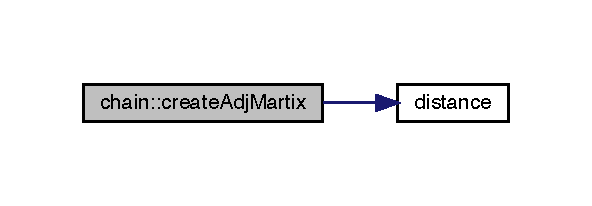
\includegraphics[width=284pt]{namespacechain_a68d5d08ece7d82a6b4bb1968b783a8f3_cgraph}
\end{center}
\end{figure}
Here is the caller graph for this function\+:\nopagebreak
\begin{figure}[H]
\begin{center}
\leavevmode
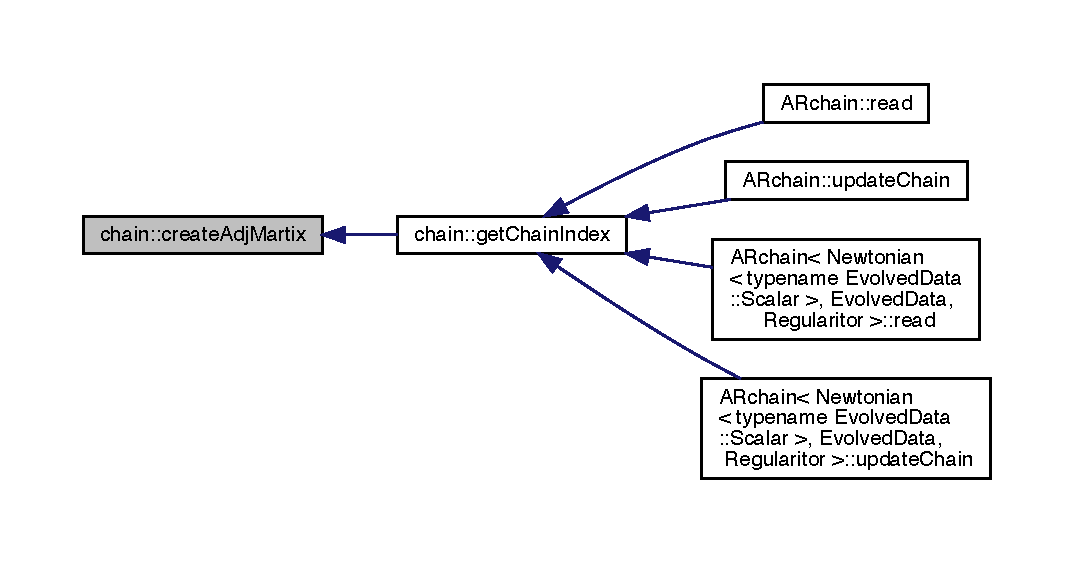
\includegraphics[width=350pt]{namespacechain_a68d5d08ece7d82a6b4bb1968b783a8f3_icgraph}
\end{center}
\end{figure}
\mbox{\Hypertarget{namespacechain_ae008a8273beabf1473c347994197ef53}\label{namespacechain_ae008a8273beabf1473c347994197ef53}} 
\index{chain@{chain}!create\+Chain\+Index@{create\+Chain\+Index}}
\index{create\+Chain\+Index@{create\+Chain\+Index}!chain@{chain}}
\paragraph{\texorpdfstring{create\+Chain\+Index()}{createChainIndex()}}
{\footnotesize\ttfamily template$<$typename Scalar , size\+\_\+t N$>$ \\
void chain\+::create\+Chain\+Index (\begin{DoxyParamCaption}\item[{\mbox{\hyperlink{namespacechain_a3a021b84403e03113e1dcd61ba304963}{Node\+Array}}$<$ Scalar, N $\ast$(N -\/ 1)/2 $>$ \&}]{Adj\+Matrix,  }\item[{\mbox{\hyperlink{namespacechain_aa40d2da395c0ac2bc5f37832442ac403}{Index\+Array}}$<$ N $>$ \&}]{chain\+Index }\end{DoxyParamCaption})}



Create mapping index from adjoint matrix. 

Create mapping index from sorted elements of adjoint matrix and connect them to a chain consequently. 
\begin{DoxyParams}{Parameters}
{\em Adj\+Matrix} & The adjoint matrix. \\
\hline
{\em chain\+Index} & The maping index needs to be calculated as a return value. \\
\hline
\end{DoxyParams}
Here is the caller graph for this function\+:\nopagebreak
\begin{figure}[H]
\begin{center}
\leavevmode
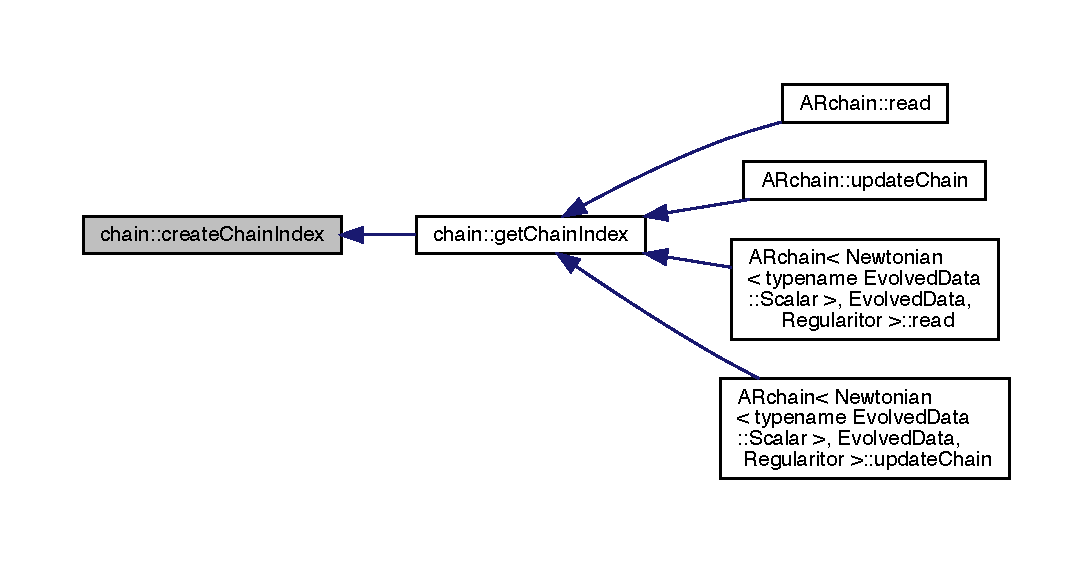
\includegraphics[width=350pt]{namespacechain_ae008a8273beabf1473c347994197ef53_icgraph}
\end{center}
\end{figure}
\mbox{\Hypertarget{namespacechain_a3e7b0a001442f121ce1408e7c9d12016}\label{namespacechain_a3e7b0a001442f121ce1408e7c9d12016}} 
\index{chain@{chain}!get\+Chain\+Index@{get\+Chain\+Index}}
\index{get\+Chain\+Index@{get\+Chain\+Index}!chain@{chain}}
\paragraph{\texorpdfstring{get\+Chain\+Index()}{getChainIndex()}}
{\footnotesize\ttfamily template$<$typename Scalar , size\+\_\+t N$>$ \\
void chain\+::get\+Chain\+Index (\begin{DoxyParamCaption}\item[{const \mbox{\hyperlink{namespacechain_aa715d2f046187ea9f0c3ea55605d6214}{Vector\+Array}}$<$ Scalar, N $>$ \&}]{pos,  }\item[{\mbox{\hyperlink{namespacechain_aa40d2da395c0ac2bc5f37832442ac403}{Index\+Array}}$<$ N $>$ \&}]{chain\+Index }\end{DoxyParamCaption})}



Calculate the mapping index from Cartesian coordinate to chain coordinate. 

Find the mapping index from Cartesian coordinate to chain coordinate. The chain is formed by connecting the nearest particle pairs consequently. 
\begin{DoxyParams}{Parameters}
{\em pos} & The array of particle position, used to calculate the distance of particle pairs. \\
\hline
{\em chain\+Index} & The maping index needs to be calculated as a return value. \\
\hline
\end{DoxyParams}
Here is the call graph for this function\+:\nopagebreak
\begin{figure}[H]
\begin{center}
\leavevmode
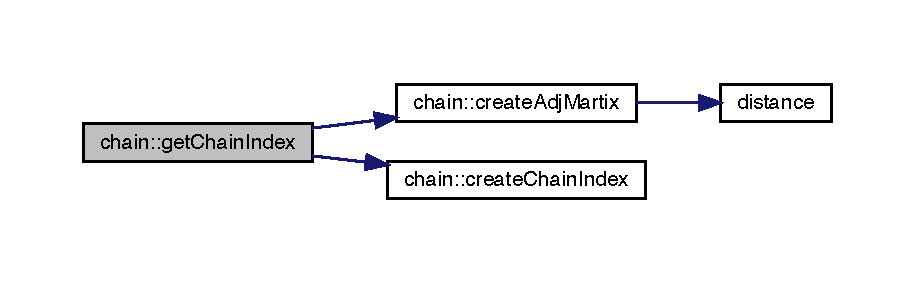
\includegraphics[width=350pt]{namespacechain_a3e7b0a001442f121ce1408e7c9d12016_cgraph}
\end{center}
\end{figure}
Here is the caller graph for this function\+:\nopagebreak
\begin{figure}[H]
\begin{center}
\leavevmode
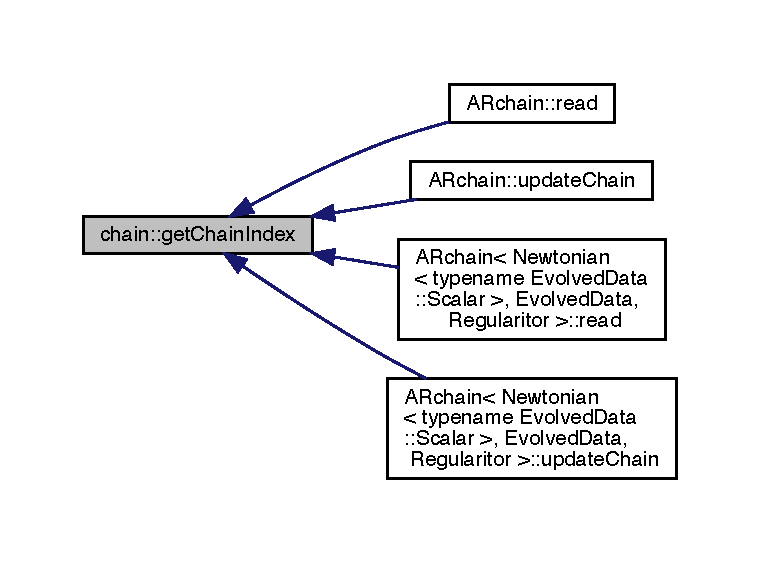
\includegraphics[width=350pt]{namespacechain_a3e7b0a001442f121ce1408e7c9d12016_icgraph}
\end{center}
\end{figure}
\mbox{\Hypertarget{namespacechain_a874f28a6248b56c6b2b3ca45c1bbea09}\label{namespacechain_a874f28a6248b56c6b2b3ca45c1bbea09}} 
\index{chain@{chain}!Is\+Diff@{Is\+Diff}}
\index{Is\+Diff@{Is\+Diff}!chain@{chain}}
\paragraph{\texorpdfstring{Is\+Diff()}{IsDiff()}}
{\footnotesize\ttfamily template$<$size\+\_\+t N$>$ \\
bool chain\+::\+Is\+Diff (\begin{DoxyParamCaption}\item[{const \mbox{\hyperlink{namespacechain_aa40d2da395c0ac2bc5f37832442ac403}{Index\+Array}}$<$ N $>$ \&}]{Index1,  }\item[{const \mbox{\hyperlink{namespacechain_aa40d2da395c0ac2bc5f37832442ac403}{Index\+Array}}$<$ N $>$ \&}]{Index2 }\end{DoxyParamCaption})}



Check if two mapping indexes are the same. 

Checking the identity of two chain index mappings. 
\begin{DoxyParams}{Parameters}
{\em Index1} & The first index array. \\
\hline
{\em Index2} & The second index array. \\
\hline
\end{DoxyParams}
\begin{DoxyReturn}{Returns}
boolean 
\end{DoxyReturn}
\begin{DoxyNote}{Note}
\mbox{[}2,4,5,3,1\mbox{]} is identical to \mbox{[}1,3,5,4,2\mbox{]} 
\end{DoxyNote}
Here is the caller graph for this function\+:\nopagebreak
\begin{figure}[H]
\begin{center}
\leavevmode
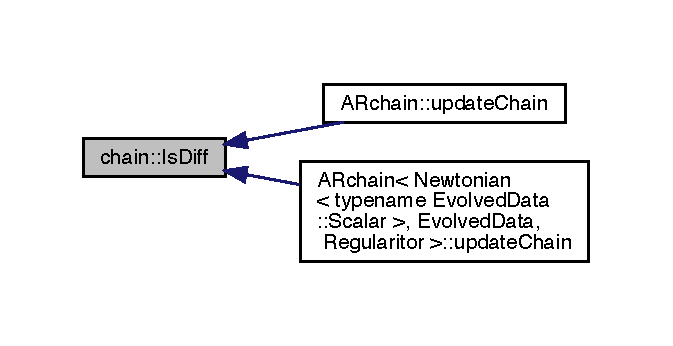
\includegraphics[width=323pt]{namespacechain_a874f28a6248b56c6b2b3ca45c1bbea09_icgraph}
\end{center}
\end{figure}
\mbox{\Hypertarget{namespacechain_ae85619534182ce257fc47857a9c133e4}\label{namespacechain_ae85619534182ce257fc47857a9c133e4}} 
\index{chain@{chain}!syn\+Cartesian@{syn\+Cartesian}}
\index{syn\+Cartesian@{syn\+Cartesian}!chain@{chain}}
\paragraph{\texorpdfstring{syn\+Cartesian()}{synCartesian()}}
{\footnotesize\ttfamily template$<$typename Scalar , size\+\_\+t N$>$ \\
void chain\+::syn\+Cartesian (\begin{DoxyParamCaption}\item[{\mbox{\hyperlink{namespacechain_aa715d2f046187ea9f0c3ea55605d6214}{Vector\+Array}}$<$ Scalar, N $>$ \&}]{chain\+Data,  }\item[{\mbox{\hyperlink{namespacechain_aa715d2f046187ea9f0c3ea55605d6214}{Vector\+Array}}$<$ Scalar, N $>$ \&}]{data,  }\item[{\mbox{\hyperlink{namespacechain_aa40d2da395c0ac2bc5f37832442ac403}{Index\+Array}}$<$ N $>$ \&}]{chain\+Index }\end{DoxyParamCaption})}



Calulate the Cartesian data from chain data and chain index mapping. 


\begin{DoxyParams}{Parameters}
{\em chain\+Data} & Data in chain coordinates. \\
\hline
{\em data} & Data need to be calculated in Cartesian coordinates. \\
\hline
{\em chain\+Index} & Chain index mapping. \\
\hline
\end{DoxyParams}
\begin{DoxyNote}{Note}
This function should be a inverse transformation of \mbox{\hyperlink{namespacechain_abdcb44461ef66afb82d42ff5a441ed5c}{syn\+Chain()}}. 
\end{DoxyNote}
Here is the caller graph for this function\+:\nopagebreak
\begin{figure}[H]
\begin{center}
\leavevmode
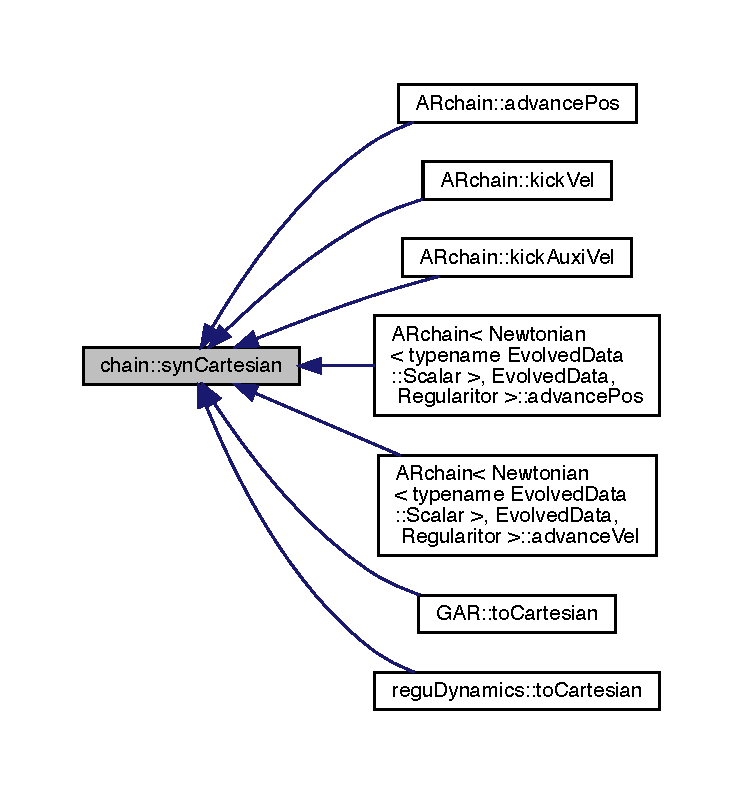
\includegraphics[width=350pt]{namespacechain_ae85619534182ce257fc47857a9c133e4_icgraph}
\end{center}
\end{figure}
\mbox{\Hypertarget{namespacechain_abdcb44461ef66afb82d42ff5a441ed5c}\label{namespacechain_abdcb44461ef66afb82d42ff5a441ed5c}} 
\index{chain@{chain}!syn\+Chain@{syn\+Chain}}
\index{syn\+Chain@{syn\+Chain}!chain@{chain}}
\paragraph{\texorpdfstring{syn\+Chain()}{synChain()}}
{\footnotesize\ttfamily template$<$typename Scalar , size\+\_\+t N$>$ \\
void chain\+::syn\+Chain (\begin{DoxyParamCaption}\item[{\mbox{\hyperlink{namespacechain_aa715d2f046187ea9f0c3ea55605d6214}{Vector\+Array}}$<$ Scalar, N $>$ \&}]{data,  }\item[{\mbox{\hyperlink{namespacechain_aa715d2f046187ea9f0c3ea55605d6214}{Vector\+Array}}$<$ Scalar, N $>$ \&}]{chain\+Data,  }\item[{\mbox{\hyperlink{namespacechain_aa40d2da395c0ac2bc5f37832442ac403}{Index\+Array}}$<$ N $>$ \&}]{chain\+Index }\end{DoxyParamCaption})}



Calulate the chain data from Cartesian data and chain index mapping. 


\begin{DoxyParams}{Parameters}
{\em data} & Data in Cartesian coordinates. \\
\hline
{\em chain\+Data} & Data need to be calculated in chain coordinates. \\
\hline
{\em chain\+Index} & Chain index mapping. \\
\hline
\end{DoxyParams}
\begin{DoxyNote}{Note}
This function should be a inverse transformation of \mbox{\hyperlink{namespacechain_ae85619534182ce257fc47857a9c133e4}{syn\+Cartesian()}}. 
\end{DoxyNote}
Here is the caller graph for this function\+:\nopagebreak
\begin{figure}[H]
\begin{center}
\leavevmode
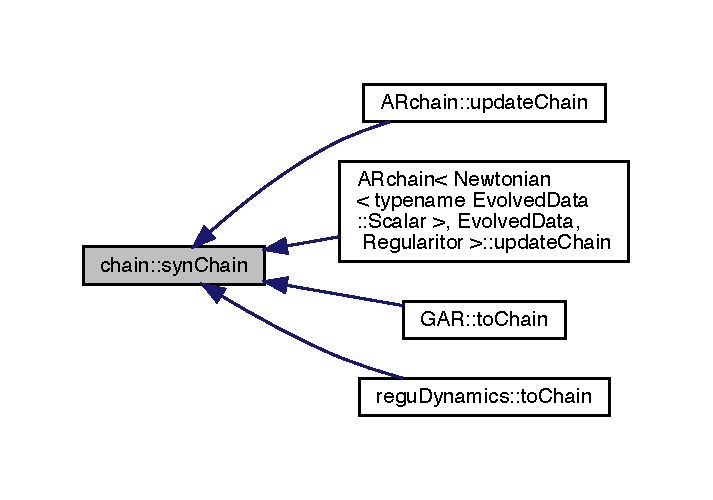
\includegraphics[width=342pt]{namespacechain_abdcb44461ef66afb82d42ff5a441ed5c_icgraph}
\end{center}
\end{figure}
\mbox{\Hypertarget{namespacechain_a36c1d242033be6243c1cff525f818724}\label{namespacechain_a36c1d242033be6243c1cff525f818724}} 
\index{chain@{chain}!update\+Chain@{update\+Chain}}
\index{update\+Chain@{update\+Chain}!chain@{chain}}
\paragraph{\texorpdfstring{update\+Chain()}{updateChain()}}
{\footnotesize\ttfamily template$<$typename Scalar , size\+\_\+t N$>$ \\
void chain\+::update\+Chain (\begin{DoxyParamCaption}\item[{\mbox{\hyperlink{namespacechain_aa715d2f046187ea9f0c3ea55605d6214}{Vector\+Array}}$<$ Scalar, N $>$ \&}]{pos,  }\item[{\mbox{\hyperlink{namespacechain_aa40d2da395c0ac2bc5f37832442ac403}{Index\+Array}}$<$ N $>$ \&}]{chain\+Index,  }\item[{\mbox{\hyperlink{namespacechain_aa40d2da395c0ac2bc5f37832442ac403}{Index\+Array}}$<$ N $>$ \&}]{new\+Index }\end{DoxyParamCaption})}



Update the position chain. 

Update the position chain. Due to the evolution, the chain index mapping could change with time, this function is used to update the position chain with old chain data. 
\begin{DoxyParams}{Parameters}
{\em pos} & The old chain position array needs update. \\
\hline
{\em chain\+Index} & The old chain index mapping. \\
\hline
{\em new\+Index} & The new chain index mapping. \\
\hline
\end{DoxyParams}
Here is the caller graph for this function\+:\nopagebreak
\begin{figure}[H]
\begin{center}
\leavevmode
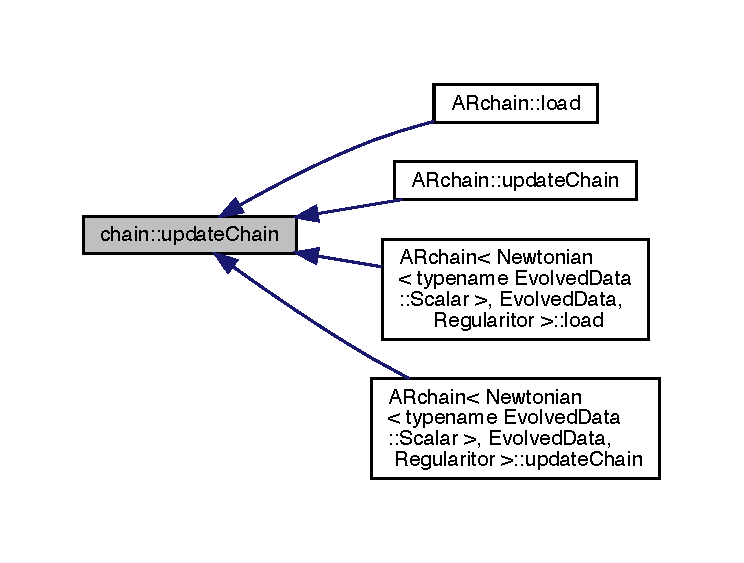
\includegraphics[width=350pt]{namespacechain_a36c1d242033be6243c1cff525f818724_icgraph}
\end{center}
\end{figure}

\hypertarget{namespace_n_o_t_i_c_e}{}\section{N\+O\+T\+I\+CE Namespace Reference}
\label{namespace_n_o_t_i_c_e}\index{N\+O\+T\+I\+CE@{N\+O\+T\+I\+CE}}
\subsection*{Functions}
\begin{DoxyCompactItemize}
\item 
void \mbox{\hyperlink{namespace_n_o_t_i_c_e_a7f45e7bbaeb797160d77c7c5dbbb37a6}{Telegram}} (const char $\ast$host, const char $\ast$msg)
\item 
void \mbox{\hyperlink{namespace_n_o_t_i_c_e_a0ddfb0ca7dfa968616d34f4752368bba}{Title}} (const char $\ast$T)
\item 
void \mbox{\hyperlink{namespace_n_o_t_i_c_e_a483b62c015a4211e2716f730ad2c0a44}{Sub\+Title}} (const char $\ast$T)
\item 
void \mbox{\hyperlink{namespace_n_o_t_i_c_e_a46fcf4944d7c1d3cc4d821297b0e4bf8}{Erase\+Line}} ()
\item 
void \mbox{\hyperlink{namespace_n_o_t_i_c_e_a9536e3b7bb1f9b6af83b1a5cdf3a56d3}{Line}} ()
\item 
void \mbox{\hyperlink{namespace_n_o_t_i_c_e_a782778073f9df89a3d20a7faa16494aa}{Sub\+Line}} ()
\item 
void \mbox{\hyperlink{namespace_n_o_t_i_c_e_ab85b7138c5f1deaeeedad94b7bad2477}{Run\+Info}} (double time\+Limit, double outputsize\+\_\+terval, double tolerance)
\end{DoxyCompactItemize}
\subsection*{Variables}
\begin{DoxyCompactItemize}
\item 
constexpr size\+\_\+t \mbox{\hyperlink{namespace_n_o_t_i_c_e_a31f6fb221f22faf96b9cfb05315d1d3e}{W\+I\+D\+TH}} = 80
\item 
bool \mbox{\hyperlink{namespace_n_o_t_i_c_e_a4de9d52506c4de1641e95f4f53669e3f}{Message}} = true
\end{DoxyCompactItemize}


\subsection{Function Documentation}
\mbox{\Hypertarget{namespace_n_o_t_i_c_e_a46fcf4944d7c1d3cc4d821297b0e4bf8}\label{namespace_n_o_t_i_c_e_a46fcf4944d7c1d3cc4d821297b0e4bf8}} 
\index{N\+O\+T\+I\+CE@{N\+O\+T\+I\+CE}!Erase\+Line@{Erase\+Line}}
\index{Erase\+Line@{Erase\+Line}!N\+O\+T\+I\+CE@{N\+O\+T\+I\+CE}}
\subsubsection{\texorpdfstring{Erase\+Line()}{EraseLine()}}
{\footnotesize\ttfamily void N\+O\+T\+I\+C\+E\+::\+Erase\+Line (\begin{DoxyParamCaption}{ }\end{DoxyParamCaption})\hspace{0.3cm}{\ttfamily [inline]}}

\mbox{\Hypertarget{namespace_n_o_t_i_c_e_a9536e3b7bb1f9b6af83b1a5cdf3a56d3}\label{namespace_n_o_t_i_c_e_a9536e3b7bb1f9b6af83b1a5cdf3a56d3}} 
\index{N\+O\+T\+I\+CE@{N\+O\+T\+I\+CE}!Line@{Line}}
\index{Line@{Line}!N\+O\+T\+I\+CE@{N\+O\+T\+I\+CE}}
\subsubsection{\texorpdfstring{Line()}{Line()}}
{\footnotesize\ttfamily void N\+O\+T\+I\+C\+E\+::\+Line (\begin{DoxyParamCaption}{ }\end{DoxyParamCaption})\hspace{0.3cm}{\ttfamily [inline]}}

\mbox{\Hypertarget{namespace_n_o_t_i_c_e_ab85b7138c5f1deaeeedad94b7bad2477}\label{namespace_n_o_t_i_c_e_ab85b7138c5f1deaeeedad94b7bad2477}} 
\index{N\+O\+T\+I\+CE@{N\+O\+T\+I\+CE}!Run\+Info@{Run\+Info}}
\index{Run\+Info@{Run\+Info}!N\+O\+T\+I\+CE@{N\+O\+T\+I\+CE}}
\subsubsection{\texorpdfstring{Run\+Info()}{RunInfo()}}
{\footnotesize\ttfamily void N\+O\+T\+I\+C\+E\+::\+Run\+Info (\begin{DoxyParamCaption}\item[{double}]{time\+Limit,  }\item[{double}]{outputsize\+\_\+terval,  }\item[{double}]{tolerance }\end{DoxyParamCaption})\hspace{0.3cm}{\ttfamily [inline]}}

\mbox{\Hypertarget{namespace_n_o_t_i_c_e_a782778073f9df89a3d20a7faa16494aa}\label{namespace_n_o_t_i_c_e_a782778073f9df89a3d20a7faa16494aa}} 
\index{N\+O\+T\+I\+CE@{N\+O\+T\+I\+CE}!Sub\+Line@{Sub\+Line}}
\index{Sub\+Line@{Sub\+Line}!N\+O\+T\+I\+CE@{N\+O\+T\+I\+CE}}
\subsubsection{\texorpdfstring{Sub\+Line()}{SubLine()}}
{\footnotesize\ttfamily void N\+O\+T\+I\+C\+E\+::\+Sub\+Line (\begin{DoxyParamCaption}{ }\end{DoxyParamCaption})\hspace{0.3cm}{\ttfamily [inline]}}

\mbox{\Hypertarget{namespace_n_o_t_i_c_e_a483b62c015a4211e2716f730ad2c0a44}\label{namespace_n_o_t_i_c_e_a483b62c015a4211e2716f730ad2c0a44}} 
\index{N\+O\+T\+I\+CE@{N\+O\+T\+I\+CE}!Sub\+Title@{Sub\+Title}}
\index{Sub\+Title@{Sub\+Title}!N\+O\+T\+I\+CE@{N\+O\+T\+I\+CE}}
\subsubsection{\texorpdfstring{Sub\+Title()}{SubTitle()}}
{\footnotesize\ttfamily void N\+O\+T\+I\+C\+E\+::\+Sub\+Title (\begin{DoxyParamCaption}\item[{const char $\ast$}]{T }\end{DoxyParamCaption})\hspace{0.3cm}{\ttfamily [inline]}}

\mbox{\Hypertarget{namespace_n_o_t_i_c_e_a7f45e7bbaeb797160d77c7c5dbbb37a6}\label{namespace_n_o_t_i_c_e_a7f45e7bbaeb797160d77c7c5dbbb37a6}} 
\index{N\+O\+T\+I\+CE@{N\+O\+T\+I\+CE}!Telegram@{Telegram}}
\index{Telegram@{Telegram}!N\+O\+T\+I\+CE@{N\+O\+T\+I\+CE}}
\subsubsection{\texorpdfstring{Telegram()}{Telegram()}}
{\footnotesize\ttfamily void N\+O\+T\+I\+C\+E\+::\+Telegram (\begin{DoxyParamCaption}\item[{const char $\ast$}]{host,  }\item[{const char $\ast$}]{msg }\end{DoxyParamCaption})\hspace{0.3cm}{\ttfamily [inline]}}

\mbox{\Hypertarget{namespace_n_o_t_i_c_e_a0ddfb0ca7dfa968616d34f4752368bba}\label{namespace_n_o_t_i_c_e_a0ddfb0ca7dfa968616d34f4752368bba}} 
\index{N\+O\+T\+I\+CE@{N\+O\+T\+I\+CE}!Title@{Title}}
\index{Title@{Title}!N\+O\+T\+I\+CE@{N\+O\+T\+I\+CE}}
\subsubsection{\texorpdfstring{Title()}{Title()}}
{\footnotesize\ttfamily void N\+O\+T\+I\+C\+E\+::\+Title (\begin{DoxyParamCaption}\item[{const char $\ast$}]{T }\end{DoxyParamCaption})\hspace{0.3cm}{\ttfamily [inline]}}



\subsection{Variable Documentation}
\mbox{\Hypertarget{namespace_n_o_t_i_c_e_a4de9d52506c4de1641e95f4f53669e3f}\label{namespace_n_o_t_i_c_e_a4de9d52506c4de1641e95f4f53669e3f}} 
\index{N\+O\+T\+I\+CE@{N\+O\+T\+I\+CE}!Message@{Message}}
\index{Message@{Message}!N\+O\+T\+I\+CE@{N\+O\+T\+I\+CE}}
\subsubsection{\texorpdfstring{Message}{Message}}
{\footnotesize\ttfamily bool N\+O\+T\+I\+C\+E\+::\+Message = true}

\mbox{\Hypertarget{namespace_n_o_t_i_c_e_a31f6fb221f22faf96b9cfb05315d1d3e}\label{namespace_n_o_t_i_c_e_a31f6fb221f22faf96b9cfb05315d1d3e}} 
\index{N\+O\+T\+I\+CE@{N\+O\+T\+I\+CE}!W\+I\+D\+TH@{W\+I\+D\+TH}}
\index{W\+I\+D\+TH@{W\+I\+D\+TH}!N\+O\+T\+I\+CE@{N\+O\+T\+I\+CE}}
\subsubsection{\texorpdfstring{W\+I\+D\+TH}{WIDTH}}
{\footnotesize\ttfamily constexpr size\+\_\+t N\+O\+T\+I\+C\+E\+::\+W\+I\+D\+TH = 80}


\chapter{Class Documentation}
\hypertarget{class_a_rchain}{}\section{A\+Rchain$<$ Interaction, Evolved\+Data, Regularitor $>$ Class Template Reference}
\label{class_a_rchain}\index{A\+Rchain$<$ Interaction, Evolved\+Data, Regularitor $>$@{A\+Rchain$<$ Interaction, Evolved\+Data, Regularitor $>$}}


{\ttfamily \#include $<$A\+Rchain.\+h$>$}



Inheritance diagram for A\+Rchain$<$ Interaction, Evolved\+Data, Regularitor $>$\+:\nopagebreak
\begin{figure}[H]
\begin{center}
\leavevmode
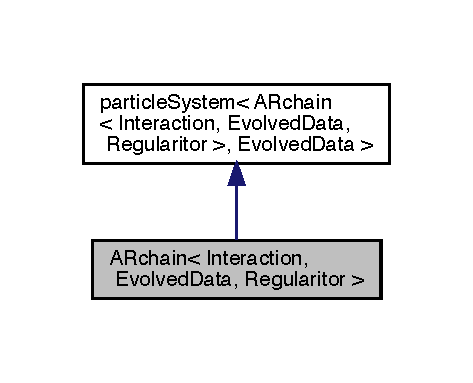
\includegraphics[width=227pt]{class_a_rchain__inherit__graph}
\end{center}
\end{figure}


Collaboration diagram for A\+Rchain$<$ Interaction, Evolved\+Data, Regularitor $>$\+:
\nopagebreak
\begin{figure}[H]
\begin{center}
\leavevmode
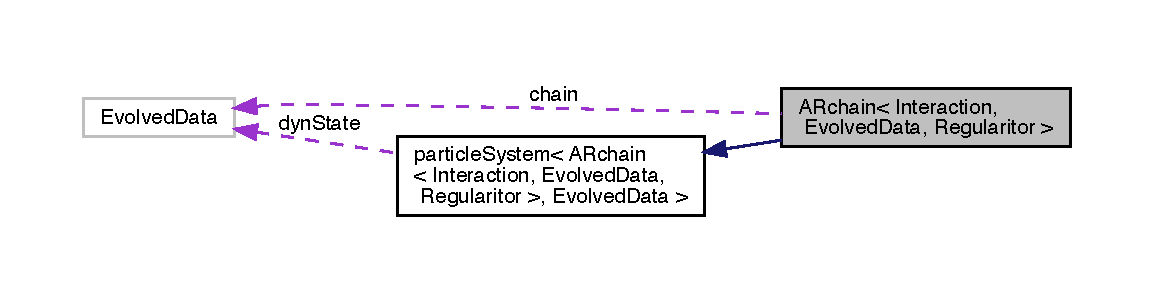
\includegraphics[width=350pt]{class_a_rchain__coll__graph}
\end{center}
\end{figure}
\subsection*{Public Types}
\begin{DoxyCompactItemize}
\item 
typedef Evolved\+Data\+::\+Scalar \mbox{\hyperlink{class_a_rchain_a707e42a79e4744424a34c9007e84ee07}{Scalar}}
\item 
typedef Evolved\+Data\+::\+Vector \mbox{\hyperlink{class_a_rchain_ab9b518a463f750eb54e002842b66e8dd}{Vector}}
\item 
typedef Evolved\+Data\+::\+Vector\+Array \mbox{\hyperlink{class_a_rchain_a019fbadb9f4e5892736d9127537338bb}{Vector\+Array}}
\item 
typedef Evolved\+Data\+::\+Scalar\+Array \mbox{\hyperlink{class_a_rchain_a206c7f2ff7ce15041a20d327d28b7be3}{Scalar\+Array}}
\item 
typedef std\+::array$<$ size\+\_\+t, Evolved\+Data\+::size()$>$ \mbox{\hyperlink{class_a_rchain_aae40d4b5881eecfc960814f9e368215d}{Index\+Array}}
\item 
typedef std\+::array$<$ \mbox{\hyperlink{class_a_rchain_a707e42a79e4744424a34c9007e84ee07}{Scalar}}, Evolved\+Data\+::volume()$>$ \mbox{\hyperlink{class_a_rchain_a829aca51411c08ffd518294770a374d5}{Plain\+Array}}
\end{DoxyCompactItemize}
\subsection*{Public Member Functions}
\begin{DoxyCompactItemize}
\item 
void \mbox{\hyperlink{class_a_rchain_a8d3ac75a6b4231e0859492257553316e}{advance\+Pos}} (\mbox{\hyperlink{class_a_rchain_a707e42a79e4744424a34c9007e84ee07}{Scalar}} time\+Step\+Size)
\item 
void \mbox{\hyperlink{class_a_rchain_a6a76ab7a095adfbf4a69226a31d866d4}{advance\+Vel}} (\mbox{\hyperlink{class_a_rchain_a707e42a79e4744424a34c9007e84ee07}{Scalar}} time\+Step\+Size)
\item 
const \mbox{\hyperlink{class_a_rchain}{A\+Rchain}} \& \mbox{\hyperlink{class_a_rchain_a7bcc783f99cad1e9113d2b505544aba1}{operator=}} (const \mbox{\hyperlink{class_a_rchain}{A\+Rchain}} \&other)
\item 
std\+::istream \& \mbox{\hyperlink{class_a_rchain_a86bd89bacf59c9c3bb0594499db82e04}{read}} (std\+::istream \&)
\item 
void \mbox{\hyperlink{class_a_rchain_a7edf1240a094d55df222c816659dced0}{load}} (\mbox{\hyperlink{class_a_rchain_a829aca51411c08ffd518294770a374d5}{Plain\+Array}} \&data)
\item 
\mbox{\hyperlink{class_a_rchain_a707e42a79e4744424a34c9007e84ee07}{Scalar}} \mbox{\hyperlink{class_a_rchain_a979a40abd086aeb411dc8e82a3bb1cdf}{time\+Scale}} (\mbox{\hyperlink{class_a_rchain_a707e42a79e4744424a34c9007e84ee07}{Scalar}} scale)
\item 
\mbox{\hyperlink{class_a_rchain_a829aca51411c08ffd518294770a374d5}{Plain\+Array}} \& \mbox{\hyperlink{class_a_rchain_aeb4d9b0a28ae3b4e4286edf838e5a905}{array}} ()
\end{DoxyCompactItemize}
\subsection*{Static Public Member Functions}
\begin{DoxyCompactItemize}
\item 
static constexpr size\+\_\+t \mbox{\hyperlink{class_a_rchain_ac612af46ce057d56dc47a6d28738a4cf}{size}} ()
\end{DoxyCompactItemize}
\subsection*{Private Member Functions}
\begin{DoxyCompactItemize}
\item 
void \mbox{\hyperlink{class_a_rchain_ac54722bde3c9a15e04dd004ebcf0db5e}{advance\+Omega}} (\mbox{\hyperlink{class_a_rchain_a707e42a79e4744424a34c9007e84ee07}{Scalar}} step\+Size)
\item 
void \mbox{\hyperlink{class_a_rchain_a1b2ae6231caeba3df20e4ab41f63a4b8}{advanceB}} (\mbox{\hyperlink{class_a_rchain_a707e42a79e4744424a34c9007e84ee07}{Scalar}} step\+Size)
\item 
void \mbox{\hyperlink{class_a_rchain_a0b073cd82321047d7fafda59cef998ef}{kick\+Vel}} (\mbox{\hyperlink{class_a_rchain_a707e42a79e4744424a34c9007e84ee07}{Scalar}} step\+Size)
\item 
void \mbox{\hyperlink{class_a_rchain_a53838a7890cee54c69786bda87dd6cd9}{kick\+Auxi\+Vel}} (\mbox{\hyperlink{class_a_rchain_a707e42a79e4744424a34c9007e84ee07}{Scalar}} step\+Size)
\item 
void \mbox{\hyperlink{class_a_rchain_a92865bff07dc16e3065a8f695120a5f5}{update\+Acc\+With}} (\mbox{\hyperlink{class_a_rchain_a019fbadb9f4e5892736d9127537338bb}{Vector\+Array}} \&\mbox{\hyperlink{classparticle_system_a545da170c4d59f18c6ddb18817cb5f3e}{vel}}, \mbox{\hyperlink{class_a_rchain_a019fbadb9f4e5892736d9127537338bb}{Vector\+Array}} \&chain\+Vel)
\item 
void \mbox{\hyperlink{class_a_rchain_a08ddf32fb537ac1556b2e4560abf3b5d}{update\+Vel\+Indep\+Acc}} ()
\item 
void \mbox{\hyperlink{class_a_rchain_ad576df000b6d9f3948eae2793c6b3c54}{update\+Chain}} ()
\end{DoxyCompactItemize}
\subsection*{Private Attributes}
\begin{DoxyCompactItemize}
\item 
Evolved\+Data \mbox{\hyperlink{class_a_rchain_af7780024bfc1beca5f5622086b909db2}{chain}}
\item 
\mbox{\hyperlink{class_a_rchain_aae40d4b5881eecfc960814f9e368215d}{Index\+Array}} \mbox{\hyperlink{class_a_rchain_a0691e6612b661e329f1fc72d4cb7c895}{chain\+Index}}
\item 
\mbox{\hyperlink{class_a_rchain_a019fbadb9f4e5892736d9127537338bb}{Vector\+Array}} \mbox{\hyperlink{class_a_rchain_a9359b4fb9f08ad849b0f1dfbdf661016}{vel\+Indep\+Acc}}
\item 
\mbox{\hyperlink{class_a_rchain_a019fbadb9f4e5892736d9127537338bb}{Vector\+Array}} \mbox{\hyperlink{class_a_rchain_a80d060a3341913f94c4bbbf2e2321b1d}{chain\+Vel\+Indep\+Acc}}
\item 
\mbox{\hyperlink{class_a_rchain_a019fbadb9f4e5892736d9127537338bb}{Vector\+Array}} \mbox{\hyperlink{class_a_rchain_a3c3a74f839bbfe5cbe1d8eb239dd8cc1}{vel\+Dep\+Acc}}
\item 
\mbox{\hyperlink{class_a_rchain_a019fbadb9f4e5892736d9127537338bb}{Vector\+Array}} \mbox{\hyperlink{class_a_rchain_a64087e0cb9cdb6b118b4a6e416d9f012}{chain\+Vel\+Dep\+Acc}}
\item 
Interaction \mbox{\hyperlink{class_a_rchain_a5ad11cefbdb69a58225b799b36dd9eee}{vel\+Dep\+Force}}
\item 
Regularitor \mbox{\hyperlink{class_a_rchain_a4dd20aa56d6a6403260ad3ced2987eb0}{regular}}
\end{DoxyCompactItemize}
\subsection*{Additional Inherited Members}


\subsection{Member Typedef Documentation}
\mbox{\Hypertarget{class_a_rchain_aae40d4b5881eecfc960814f9e368215d}\label{class_a_rchain_aae40d4b5881eecfc960814f9e368215d}} 
\index{A\+Rchain@{A\+Rchain}!Index\+Array@{Index\+Array}}
\index{Index\+Array@{Index\+Array}!A\+Rchain@{A\+Rchain}}
\subsubsection{\texorpdfstring{Index\+Array}{IndexArray}}
{\footnotesize\ttfamily template$<$typename Interaction, typename Evolved\+Data, typename Regularitor$>$ \\
typedef std\+::array$<$size\+\_\+t, Evolved\+Data\+::size()$>$ \mbox{\hyperlink{class_a_rchain}{A\+Rchain}}$<$ Interaction, Evolved\+Data, Regularitor $>$\+::\mbox{\hyperlink{class_a_rchain_aae40d4b5881eecfc960814f9e368215d}{Index\+Array}}}

\mbox{\Hypertarget{class_a_rchain_a829aca51411c08ffd518294770a374d5}\label{class_a_rchain_a829aca51411c08ffd518294770a374d5}} 
\index{A\+Rchain@{A\+Rchain}!Plain\+Array@{Plain\+Array}}
\index{Plain\+Array@{Plain\+Array}!A\+Rchain@{A\+Rchain}}
\subsubsection{\texorpdfstring{Plain\+Array}{PlainArray}}
{\footnotesize\ttfamily template$<$typename Interaction, typename Evolved\+Data, typename Regularitor$>$ \\
typedef std\+::array$<$\mbox{\hyperlink{class_a_rchain_a707e42a79e4744424a34c9007e84ee07}{Scalar}}, Evolved\+Data\+::volume()$>$ \mbox{\hyperlink{class_a_rchain}{A\+Rchain}}$<$ Interaction, Evolved\+Data, Regularitor $>$\+::\mbox{\hyperlink{class_a_rchain_a829aca51411c08ffd518294770a374d5}{Plain\+Array}}}

\mbox{\Hypertarget{class_a_rchain_a707e42a79e4744424a34c9007e84ee07}\label{class_a_rchain_a707e42a79e4744424a34c9007e84ee07}} 
\index{A\+Rchain@{A\+Rchain}!Scalar@{Scalar}}
\index{Scalar@{Scalar}!A\+Rchain@{A\+Rchain}}
\subsubsection{\texorpdfstring{Scalar}{Scalar}}
{\footnotesize\ttfamily template$<$typename Interaction, typename Evolved\+Data, typename Regularitor$>$ \\
typedef Evolved\+Data\+::\+Scalar \mbox{\hyperlink{class_a_rchain}{A\+Rchain}}$<$ Interaction, Evolved\+Data, Regularitor $>$\+::\mbox{\hyperlink{class_a_rchain_a707e42a79e4744424a34c9007e84ee07}{Scalar}}}

\mbox{\Hypertarget{class_a_rchain_a206c7f2ff7ce15041a20d327d28b7be3}\label{class_a_rchain_a206c7f2ff7ce15041a20d327d28b7be3}} 
\index{A\+Rchain@{A\+Rchain}!Scalar\+Array@{Scalar\+Array}}
\index{Scalar\+Array@{Scalar\+Array}!A\+Rchain@{A\+Rchain}}
\subsubsection{\texorpdfstring{Scalar\+Array}{ScalarArray}}
{\footnotesize\ttfamily template$<$typename Interaction, typename Evolved\+Data, typename Regularitor$>$ \\
typedef Evolved\+Data\+::\+Scalar\+Array \mbox{\hyperlink{class_a_rchain}{A\+Rchain}}$<$ Interaction, Evolved\+Data, Regularitor $>$\+::\mbox{\hyperlink{class_a_rchain_a206c7f2ff7ce15041a20d327d28b7be3}{Scalar\+Array}}}

\mbox{\Hypertarget{class_a_rchain_ab9b518a463f750eb54e002842b66e8dd}\label{class_a_rchain_ab9b518a463f750eb54e002842b66e8dd}} 
\index{A\+Rchain@{A\+Rchain}!Vector@{Vector}}
\index{Vector@{Vector}!A\+Rchain@{A\+Rchain}}
\subsubsection{\texorpdfstring{Vector}{Vector}}
{\footnotesize\ttfamily template$<$typename Interaction, typename Evolved\+Data, typename Regularitor$>$ \\
typedef Evolved\+Data\+::\+Vector \mbox{\hyperlink{class_a_rchain}{A\+Rchain}}$<$ Interaction, Evolved\+Data, Regularitor $>$\+::\mbox{\hyperlink{class_a_rchain_ab9b518a463f750eb54e002842b66e8dd}{Vector}}}

\mbox{\Hypertarget{class_a_rchain_a019fbadb9f4e5892736d9127537338bb}\label{class_a_rchain_a019fbadb9f4e5892736d9127537338bb}} 
\index{A\+Rchain@{A\+Rchain}!Vector\+Array@{Vector\+Array}}
\index{Vector\+Array@{Vector\+Array}!A\+Rchain@{A\+Rchain}}
\subsubsection{\texorpdfstring{Vector\+Array}{VectorArray}}
{\footnotesize\ttfamily template$<$typename Interaction, typename Evolved\+Data, typename Regularitor$>$ \\
typedef Evolved\+Data\+::\+Vector\+Array \mbox{\hyperlink{class_a_rchain}{A\+Rchain}}$<$ Interaction, Evolved\+Data, Regularitor $>$\+::\mbox{\hyperlink{class_a_rchain_a019fbadb9f4e5892736d9127537338bb}{Vector\+Array}}}



\subsection{Member Function Documentation}
\mbox{\Hypertarget{class_a_rchain_a1b2ae6231caeba3df20e4ab41f63a4b8}\label{class_a_rchain_a1b2ae6231caeba3df20e4ab41f63a4b8}} 
\index{A\+Rchain@{A\+Rchain}!advanceB@{advanceB}}
\index{advanceB@{advanceB}!A\+Rchain@{A\+Rchain}}
\subsubsection{\texorpdfstring{advance\+B()}{advanceB()}}
{\footnotesize\ttfamily template$<$typename Interaction , typename Evolved\+Data , typename Regularitor $>$ \\
void \mbox{\hyperlink{class_a_rchain}{A\+Rchain}}$<$ Interaction, Evolved\+Data, Regularitor $>$\+::advanceB (\begin{DoxyParamCaption}\item[{\mbox{\hyperlink{class_a_rchain_a707e42a79e4744424a34c9007e84ee07}{Scalar}}}]{step\+Size }\end{DoxyParamCaption})\hspace{0.3cm}{\ttfamily [private]}}

Here is the call graph for this function\+:
\nopagebreak
\begin{figure}[H]
\begin{center}
\leavevmode
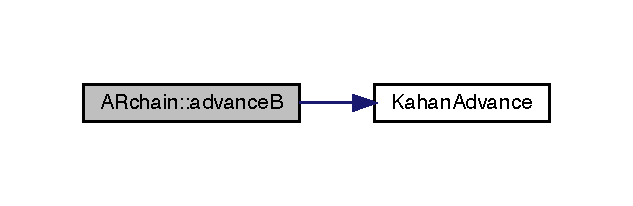
\includegraphics[width=304pt]{class_a_rchain_a1b2ae6231caeba3df20e4ab41f63a4b8_cgraph}
\end{center}
\end{figure}
\mbox{\Hypertarget{class_a_rchain_ac54722bde3c9a15e04dd004ebcf0db5e}\label{class_a_rchain_ac54722bde3c9a15e04dd004ebcf0db5e}} 
\index{A\+Rchain@{A\+Rchain}!advance\+Omega@{advance\+Omega}}
\index{advance\+Omega@{advance\+Omega}!A\+Rchain@{A\+Rchain}}
\subsubsection{\texorpdfstring{advance\+Omega()}{advanceOmega()}}
{\footnotesize\ttfamily template$<$typename Interaction , typename Evolved\+Data , typename Regularitor $>$ \\
void \mbox{\hyperlink{class_a_rchain}{A\+Rchain}}$<$ Interaction, Evolved\+Data, Regularitor $>$\+::advance\+Omega (\begin{DoxyParamCaption}\item[{\mbox{\hyperlink{class_a_rchain_a707e42a79e4744424a34c9007e84ee07}{Scalar}}}]{step\+Size }\end{DoxyParamCaption})\hspace{0.3cm}{\ttfamily [private]}}

Here is the call graph for this function\+:
\nopagebreak
\begin{figure}[H]
\begin{center}
\leavevmode
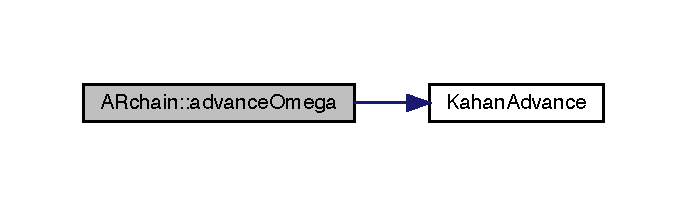
\includegraphics[width=330pt]{class_a_rchain_ac54722bde3c9a15e04dd004ebcf0db5e_cgraph}
\end{center}
\end{figure}
\mbox{\Hypertarget{class_a_rchain_a8d3ac75a6b4231e0859492257553316e}\label{class_a_rchain_a8d3ac75a6b4231e0859492257553316e}} 
\index{A\+Rchain@{A\+Rchain}!advance\+Pos@{advance\+Pos}}
\index{advance\+Pos@{advance\+Pos}!A\+Rchain@{A\+Rchain}}
\subsubsection{\texorpdfstring{advance\+Pos()}{advancePos()}}
{\footnotesize\ttfamily template$<$typename Interaction , typename Evolved\+Data , typename Regularitor $>$ \\
void \mbox{\hyperlink{class_a_rchain}{A\+Rchain}}$<$ Interaction, Evolved\+Data, Regularitor $>$\+::advance\+Pos (\begin{DoxyParamCaption}\item[{\mbox{\hyperlink{class_a_rchain_a707e42a79e4744424a34c9007e84ee07}{Scalar}}}]{time\+Step\+Size }\end{DoxyParamCaption})}

Here is the call graph for this function\+:
\nopagebreak
\begin{figure}[H]
\begin{center}
\leavevmode
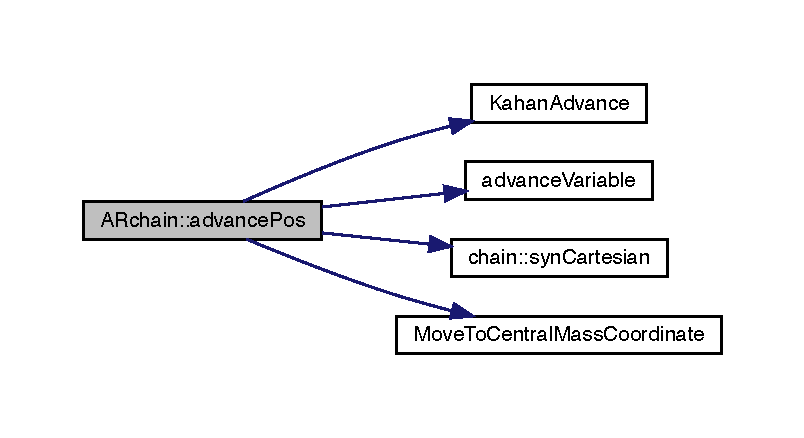
\includegraphics[width=350pt]{class_a_rchain_a8d3ac75a6b4231e0859492257553316e_cgraph}
\end{center}
\end{figure}
\mbox{\Hypertarget{class_a_rchain_a6a76ab7a095adfbf4a69226a31d866d4}\label{class_a_rchain_a6a76ab7a095adfbf4a69226a31d866d4}} 
\index{A\+Rchain@{A\+Rchain}!advance\+Vel@{advance\+Vel}}
\index{advance\+Vel@{advance\+Vel}!A\+Rchain@{A\+Rchain}}
\subsubsection{\texorpdfstring{advance\+Vel()}{advanceVel()}}
{\footnotesize\ttfamily template$<$typename Interaction , typename Evolved\+Data , typename Regularitor $>$ \\
void \mbox{\hyperlink{class_a_rchain}{A\+Rchain}}$<$ Interaction, Evolved\+Data, Regularitor $>$\+::advance\+Vel (\begin{DoxyParamCaption}\item[{\mbox{\hyperlink{class_a_rchain_a707e42a79e4744424a34c9007e84ee07}{Scalar}}}]{time\+Step\+Size }\end{DoxyParamCaption})}

\mbox{\Hypertarget{class_a_rchain_aeb4d9b0a28ae3b4e4286edf838e5a905}\label{class_a_rchain_aeb4d9b0a28ae3b4e4286edf838e5a905}} 
\index{A\+Rchain@{A\+Rchain}!array@{array}}
\index{array@{array}!A\+Rchain@{A\+Rchain}}
\subsubsection{\texorpdfstring{array()}{array()}}
{\footnotesize\ttfamily template$<$typename Interaction, typename Evolved\+Data, typename Regularitor$>$ \\
\mbox{\hyperlink{class_a_rchain_a829aca51411c08ffd518294770a374d5}{Plain\+Array}}\& \mbox{\hyperlink{class_a_rchain}{A\+Rchain}}$<$ Interaction, Evolved\+Data, Regularitor $>$\+::array (\begin{DoxyParamCaption}{ }\end{DoxyParamCaption})\hspace{0.3cm}{\ttfamily [inline]}}

\mbox{\Hypertarget{class_a_rchain_a53838a7890cee54c69786bda87dd6cd9}\label{class_a_rchain_a53838a7890cee54c69786bda87dd6cd9}} 
\index{A\+Rchain@{A\+Rchain}!kick\+Auxi\+Vel@{kick\+Auxi\+Vel}}
\index{kick\+Auxi\+Vel@{kick\+Auxi\+Vel}!A\+Rchain@{A\+Rchain}}
\subsubsection{\texorpdfstring{kick\+Auxi\+Vel()}{kickAuxiVel()}}
{\footnotesize\ttfamily template$<$typename Interaction , typename Evolved\+Data , typename Regularitor $>$ \\
void \mbox{\hyperlink{class_a_rchain}{A\+Rchain}}$<$ Interaction, Evolved\+Data, Regularitor $>$\+::kick\+Auxi\+Vel (\begin{DoxyParamCaption}\item[{\mbox{\hyperlink{class_a_rchain_a707e42a79e4744424a34c9007e84ee07}{Scalar}}}]{step\+Size }\end{DoxyParamCaption})\hspace{0.3cm}{\ttfamily [private]}}

Here is the call graph for this function\+:
\nopagebreak
\begin{figure}[H]
\begin{center}
\leavevmode
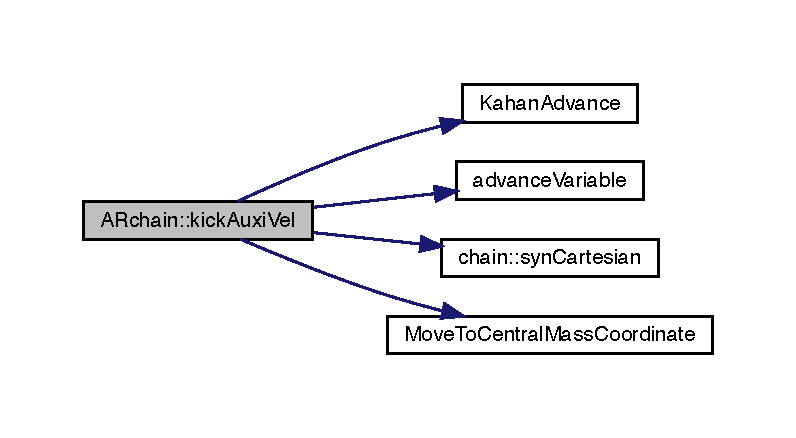
\includegraphics[width=350pt]{class_a_rchain_a53838a7890cee54c69786bda87dd6cd9_cgraph}
\end{center}
\end{figure}
\mbox{\Hypertarget{class_a_rchain_a0b073cd82321047d7fafda59cef998ef}\label{class_a_rchain_a0b073cd82321047d7fafda59cef998ef}} 
\index{A\+Rchain@{A\+Rchain}!kick\+Vel@{kick\+Vel}}
\index{kick\+Vel@{kick\+Vel}!A\+Rchain@{A\+Rchain}}
\subsubsection{\texorpdfstring{kick\+Vel()}{kickVel()}}
{\footnotesize\ttfamily template$<$typename Interaction , typename Evolved\+Data , typename Regularitor $>$ \\
void \mbox{\hyperlink{class_a_rchain}{A\+Rchain}}$<$ Interaction, Evolved\+Data, Regularitor $>$\+::kick\+Vel (\begin{DoxyParamCaption}\item[{\mbox{\hyperlink{class_a_rchain_a707e42a79e4744424a34c9007e84ee07}{Scalar}}}]{step\+Size }\end{DoxyParamCaption})\hspace{0.3cm}{\ttfamily [private]}}

Here is the call graph for this function\+:
\nopagebreak
\begin{figure}[H]
\begin{center}
\leavevmode
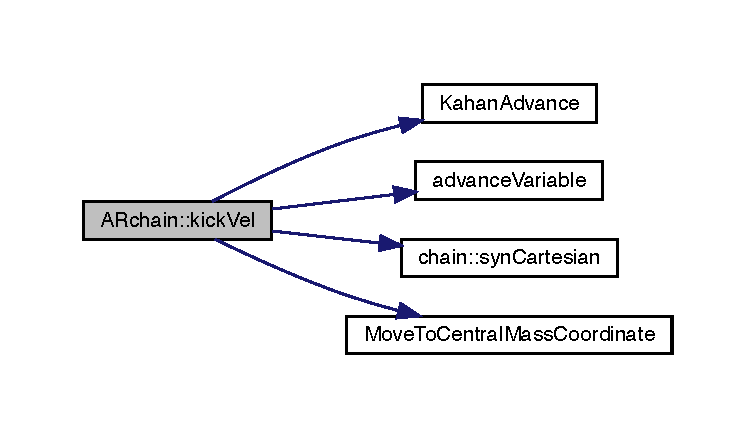
\includegraphics[width=350pt]{class_a_rchain_a0b073cd82321047d7fafda59cef998ef_cgraph}
\end{center}
\end{figure}
\mbox{\Hypertarget{class_a_rchain_a7edf1240a094d55df222c816659dced0}\label{class_a_rchain_a7edf1240a094d55df222c816659dced0}} 
\index{A\+Rchain@{A\+Rchain}!load@{load}}
\index{load@{load}!A\+Rchain@{A\+Rchain}}
\subsubsection{\texorpdfstring{load()}{load()}}
{\footnotesize\ttfamily template$<$typename Interaction , typename Evolved\+Data , typename Regularitor $>$ \\
void \mbox{\hyperlink{class_a_rchain}{A\+Rchain}}$<$ Interaction, Evolved\+Data, Regularitor $>$\+::load (\begin{DoxyParamCaption}\item[{\mbox{\hyperlink{class_a_rchain_a829aca51411c08ffd518294770a374d5}{Plain\+Array}} \&}]{data }\end{DoxyParamCaption})}

Here is the call graph for this function\+:
\nopagebreak
\begin{figure}[H]
\begin{center}
\leavevmode
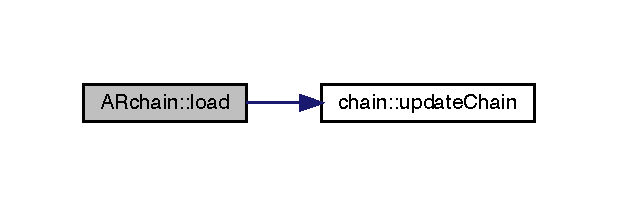
\includegraphics[width=296pt]{class_a_rchain_a7edf1240a094d55df222c816659dced0_cgraph}
\end{center}
\end{figure}
\mbox{\Hypertarget{class_a_rchain_a7bcc783f99cad1e9113d2b505544aba1}\label{class_a_rchain_a7bcc783f99cad1e9113d2b505544aba1}} 
\index{A\+Rchain@{A\+Rchain}!operator=@{operator=}}
\index{operator=@{operator=}!A\+Rchain@{A\+Rchain}}
\subsubsection{\texorpdfstring{operator=()}{operator=()}}
{\footnotesize\ttfamily template$<$typename Interaction , typename Evolved\+Data , typename Regularitor $>$ \\
const \mbox{\hyperlink{class_a_rchain}{A\+Rchain}}$<$ Interaction, Evolved\+Data, Regularitor $>$ \& \mbox{\hyperlink{class_a_rchain}{A\+Rchain}}$<$ Interaction, Evolved\+Data, Regularitor $>$\+::operator= (\begin{DoxyParamCaption}\item[{const \mbox{\hyperlink{class_a_rchain}{A\+Rchain}}$<$ Interaction, Evolved\+Data, Regularitor $>$ \&}]{other }\end{DoxyParamCaption})}

\mbox{\Hypertarget{class_a_rchain_a86bd89bacf59c9c3bb0594499db82e04}\label{class_a_rchain_a86bd89bacf59c9c3bb0594499db82e04}} 
\index{A\+Rchain@{A\+Rchain}!read@{read}}
\index{read@{read}!A\+Rchain@{A\+Rchain}}
\subsubsection{\texorpdfstring{read()}{read()}}
{\footnotesize\ttfamily template$<$typename Interaction , typename Evolved\+Data , typename Regularitor $>$ \\
std\+::istream \& \mbox{\hyperlink{class_a_rchain}{A\+Rchain}}$<$ Interaction, Evolved\+Data, Regularitor $>$\+::read (\begin{DoxyParamCaption}\item[{std\+::istream \&}]{input }\end{DoxyParamCaption})}

Here is the call graph for this function\+:
\nopagebreak
\begin{figure}[H]
\begin{center}
\leavevmode
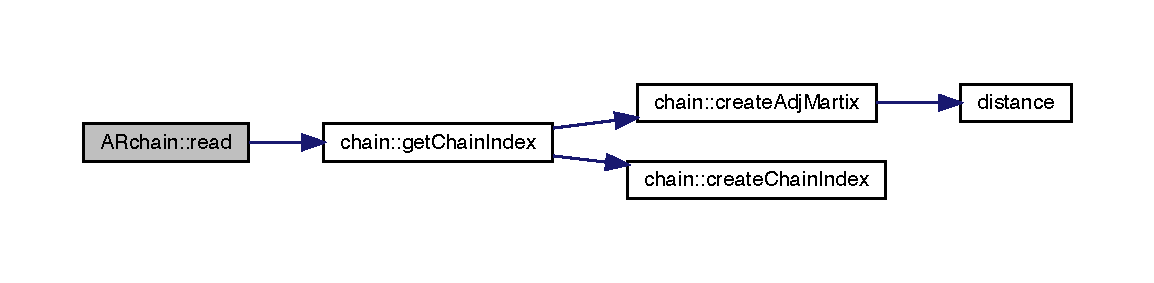
\includegraphics[width=350pt]{class_a_rchain_a86bd89bacf59c9c3bb0594499db82e04_cgraph}
\end{center}
\end{figure}
\mbox{\Hypertarget{class_a_rchain_ac612af46ce057d56dc47a6d28738a4cf}\label{class_a_rchain_ac612af46ce057d56dc47a6d28738a4cf}} 
\index{A\+Rchain@{A\+Rchain}!size@{size}}
\index{size@{size}!A\+Rchain@{A\+Rchain}}
\subsubsection{\texorpdfstring{size()}{size()}}
{\footnotesize\ttfamily template$<$typename Interaction, typename Evolved\+Data, typename Regularitor$>$ \\
static constexpr size\+\_\+t \mbox{\hyperlink{class_a_rchain}{A\+Rchain}}$<$ Interaction, Evolved\+Data, Regularitor $>$\+::size (\begin{DoxyParamCaption}{ }\end{DoxyParamCaption})\hspace{0.3cm}{\ttfamily [inline]}, {\ttfamily [static]}}

\mbox{\Hypertarget{class_a_rchain_a979a40abd086aeb411dc8e82a3bb1cdf}\label{class_a_rchain_a979a40abd086aeb411dc8e82a3bb1cdf}} 
\index{A\+Rchain@{A\+Rchain}!time\+Scale@{time\+Scale}}
\index{time\+Scale@{time\+Scale}!A\+Rchain@{A\+Rchain}}
\subsubsection{\texorpdfstring{time\+Scale()}{timeScale()}}
{\footnotesize\ttfamily template$<$typename Interaction , typename Evolved\+Data , typename Regularitor $>$ \\
Evolved\+Data\+::\+Scalar \mbox{\hyperlink{class_a_rchain}{A\+Rchain}}$<$ Interaction, Evolved\+Data, Regularitor $>$\+::time\+Scale (\begin{DoxyParamCaption}\item[{\mbox{\hyperlink{class_a_rchain_a707e42a79e4744424a34c9007e84ee07}{Scalar}}}]{scale }\end{DoxyParamCaption})}

\mbox{\Hypertarget{class_a_rchain_a92865bff07dc16e3065a8f695120a5f5}\label{class_a_rchain_a92865bff07dc16e3065a8f695120a5f5}} 
\index{A\+Rchain@{A\+Rchain}!update\+Acc\+With@{update\+Acc\+With}}
\index{update\+Acc\+With@{update\+Acc\+With}!A\+Rchain@{A\+Rchain}}
\subsubsection{\texorpdfstring{update\+Acc\+With()}{updateAccWith()}}
{\footnotesize\ttfamily template$<$typename Interaction , typename Evolved\+Data , typename Regularitor $>$ \\
void \mbox{\hyperlink{class_a_rchain}{A\+Rchain}}$<$ Interaction, Evolved\+Data, Regularitor $>$\+::update\+Acc\+With (\begin{DoxyParamCaption}\item[{\mbox{\hyperlink{class_a_rchain_a019fbadb9f4e5892736d9127537338bb}{Vector\+Array}} \&}]{vel,  }\item[{\mbox{\hyperlink{class_a_rchain_a019fbadb9f4e5892736d9127537338bb}{Vector\+Array}} \&}]{chain\+Vel }\end{DoxyParamCaption})\hspace{0.3cm}{\ttfamily [private]}}

\mbox{\Hypertarget{class_a_rchain_ad576df000b6d9f3948eae2793c6b3c54}\label{class_a_rchain_ad576df000b6d9f3948eae2793c6b3c54}} 
\index{A\+Rchain@{A\+Rchain}!update\+Chain@{update\+Chain}}
\index{update\+Chain@{update\+Chain}!A\+Rchain@{A\+Rchain}}
\subsubsection{\texorpdfstring{update\+Chain()}{updateChain()}}
{\footnotesize\ttfamily template$<$typename Interaction , typename Evolved\+Data , typename Regularitor $>$ \\
void \mbox{\hyperlink{class_a_rchain}{A\+Rchain}}$<$ Interaction, Evolved\+Data, Regularitor $>$\+::update\+Chain (\begin{DoxyParamCaption}{ }\end{DoxyParamCaption})\hspace{0.3cm}{\ttfamily [private]}}

Here is the call graph for this function\+:
\nopagebreak
\begin{figure}[H]
\begin{center}
\leavevmode
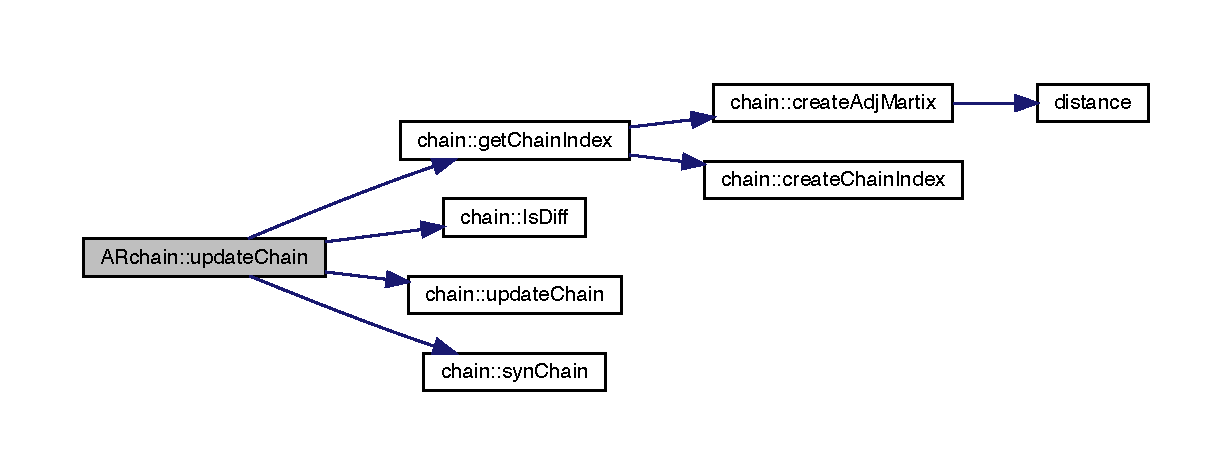
\includegraphics[width=350pt]{class_a_rchain_ad576df000b6d9f3948eae2793c6b3c54_cgraph}
\end{center}
\end{figure}
\mbox{\Hypertarget{class_a_rchain_a08ddf32fb537ac1556b2e4560abf3b5d}\label{class_a_rchain_a08ddf32fb537ac1556b2e4560abf3b5d}} 
\index{A\+Rchain@{A\+Rchain}!update\+Vel\+Indep\+Acc@{update\+Vel\+Indep\+Acc}}
\index{update\+Vel\+Indep\+Acc@{update\+Vel\+Indep\+Acc}!A\+Rchain@{A\+Rchain}}
\subsubsection{\texorpdfstring{update\+Vel\+Indep\+Acc()}{updateVelIndepAcc()}}
{\footnotesize\ttfamily template$<$typename Interaction , typename Evolved\+Data , typename Regularitor $>$ \\
void \mbox{\hyperlink{class_a_rchain}{A\+Rchain}}$<$ Interaction, Evolved\+Data, Regularitor $>$\+::update\+Vel\+Indep\+Acc (\begin{DoxyParamCaption}{ }\end{DoxyParamCaption})\hspace{0.3cm}{\ttfamily [private]}}



\subsection{Member Data Documentation}
\mbox{\Hypertarget{class_a_rchain_af7780024bfc1beca5f5622086b909db2}\label{class_a_rchain_af7780024bfc1beca5f5622086b909db2}} 
\index{A\+Rchain@{A\+Rchain}!chain@{chain}}
\index{chain@{chain}!A\+Rchain@{A\+Rchain}}
\subsubsection{\texorpdfstring{chain}{chain}}
{\footnotesize\ttfamily template$<$typename Interaction, typename Evolved\+Data, typename Regularitor$>$ \\
Evolved\+Data \mbox{\hyperlink{class_a_rchain}{A\+Rchain}}$<$ Interaction, Evolved\+Data, Regularitor $>$\+::chain\hspace{0.3cm}{\ttfamily [private]}}

\mbox{\Hypertarget{class_a_rchain_a0691e6612b661e329f1fc72d4cb7c895}\label{class_a_rchain_a0691e6612b661e329f1fc72d4cb7c895}} 
\index{A\+Rchain@{A\+Rchain}!chain\+Index@{chain\+Index}}
\index{chain\+Index@{chain\+Index}!A\+Rchain@{A\+Rchain}}
\subsubsection{\texorpdfstring{chain\+Index}{chainIndex}}
{\footnotesize\ttfamily template$<$typename Interaction, typename Evolved\+Data, typename Regularitor$>$ \\
\mbox{\hyperlink{class_a_rchain_aae40d4b5881eecfc960814f9e368215d}{Index\+Array}} \mbox{\hyperlink{class_a_rchain}{A\+Rchain}}$<$ Interaction, Evolved\+Data, Regularitor $>$\+::chain\+Index\hspace{0.3cm}{\ttfamily [private]}}

\mbox{\Hypertarget{class_a_rchain_a64087e0cb9cdb6b118b4a6e416d9f012}\label{class_a_rchain_a64087e0cb9cdb6b118b4a6e416d9f012}} 
\index{A\+Rchain@{A\+Rchain}!chain\+Vel\+Dep\+Acc@{chain\+Vel\+Dep\+Acc}}
\index{chain\+Vel\+Dep\+Acc@{chain\+Vel\+Dep\+Acc}!A\+Rchain@{A\+Rchain}}
\subsubsection{\texorpdfstring{chain\+Vel\+Dep\+Acc}{chainVelDepAcc}}
{\footnotesize\ttfamily template$<$typename Interaction, typename Evolved\+Data, typename Regularitor$>$ \\
\mbox{\hyperlink{class_a_rchain_a019fbadb9f4e5892736d9127537338bb}{Vector\+Array}} \mbox{\hyperlink{class_a_rchain}{A\+Rchain}}$<$ Interaction, Evolved\+Data, Regularitor $>$\+::chain\+Vel\+Dep\+Acc\hspace{0.3cm}{\ttfamily [private]}}

\mbox{\Hypertarget{class_a_rchain_a80d060a3341913f94c4bbbf2e2321b1d}\label{class_a_rchain_a80d060a3341913f94c4bbbf2e2321b1d}} 
\index{A\+Rchain@{A\+Rchain}!chain\+Vel\+Indep\+Acc@{chain\+Vel\+Indep\+Acc}}
\index{chain\+Vel\+Indep\+Acc@{chain\+Vel\+Indep\+Acc}!A\+Rchain@{A\+Rchain}}
\subsubsection{\texorpdfstring{chain\+Vel\+Indep\+Acc}{chainVelIndepAcc}}
{\footnotesize\ttfamily template$<$typename Interaction, typename Evolved\+Data, typename Regularitor$>$ \\
\mbox{\hyperlink{class_a_rchain_a019fbadb9f4e5892736d9127537338bb}{Vector\+Array}} \mbox{\hyperlink{class_a_rchain}{A\+Rchain}}$<$ Interaction, Evolved\+Data, Regularitor $>$\+::chain\+Vel\+Indep\+Acc\hspace{0.3cm}{\ttfamily [private]}}

\mbox{\Hypertarget{class_a_rchain_a4dd20aa56d6a6403260ad3ced2987eb0}\label{class_a_rchain_a4dd20aa56d6a6403260ad3ced2987eb0}} 
\index{A\+Rchain@{A\+Rchain}!regular@{regular}}
\index{regular@{regular}!A\+Rchain@{A\+Rchain}}
\subsubsection{\texorpdfstring{regular}{regular}}
{\footnotesize\ttfamily template$<$typename Interaction, typename Evolved\+Data, typename Regularitor$>$ \\
Regularitor \mbox{\hyperlink{class_a_rchain}{A\+Rchain}}$<$ Interaction, Evolved\+Data, Regularitor $>$\+::regular\hspace{0.3cm}{\ttfamily [private]}}

\mbox{\Hypertarget{class_a_rchain_a3c3a74f839bbfe5cbe1d8eb239dd8cc1}\label{class_a_rchain_a3c3a74f839bbfe5cbe1d8eb239dd8cc1}} 
\index{A\+Rchain@{A\+Rchain}!vel\+Dep\+Acc@{vel\+Dep\+Acc}}
\index{vel\+Dep\+Acc@{vel\+Dep\+Acc}!A\+Rchain@{A\+Rchain}}
\subsubsection{\texorpdfstring{vel\+Dep\+Acc}{velDepAcc}}
{\footnotesize\ttfamily template$<$typename Interaction, typename Evolved\+Data, typename Regularitor$>$ \\
\mbox{\hyperlink{class_a_rchain_a019fbadb9f4e5892736d9127537338bb}{Vector\+Array}} \mbox{\hyperlink{class_a_rchain}{A\+Rchain}}$<$ Interaction, Evolved\+Data, Regularitor $>$\+::vel\+Dep\+Acc\hspace{0.3cm}{\ttfamily [private]}}

\mbox{\Hypertarget{class_a_rchain_a5ad11cefbdb69a58225b799b36dd9eee}\label{class_a_rchain_a5ad11cefbdb69a58225b799b36dd9eee}} 
\index{A\+Rchain@{A\+Rchain}!vel\+Dep\+Force@{vel\+Dep\+Force}}
\index{vel\+Dep\+Force@{vel\+Dep\+Force}!A\+Rchain@{A\+Rchain}}
\subsubsection{\texorpdfstring{vel\+Dep\+Force}{velDepForce}}
{\footnotesize\ttfamily template$<$typename Interaction, typename Evolved\+Data, typename Regularitor$>$ \\
Interaction \mbox{\hyperlink{class_a_rchain}{A\+Rchain}}$<$ Interaction, Evolved\+Data, Regularitor $>$\+::vel\+Dep\+Force\hspace{0.3cm}{\ttfamily [private]}}

\mbox{\Hypertarget{class_a_rchain_a9359b4fb9f08ad849b0f1dfbdf661016}\label{class_a_rchain_a9359b4fb9f08ad849b0f1dfbdf661016}} 
\index{A\+Rchain@{A\+Rchain}!vel\+Indep\+Acc@{vel\+Indep\+Acc}}
\index{vel\+Indep\+Acc@{vel\+Indep\+Acc}!A\+Rchain@{A\+Rchain}}
\subsubsection{\texorpdfstring{vel\+Indep\+Acc}{velIndepAcc}}
{\footnotesize\ttfamily template$<$typename Interaction, typename Evolved\+Data, typename Regularitor$>$ \\
\mbox{\hyperlink{class_a_rchain_a019fbadb9f4e5892736d9127537338bb}{Vector\+Array}} \mbox{\hyperlink{class_a_rchain}{A\+Rchain}}$<$ Interaction, Evolved\+Data, Regularitor $>$\+::vel\+Indep\+Acc\hspace{0.3cm}{\ttfamily [private]}}



The documentation for this class was generated from the following file\+:\begin{DoxyCompactItemize}
\item 
particle\+System/\mbox{\hyperlink{_a_rchain_8h}{A\+Rchain.\+h}}\end{DoxyCompactItemize}

\hypertarget{class_a_rchain_3_01_newtonian_3_01typename_01_evolved_data_1_1_scalar_01_4_00_01_evolved_data_00_01_regularitor_01_4}{}\subsection{A\+Rchain$<$ Newtonian$<$ typename Evolved\+Data\+:\+:Scalar $>$, Evolved\+Data, Regularitor $>$ Class Template Reference}
\label{class_a_rchain_3_01_newtonian_3_01typename_01_evolved_data_1_1_scalar_01_4_00_01_evolved_data_00_01_regularitor_01_4}\index{A\+Rchain$<$ Newtonian$<$ typename Evolved\+Data\+::\+Scalar $>$, Evolved\+Data, Regularitor $>$@{A\+Rchain$<$ Newtonian$<$ typename Evolved\+Data\+::\+Scalar $>$, Evolved\+Data, Regularitor $>$}}


Partial specilization of template \mbox{\hyperlink{class_a_rchain}{A\+Rchain}}.  




{\ttfamily \#include $<$A\+Rchain.\+h$>$}



Inheritance diagram for A\+Rchain$<$ Newtonian$<$ typename Evolved\+Data\+:\+:Scalar $>$, Evolved\+Data, Regularitor $>$\+:\nopagebreak
\begin{figure}[H]
\begin{center}
\leavevmode
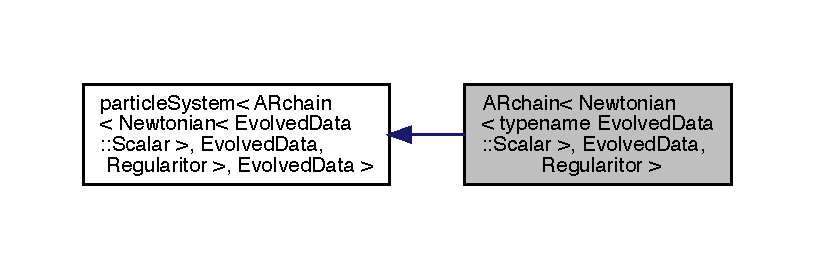
\includegraphics[width=350pt]{class_a_rchain_3_01_newtonian_3_01typename_01_evolved_data_1_1_scalar_01_4_00_01_evolved_data_009697bd28ff0e21ae1fe098221d830f5f}
\end{center}
\end{figure}


Collaboration diagram for A\+Rchain$<$ Newtonian$<$ typename Evolved\+Data\+:\+:Scalar $>$, Evolved\+Data, Regularitor $>$\+:\nopagebreak
\begin{figure}[H]
\begin{center}
\leavevmode
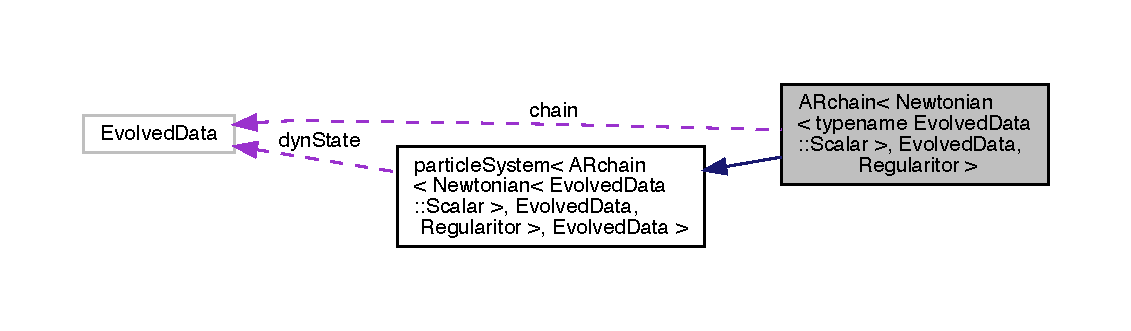
\includegraphics[width=350pt]{class_a_rchain_3_01_newtonian_3_01typename_01_evolved_data_1_1_scalar_01_4_00_01_evolved_data_0008f198c2eb8c667ccc6c16f5130b7c81}
\end{center}
\end{figure}
\subsubsection*{Public Types}
\begin{DoxyCompactItemize}
\item 
typedef Evolved\+Data\+::\+Scalar \mbox{\hyperlink{class_a_rchain_3_01_newtonian_3_01typename_01_evolved_data_1_1_scalar_01_4_00_01_evolved_data_00_01_regularitor_01_4_a2c77dc1b58a25ac5c6ee95dd7809f693}{Scalar}}
\item 
typedef Evolved\+Data\+::\+Vector \mbox{\hyperlink{class_a_rchain_3_01_newtonian_3_01typename_01_evolved_data_1_1_scalar_01_4_00_01_evolved_data_00_01_regularitor_01_4_a0adb648f04fbe3ba3a0289376b56a9e1}{Vector}}
\item 
typedef Evolved\+Data\+::\+Vector\+Array \mbox{\hyperlink{class_a_rchain_3_01_newtonian_3_01typename_01_evolved_data_1_1_scalar_01_4_00_01_evolved_data_00_01_regularitor_01_4_a1ff7d2e64f488df9edae2ad796945bbd}{Vector\+Array}}
\item 
typedef Evolved\+Data\+::\+Scalar\+Array \mbox{\hyperlink{class_a_rchain_3_01_newtonian_3_01typename_01_evolved_data_1_1_scalar_01_4_00_01_evolved_data_00_01_regularitor_01_4_a65b11346d3c11858344b450f2247afd9}{Scalar\+Array}}
\item 
typedef \mbox{\hyperlink{class_a_rchain_aeb4d9b0a28ae3b4e4286edf838e5a905}{std\+::array}}$<$ size\+\_\+t, \mbox{\hyperlink{class_a_rchain_ac612af46ce057d56dc47a6d28738a4cf}{Evolved\+Data\+::size}}()$>$ \mbox{\hyperlink{class_a_rchain_3_01_newtonian_3_01typename_01_evolved_data_1_1_scalar_01_4_00_01_evolved_data_00_01_regularitor_01_4_a0072f8585c3e6ba8d64cb81be90fb376}{Index\+Array}}
\item 
typedef \mbox{\hyperlink{class_a_rchain_aeb4d9b0a28ae3b4e4286edf838e5a905}{std\+::array}}$<$ \mbox{\hyperlink{class_a_rchain_3_01_newtonian_3_01typename_01_evolved_data_1_1_scalar_01_4_00_01_evolved_data_00_01_regularitor_01_4_a2c77dc1b58a25ac5c6ee95dd7809f693}{Scalar}}, \mbox{\hyperlink{classparticle_system_aac9e6701e4486c89b508a2508b77089b}{Evolved\+Data\+::volume}}()$>$ \mbox{\hyperlink{class_a_rchain_3_01_newtonian_3_01typename_01_evolved_data_1_1_scalar_01_4_00_01_evolved_data_00_01_regularitor_01_4_a8cf940df8dabb6c78662f839c2b13c9a}{Plain\+Array}}
\end{DoxyCompactItemize}
\subsubsection*{Public Member Functions}
\begin{DoxyCompactItemize}
\item 
void \mbox{\hyperlink{class_a_rchain_3_01_newtonian_3_01typename_01_evolved_data_1_1_scalar_01_4_00_01_evolved_data_00_01_regularitor_01_4_adffd5a74134d2a87e4f07908ea5beef4}{advance\+Pos}} (\mbox{\hyperlink{class_a_rchain_3_01_newtonian_3_01typename_01_evolved_data_1_1_scalar_01_4_00_01_evolved_data_00_01_regularitor_01_4_a2c77dc1b58a25ac5c6ee95dd7809f693}{Scalar}} time\+Step\+Size)
\begin{DoxyCompactList}\small\item\em Advance position one step with current velocity. \end{DoxyCompactList}\item 
void \mbox{\hyperlink{class_a_rchain_3_01_newtonian_3_01typename_01_evolved_data_1_1_scalar_01_4_00_01_evolved_data_00_01_regularitor_01_4_ad11d21617228157e755aa334d9c621a7}{advance\+Vel}} (\mbox{\hyperlink{class_a_rchain_3_01_newtonian_3_01typename_01_evolved_data_1_1_scalar_01_4_00_01_evolved_data_00_01_regularitor_01_4_a2c77dc1b58a25ac5c6ee95dd7809f693}{Scalar}} time\+Step\+Size)
\begin{DoxyCompactList}\small\item\em Advance velocity one step with current acceleration. \end{DoxyCompactList}\item 
const \mbox{\hyperlink{class_a_rchain}{A\+Rchain}} \& \mbox{\hyperlink{class_a_rchain_3_01_newtonian_3_01typename_01_evolved_data_1_1_scalar_01_4_00_01_evolved_data_00_01_regularitor_01_4_a577ecdf4e934627257a0824d59404831}{operator=}} (const \mbox{\hyperlink{class_a_rchain}{A\+Rchain}} \&other)
\begin{DoxyCompactList}\small\item\em Overload operator =. \end{DoxyCompactList}\item 
std\+::istream \& \mbox{\hyperlink{class_a_rchain_3_01_newtonian_3_01typename_01_evolved_data_1_1_scalar_01_4_00_01_evolved_data_00_01_regularitor_01_4_aa4b0a64e05c3942e402606e74c08b593}{read}} (std\+::istream \&)
\begin{DoxyCompactList}\small\item\em Input data from standard c++ istream. \end{DoxyCompactList}\item 
void \mbox{\hyperlink{class_a_rchain_3_01_newtonian_3_01typename_01_evolved_data_1_1_scalar_01_4_00_01_evolved_data_00_01_regularitor_01_4_a8e7bc5b32dbd7a0c9c3541f17fa54e28}{load}} (\mbox{\hyperlink{class_a_rchain_3_01_newtonian_3_01typename_01_evolved_data_1_1_scalar_01_4_00_01_evolved_data_00_01_regularitor_01_4_a8cf940df8dabb6c78662f839c2b13c9a}{Plain\+Array}} \&data)
\begin{DoxyCompactList}\small\item\em Load data from a plain array. \end{DoxyCompactList}\item 
\mbox{\hyperlink{class_a_rchain_3_01_newtonian_3_01typename_01_evolved_data_1_1_scalar_01_4_00_01_evolved_data_00_01_regularitor_01_4_a2c77dc1b58a25ac5c6ee95dd7809f693}{Scalar}} \mbox{\hyperlink{class_a_rchain_3_01_newtonian_3_01typename_01_evolved_data_1_1_scalar_01_4_00_01_evolved_data_00_01_regularitor_01_4_aa7aadb0b5ffcfebc759e4f091c4fc763}{time\+Scale}} (\mbox{\hyperlink{class_a_rchain_3_01_newtonian_3_01typename_01_evolved_data_1_1_scalar_01_4_00_01_evolved_data_00_01_regularitor_01_4_a2c77dc1b58a25ac5c6ee95dd7809f693}{Scalar}} scale)
\begin{DoxyCompactList}\small\item\em Interface to rescale the time. \end{DoxyCompactList}\item 
\mbox{\hyperlink{class_a_rchain_3_01_newtonian_3_01typename_01_evolved_data_1_1_scalar_01_4_00_01_evolved_data_00_01_regularitor_01_4_a8cf940df8dabb6c78662f839c2b13c9a}{Plain\+Array}} \& \mbox{\hyperlink{class_a_rchain_3_01_newtonian_3_01typename_01_evolved_data_1_1_scalar_01_4_00_01_evolved_data_00_01_regularitor_01_4_a919d200a913f75719c7240c030b9b113}{array}} ()
\begin{DoxyCompactList}\small\item\em Transfer the evolved data to a plain scalar array. \end{DoxyCompactList}\end{DoxyCompactItemize}
\subsubsection*{Static Public Member Functions}
\begin{DoxyCompactItemize}
\item 
static constexpr size\+\_\+t \mbox{\hyperlink{class_a_rchain_3_01_newtonian_3_01typename_01_evolved_data_1_1_scalar_01_4_00_01_evolved_data_00_01_regularitor_01_4_a928601b10d9a9e5ab02f36cf11efa263}{size}} ()
\begin{DoxyCompactList}\small\item\em Get the number of the particles. \end{DoxyCompactList}\end{DoxyCompactItemize}
\subsubsection*{Private Member Functions}
\begin{DoxyCompactItemize}
\item 
void \mbox{\hyperlink{class_a_rchain_3_01_newtonian_3_01typename_01_evolved_data_1_1_scalar_01_4_00_01_evolved_data_00_01_regularitor_01_4_a8427d55e9b05fca4a1db2b9024940e06}{advance\+Omega}} (\mbox{\hyperlink{class_a_rchain_3_01_newtonian_3_01typename_01_evolved_data_1_1_scalar_01_4_00_01_evolved_data_00_01_regularitor_01_4_a2c77dc1b58a25ac5c6ee95dd7809f693}{Scalar}} step\+Size)
\begin{DoxyCompactList}\small\item\em Advance regularization variable omega. \end{DoxyCompactList}\item 
void \mbox{\hyperlink{class_a_rchain_3_01_newtonian_3_01typename_01_evolved_data_1_1_scalar_01_4_00_01_evolved_data_00_01_regularitor_01_4_a2b11ca856564416ed6727c716ed284a8}{update\+Vel\+Indep\+Acc}} ()
\begin{DoxyCompactList}\small\item\em Update velocity independent acceleration. \end{DoxyCompactList}\item 
void \mbox{\hyperlink{class_a_rchain_3_01_newtonian_3_01typename_01_evolved_data_1_1_scalar_01_4_00_01_evolved_data_00_01_regularitor_01_4_acbe31e9aa918e4f80a2763e16f0bb7bc}{update\+Chain}} ()
\begin{DoxyCompactList}\small\item\em Update the chain data based on current Cartesian coordinates. \end{DoxyCompactList}\end{DoxyCompactItemize}
\subsubsection*{Private Attributes}
\begin{DoxyCompactItemize}
\item 
Evolved\+Data \mbox{\hyperlink{class_a_rchain_3_01_newtonian_3_01typename_01_evolved_data_1_1_scalar_01_4_00_01_evolved_data_00_01_regularitor_01_4_a39576accb53257bdb1b55e6d21acdf0f}{chain}}
\begin{DoxyCompactList}\small\item\em Evolved variables in chain coordinates. \end{DoxyCompactList}\item 
\mbox{\hyperlink{class_a_rchain_3_01_newtonian_3_01typename_01_evolved_data_1_1_scalar_01_4_00_01_evolved_data_00_01_regularitor_01_4_a0072f8585c3e6ba8d64cb81be90fb376}{Index\+Array}} \mbox{\hyperlink{class_a_rchain_3_01_newtonian_3_01typename_01_evolved_data_1_1_scalar_01_4_00_01_evolved_data_00_01_regularitor_01_4_a6a8ef156105e2f80dc143606d4ba10c9}{chain\+Index}}
\begin{DoxyCompactList}\small\item\em Mapping index from Cartesian coordinates to chain coordinates. \end{DoxyCompactList}\item 
\mbox{\hyperlink{class_a_rchain_3_01_newtonian_3_01typename_01_evolved_data_1_1_scalar_01_4_00_01_evolved_data_00_01_regularitor_01_4_a1ff7d2e64f488df9edae2ad796945bbd}{Vector\+Array}} \mbox{\hyperlink{class_a_rchain_3_01_newtonian_3_01typename_01_evolved_data_1_1_scalar_01_4_00_01_evolved_data_00_01_regularitor_01_4_af0862cdda12b7ba2ba5d5d098d008398}{vel\+Indep\+Acc}}
\begin{DoxyCompactList}\small\item\em Velocity independent acceleration array in Cartesian coordiantes. \end{DoxyCompactList}\item 
Regularitor \mbox{\hyperlink{class_a_rchain_3_01_newtonian_3_01typename_01_evolved_data_1_1_scalar_01_4_00_01_evolved_data_00_01_regularitor_01_4_a6e5a31aa07620ab9f3503ebc412ff969}{regular}}
\begin{DoxyCompactList}\small\item\em Regularization interface. \end{DoxyCompactList}\end{DoxyCompactItemize}
\subsubsection*{Additional Inherited Members}


\subsubsection{Detailed Description}
\subsubsection*{template$<$typename Evolved\+Data, typename Regularitor$>$\newline
class A\+Rchain$<$ Newtonian$<$ typename Evolved\+Data\+::\+Scalar $>$, Evolved\+Data, Regularitor $>$}

Partial specilization of template \mbox{\hyperlink{class_a_rchain}{A\+Rchain}}. 

\subsubsection{Member Typedef Documentation}
\mbox{\Hypertarget{class_a_rchain_3_01_newtonian_3_01typename_01_evolved_data_1_1_scalar_01_4_00_01_evolved_data_00_01_regularitor_01_4_a0072f8585c3e6ba8d64cb81be90fb376}\label{class_a_rchain_3_01_newtonian_3_01typename_01_evolved_data_1_1_scalar_01_4_00_01_evolved_data_00_01_regularitor_01_4_a0072f8585c3e6ba8d64cb81be90fb376}} 
\index{A\+Rchain$<$ Newtonian$<$ typename Evolved\+Data\+::\+Scalar $>$, Evolved\+Data, Regularitor $>$@{A\+Rchain$<$ Newtonian$<$ typename Evolved\+Data\+::\+Scalar $>$, Evolved\+Data, Regularitor $>$}!Index\+Array@{Index\+Array}}
\index{Index\+Array@{Index\+Array}!A\+Rchain$<$ Newtonian$<$ typename Evolved\+Data\+::\+Scalar $>$, Evolved\+Data, Regularitor $>$@{A\+Rchain$<$ Newtonian$<$ typename Evolved\+Data\+::\+Scalar $>$, Evolved\+Data, Regularitor $>$}}
\paragraph{\texorpdfstring{Index\+Array}{IndexArray}}
{\footnotesize\ttfamily template$<$typename Evolved\+Data , typename Regularitor $>$ \\
typedef \mbox{\hyperlink{class_a_rchain_aeb4d9b0a28ae3b4e4286edf838e5a905}{std\+::array}}$<$size\+\_\+t, \mbox{\hyperlink{class_a_rchain_ac612af46ce057d56dc47a6d28738a4cf}{Evolved\+Data\+::size}}()$>$ \mbox{\hyperlink{class_a_rchain}{A\+Rchain}}$<$ \mbox{\hyperlink{class_newtonian}{Newtonian}}$<$ typename \mbox{\hyperlink{class_a_rchain_a707e42a79e4744424a34c9007e84ee07}{Evolved\+Data\+::\+Scalar}} $>$, Evolved\+Data, Regularitor $>$\+::\mbox{\hyperlink{class_a_rchain_3_01_newtonian_3_01typename_01_evolved_data_1_1_scalar_01_4_00_01_evolved_data_00_01_regularitor_01_4_a0072f8585c3e6ba8d64cb81be90fb376}{Index\+Array}}}

\mbox{\Hypertarget{class_a_rchain_3_01_newtonian_3_01typename_01_evolved_data_1_1_scalar_01_4_00_01_evolved_data_00_01_regularitor_01_4_a8cf940df8dabb6c78662f839c2b13c9a}\label{class_a_rchain_3_01_newtonian_3_01typename_01_evolved_data_1_1_scalar_01_4_00_01_evolved_data_00_01_regularitor_01_4_a8cf940df8dabb6c78662f839c2b13c9a}} 
\index{A\+Rchain$<$ Newtonian$<$ typename Evolved\+Data\+::\+Scalar $>$, Evolved\+Data, Regularitor $>$@{A\+Rchain$<$ Newtonian$<$ typename Evolved\+Data\+::\+Scalar $>$, Evolved\+Data, Regularitor $>$}!Plain\+Array@{Plain\+Array}}
\index{Plain\+Array@{Plain\+Array}!A\+Rchain$<$ Newtonian$<$ typename Evolved\+Data\+::\+Scalar $>$, Evolved\+Data, Regularitor $>$@{A\+Rchain$<$ Newtonian$<$ typename Evolved\+Data\+::\+Scalar $>$, Evolved\+Data, Regularitor $>$}}
\paragraph{\texorpdfstring{Plain\+Array}{PlainArray}}
{\footnotesize\ttfamily template$<$typename Evolved\+Data , typename Regularitor $>$ \\
typedef \mbox{\hyperlink{class_a_rchain_aeb4d9b0a28ae3b4e4286edf838e5a905}{std\+::array}}$<$\mbox{\hyperlink{class_a_rchain_3_01_newtonian_3_01typename_01_evolved_data_1_1_scalar_01_4_00_01_evolved_data_00_01_regularitor_01_4_a2c77dc1b58a25ac5c6ee95dd7809f693}{Scalar}}, \mbox{\hyperlink{classparticle_system_aac9e6701e4486c89b508a2508b77089b}{Evolved\+Data\+::volume}}()$>$ \mbox{\hyperlink{class_a_rchain}{A\+Rchain}}$<$ \mbox{\hyperlink{class_newtonian}{Newtonian}}$<$ typename \mbox{\hyperlink{class_a_rchain_a707e42a79e4744424a34c9007e84ee07}{Evolved\+Data\+::\+Scalar}} $>$, Evolved\+Data, Regularitor $>$\+::\mbox{\hyperlink{class_a_rchain_3_01_newtonian_3_01typename_01_evolved_data_1_1_scalar_01_4_00_01_evolved_data_00_01_regularitor_01_4_a8cf940df8dabb6c78662f839c2b13c9a}{Plain\+Array}}}

\mbox{\Hypertarget{class_a_rchain_3_01_newtonian_3_01typename_01_evolved_data_1_1_scalar_01_4_00_01_evolved_data_00_01_regularitor_01_4_a2c77dc1b58a25ac5c6ee95dd7809f693}\label{class_a_rchain_3_01_newtonian_3_01typename_01_evolved_data_1_1_scalar_01_4_00_01_evolved_data_00_01_regularitor_01_4_a2c77dc1b58a25ac5c6ee95dd7809f693}} 
\index{A\+Rchain$<$ Newtonian$<$ typename Evolved\+Data\+::\+Scalar $>$, Evolved\+Data, Regularitor $>$@{A\+Rchain$<$ Newtonian$<$ typename Evolved\+Data\+::\+Scalar $>$, Evolved\+Data, Regularitor $>$}!Scalar@{Scalar}}
\index{Scalar@{Scalar}!A\+Rchain$<$ Newtonian$<$ typename Evolved\+Data\+::\+Scalar $>$, Evolved\+Data, Regularitor $>$@{A\+Rchain$<$ Newtonian$<$ typename Evolved\+Data\+::\+Scalar $>$, Evolved\+Data, Regularitor $>$}}
\paragraph{\texorpdfstring{Scalar}{Scalar}}
{\footnotesize\ttfamily template$<$typename Evolved\+Data , typename Regularitor $>$ \\
typedef Evolved\+Data\+::\+Scalar \mbox{\hyperlink{class_a_rchain}{A\+Rchain}}$<$ \mbox{\hyperlink{class_newtonian}{Newtonian}}$<$ typename Evolved\+Data\+::\+Scalar $>$, Evolved\+Data, Regularitor $>$\+::\mbox{\hyperlink{class_a_rchain_3_01_newtonian_3_01typename_01_evolved_data_1_1_scalar_01_4_00_01_evolved_data_00_01_regularitor_01_4_a2c77dc1b58a25ac5c6ee95dd7809f693}{Scalar}}}

\mbox{\Hypertarget{class_a_rchain_3_01_newtonian_3_01typename_01_evolved_data_1_1_scalar_01_4_00_01_evolved_data_00_01_regularitor_01_4_a65b11346d3c11858344b450f2247afd9}\label{class_a_rchain_3_01_newtonian_3_01typename_01_evolved_data_1_1_scalar_01_4_00_01_evolved_data_00_01_regularitor_01_4_a65b11346d3c11858344b450f2247afd9}} 
\index{A\+Rchain$<$ Newtonian$<$ typename Evolved\+Data\+::\+Scalar $>$, Evolved\+Data, Regularitor $>$@{A\+Rchain$<$ Newtonian$<$ typename Evolved\+Data\+::\+Scalar $>$, Evolved\+Data, Regularitor $>$}!Scalar\+Array@{Scalar\+Array}}
\index{Scalar\+Array@{Scalar\+Array}!A\+Rchain$<$ Newtonian$<$ typename Evolved\+Data\+::\+Scalar $>$, Evolved\+Data, Regularitor $>$@{A\+Rchain$<$ Newtonian$<$ typename Evolved\+Data\+::\+Scalar $>$, Evolved\+Data, Regularitor $>$}}
\paragraph{\texorpdfstring{Scalar\+Array}{ScalarArray}}
{\footnotesize\ttfamily template$<$typename Evolved\+Data , typename Regularitor $>$ \\
typedef Evolved\+Data\+::\+Scalar\+Array \mbox{\hyperlink{class_a_rchain}{A\+Rchain}}$<$ \mbox{\hyperlink{class_newtonian}{Newtonian}}$<$ typename \mbox{\hyperlink{class_a_rchain_a707e42a79e4744424a34c9007e84ee07}{Evolved\+Data\+::\+Scalar}} $>$, Evolved\+Data, Regularitor $>$\+::\mbox{\hyperlink{class_a_rchain_3_01_newtonian_3_01typename_01_evolved_data_1_1_scalar_01_4_00_01_evolved_data_00_01_regularitor_01_4_a65b11346d3c11858344b450f2247afd9}{Scalar\+Array}}}

\mbox{\Hypertarget{class_a_rchain_3_01_newtonian_3_01typename_01_evolved_data_1_1_scalar_01_4_00_01_evolved_data_00_01_regularitor_01_4_a0adb648f04fbe3ba3a0289376b56a9e1}\label{class_a_rchain_3_01_newtonian_3_01typename_01_evolved_data_1_1_scalar_01_4_00_01_evolved_data_00_01_regularitor_01_4_a0adb648f04fbe3ba3a0289376b56a9e1}} 
\index{A\+Rchain$<$ Newtonian$<$ typename Evolved\+Data\+::\+Scalar $>$, Evolved\+Data, Regularitor $>$@{A\+Rchain$<$ Newtonian$<$ typename Evolved\+Data\+::\+Scalar $>$, Evolved\+Data, Regularitor $>$}!Vector@{Vector}}
\index{Vector@{Vector}!A\+Rchain$<$ Newtonian$<$ typename Evolved\+Data\+::\+Scalar $>$, Evolved\+Data, Regularitor $>$@{A\+Rchain$<$ Newtonian$<$ typename Evolved\+Data\+::\+Scalar $>$, Evolved\+Data, Regularitor $>$}}
\paragraph{\texorpdfstring{Vector}{Vector}}
{\footnotesize\ttfamily template$<$typename Evolved\+Data , typename Regularitor $>$ \\
typedef Evolved\+Data\+::\+Vector \mbox{\hyperlink{class_a_rchain}{A\+Rchain}}$<$ \mbox{\hyperlink{class_newtonian}{Newtonian}}$<$ typename \mbox{\hyperlink{class_a_rchain_a707e42a79e4744424a34c9007e84ee07}{Evolved\+Data\+::\+Scalar}} $>$, Evolved\+Data, Regularitor $>$\+::\mbox{\hyperlink{class_a_rchain_3_01_newtonian_3_01typename_01_evolved_data_1_1_scalar_01_4_00_01_evolved_data_00_01_regularitor_01_4_a0adb648f04fbe3ba3a0289376b56a9e1}{Vector}}}

\mbox{\Hypertarget{class_a_rchain_3_01_newtonian_3_01typename_01_evolved_data_1_1_scalar_01_4_00_01_evolved_data_00_01_regularitor_01_4_a1ff7d2e64f488df9edae2ad796945bbd}\label{class_a_rchain_3_01_newtonian_3_01typename_01_evolved_data_1_1_scalar_01_4_00_01_evolved_data_00_01_regularitor_01_4_a1ff7d2e64f488df9edae2ad796945bbd}} 
\index{A\+Rchain$<$ Newtonian$<$ typename Evolved\+Data\+::\+Scalar $>$, Evolved\+Data, Regularitor $>$@{A\+Rchain$<$ Newtonian$<$ typename Evolved\+Data\+::\+Scalar $>$, Evolved\+Data, Regularitor $>$}!Vector\+Array@{Vector\+Array}}
\index{Vector\+Array@{Vector\+Array}!A\+Rchain$<$ Newtonian$<$ typename Evolved\+Data\+::\+Scalar $>$, Evolved\+Data, Regularitor $>$@{A\+Rchain$<$ Newtonian$<$ typename Evolved\+Data\+::\+Scalar $>$, Evolved\+Data, Regularitor $>$}}
\paragraph{\texorpdfstring{Vector\+Array}{VectorArray}}
{\footnotesize\ttfamily template$<$typename Evolved\+Data , typename Regularitor $>$ \\
typedef Evolved\+Data\+::\+Vector\+Array \mbox{\hyperlink{class_a_rchain}{A\+Rchain}}$<$ \mbox{\hyperlink{class_newtonian}{Newtonian}}$<$ typename \mbox{\hyperlink{class_a_rchain_a707e42a79e4744424a34c9007e84ee07}{Evolved\+Data\+::\+Scalar}} $>$, Evolved\+Data, Regularitor $>$\+::\mbox{\hyperlink{class_a_rchain_3_01_newtonian_3_01typename_01_evolved_data_1_1_scalar_01_4_00_01_evolved_data_00_01_regularitor_01_4_a1ff7d2e64f488df9edae2ad796945bbd}{Vector\+Array}}}



\subsubsection{Member Function Documentation}
\mbox{\Hypertarget{class_a_rchain_3_01_newtonian_3_01typename_01_evolved_data_1_1_scalar_01_4_00_01_evolved_data_00_01_regularitor_01_4_a8427d55e9b05fca4a1db2b9024940e06}\label{class_a_rchain_3_01_newtonian_3_01typename_01_evolved_data_1_1_scalar_01_4_00_01_evolved_data_00_01_regularitor_01_4_a8427d55e9b05fca4a1db2b9024940e06}} 
\index{A\+Rchain$<$ Newtonian$<$ typename Evolved\+Data\+::\+Scalar $>$, Evolved\+Data, Regularitor $>$@{A\+Rchain$<$ Newtonian$<$ typename Evolved\+Data\+::\+Scalar $>$, Evolved\+Data, Regularitor $>$}!advance\+Omega@{advance\+Omega}}
\index{advance\+Omega@{advance\+Omega}!A\+Rchain$<$ Newtonian$<$ typename Evolved\+Data\+::\+Scalar $>$, Evolved\+Data, Regularitor $>$@{A\+Rchain$<$ Newtonian$<$ typename Evolved\+Data\+::\+Scalar $>$, Evolved\+Data, Regularitor $>$}}
\paragraph{\texorpdfstring{advance\+Omega()}{advanceOmega()}}
{\footnotesize\ttfamily template$<$typename Evolved\+Data , typename Regularitor $>$ \\
void \mbox{\hyperlink{class_a_rchain}{A\+Rchain}}$<$ \mbox{\hyperlink{class_newtonian}{Newtonian}}$<$ typename \mbox{\hyperlink{class_a_rchain_a707e42a79e4744424a34c9007e84ee07}{Evolved\+Data\+::\+Scalar}} $>$, Evolved\+Data, Regularitor $>$\+::advance\+Omega (\begin{DoxyParamCaption}\item[{\mbox{\hyperlink{class_a_rchain_3_01_newtonian_3_01typename_01_evolved_data_1_1_scalar_01_4_00_01_evolved_data_00_01_regularitor_01_4_a2c77dc1b58a25ac5c6ee95dd7809f693}{Scalar}}}]{step\+Size }\end{DoxyParamCaption})\hspace{0.3cm}{\ttfamily [private]}}



Advance regularization variable omega. 

Advance omega with velocity independent acceleration and velocity with physical time step size. 
\begin{DoxyParams}{Parameters}
{\em step\+Size} & Physical time step. \\
\hline
\end{DoxyParams}
\begin{DoxyNote}{Note}
Update the omega in chain, which will be processed by the integrator. 
\end{DoxyNote}
Here is the call graph for this function\+:\nopagebreak
\begin{figure}[H]
\begin{center}
\leavevmode
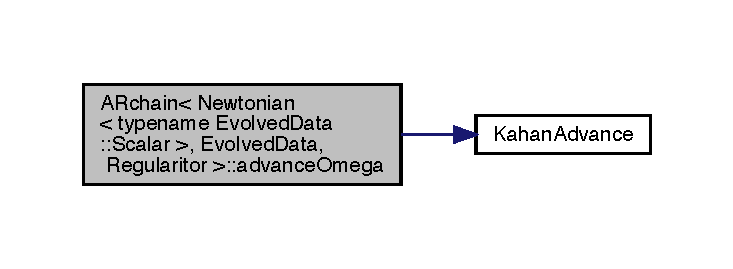
\includegraphics[width=350pt]{class_a_rchain_3_01_newtonian_3_01typename_01_evolved_data_1_1_scalar_01_4_00_01_evolved_data_00_01_regularitor_01_4_a8427d55e9b05fca4a1db2b9024940e06_cgraph}
\end{center}
\end{figure}
\mbox{\Hypertarget{class_a_rchain_3_01_newtonian_3_01typename_01_evolved_data_1_1_scalar_01_4_00_01_evolved_data_00_01_regularitor_01_4_adffd5a74134d2a87e4f07908ea5beef4}\label{class_a_rchain_3_01_newtonian_3_01typename_01_evolved_data_1_1_scalar_01_4_00_01_evolved_data_00_01_regularitor_01_4_adffd5a74134d2a87e4f07908ea5beef4}} 
\index{A\+Rchain$<$ Newtonian$<$ typename Evolved\+Data\+::\+Scalar $>$, Evolved\+Data, Regularitor $>$@{A\+Rchain$<$ Newtonian$<$ typename Evolved\+Data\+::\+Scalar $>$, Evolved\+Data, Regularitor $>$}!advance\+Pos@{advance\+Pos}}
\index{advance\+Pos@{advance\+Pos}!A\+Rchain$<$ Newtonian$<$ typename Evolved\+Data\+::\+Scalar $>$, Evolved\+Data, Regularitor $>$@{A\+Rchain$<$ Newtonian$<$ typename Evolved\+Data\+::\+Scalar $>$, Evolved\+Data, Regularitor $>$}}
\paragraph{\texorpdfstring{advance\+Pos()}{advancePos()}}
{\footnotesize\ttfamily template$<$typename Evolved\+Data , typename Regularitor $>$ \\
void \mbox{\hyperlink{class_a_rchain}{A\+Rchain}}$<$ \mbox{\hyperlink{class_newtonian}{Newtonian}}$<$ typename \mbox{\hyperlink{class_a_rchain_a707e42a79e4744424a34c9007e84ee07}{Evolved\+Data\+::\+Scalar}} $>$, Evolved\+Data, Regularitor $>$\+::advance\+Pos (\begin{DoxyParamCaption}\item[{\mbox{\hyperlink{class_a_rchain_3_01_newtonian_3_01typename_01_evolved_data_1_1_scalar_01_4_00_01_evolved_data_00_01_regularitor_01_4_a2c77dc1b58a25ac5c6ee95dd7809f693}{Scalar}}}]{time\+Step\+Size }\end{DoxyParamCaption})}



Advance position one step with current velocity. 

Advance chain position one step with current velocity.

Advance chain position array and physical time one step with current integration step size and velocity. 
\begin{DoxyParams}{Parameters}
{\em time\+Step\+Size} & Integration step size, will be transfered to physical time in the function. \\
\hline
\end{DoxyParams}
Here is the call graph for this function\+:\nopagebreak
\begin{figure}[H]
\begin{center}
\leavevmode
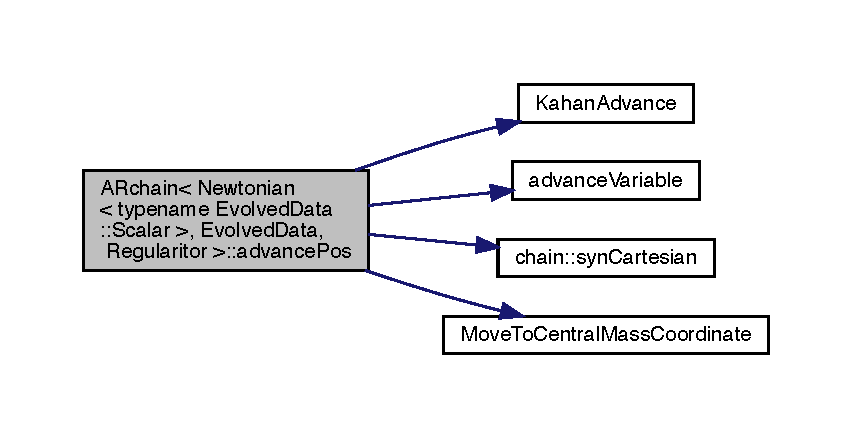
\includegraphics[width=350pt]{class_a_rchain_3_01_newtonian_3_01typename_01_evolved_data_1_1_scalar_01_4_00_01_evolved_data_00_01_regularitor_01_4_adffd5a74134d2a87e4f07908ea5beef4_cgraph}
\end{center}
\end{figure}
\mbox{\Hypertarget{class_a_rchain_3_01_newtonian_3_01typename_01_evolved_data_1_1_scalar_01_4_00_01_evolved_data_00_01_regularitor_01_4_ad11d21617228157e755aa334d9c621a7}\label{class_a_rchain_3_01_newtonian_3_01typename_01_evolved_data_1_1_scalar_01_4_00_01_evolved_data_00_01_regularitor_01_4_ad11d21617228157e755aa334d9c621a7}} 
\index{A\+Rchain$<$ Newtonian$<$ typename Evolved\+Data\+::\+Scalar $>$, Evolved\+Data, Regularitor $>$@{A\+Rchain$<$ Newtonian$<$ typename Evolved\+Data\+::\+Scalar $>$, Evolved\+Data, Regularitor $>$}!advance\+Vel@{advance\+Vel}}
\index{advance\+Vel@{advance\+Vel}!A\+Rchain$<$ Newtonian$<$ typename Evolved\+Data\+::\+Scalar $>$, Evolved\+Data, Regularitor $>$@{A\+Rchain$<$ Newtonian$<$ typename Evolved\+Data\+::\+Scalar $>$, Evolved\+Data, Regularitor $>$}}
\paragraph{\texorpdfstring{advance\+Vel()}{advanceVel()}}
{\footnotesize\ttfamily template$<$typename Evolved\+Data , typename Regularitor $>$ \\
void \mbox{\hyperlink{class_a_rchain}{A\+Rchain}}$<$ \mbox{\hyperlink{class_newtonian}{Newtonian}}$<$ typename \mbox{\hyperlink{class_a_rchain_a707e42a79e4744424a34c9007e84ee07}{Evolved\+Data\+::\+Scalar}} $>$, Evolved\+Data, Regularitor $>$\+::advance\+Vel (\begin{DoxyParamCaption}\item[{\mbox{\hyperlink{class_a_rchain_3_01_newtonian_3_01typename_01_evolved_data_1_1_scalar_01_4_00_01_evolved_data_00_01_regularitor_01_4_a2c77dc1b58a25ac5c6ee95dd7809f693}{Scalar}}}]{time\+Step\+Size }\end{DoxyParamCaption})}



Advance velocity one step with current acceleration. 

Advance chain velocity one step with current acceleration.

Advance chain velocity one step with current integration step size and accelerations. 
\begin{DoxyParams}{Parameters}
{\em time\+Step\+Size} & Integration step size, will be transfered to physical time in the function. \\
\hline
\end{DoxyParams}
Here is the call graph for this function\+:\nopagebreak
\begin{figure}[H]
\begin{center}
\leavevmode
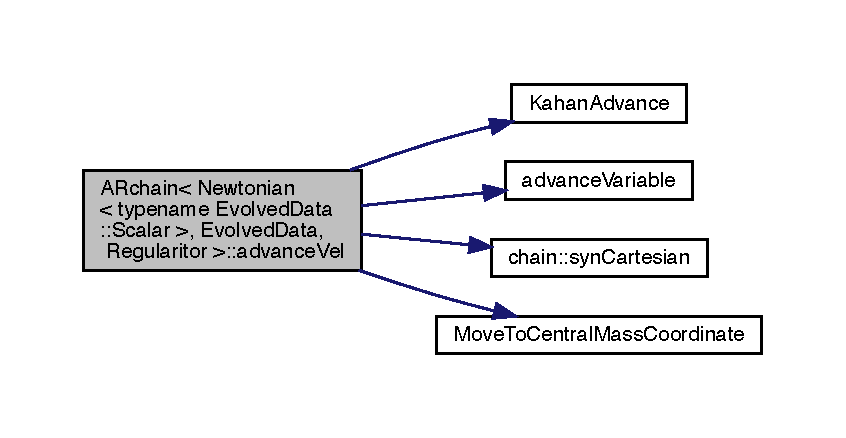
\includegraphics[width=350pt]{class_a_rchain_3_01_newtonian_3_01typename_01_evolved_data_1_1_scalar_01_4_00_01_evolved_data_00_01_regularitor_01_4_ad11d21617228157e755aa334d9c621a7_cgraph}
\end{center}
\end{figure}
\mbox{\Hypertarget{class_a_rchain_3_01_newtonian_3_01typename_01_evolved_data_1_1_scalar_01_4_00_01_evolved_data_00_01_regularitor_01_4_a919d200a913f75719c7240c030b9b113}\label{class_a_rchain_3_01_newtonian_3_01typename_01_evolved_data_1_1_scalar_01_4_00_01_evolved_data_00_01_regularitor_01_4_a919d200a913f75719c7240c030b9b113}} 
\index{A\+Rchain$<$ Newtonian$<$ typename Evolved\+Data\+::\+Scalar $>$, Evolved\+Data, Regularitor $>$@{A\+Rchain$<$ Newtonian$<$ typename Evolved\+Data\+::\+Scalar $>$, Evolved\+Data, Regularitor $>$}!array@{array}}
\index{array@{array}!A\+Rchain$<$ Newtonian$<$ typename Evolved\+Data\+::\+Scalar $>$, Evolved\+Data, Regularitor $>$@{A\+Rchain$<$ Newtonian$<$ typename Evolved\+Data\+::\+Scalar $>$, Evolved\+Data, Regularitor $>$}}
\paragraph{\texorpdfstring{array()}{array()}}
{\footnotesize\ttfamily template$<$typename Evolved\+Data , typename Regularitor $>$ \\
\mbox{\hyperlink{class_a_rchain_3_01_newtonian_3_01typename_01_evolved_data_1_1_scalar_01_4_00_01_evolved_data_00_01_regularitor_01_4_a8cf940df8dabb6c78662f839c2b13c9a}{Plain\+Array}}\& \mbox{\hyperlink{class_a_rchain}{A\+Rchain}}$<$ \mbox{\hyperlink{class_newtonian}{Newtonian}}$<$ typename \mbox{\hyperlink{class_a_rchain_a707e42a79e4744424a34c9007e84ee07}{Evolved\+Data\+::\+Scalar}} $>$, Evolved\+Data, Regularitor $>$\+::array (\begin{DoxyParamCaption}{ }\end{DoxyParamCaption})\hspace{0.3cm}{\ttfamily [inline]}}



Transfer the evolved data to a plain scalar array. 

\begin{DoxyNote}{Note}
Overload base class \mbox{\hyperlink{class_a_rchain_3_01_newtonian_3_01typename_01_evolved_data_1_1_scalar_01_4_00_01_evolved_data_00_01_regularitor_01_4_a919d200a913f75719c7240c030b9b113}{array()}}. 
\end{DoxyNote}
\mbox{\Hypertarget{class_a_rchain_3_01_newtonian_3_01typename_01_evolved_data_1_1_scalar_01_4_00_01_evolved_data_00_01_regularitor_01_4_a8e7bc5b32dbd7a0c9c3541f17fa54e28}\label{class_a_rchain_3_01_newtonian_3_01typename_01_evolved_data_1_1_scalar_01_4_00_01_evolved_data_00_01_regularitor_01_4_a8e7bc5b32dbd7a0c9c3541f17fa54e28}} 
\index{A\+Rchain$<$ Newtonian$<$ typename Evolved\+Data\+::\+Scalar $>$, Evolved\+Data, Regularitor $>$@{A\+Rchain$<$ Newtonian$<$ typename Evolved\+Data\+::\+Scalar $>$, Evolved\+Data, Regularitor $>$}!load@{load}}
\index{load@{load}!A\+Rchain$<$ Newtonian$<$ typename Evolved\+Data\+::\+Scalar $>$, Evolved\+Data, Regularitor $>$@{A\+Rchain$<$ Newtonian$<$ typename Evolved\+Data\+::\+Scalar $>$, Evolved\+Data, Regularitor $>$}}
\paragraph{\texorpdfstring{load()}{load()}}
{\footnotesize\ttfamily template$<$typename Evolved\+Data , typename Regularitor $>$ \\
void \mbox{\hyperlink{class_a_rchain}{A\+Rchain}}$<$ \mbox{\hyperlink{class_newtonian}{Newtonian}}$<$ typename \mbox{\hyperlink{class_a_rchain_a707e42a79e4744424a34c9007e84ee07}{Evolved\+Data\+::\+Scalar}} $>$, Evolved\+Data, Regularitor $>$\+::load (\begin{DoxyParamCaption}\item[{\mbox{\hyperlink{class_a_rchain_3_01_newtonian_3_01typename_01_evolved_data_1_1_scalar_01_4_00_01_evolved_data_00_01_regularitor_01_4_a8cf940df8dabb6c78662f839c2b13c9a}{Plain\+Array}} \&}]{data }\end{DoxyParamCaption})}



Load data from a plain array. 

\begin{DoxyNote}{Note}
Overload base class \mbox{\hyperlink{class_a_rchain_3_01_newtonian_3_01typename_01_evolved_data_1_1_scalar_01_4_00_01_evolved_data_00_01_regularitor_01_4_a8e7bc5b32dbd7a0c9c3541f17fa54e28}{load()}}.
\end{DoxyNote}
Interface usded by integrator and O\+DE iterator. Load data from a plain array processed by itegrator and iterator to chain data. Then synchrosize Cartesian data and update the chain. Derived class could overload this function to additional process.


\begin{DoxyParams}{Parameters}
{\em data} & Plain scalar array. \\
\hline
\end{DoxyParams}
Here is the call graph for this function\+:\nopagebreak
\begin{figure}[H]
\begin{center}
\leavevmode
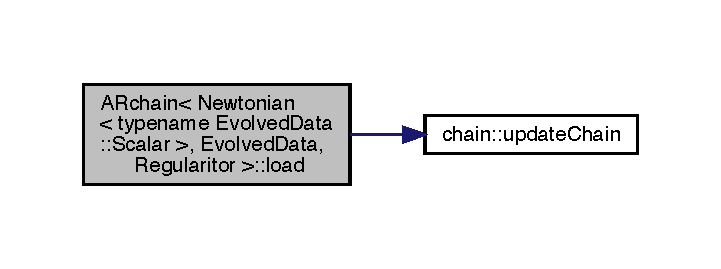
\includegraphics[width=346pt]{class_a_rchain_3_01_newtonian_3_01typename_01_evolved_data_1_1_scalar_01_4_00_01_evolved_data_00_01_regularitor_01_4_a8e7bc5b32dbd7a0c9c3541f17fa54e28_cgraph}
\end{center}
\end{figure}
\mbox{\Hypertarget{class_a_rchain_3_01_newtonian_3_01typename_01_evolved_data_1_1_scalar_01_4_00_01_evolved_data_00_01_regularitor_01_4_a577ecdf4e934627257a0824d59404831}\label{class_a_rchain_3_01_newtonian_3_01typename_01_evolved_data_1_1_scalar_01_4_00_01_evolved_data_00_01_regularitor_01_4_a577ecdf4e934627257a0824d59404831}} 
\index{A\+Rchain$<$ Newtonian$<$ typename Evolved\+Data\+::\+Scalar $>$, Evolved\+Data, Regularitor $>$@{A\+Rchain$<$ Newtonian$<$ typename Evolved\+Data\+::\+Scalar $>$, Evolved\+Data, Regularitor $>$}!operator=@{operator=}}
\index{operator=@{operator=}!A\+Rchain$<$ Newtonian$<$ typename Evolved\+Data\+::\+Scalar $>$, Evolved\+Data, Regularitor $>$@{A\+Rchain$<$ Newtonian$<$ typename Evolved\+Data\+::\+Scalar $>$, Evolved\+Data, Regularitor $>$}}
\paragraph{\texorpdfstring{operator=()}{operator=()}}
{\footnotesize\ttfamily template$<$typename Evolved\+Data , typename Regularitor $>$ \\
const \mbox{\hyperlink{class_a_rchain}{A\+Rchain}}$<$ \mbox{\hyperlink{class_newtonian}{Newtonian}}$<$ typename \mbox{\hyperlink{class_a_rchain_a707e42a79e4744424a34c9007e84ee07}{Evolved\+Data\+::\+Scalar}} $>$, Evolved\+Data, Regularitor $>$ \& \mbox{\hyperlink{class_a_rchain}{A\+Rchain}}$<$ \mbox{\hyperlink{class_newtonian}{Newtonian}}$<$ typename \mbox{\hyperlink{class_a_rchain_a707e42a79e4744424a34c9007e84ee07}{Evolved\+Data\+::\+Scalar}} $>$, Evolved\+Data, Regularitor $>$\+::operator= (\begin{DoxyParamCaption}\item[{const \mbox{\hyperlink{class_a_rchain}{A\+Rchain}}$<$ \mbox{\hyperlink{class_newtonian}{Newtonian}}$<$ typename \mbox{\hyperlink{class_a_rchain_a707e42a79e4744424a34c9007e84ee07}{Evolved\+Data\+::\+Scalar}} $>$, Evolved\+Data, Regularitor $>$ \&}]{other }\end{DoxyParamCaption})}



Overload operator =. 

\mbox{\Hypertarget{class_a_rchain_3_01_newtonian_3_01typename_01_evolved_data_1_1_scalar_01_4_00_01_evolved_data_00_01_regularitor_01_4_aa4b0a64e05c3942e402606e74c08b593}\label{class_a_rchain_3_01_newtonian_3_01typename_01_evolved_data_1_1_scalar_01_4_00_01_evolved_data_00_01_regularitor_01_4_aa4b0a64e05c3942e402606e74c08b593}} 
\index{A\+Rchain$<$ Newtonian$<$ typename Evolved\+Data\+::\+Scalar $>$, Evolved\+Data, Regularitor $>$@{A\+Rchain$<$ Newtonian$<$ typename Evolved\+Data\+::\+Scalar $>$, Evolved\+Data, Regularitor $>$}!read@{read}}
\index{read@{read}!A\+Rchain$<$ Newtonian$<$ typename Evolved\+Data\+::\+Scalar $>$, Evolved\+Data, Regularitor $>$@{A\+Rchain$<$ Newtonian$<$ typename Evolved\+Data\+::\+Scalar $>$, Evolved\+Data, Regularitor $>$}}
\paragraph{\texorpdfstring{read()}{read()}}
{\footnotesize\ttfamily template$<$typename Evolved\+Data , typename Regularitor $>$ \\
std\+::istream \& \mbox{\hyperlink{class_a_rchain}{A\+Rchain}}$<$ \mbox{\hyperlink{class_newtonian}{Newtonian}}$<$ typename \mbox{\hyperlink{class_a_rchain_a707e42a79e4744424a34c9007e84ee07}{Evolved\+Data\+::\+Scalar}} $>$, Evolved\+Data, Regularitor $>$\+::read (\begin{DoxyParamCaption}\item[{std\+::istream \&}]{input }\end{DoxyParamCaption})}



Input data from standard c++ istream. 

\begin{DoxyNote}{Note}
Overload base class \mbox{\hyperlink{class_a_rchain_3_01_newtonian_3_01typename_01_evolved_data_1_1_scalar_01_4_00_01_evolved_data_00_01_regularitor_01_4_aa4b0a64e05c3942e402606e74c08b593}{read()}}.
\end{DoxyNote}
Implement of C\+R\+TP \textquotesingle{}$>$$>$\textquotesingle{} method. Here is the call graph for this function\+:\nopagebreak
\begin{figure}[H]
\begin{center}
\leavevmode
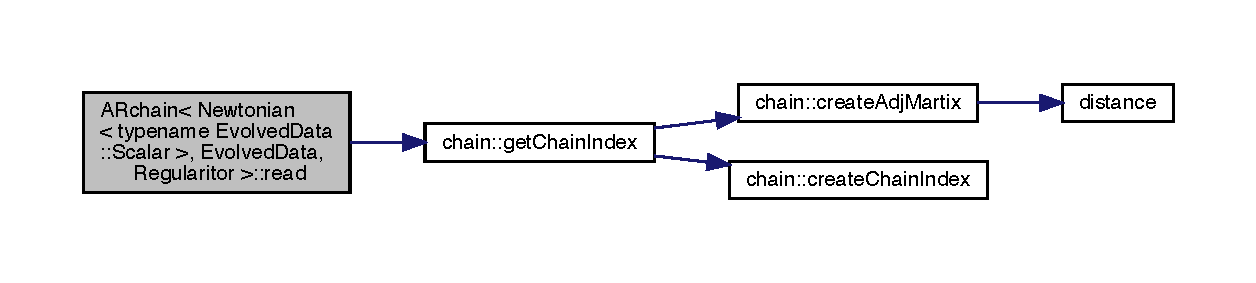
\includegraphics[width=350pt]{class_a_rchain_3_01_newtonian_3_01typename_01_evolved_data_1_1_scalar_01_4_00_01_evolved_data_00_01_regularitor_01_4_aa4b0a64e05c3942e402606e74c08b593_cgraph}
\end{center}
\end{figure}
\mbox{\Hypertarget{class_a_rchain_3_01_newtonian_3_01typename_01_evolved_data_1_1_scalar_01_4_00_01_evolved_data_00_01_regularitor_01_4_a928601b10d9a9e5ab02f36cf11efa263}\label{class_a_rchain_3_01_newtonian_3_01typename_01_evolved_data_1_1_scalar_01_4_00_01_evolved_data_00_01_regularitor_01_4_a928601b10d9a9e5ab02f36cf11efa263}} 
\index{A\+Rchain$<$ Newtonian$<$ typename Evolved\+Data\+::\+Scalar $>$, Evolved\+Data, Regularitor $>$@{A\+Rchain$<$ Newtonian$<$ typename Evolved\+Data\+::\+Scalar $>$, Evolved\+Data, Regularitor $>$}!size@{size}}
\index{size@{size}!A\+Rchain$<$ Newtonian$<$ typename Evolved\+Data\+::\+Scalar $>$, Evolved\+Data, Regularitor $>$@{A\+Rchain$<$ Newtonian$<$ typename Evolved\+Data\+::\+Scalar $>$, Evolved\+Data, Regularitor $>$}}
\paragraph{\texorpdfstring{size()}{size()}}
{\footnotesize\ttfamily template$<$typename Evolved\+Data , typename Regularitor $>$ \\
static constexpr size\+\_\+t \mbox{\hyperlink{class_a_rchain}{A\+Rchain}}$<$ \mbox{\hyperlink{class_newtonian}{Newtonian}}$<$ typename \mbox{\hyperlink{class_a_rchain_a707e42a79e4744424a34c9007e84ee07}{Evolved\+Data\+::\+Scalar}} $>$, Evolved\+Data, Regularitor $>$\+::size (\begin{DoxyParamCaption}{ }\end{DoxyParamCaption})\hspace{0.3cm}{\ttfamily [inline]}, {\ttfamily [static]}}



Get the number of the particles. 

\begin{DoxyReturn}{Returns}
The particle number. 
\end{DoxyReturn}
\begin{DoxyNote}{Note}
Overload base class \mbox{\hyperlink{class_a_rchain_3_01_newtonian_3_01typename_01_evolved_data_1_1_scalar_01_4_00_01_evolved_data_00_01_regularitor_01_4_a928601b10d9a9e5ab02f36cf11efa263}{size()}}. 
\end{DoxyNote}
\mbox{\Hypertarget{class_a_rchain_3_01_newtonian_3_01typename_01_evolved_data_1_1_scalar_01_4_00_01_evolved_data_00_01_regularitor_01_4_aa7aadb0b5ffcfebc759e4f091c4fc763}\label{class_a_rchain_3_01_newtonian_3_01typename_01_evolved_data_1_1_scalar_01_4_00_01_evolved_data_00_01_regularitor_01_4_aa7aadb0b5ffcfebc759e4f091c4fc763}} 
\index{A\+Rchain$<$ Newtonian$<$ typename Evolved\+Data\+::\+Scalar $>$, Evolved\+Data, Regularitor $>$@{A\+Rchain$<$ Newtonian$<$ typename Evolved\+Data\+::\+Scalar $>$, Evolved\+Data, Regularitor $>$}!time\+Scale@{time\+Scale}}
\index{time\+Scale@{time\+Scale}!A\+Rchain$<$ Newtonian$<$ typename Evolved\+Data\+::\+Scalar $>$, Evolved\+Data, Regularitor $>$@{A\+Rchain$<$ Newtonian$<$ typename Evolved\+Data\+::\+Scalar $>$, Evolved\+Data, Regularitor $>$}}
\paragraph{\texorpdfstring{time\+Scale()}{timeScale()}}
{\footnotesize\ttfamily template$<$typename Evolved\+Data , typename Regularitor $>$ \\
\mbox{\hyperlink{class_a_rchain_a707e42a79e4744424a34c9007e84ee07}{Evolved\+Data\+::\+Scalar}} \mbox{\hyperlink{class_a_rchain}{A\+Rchain}}$<$ \mbox{\hyperlink{class_newtonian}{Newtonian}}$<$ typename \mbox{\hyperlink{class_a_rchain_a707e42a79e4744424a34c9007e84ee07}{Evolved\+Data\+::\+Scalar}} $>$, Evolved\+Data, Regularitor $>$\+::time\+Scale (\begin{DoxyParamCaption}\item[{\mbox{\hyperlink{class_a_rchain_3_01_newtonian_3_01typename_01_evolved_data_1_1_scalar_01_4_00_01_evolved_data_00_01_regularitor_01_4_a2c77dc1b58a25ac5c6ee95dd7809f693}{Scalar}}}]{scale }\end{DoxyParamCaption})}



Interface to rescale the time. 

\begin{DoxyNote}{Note}
Overload base class \mbox{\hyperlink{class_a_rchain_3_01_newtonian_3_01typename_01_evolved_data_1_1_scalar_01_4_00_01_evolved_data_00_01_regularitor_01_4_aa7aadb0b5ffcfebc759e4f091c4fc763}{time\+Scale()}}.
\end{DoxyNote}
Interace used by dynamic system. Transfer integration time to physical time. \begin{DoxyReturn}{Returns}
The phsyical time. 
\end{DoxyReturn}
\mbox{\Hypertarget{class_a_rchain_3_01_newtonian_3_01typename_01_evolved_data_1_1_scalar_01_4_00_01_evolved_data_00_01_regularitor_01_4_acbe31e9aa918e4f80a2763e16f0bb7bc}\label{class_a_rchain_3_01_newtonian_3_01typename_01_evolved_data_1_1_scalar_01_4_00_01_evolved_data_00_01_regularitor_01_4_acbe31e9aa918e4f80a2763e16f0bb7bc}} 
\index{A\+Rchain$<$ Newtonian$<$ typename Evolved\+Data\+::\+Scalar $>$, Evolved\+Data, Regularitor $>$@{A\+Rchain$<$ Newtonian$<$ typename Evolved\+Data\+::\+Scalar $>$, Evolved\+Data, Regularitor $>$}!update\+Chain@{update\+Chain}}
\index{update\+Chain@{update\+Chain}!A\+Rchain$<$ Newtonian$<$ typename Evolved\+Data\+::\+Scalar $>$, Evolved\+Data, Regularitor $>$@{A\+Rchain$<$ Newtonian$<$ typename Evolved\+Data\+::\+Scalar $>$, Evolved\+Data, Regularitor $>$}}
\paragraph{\texorpdfstring{update\+Chain()}{updateChain()}}
{\footnotesize\ttfamily template$<$typename Evolved\+Data , typename Regularitor $>$ \\
void \mbox{\hyperlink{class_a_rchain}{A\+Rchain}}$<$ \mbox{\hyperlink{class_newtonian}{Newtonian}}$<$ typename \mbox{\hyperlink{class_a_rchain_a707e42a79e4744424a34c9007e84ee07}{Evolved\+Data\+::\+Scalar}} $>$, Evolved\+Data, Regularitor $>$\+::update\+Chain (\begin{DoxyParamCaption}{ }\end{DoxyParamCaption})\hspace{0.3cm}{\ttfamily [private]}}



Update the chain data based on current Cartesian coordinates. 

Update chain index and chain.

Due to the evolution, the relative position of particles may vary with time. This function update the chain index and chain if needed. Here is the call graph for this function\+:\nopagebreak
\begin{figure}[H]
\begin{center}
\leavevmode
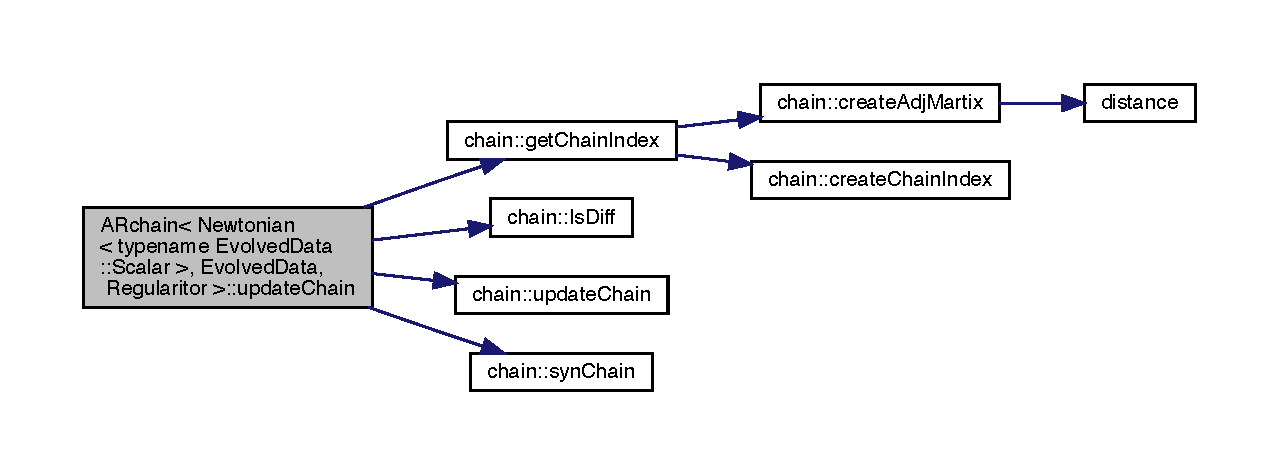
\includegraphics[width=350pt]{class_a_rchain_3_01_newtonian_3_01typename_01_evolved_data_1_1_scalar_01_4_00_01_evolved_data_00_01_regularitor_01_4_acbe31e9aa918e4f80a2763e16f0bb7bc_cgraph}
\end{center}
\end{figure}
\mbox{\Hypertarget{class_a_rchain_3_01_newtonian_3_01typename_01_evolved_data_1_1_scalar_01_4_00_01_evolved_data_00_01_regularitor_01_4_a2b11ca856564416ed6727c716ed284a8}\label{class_a_rchain_3_01_newtonian_3_01typename_01_evolved_data_1_1_scalar_01_4_00_01_evolved_data_00_01_regularitor_01_4_a2b11ca856564416ed6727c716ed284a8}} 
\index{A\+Rchain$<$ Newtonian$<$ typename Evolved\+Data\+::\+Scalar $>$, Evolved\+Data, Regularitor $>$@{A\+Rchain$<$ Newtonian$<$ typename Evolved\+Data\+::\+Scalar $>$, Evolved\+Data, Regularitor $>$}!update\+Vel\+Indep\+Acc@{update\+Vel\+Indep\+Acc}}
\index{update\+Vel\+Indep\+Acc@{update\+Vel\+Indep\+Acc}!A\+Rchain$<$ Newtonian$<$ typename Evolved\+Data\+::\+Scalar $>$, Evolved\+Data, Regularitor $>$@{A\+Rchain$<$ Newtonian$<$ typename Evolved\+Data\+::\+Scalar $>$, Evolved\+Data, Regularitor $>$}}
\paragraph{\texorpdfstring{update\+Vel\+Indep\+Acc()}{updateVelIndepAcc()}}
{\footnotesize\ttfamily template$<$typename Evolved\+Data , typename Regularitor $>$ \\
void \mbox{\hyperlink{class_a_rchain}{A\+Rchain}}$<$ \mbox{\hyperlink{class_newtonian}{Newtonian}}$<$ typename \mbox{\hyperlink{class_a_rchain_a707e42a79e4744424a34c9007e84ee07}{Evolved\+Data\+::\+Scalar}} $>$, Evolved\+Data, Regularitor $>$\+::update\+Vel\+Indep\+Acc (\begin{DoxyParamCaption}{ }\end{DoxyParamCaption})\hspace{0.3cm}{\ttfamily [private]}}



Update velocity independent acceleration. 

Update velocity independent acceleration \textquotesingle{}vel\+Indep\+Acc\textquotesingle{} based on \mbox{\hyperlink{class_newtonian}{Newtonian}} interaction with chain data. Then calculate the corresponding chain acceleration. 

\subsubsection{Member Data Documentation}
\mbox{\Hypertarget{class_a_rchain_3_01_newtonian_3_01typename_01_evolved_data_1_1_scalar_01_4_00_01_evolved_data_00_01_regularitor_01_4_a39576accb53257bdb1b55e6d21acdf0f}\label{class_a_rchain_3_01_newtonian_3_01typename_01_evolved_data_1_1_scalar_01_4_00_01_evolved_data_00_01_regularitor_01_4_a39576accb53257bdb1b55e6d21acdf0f}} 
\index{A\+Rchain$<$ Newtonian$<$ typename Evolved\+Data\+::\+Scalar $>$, Evolved\+Data, Regularitor $>$@{A\+Rchain$<$ Newtonian$<$ typename Evolved\+Data\+::\+Scalar $>$, Evolved\+Data, Regularitor $>$}!chain@{chain}}
\index{chain@{chain}!A\+Rchain$<$ Newtonian$<$ typename Evolved\+Data\+::\+Scalar $>$, Evolved\+Data, Regularitor $>$@{A\+Rchain$<$ Newtonian$<$ typename Evolved\+Data\+::\+Scalar $>$, Evolved\+Data, Regularitor $>$}}
\paragraph{\texorpdfstring{chain}{chain}}
{\footnotesize\ttfamily template$<$typename Evolved\+Data , typename Regularitor $>$ \\
Evolved\+Data \mbox{\hyperlink{class_a_rchain}{A\+Rchain}}$<$ \mbox{\hyperlink{class_newtonian}{Newtonian}}$<$ typename \mbox{\hyperlink{class_a_rchain_a707e42a79e4744424a34c9007e84ee07}{Evolved\+Data\+::\+Scalar}} $>$, Evolved\+Data, Regularitor $>$\+::chain\hspace{0.3cm}{\ttfamily [private]}}



Evolved variables in chain coordinates. 

\mbox{\Hypertarget{class_a_rchain_3_01_newtonian_3_01typename_01_evolved_data_1_1_scalar_01_4_00_01_evolved_data_00_01_regularitor_01_4_a6a8ef156105e2f80dc143606d4ba10c9}\label{class_a_rchain_3_01_newtonian_3_01typename_01_evolved_data_1_1_scalar_01_4_00_01_evolved_data_00_01_regularitor_01_4_a6a8ef156105e2f80dc143606d4ba10c9}} 
\index{A\+Rchain$<$ Newtonian$<$ typename Evolved\+Data\+::\+Scalar $>$, Evolved\+Data, Regularitor $>$@{A\+Rchain$<$ Newtonian$<$ typename Evolved\+Data\+::\+Scalar $>$, Evolved\+Data, Regularitor $>$}!chain\+Index@{chain\+Index}}
\index{chain\+Index@{chain\+Index}!A\+Rchain$<$ Newtonian$<$ typename Evolved\+Data\+::\+Scalar $>$, Evolved\+Data, Regularitor $>$@{A\+Rchain$<$ Newtonian$<$ typename Evolved\+Data\+::\+Scalar $>$, Evolved\+Data, Regularitor $>$}}
\paragraph{\texorpdfstring{chain\+Index}{chainIndex}}
{\footnotesize\ttfamily template$<$typename Evolved\+Data , typename Regularitor $>$ \\
\mbox{\hyperlink{class_a_rchain_3_01_newtonian_3_01typename_01_evolved_data_1_1_scalar_01_4_00_01_evolved_data_00_01_regularitor_01_4_a0072f8585c3e6ba8d64cb81be90fb376}{Index\+Array}} \mbox{\hyperlink{class_a_rchain}{A\+Rchain}}$<$ \mbox{\hyperlink{class_newtonian}{Newtonian}}$<$ typename \mbox{\hyperlink{class_a_rchain_a707e42a79e4744424a34c9007e84ee07}{Evolved\+Data\+::\+Scalar}} $>$, Evolved\+Data, Regularitor $>$\+::chain\+Index\hspace{0.3cm}{\ttfamily [private]}}



Mapping index from Cartesian coordinates to chain coordinates. 

\mbox{\Hypertarget{class_a_rchain_3_01_newtonian_3_01typename_01_evolved_data_1_1_scalar_01_4_00_01_evolved_data_00_01_regularitor_01_4_a6e5a31aa07620ab9f3503ebc412ff969}\label{class_a_rchain_3_01_newtonian_3_01typename_01_evolved_data_1_1_scalar_01_4_00_01_evolved_data_00_01_regularitor_01_4_a6e5a31aa07620ab9f3503ebc412ff969}} 
\index{A\+Rchain$<$ Newtonian$<$ typename Evolved\+Data\+::\+Scalar $>$, Evolved\+Data, Regularitor $>$@{A\+Rchain$<$ Newtonian$<$ typename Evolved\+Data\+::\+Scalar $>$, Evolved\+Data, Regularitor $>$}!regular@{regular}}
\index{regular@{regular}!A\+Rchain$<$ Newtonian$<$ typename Evolved\+Data\+::\+Scalar $>$, Evolved\+Data, Regularitor $>$@{A\+Rchain$<$ Newtonian$<$ typename Evolved\+Data\+::\+Scalar $>$, Evolved\+Data, Regularitor $>$}}
\paragraph{\texorpdfstring{regular}{regular}}
{\footnotesize\ttfamily template$<$typename Evolved\+Data , typename Regularitor $>$ \\
Regularitor \mbox{\hyperlink{class_a_rchain}{A\+Rchain}}$<$ \mbox{\hyperlink{class_newtonian}{Newtonian}}$<$ typename \mbox{\hyperlink{class_a_rchain_a707e42a79e4744424a34c9007e84ee07}{Evolved\+Data\+::\+Scalar}} $>$, Evolved\+Data, Regularitor $>$\+::regular\hspace{0.3cm}{\ttfamily [private]}}



Regularization interface. 

\mbox{\Hypertarget{class_a_rchain_3_01_newtonian_3_01typename_01_evolved_data_1_1_scalar_01_4_00_01_evolved_data_00_01_regularitor_01_4_af0862cdda12b7ba2ba5d5d098d008398}\label{class_a_rchain_3_01_newtonian_3_01typename_01_evolved_data_1_1_scalar_01_4_00_01_evolved_data_00_01_regularitor_01_4_af0862cdda12b7ba2ba5d5d098d008398}} 
\index{A\+Rchain$<$ Newtonian$<$ typename Evolved\+Data\+::\+Scalar $>$, Evolved\+Data, Regularitor $>$@{A\+Rchain$<$ Newtonian$<$ typename Evolved\+Data\+::\+Scalar $>$, Evolved\+Data, Regularitor $>$}!vel\+Indep\+Acc@{vel\+Indep\+Acc}}
\index{vel\+Indep\+Acc@{vel\+Indep\+Acc}!A\+Rchain$<$ Newtonian$<$ typename Evolved\+Data\+::\+Scalar $>$, Evolved\+Data, Regularitor $>$@{A\+Rchain$<$ Newtonian$<$ typename Evolved\+Data\+::\+Scalar $>$, Evolved\+Data, Regularitor $>$}}
\paragraph{\texorpdfstring{vel\+Indep\+Acc}{velIndepAcc}}
{\footnotesize\ttfamily template$<$typename Evolved\+Data , typename Regularitor $>$ \\
\mbox{\hyperlink{class_a_rchain_3_01_newtonian_3_01typename_01_evolved_data_1_1_scalar_01_4_00_01_evolved_data_00_01_regularitor_01_4_a1ff7d2e64f488df9edae2ad796945bbd}{Vector\+Array}} \mbox{\hyperlink{class_a_rchain}{A\+Rchain}}$<$ \mbox{\hyperlink{class_newtonian}{Newtonian}}$<$ typename \mbox{\hyperlink{class_a_rchain_a707e42a79e4744424a34c9007e84ee07}{Evolved\+Data\+::\+Scalar}} $>$, Evolved\+Data, Regularitor $>$\+::vel\+Indep\+Acc\hspace{0.3cm}{\ttfamily [private]}}



Velocity independent acceleration array in Cartesian coordiantes. 



The documentation for this class was generated from the following file\+:\begin{DoxyCompactItemize}
\item 
particle\+System/\mbox{\hyperlink{_a_rchain_8h}{A\+Rchain.\+h}}\end{DoxyCompactItemize}

\hypertarget{class_b_s_iterator}{}\subsection{B\+S\+Iterator$<$ Partic\+Sys, Integrator $>$ Class Template Reference}
\label{class_b_s_iterator}\index{B\+S\+Iterator$<$ Partic\+Sys, Integrator $>$@{B\+S\+Iterator$<$ Partic\+Sys, Integrator $>$}}


Bulirsch-\/\+Stoer extrapolation algorithm.  




{\ttfamily \#include $<$B\+S\+Iterator.\+h$>$}

\subsubsection*{Public Types}
\begin{DoxyCompactItemize}
\item 
typedef Partic\+Sys\+::\+Scalar \mbox{\hyperlink{class_b_s_iterator_a7857f8ff9032955ea4dcc22cd18ca7a1}{Scalar}}
\item 
{\footnotesize template$<$typename Scalar , size\+\_\+t N$>$ }\\using \mbox{\hyperlink{class_b_s_iterator_ab0aa7c10b56500273af05dcd85fd8389}{scalar\+Array}} = std\+::array$<$ \mbox{\hyperlink{class_b_s_iterator_a7857f8ff9032955ea4dcc22cd18ca7a1}{Scalar}}, N $>$
\end{DoxyCompactItemize}
\subsubsection*{Public Member Functions}
\begin{DoxyCompactItemize}
\item 
\mbox{\hyperlink{class_b_s_iterator_a144fb5c55fcd7bc873e73f4d06276fb2}{B\+S\+Iterator}} ()
\begin{DoxyCompactList}\small\item\em Constructor for initializing cost, n\+Steps, fmin and CC. \end{DoxyCompactList}\item 
\mbox{\hyperlink{class_b_s_iterator_a7857f8ff9032955ea4dcc22cd18ca7a1}{Scalar}} \mbox{\hyperlink{class_b_s_iterator_a5520642ecbd454fb1f4d9ece18dc4e3f}{iterate}} (Partic\+Sys \&particles, Integrator \&integrator, \mbox{\hyperlink{class_b_s_iterator_a7857f8ff9032955ea4dcc22cd18ca7a1}{Scalar}} step\+Length)
\begin{DoxyCompactList}\small\item\em Interface of O\+DE iterator. \end{DoxyCompactList}\item 
void \mbox{\hyperlink{class_b_s_iterator_ada9b6cc673e297135646699d581fcdc7}{set\+Relative\+Error}} (\mbox{\hyperlink{class_b_s_iterator_a7857f8ff9032955ea4dcc22cd18ca7a1}{Scalar}} rel\+Error)
\begin{DoxyCompactList}\small\item\em Set the local relative error. \end{DoxyCompactList}\item 
void \mbox{\hyperlink{class_b_s_iterator_a57603539823be271c2229d0951b7d957}{set\+Absolute\+Error}} (\mbox{\hyperlink{class_b_s_iterator_a7857f8ff9032955ea4dcc22cd18ca7a1}{Scalar}} abs\+Error)
\begin{DoxyCompactList}\small\item\em Set the local absolute error. \end{DoxyCompactList}\end{DoxyCompactItemize}
\subsubsection*{Private Member Functions}
\begin{DoxyCompactItemize}
\item 
void \mbox{\hyperlink{class_b_s_iterator_a95c268219a8321af35a628db4e22bec4}{copy\+Data\+To\+Extrap\+Tab}} (size\+\_\+t k)
\begin{DoxyCompactList}\small\item\em Copy the current results of localsystem as a plain array to the first column of extrapolation talbe. \end{DoxyCompactList}\item 
bool \mbox{\hyperlink{class_b_s_iterator_a42976d786ffe422a86cc5a7b0a077609}{check\+Rejection}} (\mbox{\hyperlink{class_b_s_iterator_a7857f8ff9032955ea4dcc22cd18ca7a1}{Scalar}} error, size\+\_\+t k) const
\begin{DoxyCompactList}\small\item\em Check the rejection criteria for current iteration. \end{DoxyCompactList}\item 
void \mbox{\hyperlink{class_b_s_iterator_ac1edf158e3dd05ed15afd5d0f31c121a}{extrapolate}} (size\+\_\+t k)
\begin{DoxyCompactList}\small\item\em Extrapolate the kth row to the right end. \end{DoxyCompactList}\item 
\mbox{\hyperlink{class_b_s_iterator_a7857f8ff9032955ea4dcc22cd18ca7a1}{Scalar}} \mbox{\hyperlink{class_b_s_iterator_a9f50e084f8650e4d7fea3535a0547139}{get\+Error}} (size\+\_\+t k) const
\begin{DoxyCompactList}\small\item\em Calculate the error of the k row of the extrapolation table. \end{DoxyCompactList}\item 
\mbox{\hyperlink{class_b_s_iterator_a7857f8ff9032955ea4dcc22cd18ca7a1}{Scalar}} \mbox{\hyperlink{class_b_s_iterator_a9d06a0d0c9e458ea96952b0514adece9}{get\+Time\+Step\+Coef}} (\mbox{\hyperlink{class_b_s_iterator_a7857f8ff9032955ea4dcc22cd18ca7a1}{Scalar}} error, size\+\_\+t order)
\begin{DoxyCompactList}\small\item\em Calculate the new iteration integration step coefficient. \end{DoxyCompactList}\item 
\mbox{\hyperlink{class_b_s_iterator_a7857f8ff9032955ea4dcc22cd18ca7a1}{Scalar}} \mbox{\hyperlink{class_b_s_iterator_a738a558ddfacd9959c9438862001d7e8}{prepare\+For\+New\+Iteration}} (size\+\_\+t k, bool last\+Rejection)
\begin{DoxyCompactList}\small\item\em Calculate the new iteration integration step and new iteration depth for next iteration. \end{DoxyCompactList}\end{DoxyCompactItemize}
\subsubsection*{Private Attributes}
\begin{DoxyCompactItemize}
\item 
Partic\+Sys \mbox{\hyperlink{class_b_s_iterator_a9d6fc5f237246465161ea86854985395}{local\+System}}
\begin{DoxyCompactList}\small\item\em The local partical system used to iterate. \end{DoxyCompactList}\item 
\mbox{\hyperlink{class_b_s_iterator_ab0aa7c10b56500273af05dcd85fd8389}{scalar\+Array}}$<$ \mbox{\hyperlink{class_b_s_iterator_ab0aa7c10b56500273af05dcd85fd8389}{scalar\+Array}}$<$ \mbox{\hyperlink{class_b_s_iterator_a7857f8ff9032955ea4dcc22cd18ca7a1}{Scalar}}, Partic\+Sys\+::volume()$>$,(\mbox{\hyperlink{class_b_s_iterator_a39409b9a12d4854d101ce59a0efc0f74}{Max\+Depth}}+1) $\ast$(\mbox{\hyperlink{class_b_s_iterator_a39409b9a12d4854d101ce59a0efc0f74}{Max\+Depth}}+2)/2 $>$ \mbox{\hyperlink{class_b_s_iterator_aa501e973f342248fc445d59a5166ccc9}{extrap\+Tab}}
\begin{DoxyCompactList}\small\item\em Extrapolation table. \end{DoxyCompactList}\item 
\mbox{\hyperlink{class_b_s_iterator_ab0aa7c10b56500273af05dcd85fd8389}{scalar\+Array}}$<$ \mbox{\hyperlink{class_b_s_iterator_a7857f8ff9032955ea4dcc22cd18ca7a1}{Scalar}},(\mbox{\hyperlink{class_b_s_iterator_a39409b9a12d4854d101ce59a0efc0f74}{Max\+Depth}}+1) $\ast$(\mbox{\hyperlink{class_b_s_iterator_a39409b9a12d4854d101ce59a0efc0f74}{Max\+Depth}}+2)/2 $>$ \mbox{\hyperlink{class_b_s_iterator_a28f6cc2fd6bfd554f85225492f4210b7}{CC}}
\begin{DoxyCompactList}\small\item\em Extrapolation coefficient. \end{DoxyCompactList}\item 
\mbox{\hyperlink{class_b_s_iterator_ab0aa7c10b56500273af05dcd85fd8389}{scalar\+Array}}$<$ \mbox{\hyperlink{class_b_s_iterator_a7857f8ff9032955ea4dcc22cd18ca7a1}{Scalar}}, \mbox{\hyperlink{class_b_s_iterator_a39409b9a12d4854d101ce59a0efc0f74}{Max\+Depth}}+1 $>$ \mbox{\hyperlink{class_b_s_iterator_a96c58777cbefe7d02e160317621fc0b9}{macro\+Step\+Length}}
\begin{DoxyCompactList}\small\item\em Macro step length for different iteration depth. \end{DoxyCompactList}\item 
\mbox{\hyperlink{class_b_s_iterator_ab0aa7c10b56500273af05dcd85fd8389}{scalar\+Array}}$<$ \mbox{\hyperlink{class_b_s_iterator_a7857f8ff9032955ea4dcc22cd18ca7a1}{Scalar}}, \mbox{\hyperlink{class_b_s_iterator_a39409b9a12d4854d101ce59a0efc0f74}{Max\+Depth}}+1 $>$ \mbox{\hyperlink{class_b_s_iterator_ac2a338d6c3e5014d529666032d34c987}{work}}
\begin{DoxyCompactList}\small\item\em The work(calculation quantities) per integration length of each iteration depth. \end{DoxyCompactList}\item 
\mbox{\hyperlink{class_b_s_iterator_ab0aa7c10b56500273af05dcd85fd8389}{scalar\+Array}}$<$ \mbox{\hyperlink{class_b_s_iterator_a7857f8ff9032955ea4dcc22cd18ca7a1}{Scalar}}, \mbox{\hyperlink{class_b_s_iterator_a39409b9a12d4854d101ce59a0efc0f74}{Max\+Depth}}+1 $>$ \mbox{\hyperlink{class_b_s_iterator_a05bf5c727d23e47349683cda1a08ed13}{fmin}}
\begin{DoxyCompactList}\small\item\em The minimal coeffient of integration step estimation. \end{DoxyCompactList}\item 
\mbox{\hyperlink{class_b_s_iterator_ab0aa7c10b56500273af05dcd85fd8389}{scalar\+Array}}$<$ size\+\_\+t, \mbox{\hyperlink{class_b_s_iterator_a39409b9a12d4854d101ce59a0efc0f74}{Max\+Depth}}+1 $>$ \mbox{\hyperlink{class_b_s_iterator_a53f435811c23c0ae1713df13197fc9c9}{cost}}
\begin{DoxyCompactList}\small\item\em The work(calculation quantities) of each iteration depth. \end{DoxyCompactList}\item 
\mbox{\hyperlink{class_b_s_iterator_ab0aa7c10b56500273af05dcd85fd8389}{scalar\+Array}}$<$ size\+\_\+t, \mbox{\hyperlink{class_b_s_iterator_a39409b9a12d4854d101ce59a0efc0f74}{Max\+Depth}}+1 $>$ \mbox{\hyperlink{class_b_s_iterator_a9c4c8c17a759cdff694e0bd62ed249bd}{n\+Steps}}
\begin{DoxyCompactList}\small\item\em Steps of integration of each iteration depth. \end{DoxyCompactList}\item 
\mbox{\hyperlink{class_b_s_iterator_a7857f8ff9032955ea4dcc22cd18ca7a1}{Scalar}} \mbox{\hyperlink{class_b_s_iterator_a8948aa04b0ec390d43eb3d1f0a2efb03}{absolute\+Error}} \{1e-\/15\}
\begin{DoxyCompactList}\small\item\em Local absolute error. \end{DoxyCompactList}\item 
\mbox{\hyperlink{class_b_s_iterator_a7857f8ff9032955ea4dcc22cd18ca7a1}{Scalar}} \mbox{\hyperlink{class_b_s_iterator_abce71b7bac10363f7772dc848f8722b6}{relative\+Error}} \{1e-\/15\}
\begin{DoxyCompactList}\small\item\em Local relative error. \end{DoxyCompactList}\item 
\mbox{\hyperlink{class_b_s_iterator_a7857f8ff9032955ea4dcc22cd18ca7a1}{Scalar}} \mbox{\hyperlink{class_b_s_iterator_a942f85e00c28ef1990d1dfbed69c9e13}{s1}} \{0.\+94\}
\begin{DoxyCompactList}\small\item\em Coefficient of new step length estimation. See \char`\"{}\+Numerical recipes\char`\"{} on page 926. \end{DoxyCompactList}\item 
\mbox{\hyperlink{class_b_s_iterator_a7857f8ff9032955ea4dcc22cd18ca7a1}{Scalar}} \mbox{\hyperlink{class_b_s_iterator_ad1cdde25df6bca7a456c1908be54065f}{s2}} \{0.\+95\}
\begin{DoxyCompactList}\small\item\em Coefficient of new step length estimation. \end{DoxyCompactList}\item 
\mbox{\hyperlink{class_b_s_iterator_a7857f8ff9032955ea4dcc22cd18ca7a1}{Scalar}} \mbox{\hyperlink{class_b_s_iterator_a10ea0bb96f7971e9c477daef1fda6e16}{s3}} \{0.\+02\}
\begin{DoxyCompactList}\small\item\em Coefficient of new step length estimation. \end{DoxyCompactList}\item 
\mbox{\hyperlink{class_b_s_iterator_a7857f8ff9032955ea4dcc22cd18ca7a1}{Scalar}} \mbox{\hyperlink{class_b_s_iterator_a5b3bbb2d988a5d91030060508e3b4f66}{s4}} \{4.\+0\}
\begin{DoxyCompactList}\small\item\em Coefficient of new step length estimation. \end{DoxyCompactList}\item 
size\+\_\+t \mbox{\hyperlink{class_b_s_iterator_aa073f847cc5855f727c8f326f539a5f0}{iter\+Depth}} \{7\}
\begin{DoxyCompactList}\small\item\em Current iteraation depth. \end{DoxyCompactList}\end{DoxyCompactItemize}
\subsubsection*{Static Private Attributes}
\begin{DoxyCompactItemize}
\item 
static const size\+\_\+t \mbox{\hyperlink{class_b_s_iterator_a39409b9a12d4854d101ce59a0efc0f74}{Max\+Depth}} \{8\}
\begin{DoxyCompactList}\small\item\em The Maximum iteration depth. \end{DoxyCompactList}\end{DoxyCompactItemize}


\subsubsection{Detailed Description}
\subsubsection*{template$<$typename Partic\+Sys, typename Integrator$>$\newline
class B\+S\+Iterator$<$ Partic\+Sys, Integrator $>$}

Bulirsch-\/\+Stoer extrapolation algorithm. 

\subsubsection{Member Typedef Documentation}
\mbox{\Hypertarget{class_b_s_iterator_a7857f8ff9032955ea4dcc22cd18ca7a1}\label{class_b_s_iterator_a7857f8ff9032955ea4dcc22cd18ca7a1}} 
\index{B\+S\+Iterator@{B\+S\+Iterator}!Scalar@{Scalar}}
\index{Scalar@{Scalar}!B\+S\+Iterator@{B\+S\+Iterator}}
\paragraph{\texorpdfstring{Scalar}{Scalar}}
{\footnotesize\ttfamily template$<$typename Partic\+Sys , typename Integrator $>$ \\
typedef Partic\+Sys\+::\+Scalar \mbox{\hyperlink{class_b_s_iterator}{B\+S\+Iterator}}$<$ Partic\+Sys, Integrator $>$\+::\mbox{\hyperlink{class_b_s_iterator_a7857f8ff9032955ea4dcc22cd18ca7a1}{Scalar}}}

\mbox{\Hypertarget{class_b_s_iterator_ab0aa7c10b56500273af05dcd85fd8389}\label{class_b_s_iterator_ab0aa7c10b56500273af05dcd85fd8389}} 
\index{B\+S\+Iterator@{B\+S\+Iterator}!scalar\+Array@{scalar\+Array}}
\index{scalar\+Array@{scalar\+Array}!B\+S\+Iterator@{B\+S\+Iterator}}
\paragraph{\texorpdfstring{scalar\+Array}{scalarArray}}
{\footnotesize\ttfamily template$<$typename Partic\+Sys , typename Integrator $>$ \\
template$<$typename Scalar , size\+\_\+t N$>$ \\
using \mbox{\hyperlink{class_b_s_iterator}{B\+S\+Iterator}}$<$ Partic\+Sys, Integrator $>$\+::\mbox{\hyperlink{class_b_s_iterator_ab0aa7c10b56500273af05dcd85fd8389}{scalar\+Array}} =  std\+::array$<$\mbox{\hyperlink{class_b_s_iterator_a7857f8ff9032955ea4dcc22cd18ca7a1}{Scalar}}, N$>$}



\subsubsection{Constructor \& Destructor Documentation}
\mbox{\Hypertarget{class_b_s_iterator_a144fb5c55fcd7bc873e73f4d06276fb2}\label{class_b_s_iterator_a144fb5c55fcd7bc873e73f4d06276fb2}} 
\index{B\+S\+Iterator@{B\+S\+Iterator}!B\+S\+Iterator@{B\+S\+Iterator}}
\index{B\+S\+Iterator@{B\+S\+Iterator}!B\+S\+Iterator@{B\+S\+Iterator}}
\paragraph{\texorpdfstring{B\+S\+Iterator()}{BSIterator()}}
{\footnotesize\ttfamily template$<$typename Partic\+Sys , typename Integrator $>$ \\
\mbox{\hyperlink{class_b_s_iterator}{B\+S\+Iterator}}$<$ Partic\+Sys, Integrator $>$\+::\mbox{\hyperlink{class_b_s_iterator}{B\+S\+Iterator}} (\begin{DoxyParamCaption}{ }\end{DoxyParamCaption})}



Constructor for initializing cost, n\+Steps, fmin and CC. 



\subsubsection{Member Function Documentation}
\mbox{\Hypertarget{class_b_s_iterator_a42976d786ffe422a86cc5a7b0a077609}\label{class_b_s_iterator_a42976d786ffe422a86cc5a7b0a077609}} 
\index{B\+S\+Iterator@{B\+S\+Iterator}!check\+Rejection@{check\+Rejection}}
\index{check\+Rejection@{check\+Rejection}!B\+S\+Iterator@{B\+S\+Iterator}}
\paragraph{\texorpdfstring{check\+Rejection()}{checkRejection()}}
{\footnotesize\ttfamily template$<$typename Partic\+Sys , typename Integrator $>$ \\
bool \mbox{\hyperlink{class_b_s_iterator}{B\+S\+Iterator}}$<$ Partic\+Sys, Integrator $>$\+::check\+Rejection (\begin{DoxyParamCaption}\item[{\mbox{\hyperlink{class_b_s_iterator_a7857f8ff9032955ea4dcc22cd18ca7a1}{Scalar}}}]{error,  }\item[{size\+\_\+t}]{k }\end{DoxyParamCaption}) const\hspace{0.3cm}{\ttfamily [private]}}



Check the rejection criteria for current iteration. 


\begin{DoxyParams}{Parameters}
{\em k} & The kth iteration depth. \\
\hline
\end{DoxyParams}
\begin{DoxyReturn}{Returns}
If current iteration is rejected. 
\end{DoxyReturn}
\mbox{\Hypertarget{class_b_s_iterator_a95c268219a8321af35a628db4e22bec4}\label{class_b_s_iterator_a95c268219a8321af35a628db4e22bec4}} 
\index{B\+S\+Iterator@{B\+S\+Iterator}!copy\+Data\+To\+Extrap\+Tab@{copy\+Data\+To\+Extrap\+Tab}}
\index{copy\+Data\+To\+Extrap\+Tab@{copy\+Data\+To\+Extrap\+Tab}!B\+S\+Iterator@{B\+S\+Iterator}}
\paragraph{\texorpdfstring{copy\+Data\+To\+Extrap\+Tab()}{copyDataToExtrapTab()}}
{\footnotesize\ttfamily template$<$typename Partic\+Sys , typename Integrator $>$ \\
void \mbox{\hyperlink{class_b_s_iterator}{B\+S\+Iterator}}$<$ Partic\+Sys, Integrator $>$\+::copy\+Data\+To\+Extrap\+Tab (\begin{DoxyParamCaption}\item[{size\+\_\+t}]{k }\end{DoxyParamCaption})\hspace{0.3cm}{\ttfamily [private]}}



Copy the current results of localsystem as a plain array to the first column of extrapolation talbe. 


\begin{DoxyParams}{Parameters}
{\em k} & The kth row of extrapolation table. \\
\hline
\end{DoxyParams}
\mbox{\Hypertarget{class_b_s_iterator_ac1edf158e3dd05ed15afd5d0f31c121a}\label{class_b_s_iterator_ac1edf158e3dd05ed15afd5d0f31c121a}} 
\index{B\+S\+Iterator@{B\+S\+Iterator}!extrapolate@{extrapolate}}
\index{extrapolate@{extrapolate}!B\+S\+Iterator@{B\+S\+Iterator}}
\paragraph{\texorpdfstring{extrapolate()}{extrapolate()}}
{\footnotesize\ttfamily template$<$typename Partic\+Sys , typename Integrator $>$ \\
void \mbox{\hyperlink{class_b_s_iterator}{B\+S\+Iterator}}$<$ Partic\+Sys, Integrator $>$\+::extrapolate (\begin{DoxyParamCaption}\item[{size\+\_\+t}]{k }\end{DoxyParamCaption})\hspace{0.3cm}{\ttfamily [private]}}



Extrapolate the kth row to the right end. 

Extrapolate the k-\/th row to the right end.


\begin{DoxyParams}{Parameters}
{\em k} & The kth row of extrapolation table. \\
\hline
\end{DoxyParams}
\mbox{\Hypertarget{class_b_s_iterator_a9f50e084f8650e4d7fea3535a0547139}\label{class_b_s_iterator_a9f50e084f8650e4d7fea3535a0547139}} 
\index{B\+S\+Iterator@{B\+S\+Iterator}!get\+Error@{get\+Error}}
\index{get\+Error@{get\+Error}!B\+S\+Iterator@{B\+S\+Iterator}}
\paragraph{\texorpdfstring{get\+Error()}{getError()}}
{\footnotesize\ttfamily template$<$typename Partic\+Sys , typename Integrator $>$ \\
Partic\+Sys\+::\+Scalar \mbox{\hyperlink{class_b_s_iterator}{B\+S\+Iterator}}$<$ Partic\+Sys, Integrator $>$\+::get\+Error (\begin{DoxyParamCaption}\item[{size\+\_\+t}]{k }\end{DoxyParamCaption}) const\hspace{0.3cm}{\ttfamily [private]}}



Calculate the error of the k row of the extrapolation table. 


\begin{DoxyParams}{Parameters}
{\em k} & The kth row of extrapolation table. \\
\hline
\end{DoxyParams}
Here is the call graph for this function\+:\nopagebreak
\begin{figure}[H]
\begin{center}
\leavevmode
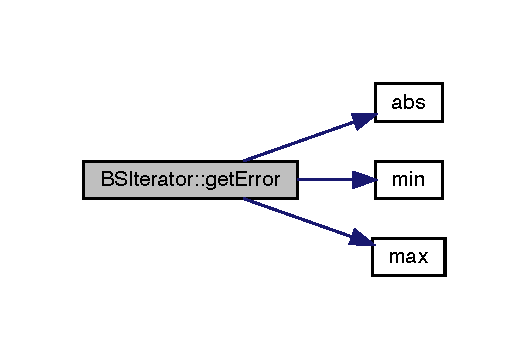
\includegraphics[width=254pt]{class_b_s_iterator_a9f50e084f8650e4d7fea3535a0547139_cgraph}
\end{center}
\end{figure}
\mbox{\Hypertarget{class_b_s_iterator_a9d06a0d0c9e458ea96952b0514adece9}\label{class_b_s_iterator_a9d06a0d0c9e458ea96952b0514adece9}} 
\index{B\+S\+Iterator@{B\+S\+Iterator}!get\+Time\+Step\+Coef@{get\+Time\+Step\+Coef}}
\index{get\+Time\+Step\+Coef@{get\+Time\+Step\+Coef}!B\+S\+Iterator@{B\+S\+Iterator}}
\paragraph{\texorpdfstring{get\+Time\+Step\+Coef()}{getTimeStepCoef()}}
{\footnotesize\ttfamily template$<$typename Partic\+Sys , typename Integrator $>$ \\
Partic\+Sys\+::\+Scalar \mbox{\hyperlink{class_b_s_iterator}{B\+S\+Iterator}}$<$ Partic\+Sys, Integrator $>$\+::get\+Time\+Step\+Coef (\begin{DoxyParamCaption}\item[{\mbox{\hyperlink{class_b_s_iterator_a7857f8ff9032955ea4dcc22cd18ca7a1}{Scalar}}}]{error,  }\item[{size\+\_\+t}]{order }\end{DoxyParamCaption})\hspace{0.3cm}{\ttfamily [private]}}



Calculate the new iteration integration step coefficient. 


\begin{DoxyParams}{Parameters}
{\em error} & The error of the k-\/th row of extrapolation table. \\
\hline
{\em order} & The order of the error in k-\/th row of extrapolation table. \\
\hline
\end{DoxyParams}
\begin{DoxyReturn}{Returns}
The new iteration integration step length coefficient. 
\end{DoxyReturn}
Here is the call graph for this function\+:\nopagebreak
\begin{figure}[H]
\begin{center}
\leavevmode
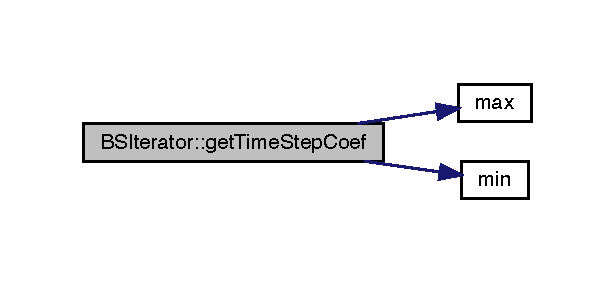
\includegraphics[width=295pt]{class_b_s_iterator_a9d06a0d0c9e458ea96952b0514adece9_cgraph}
\end{center}
\end{figure}
\mbox{\Hypertarget{class_b_s_iterator_a5520642ecbd454fb1f4d9ece18dc4e3f}\label{class_b_s_iterator_a5520642ecbd454fb1f4d9ece18dc4e3f}} 
\index{B\+S\+Iterator@{B\+S\+Iterator}!iterate@{iterate}}
\index{iterate@{iterate}!B\+S\+Iterator@{B\+S\+Iterator}}
\paragraph{\texorpdfstring{iterate()}{iterate()}}
{\footnotesize\ttfamily template$<$typename Partic\+Sys , typename Integrator $>$ \\
Partic\+Sys\+::\+Scalar \mbox{\hyperlink{class_b_s_iterator}{B\+S\+Iterator}}$<$ Partic\+Sys, Integrator $>$\+::iterate (\begin{DoxyParamCaption}\item[{Partic\+Sys \&}]{particles,  }\item[{Integrator \&}]{integrator,  }\item[{\mbox{\hyperlink{class_b_s_iterator_a7857f8ff9032955ea4dcc22cd18ca7a1}{Scalar}}}]{step\+Length }\end{DoxyParamCaption})}



Interface of O\+DE iterator. 

\begin{DoxyNote}{Note}
B\+Siterator will force use the internal mid-\/point integrator as the basic integrator.
\end{DoxyNote}

\begin{DoxyParams}{Parameters}
{\em particles} & Particle system need iteration. \\
\hline
{\em integrator} & Basica integrator used to evolve, but here BS iterator will force use internal mid-\/point integrator. \\
\hline
{\em step\+Length} & Macro integration step length. \\
\hline
\end{DoxyParams}
\begin{DoxyReturn}{Returns}
The next macro integration step length. 
\end{DoxyReturn}
\mbox{\Hypertarget{class_b_s_iterator_a738a558ddfacd9959c9438862001d7e8}\label{class_b_s_iterator_a738a558ddfacd9959c9438862001d7e8}} 
\index{B\+S\+Iterator@{B\+S\+Iterator}!prepare\+For\+New\+Iteration@{prepare\+For\+New\+Iteration}}
\index{prepare\+For\+New\+Iteration@{prepare\+For\+New\+Iteration}!B\+S\+Iterator@{B\+S\+Iterator}}
\paragraph{\texorpdfstring{prepare\+For\+New\+Iteration()}{prepareForNewIteration()}}
{\footnotesize\ttfamily template$<$typename Partic\+Sys , typename Integrator $>$ \\
Partic\+Sys\+::\+Scalar \mbox{\hyperlink{class_b_s_iterator}{B\+S\+Iterator}}$<$ Partic\+Sys, Integrator $>$\+::prepare\+For\+New\+Iteration (\begin{DoxyParamCaption}\item[{size\+\_\+t}]{k,  }\item[{bool}]{last\+Rejection }\end{DoxyParamCaption})\hspace{0.3cm}{\ttfamily [private]}}



Calculate the new iteration integration step and new iteration depth for next iteration. 


\begin{DoxyParams}{Parameters}
{\em k} & The k-\/th iteration depth. \\
\hline
{\em last\+Rejection} & The rejection status of last trail of iteration. \\
\hline
\end{DoxyParams}
\begin{DoxyReturn}{Returns}
The new iteration step length. 
\end{DoxyReturn}
Here is the call graph for this function\+:\nopagebreak
\begin{figure}[H]
\begin{center}
\leavevmode
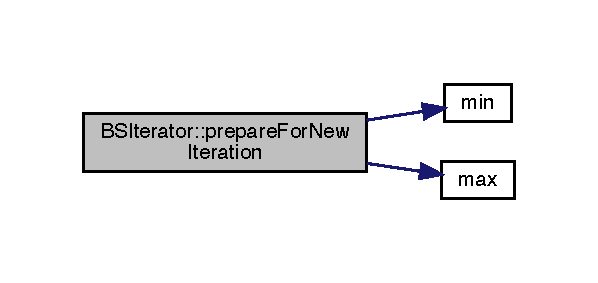
\includegraphics[width=287pt]{class_b_s_iterator_a738a558ddfacd9959c9438862001d7e8_cgraph}
\end{center}
\end{figure}
\mbox{\Hypertarget{class_b_s_iterator_a57603539823be271c2229d0951b7d957}\label{class_b_s_iterator_a57603539823be271c2229d0951b7d957}} 
\index{B\+S\+Iterator@{B\+S\+Iterator}!set\+Absolute\+Error@{set\+Absolute\+Error}}
\index{set\+Absolute\+Error@{set\+Absolute\+Error}!B\+S\+Iterator@{B\+S\+Iterator}}
\paragraph{\texorpdfstring{set\+Absolute\+Error()}{setAbsoluteError()}}
{\footnotesize\ttfamily template$<$typename Partic\+Sys , typename Integrator $>$ \\
void \mbox{\hyperlink{class_b_s_iterator}{B\+S\+Iterator}}$<$ Partic\+Sys, Integrator $>$\+::set\+Absolute\+Error (\begin{DoxyParamCaption}\item[{\mbox{\hyperlink{class_b_s_iterator_a7857f8ff9032955ea4dcc22cd18ca7a1}{Scalar}}}]{abs\+Error }\end{DoxyParamCaption})\hspace{0.3cm}{\ttfamily [inline]}}



Set the local absolute error. 

\mbox{\Hypertarget{class_b_s_iterator_ada9b6cc673e297135646699d581fcdc7}\label{class_b_s_iterator_ada9b6cc673e297135646699d581fcdc7}} 
\index{B\+S\+Iterator@{B\+S\+Iterator}!set\+Relative\+Error@{set\+Relative\+Error}}
\index{set\+Relative\+Error@{set\+Relative\+Error}!B\+S\+Iterator@{B\+S\+Iterator}}
\paragraph{\texorpdfstring{set\+Relative\+Error()}{setRelativeError()}}
{\footnotesize\ttfamily template$<$typename Partic\+Sys , typename Integrator $>$ \\
void \mbox{\hyperlink{class_b_s_iterator}{B\+S\+Iterator}}$<$ Partic\+Sys, Integrator $>$\+::set\+Relative\+Error (\begin{DoxyParamCaption}\item[{\mbox{\hyperlink{class_b_s_iterator_a7857f8ff9032955ea4dcc22cd18ca7a1}{Scalar}}}]{rel\+Error }\end{DoxyParamCaption})\hspace{0.3cm}{\ttfamily [inline]}}



Set the local relative error. 



\subsubsection{Member Data Documentation}
\mbox{\Hypertarget{class_b_s_iterator_a8948aa04b0ec390d43eb3d1f0a2efb03}\label{class_b_s_iterator_a8948aa04b0ec390d43eb3d1f0a2efb03}} 
\index{B\+S\+Iterator@{B\+S\+Iterator}!absolute\+Error@{absolute\+Error}}
\index{absolute\+Error@{absolute\+Error}!B\+S\+Iterator@{B\+S\+Iterator}}
\paragraph{\texorpdfstring{absolute\+Error}{absoluteError}}
{\footnotesize\ttfamily template$<$typename Partic\+Sys , typename Integrator $>$ \\
\mbox{\hyperlink{class_b_s_iterator_a7857f8ff9032955ea4dcc22cd18ca7a1}{Scalar}} \mbox{\hyperlink{class_b_s_iterator}{B\+S\+Iterator}}$<$ Partic\+Sys, Integrator $>$\+::absolute\+Error \{1e-\/15\}\hspace{0.3cm}{\ttfamily [private]}}



Local absolute error. 

\mbox{\Hypertarget{class_b_s_iterator_a28f6cc2fd6bfd554f85225492f4210b7}\label{class_b_s_iterator_a28f6cc2fd6bfd554f85225492f4210b7}} 
\index{B\+S\+Iterator@{B\+S\+Iterator}!CC@{CC}}
\index{CC@{CC}!B\+S\+Iterator@{B\+S\+Iterator}}
\paragraph{\texorpdfstring{CC}{CC}}
{\footnotesize\ttfamily template$<$typename Partic\+Sys , typename Integrator $>$ \\
\mbox{\hyperlink{class_b_s_iterator_ab0aa7c10b56500273af05dcd85fd8389}{scalar\+Array}}$<$ \mbox{\hyperlink{class_b_s_iterator_a7857f8ff9032955ea4dcc22cd18ca7a1}{Scalar}}, (\mbox{\hyperlink{class_b_s_iterator_a39409b9a12d4854d101ce59a0efc0f74}{Max\+Depth}} + 1)$\ast$ (\mbox{\hyperlink{class_b_s_iterator_a39409b9a12d4854d101ce59a0efc0f74}{Max\+Depth}} + 2) / 2 $>$ \mbox{\hyperlink{class_b_s_iterator}{B\+S\+Iterator}}$<$ Partic\+Sys, Integrator $>$\+::CC\hspace{0.3cm}{\ttfamily [private]}}



Extrapolation coefficient. 

\mbox{\Hypertarget{class_b_s_iterator_a53f435811c23c0ae1713df13197fc9c9}\label{class_b_s_iterator_a53f435811c23c0ae1713df13197fc9c9}} 
\index{B\+S\+Iterator@{B\+S\+Iterator}!cost@{cost}}
\index{cost@{cost}!B\+S\+Iterator@{B\+S\+Iterator}}
\paragraph{\texorpdfstring{cost}{cost}}
{\footnotesize\ttfamily template$<$typename Partic\+Sys , typename Integrator $>$ \\
\mbox{\hyperlink{class_b_s_iterator_ab0aa7c10b56500273af05dcd85fd8389}{scalar\+Array}}$<$ size\+\_\+t, \mbox{\hyperlink{class_b_s_iterator_a39409b9a12d4854d101ce59a0efc0f74}{Max\+Depth}} + 1 $>$ \mbox{\hyperlink{class_b_s_iterator}{B\+S\+Iterator}}$<$ Partic\+Sys, Integrator $>$\+::cost\hspace{0.3cm}{\ttfamily [private]}}



The work(calculation quantities) of each iteration depth. 

\mbox{\Hypertarget{class_b_s_iterator_aa501e973f342248fc445d59a5166ccc9}\label{class_b_s_iterator_aa501e973f342248fc445d59a5166ccc9}} 
\index{B\+S\+Iterator@{B\+S\+Iterator}!extrap\+Tab@{extrap\+Tab}}
\index{extrap\+Tab@{extrap\+Tab}!B\+S\+Iterator@{B\+S\+Iterator}}
\paragraph{\texorpdfstring{extrap\+Tab}{extrapTab}}
{\footnotesize\ttfamily template$<$typename Partic\+Sys , typename Integrator $>$ \\
\mbox{\hyperlink{class_b_s_iterator_ab0aa7c10b56500273af05dcd85fd8389}{scalar\+Array}}$<$ \mbox{\hyperlink{class_b_s_iterator_ab0aa7c10b56500273af05dcd85fd8389}{scalar\+Array}}$<$\mbox{\hyperlink{class_b_s_iterator_a7857f8ff9032955ea4dcc22cd18ca7a1}{Scalar}}, Partic\+Sys\+::volume()$>$, (\mbox{\hyperlink{class_b_s_iterator_a39409b9a12d4854d101ce59a0efc0f74}{Max\+Depth}} + 1)$\ast$ (\mbox{\hyperlink{class_b_s_iterator_a39409b9a12d4854d101ce59a0efc0f74}{Max\+Depth}} + 2) / 2 $>$ \mbox{\hyperlink{class_b_s_iterator}{B\+S\+Iterator}}$<$ Partic\+Sys, Integrator $>$\+::extrap\+Tab\hspace{0.3cm}{\ttfamily [private]}}



Extrapolation table. 

\mbox{\Hypertarget{class_b_s_iterator_a05bf5c727d23e47349683cda1a08ed13}\label{class_b_s_iterator_a05bf5c727d23e47349683cda1a08ed13}} 
\index{B\+S\+Iterator@{B\+S\+Iterator}!fmin@{fmin}}
\index{fmin@{fmin}!B\+S\+Iterator@{B\+S\+Iterator}}
\paragraph{\texorpdfstring{fmin}{fmin}}
{\footnotesize\ttfamily template$<$typename Partic\+Sys , typename Integrator $>$ \\
\mbox{\hyperlink{class_b_s_iterator_ab0aa7c10b56500273af05dcd85fd8389}{scalar\+Array}}$<$ \mbox{\hyperlink{class_b_s_iterator_a7857f8ff9032955ea4dcc22cd18ca7a1}{Scalar}}, \mbox{\hyperlink{class_b_s_iterator_a39409b9a12d4854d101ce59a0efc0f74}{Max\+Depth}} + 1 $>$ \mbox{\hyperlink{class_b_s_iterator}{B\+S\+Iterator}}$<$ Partic\+Sys, Integrator $>$\+::fmin\hspace{0.3cm}{\ttfamily [private]}}



The minimal coeffient of integration step estimation. 

\mbox{\Hypertarget{class_b_s_iterator_aa073f847cc5855f727c8f326f539a5f0}\label{class_b_s_iterator_aa073f847cc5855f727c8f326f539a5f0}} 
\index{B\+S\+Iterator@{B\+S\+Iterator}!iter\+Depth@{iter\+Depth}}
\index{iter\+Depth@{iter\+Depth}!B\+S\+Iterator@{B\+S\+Iterator}}
\paragraph{\texorpdfstring{iter\+Depth}{iterDepth}}
{\footnotesize\ttfamily template$<$typename Partic\+Sys , typename Integrator $>$ \\
size\+\_\+t \mbox{\hyperlink{class_b_s_iterator}{B\+S\+Iterator}}$<$ Partic\+Sys, Integrator $>$\+::iter\+Depth \{7\}\hspace{0.3cm}{\ttfamily [private]}}



Current iteraation depth. 

\mbox{\Hypertarget{class_b_s_iterator_a9d6fc5f237246465161ea86854985395}\label{class_b_s_iterator_a9d6fc5f237246465161ea86854985395}} 
\index{B\+S\+Iterator@{B\+S\+Iterator}!local\+System@{local\+System}}
\index{local\+System@{local\+System}!B\+S\+Iterator@{B\+S\+Iterator}}
\paragraph{\texorpdfstring{local\+System}{localSystem}}
{\footnotesize\ttfamily template$<$typename Partic\+Sys , typename Integrator $>$ \\
Partic\+Sys \mbox{\hyperlink{class_b_s_iterator}{B\+S\+Iterator}}$<$ Partic\+Sys, Integrator $>$\+::local\+System\hspace{0.3cm}{\ttfamily [private]}}



The local partical system used to iterate. 

\mbox{\Hypertarget{class_b_s_iterator_a96c58777cbefe7d02e160317621fc0b9}\label{class_b_s_iterator_a96c58777cbefe7d02e160317621fc0b9}} 
\index{B\+S\+Iterator@{B\+S\+Iterator}!macro\+Step\+Length@{macro\+Step\+Length}}
\index{macro\+Step\+Length@{macro\+Step\+Length}!B\+S\+Iterator@{B\+S\+Iterator}}
\paragraph{\texorpdfstring{macro\+Step\+Length}{macroStepLength}}
{\footnotesize\ttfamily template$<$typename Partic\+Sys , typename Integrator $>$ \\
\mbox{\hyperlink{class_b_s_iterator_ab0aa7c10b56500273af05dcd85fd8389}{scalar\+Array}}$<$ \mbox{\hyperlink{class_b_s_iterator_a7857f8ff9032955ea4dcc22cd18ca7a1}{Scalar}}, \mbox{\hyperlink{class_b_s_iterator_a39409b9a12d4854d101ce59a0efc0f74}{Max\+Depth}} + 1 $>$ \mbox{\hyperlink{class_b_s_iterator}{B\+S\+Iterator}}$<$ Partic\+Sys, Integrator $>$\+::macro\+Step\+Length\hspace{0.3cm}{\ttfamily [private]}}



Macro step length for different iteration depth. 

\mbox{\Hypertarget{class_b_s_iterator_a39409b9a12d4854d101ce59a0efc0f74}\label{class_b_s_iterator_a39409b9a12d4854d101ce59a0efc0f74}} 
\index{B\+S\+Iterator@{B\+S\+Iterator}!Max\+Depth@{Max\+Depth}}
\index{Max\+Depth@{Max\+Depth}!B\+S\+Iterator@{B\+S\+Iterator}}
\paragraph{\texorpdfstring{Max\+Depth}{MaxDepth}}
{\footnotesize\ttfamily template$<$typename Partic\+Sys , typename Integrator $>$ \\
const size\+\_\+t \mbox{\hyperlink{class_b_s_iterator}{B\+S\+Iterator}}$<$ Partic\+Sys, Integrator $>$\+::Max\+Depth \{8\}\hspace{0.3cm}{\ttfamily [static]}, {\ttfamily [private]}}



The Maximum iteration depth. 

\mbox{\Hypertarget{class_b_s_iterator_a9c4c8c17a759cdff694e0bd62ed249bd}\label{class_b_s_iterator_a9c4c8c17a759cdff694e0bd62ed249bd}} 
\index{B\+S\+Iterator@{B\+S\+Iterator}!n\+Steps@{n\+Steps}}
\index{n\+Steps@{n\+Steps}!B\+S\+Iterator@{B\+S\+Iterator}}
\paragraph{\texorpdfstring{n\+Steps}{nSteps}}
{\footnotesize\ttfamily template$<$typename Partic\+Sys , typename Integrator $>$ \\
\mbox{\hyperlink{class_b_s_iterator_ab0aa7c10b56500273af05dcd85fd8389}{scalar\+Array}}$<$ size\+\_\+t, \mbox{\hyperlink{class_b_s_iterator_a39409b9a12d4854d101ce59a0efc0f74}{Max\+Depth}} + 1 $>$ \mbox{\hyperlink{class_b_s_iterator}{B\+S\+Iterator}}$<$ Partic\+Sys, Integrator $>$\+::n\+Steps\hspace{0.3cm}{\ttfamily [private]}}



Steps of integration of each iteration depth. 

\mbox{\Hypertarget{class_b_s_iterator_abce71b7bac10363f7772dc848f8722b6}\label{class_b_s_iterator_abce71b7bac10363f7772dc848f8722b6}} 
\index{B\+S\+Iterator@{B\+S\+Iterator}!relative\+Error@{relative\+Error}}
\index{relative\+Error@{relative\+Error}!B\+S\+Iterator@{B\+S\+Iterator}}
\paragraph{\texorpdfstring{relative\+Error}{relativeError}}
{\footnotesize\ttfamily template$<$typename Partic\+Sys , typename Integrator $>$ \\
\mbox{\hyperlink{class_b_s_iterator_a7857f8ff9032955ea4dcc22cd18ca7a1}{Scalar}} \mbox{\hyperlink{class_b_s_iterator}{B\+S\+Iterator}}$<$ Partic\+Sys, Integrator $>$\+::relative\+Error \{1e-\/15\}\hspace{0.3cm}{\ttfamily [private]}}



Local relative error. 

\mbox{\Hypertarget{class_b_s_iterator_a942f85e00c28ef1990d1dfbed69c9e13}\label{class_b_s_iterator_a942f85e00c28ef1990d1dfbed69c9e13}} 
\index{B\+S\+Iterator@{B\+S\+Iterator}!s1@{s1}}
\index{s1@{s1}!B\+S\+Iterator@{B\+S\+Iterator}}
\paragraph{\texorpdfstring{s1}{s1}}
{\footnotesize\ttfamily template$<$typename Partic\+Sys , typename Integrator $>$ \\
\mbox{\hyperlink{class_b_s_iterator_a7857f8ff9032955ea4dcc22cd18ca7a1}{Scalar}} \mbox{\hyperlink{class_b_s_iterator}{B\+S\+Iterator}}$<$ Partic\+Sys, Integrator $>$\+::s1 \{0.\+94\}\hspace{0.3cm}{\ttfamily [private]}}



Coefficient of new step length estimation. See \char`\"{}\+Numerical recipes\char`\"{} on page 926. 

\mbox{\Hypertarget{class_b_s_iterator_ad1cdde25df6bca7a456c1908be54065f}\label{class_b_s_iterator_ad1cdde25df6bca7a456c1908be54065f}} 
\index{B\+S\+Iterator@{B\+S\+Iterator}!s2@{s2}}
\index{s2@{s2}!B\+S\+Iterator@{B\+S\+Iterator}}
\paragraph{\texorpdfstring{s2}{s2}}
{\footnotesize\ttfamily template$<$typename Partic\+Sys , typename Integrator $>$ \\
\mbox{\hyperlink{class_b_s_iterator_a7857f8ff9032955ea4dcc22cd18ca7a1}{Scalar}} \mbox{\hyperlink{class_b_s_iterator}{B\+S\+Iterator}}$<$ Partic\+Sys, Integrator $>$\+::s2 \{0.\+95\}\hspace{0.3cm}{\ttfamily [private]}}



Coefficient of new step length estimation. 

\mbox{\Hypertarget{class_b_s_iterator_a10ea0bb96f7971e9c477daef1fda6e16}\label{class_b_s_iterator_a10ea0bb96f7971e9c477daef1fda6e16}} 
\index{B\+S\+Iterator@{B\+S\+Iterator}!s3@{s3}}
\index{s3@{s3}!B\+S\+Iterator@{B\+S\+Iterator}}
\paragraph{\texorpdfstring{s3}{s3}}
{\footnotesize\ttfamily template$<$typename Partic\+Sys , typename Integrator $>$ \\
\mbox{\hyperlink{class_b_s_iterator_a7857f8ff9032955ea4dcc22cd18ca7a1}{Scalar}} \mbox{\hyperlink{class_b_s_iterator}{B\+S\+Iterator}}$<$ Partic\+Sys, Integrator $>$\+::s3 \{0.\+02\}\hspace{0.3cm}{\ttfamily [private]}}



Coefficient of new step length estimation. 

\mbox{\Hypertarget{class_b_s_iterator_a5b3bbb2d988a5d91030060508e3b4f66}\label{class_b_s_iterator_a5b3bbb2d988a5d91030060508e3b4f66}} 
\index{B\+S\+Iterator@{B\+S\+Iterator}!s4@{s4}}
\index{s4@{s4}!B\+S\+Iterator@{B\+S\+Iterator}}
\paragraph{\texorpdfstring{s4}{s4}}
{\footnotesize\ttfamily template$<$typename Partic\+Sys , typename Integrator $>$ \\
\mbox{\hyperlink{class_b_s_iterator_a7857f8ff9032955ea4dcc22cd18ca7a1}{Scalar}} \mbox{\hyperlink{class_b_s_iterator}{B\+S\+Iterator}}$<$ Partic\+Sys, Integrator $>$\+::s4 \{4.\+0\}\hspace{0.3cm}{\ttfamily [private]}}



Coefficient of new step length estimation. 

\mbox{\Hypertarget{class_b_s_iterator_ac2a338d6c3e5014d529666032d34c987}\label{class_b_s_iterator_ac2a338d6c3e5014d529666032d34c987}} 
\index{B\+S\+Iterator@{B\+S\+Iterator}!work@{work}}
\index{work@{work}!B\+S\+Iterator@{B\+S\+Iterator}}
\paragraph{\texorpdfstring{work}{work}}
{\footnotesize\ttfamily template$<$typename Partic\+Sys , typename Integrator $>$ \\
\mbox{\hyperlink{class_b_s_iterator_ab0aa7c10b56500273af05dcd85fd8389}{scalar\+Array}}$<$ \mbox{\hyperlink{class_b_s_iterator_a7857f8ff9032955ea4dcc22cd18ca7a1}{Scalar}}, \mbox{\hyperlink{class_b_s_iterator_a39409b9a12d4854d101ce59a0efc0f74}{Max\+Depth}} + 1 $>$ \mbox{\hyperlink{class_b_s_iterator}{B\+S\+Iterator}}$<$ Partic\+Sys, Integrator $>$\+::work\hspace{0.3cm}{\ttfamily [private]}}



The work(calculation quantities) per integration length of each iteration depth. 



The documentation for this class was generated from the following file\+:\begin{DoxyCompactItemize}
\item 
O\+D\+Eiterator/\mbox{\hyperlink{_b_s_iterator_8h}{B\+S\+Iterator.\+h}}\end{DoxyCompactItemize}

\hypertarget{classconst_iterator}{}\subsection{const\+Iterator$<$ Partic\+Sys, Integrator $>$ Class Template Reference}
\label{classconst_iterator}\index{const\+Iterator$<$ Partic\+Sys, Integrator $>$@{const\+Iterator$<$ Partic\+Sys, Integrator $>$}}


Most common iterator.  




{\ttfamily \#include $<$const\+Iterator.\+h$>$}

\subsubsection*{Public Types}
\begin{DoxyCompactItemize}
\item 
typedef Partic\+Sys\+::\+Scalar \mbox{\hyperlink{classconst_iterator_a7cdf84749facbb55a6a2674646f92f52}{Scalar}}
\begin{DoxyCompactList}\small\item\em interface to iterate particle system for one step \end{DoxyCompactList}\end{DoxyCompactItemize}
\subsubsection*{Public Member Functions}
\begin{DoxyCompactItemize}
\item 
\mbox{\hyperlink{classconst_iterator_a7cdf84749facbb55a6a2674646f92f52}{Scalar}} \mbox{\hyperlink{classconst_iterator_ac38af18a50fbb2aea54656f089911a48}{iterate}} (Partic\+Sys \&particles, Integrator \&integrator, \mbox{\hyperlink{classconst_iterator_a7cdf84749facbb55a6a2674646f92f52}{Scalar}} step\+Length)
\end{DoxyCompactItemize}


\subsubsection{Detailed Description}
\subsubsection*{template$<$typename Partic\+Sys, typename Integrator$>$\newline
class const\+Iterator$<$ Partic\+Sys, Integrator $>$}

Most common iterator. 

Constant iterator keep the step length constant and integrate the particle system for one step. 

\subsubsection{Member Typedef Documentation}
\mbox{\Hypertarget{classconst_iterator_a7cdf84749facbb55a6a2674646f92f52}\label{classconst_iterator_a7cdf84749facbb55a6a2674646f92f52}} 
\index{const\+Iterator@{const\+Iterator}!Scalar@{Scalar}}
\index{Scalar@{Scalar}!const\+Iterator@{const\+Iterator}}
\paragraph{\texorpdfstring{Scalar}{Scalar}}
{\footnotesize\ttfamily template$<$typename Partic\+Sys , typename Integrator $>$ \\
typedef Partic\+Sys\+::\+Scalar \mbox{\hyperlink{classconst_iterator}{const\+Iterator}}$<$ Partic\+Sys, Integrator $>$\+::\mbox{\hyperlink{classconst_iterator_a7cdf84749facbb55a6a2674646f92f52}{Scalar}}}



interface to iterate particle system for one step 


\begin{DoxyParams}{Parameters}
{\em particles} & Particle system needs evolution. \\
\hline
{\em integrator} & Integrator to integrate the particle system. \\
\hline
{\em step\+Length} & Macro step length for iteration(\+Here, the step length of the integrator). \\
\hline
\end{DoxyParams}
\begin{DoxyReturn}{Returns}
step length for next iteration. 
\end{DoxyReturn}


\subsubsection{Member Function Documentation}
\mbox{\Hypertarget{classconst_iterator_ac38af18a50fbb2aea54656f089911a48}\label{classconst_iterator_ac38af18a50fbb2aea54656f089911a48}} 
\index{const\+Iterator@{const\+Iterator}!iterate@{iterate}}
\index{iterate@{iterate}!const\+Iterator@{const\+Iterator}}
\paragraph{\texorpdfstring{iterate()}{iterate()}}
{\footnotesize\ttfamily template$<$typename Partic\+Sys , typename Integrator $>$ \\
\mbox{\hyperlink{classconst_iterator_a7cdf84749facbb55a6a2674646f92f52}{Scalar}} \mbox{\hyperlink{classconst_iterator}{const\+Iterator}}$<$ Partic\+Sys, Integrator $>$\+::iterate (\begin{DoxyParamCaption}\item[{Partic\+Sys \&}]{particles,  }\item[{Integrator \&}]{integrator,  }\item[{\mbox{\hyperlink{classconst_iterator_a7cdf84749facbb55a6a2674646f92f52}{Scalar}}}]{step\+Length }\end{DoxyParamCaption})\hspace{0.3cm}{\ttfamily [inline]}}



The documentation for this class was generated from the following file\+:\begin{DoxyCompactItemize}
\item 
O\+D\+Eiterator/\mbox{\hyperlink{const_iterator_8h}{const\+Iterator.\+h}}\end{DoxyCompactItemize}

\hypertarget{classdynamics}{}\section{dynamics$<$ Data\+Type, N $>$ Class Template Reference}
\label{classdynamics}\index{dynamics$<$ Data\+Type, N $>$@{dynamics$<$ Data\+Type, N $>$}}


Class of dynamical variable.  




{\ttfamily \#include $<$dynamic\+State.\+h$>$}

\subsection*{Public Types}
\begin{DoxyCompactItemize}
\item 
typedef Data\+Type \mbox{\hyperlink{classdynamics_a444c7534e86115117798563cb0e43cde}{Scalar}}
\item 
typedef \mbox{\hyperlink{structvec3}{vec3}}$<$ \mbox{\hyperlink{classdynamics_a444c7534e86115117798563cb0e43cde}{Scalar}} $>$ \mbox{\hyperlink{classdynamics_a9ba7c016128ac3a2eb51f7bcfbf90243}{Vector}}
\item 
typedef std\+::array$<$ \mbox{\hyperlink{structvec3}{vec3}}$<$ \mbox{\hyperlink{classdynamics_a444c7534e86115117798563cb0e43cde}{Scalar}} $>$, N $>$ \mbox{\hyperlink{classdynamics_a41e25703d6668a66d96a1db3dc5df03b}{Vector\+Array}}
\item 
typedef std\+::array$<$ \mbox{\hyperlink{classdynamics_a444c7534e86115117798563cb0e43cde}{Scalar}}, N $>$ \mbox{\hyperlink{classdynamics_ac31f831ea1577092662dafd2daba0f48}{Scalar\+Array}}
\end{DoxyCompactItemize}
\subsection*{Public Member Functions}
\begin{DoxyCompactItemize}
\item 
std\+::array$<$ \mbox{\hyperlink{classdynamics_a444c7534e86115117798563cb0e43cde}{Scalar}}, \mbox{\hyperlink{classdynamics_ada4a2418d86de3072e1a238a95e6bdb2}{volume}}()$>$ \& \mbox{\hyperlink{classdynamics_add2d27f86c6f415999e9e7dd05cc8025}{array}} ()
\begin{DoxyCompactList}\small\item\em Transfer this class to a plain array. \end{DoxyCompactList}\item 
void \mbox{\hyperlink{classdynamics_a4f6f246917f12269d3bd4a428bd40752}{init\+Addi\+Variable}} (\mbox{\hyperlink{classdynamics_ac31f831ea1577092662dafd2daba0f48}{Scalar\+Array}} \&mass)
\begin{DoxyCompactList}\small\item\em Initialize extra user defined variables. Interface required for other class. \end{DoxyCompactList}\item 
void \mbox{\hyperlink{classdynamics_a4dc0dd48fd48ef5cfc0128faaeb22b32}{set\+Zero}} ()
\begin{DoxyCompactList}\small\item\em Set all data to be zero. \end{DoxyCompactList}\end{DoxyCompactItemize}
\subsection*{Static Public Member Functions}
\begin{DoxyCompactItemize}
\item 
static constexpr size\+\_\+t \mbox{\hyperlink{classdynamics_a414656e44a6981327ae59af4deea9b8c}{size}} ()
\begin{DoxyCompactList}\small\item\em Get the number of the particles. \end{DoxyCompactList}\item 
static constexpr size\+\_\+t \mbox{\hyperlink{classdynamics_ada4a2418d86de3072e1a238a95e6bdb2}{volume}} ()
\begin{DoxyCompactList}\small\item\em Get the total data number. \end{DoxyCompactList}\end{DoxyCompactItemize}
\subsection*{Public Attributes}
\begin{DoxyCompactItemize}
\item 
\mbox{\hyperlink{classdynamics_a41e25703d6668a66d96a1db3dc5df03b}{Vector\+Array}} \mbox{\hyperlink{classdynamics_a79f983dcbf7107058280f798ab419b69}{pos}}
\begin{DoxyCompactList}\small\item\em Array of position of the particles. Element is 3D vector. \end{DoxyCompactList}\item 
\mbox{\hyperlink{classdynamics_a41e25703d6668a66d96a1db3dc5df03b}{Vector\+Array}} \mbox{\hyperlink{classdynamics_a211067eb96b01c17d2fc73d1fc65d595}{vel}}
\begin{DoxyCompactList}\small\item\em Array of velocity of the particles. Element is 3D vector. \end{DoxyCompactList}\item 
\mbox{\hyperlink{classdynamics_a444c7534e86115117798563cb0e43cde}{Scalar}} \mbox{\hyperlink{classdynamics_a95cb1723922c4224bf5d1118eed46c0c}{time}} \{0.\+0\}
\begin{DoxyCompactList}\small\item\em The physical time of the dynamic system. \end{DoxyCompactList}\end{DoxyCompactItemize}


\subsection{Detailed Description}
\subsubsection*{template$<$typename Data\+Type, size\+\_\+t N$>$\newline
class dynamics$<$ Data\+Type, N $>$}

Class of dynamical variable. 

All variables in this class are physical quantities need to be evolved. If you want to create you own dynamic state, make sure remove constant quantities away from the class. The interface \mbox{\hyperlink{classdynamics_add2d27f86c6f415999e9e7dd05cc8025}{array()}} can be used to operate the data in the class as a plain array(for evolution). Extra constant physical quantities waste the calculation. 

\subsection{Member Typedef Documentation}
\mbox{\Hypertarget{classdynamics_a444c7534e86115117798563cb0e43cde}\label{classdynamics_a444c7534e86115117798563cb0e43cde}} 
\index{dynamics@{dynamics}!Scalar@{Scalar}}
\index{Scalar@{Scalar}!dynamics@{dynamics}}
\subsubsection{\texorpdfstring{Scalar}{Scalar}}
{\footnotesize\ttfamily template$<$typename Data\+Type , size\+\_\+t N$>$ \\
typedef Data\+Type \mbox{\hyperlink{classdynamics}{dynamics}}$<$ Data\+Type, N $>$\+::\mbox{\hyperlink{classdynamics_a444c7534e86115117798563cb0e43cde}{Scalar}}}

\mbox{\Hypertarget{classdynamics_ac31f831ea1577092662dafd2daba0f48}\label{classdynamics_ac31f831ea1577092662dafd2daba0f48}} 
\index{dynamics@{dynamics}!Scalar\+Array@{Scalar\+Array}}
\index{Scalar\+Array@{Scalar\+Array}!dynamics@{dynamics}}
\subsubsection{\texorpdfstring{Scalar\+Array}{ScalarArray}}
{\footnotesize\ttfamily template$<$typename Data\+Type , size\+\_\+t N$>$ \\
typedef std\+::array$<$\mbox{\hyperlink{classdynamics_a444c7534e86115117798563cb0e43cde}{Scalar}}, N$>$ \mbox{\hyperlink{classdynamics}{dynamics}}$<$ Data\+Type, N $>$\+::\mbox{\hyperlink{classdynamics_ac31f831ea1577092662dafd2daba0f48}{Scalar\+Array}}}

\mbox{\Hypertarget{classdynamics_a9ba7c016128ac3a2eb51f7bcfbf90243}\label{classdynamics_a9ba7c016128ac3a2eb51f7bcfbf90243}} 
\index{dynamics@{dynamics}!Vector@{Vector}}
\index{Vector@{Vector}!dynamics@{dynamics}}
\subsubsection{\texorpdfstring{Vector}{Vector}}
{\footnotesize\ttfamily template$<$typename Data\+Type , size\+\_\+t N$>$ \\
typedef \mbox{\hyperlink{structvec3}{vec3}}$<$\mbox{\hyperlink{classdynamics_a444c7534e86115117798563cb0e43cde}{Scalar}}$>$ \mbox{\hyperlink{classdynamics}{dynamics}}$<$ Data\+Type, N $>$\+::\mbox{\hyperlink{classdynamics_a9ba7c016128ac3a2eb51f7bcfbf90243}{Vector}}}

\mbox{\Hypertarget{classdynamics_a41e25703d6668a66d96a1db3dc5df03b}\label{classdynamics_a41e25703d6668a66d96a1db3dc5df03b}} 
\index{dynamics@{dynamics}!Vector\+Array@{Vector\+Array}}
\index{Vector\+Array@{Vector\+Array}!dynamics@{dynamics}}
\subsubsection{\texorpdfstring{Vector\+Array}{VectorArray}}
{\footnotesize\ttfamily template$<$typename Data\+Type , size\+\_\+t N$>$ \\
typedef std\+::array$<$\mbox{\hyperlink{structvec3}{vec3}}$<$\mbox{\hyperlink{classdynamics_a444c7534e86115117798563cb0e43cde}{Scalar}}$>$, N$>$ \mbox{\hyperlink{classdynamics}{dynamics}}$<$ Data\+Type, N $>$\+::\mbox{\hyperlink{classdynamics_a41e25703d6668a66d96a1db3dc5df03b}{Vector\+Array}}}



\subsection{Member Function Documentation}
\mbox{\Hypertarget{classdynamics_add2d27f86c6f415999e9e7dd05cc8025}\label{classdynamics_add2d27f86c6f415999e9e7dd05cc8025}} 
\index{dynamics@{dynamics}!array@{array}}
\index{array@{array}!dynamics@{dynamics}}
\subsubsection{\texorpdfstring{array()}{array()}}
{\footnotesize\ttfamily template$<$typename Data\+Type , size\+\_\+t N$>$ \\
std\+::array$<$\mbox{\hyperlink{classdynamics_a444c7534e86115117798563cb0e43cde}{Scalar}}, \mbox{\hyperlink{classdynamics_ada4a2418d86de3072e1a238a95e6bdb2}{volume}}()$>$\& \mbox{\hyperlink{classdynamics}{dynamics}}$<$ Data\+Type, N $>$\+::array (\begin{DoxyParamCaption}{ }\end{DoxyParamCaption})\hspace{0.3cm}{\ttfamily [inline]}}



Transfer this class to a plain array. 

\begin{DoxyReturn}{Returns}
The reference of head of this class, reinterpret as a plain array. 
\end{DoxyReturn}
\mbox{\Hypertarget{classdynamics_a4f6f246917f12269d3bd4a428bd40752}\label{classdynamics_a4f6f246917f12269d3bd4a428bd40752}} 
\index{dynamics@{dynamics}!init\+Addi\+Variable@{init\+Addi\+Variable}}
\index{init\+Addi\+Variable@{init\+Addi\+Variable}!dynamics@{dynamics}}
\subsubsection{\texorpdfstring{init\+Addi\+Variable()}{initAddiVariable()}}
{\footnotesize\ttfamily template$<$typename Data\+Type , size\+\_\+t N$>$ \\
void \mbox{\hyperlink{classdynamics}{dynamics}}$<$ Data\+Type, N $>$\+::init\+Addi\+Variable (\begin{DoxyParamCaption}\item[{\mbox{\hyperlink{classdynamics_ac31f831ea1577092662dafd2daba0f48}{Scalar\+Array}} \&}]{mass }\end{DoxyParamCaption})\hspace{0.3cm}{\ttfamily [inline]}}



Initialize extra user defined variables. Interface required for other class. 


\begin{DoxyParams}{Parameters}
{\em mass} & The mass of particles, might be required for initialization. \\
\hline
\end{DoxyParams}
\mbox{\Hypertarget{classdynamics_a4dc0dd48fd48ef5cfc0128faaeb22b32}\label{classdynamics_a4dc0dd48fd48ef5cfc0128faaeb22b32}} 
\index{dynamics@{dynamics}!set\+Zero@{set\+Zero}}
\index{set\+Zero@{set\+Zero}!dynamics@{dynamics}}
\subsubsection{\texorpdfstring{set\+Zero()}{setZero()}}
{\footnotesize\ttfamily template$<$typename Data\+Type , size\+\_\+t N$>$ \\
void \mbox{\hyperlink{classdynamics}{dynamics}}$<$ Data\+Type, N $>$\+::set\+Zero (\begin{DoxyParamCaption}{ }\end{DoxyParamCaption})\hspace{0.3cm}{\ttfamily [inline]}}



Set all data to be zero. 

Here is the call graph for this function\+:\nopagebreak
\begin{figure}[H]
\begin{center}
\leavevmode
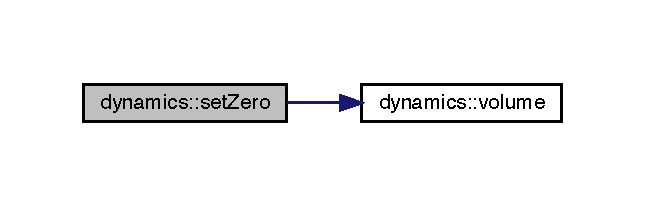
\includegraphics[width=310pt]{classdynamics_a4dc0dd48fd48ef5cfc0128faaeb22b32_cgraph}
\end{center}
\end{figure}
\mbox{\Hypertarget{classdynamics_a414656e44a6981327ae59af4deea9b8c}\label{classdynamics_a414656e44a6981327ae59af4deea9b8c}} 
\index{dynamics@{dynamics}!size@{size}}
\index{size@{size}!dynamics@{dynamics}}
\subsubsection{\texorpdfstring{size()}{size()}}
{\footnotesize\ttfamily template$<$typename Data\+Type , size\+\_\+t N$>$ \\
static constexpr size\+\_\+t \mbox{\hyperlink{classdynamics}{dynamics}}$<$ Data\+Type, N $>$\+::size (\begin{DoxyParamCaption}{ }\end{DoxyParamCaption})\hspace{0.3cm}{\ttfamily [inline]}, {\ttfamily [static]}}



Get the number of the particles. 

\begin{DoxyReturn}{Returns}
The particle number. 
\end{DoxyReturn}
\mbox{\Hypertarget{classdynamics_ada4a2418d86de3072e1a238a95e6bdb2}\label{classdynamics_ada4a2418d86de3072e1a238a95e6bdb2}} 
\index{dynamics@{dynamics}!volume@{volume}}
\index{volume@{volume}!dynamics@{dynamics}}
\subsubsection{\texorpdfstring{volume()}{volume()}}
{\footnotesize\ttfamily template$<$typename Data\+Type , size\+\_\+t N$>$ \\
static constexpr size\+\_\+t \mbox{\hyperlink{classdynamics}{dynamics}}$<$ Data\+Type, N $>$\+::volume (\begin{DoxyParamCaption}{ }\end{DoxyParamCaption})\hspace{0.3cm}{\ttfamily [inline]}, {\ttfamily [static]}}



Get the total data number. 

\begin{DoxyReturn}{Returns}
The data number. 
\end{DoxyReturn}
Here is the caller graph for this function\+:\nopagebreak
\begin{figure}[H]
\begin{center}
\leavevmode
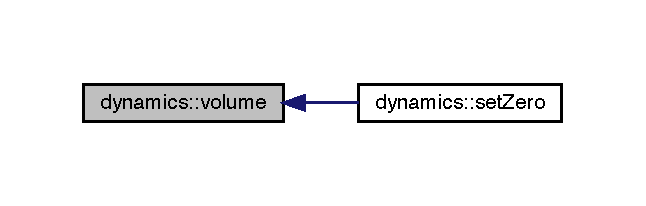
\includegraphics[width=310pt]{classdynamics_ada4a2418d86de3072e1a238a95e6bdb2_icgraph}
\end{center}
\end{figure}


\subsection{Member Data Documentation}
\mbox{\Hypertarget{classdynamics_a79f983dcbf7107058280f798ab419b69}\label{classdynamics_a79f983dcbf7107058280f798ab419b69}} 
\index{dynamics@{dynamics}!pos@{pos}}
\index{pos@{pos}!dynamics@{dynamics}}
\subsubsection{\texorpdfstring{pos}{pos}}
{\footnotesize\ttfamily template$<$typename Data\+Type , size\+\_\+t N$>$ \\
\mbox{\hyperlink{classdynamics_a41e25703d6668a66d96a1db3dc5df03b}{Vector\+Array}} \mbox{\hyperlink{classdynamics}{dynamics}}$<$ Data\+Type, N $>$\+::pos}



Array of position of the particles. Element is 3D vector. 

\mbox{\Hypertarget{classdynamics_a95cb1723922c4224bf5d1118eed46c0c}\label{classdynamics_a95cb1723922c4224bf5d1118eed46c0c}} 
\index{dynamics@{dynamics}!time@{time}}
\index{time@{time}!dynamics@{dynamics}}
\subsubsection{\texorpdfstring{time}{time}}
{\footnotesize\ttfamily template$<$typename Data\+Type , size\+\_\+t N$>$ \\
\mbox{\hyperlink{classdynamics_a444c7534e86115117798563cb0e43cde}{Scalar}} \mbox{\hyperlink{classdynamics}{dynamics}}$<$ Data\+Type, N $>$\+::time \{0.\+0\}}



The physical time of the dynamic system. 

\mbox{\Hypertarget{classdynamics_a211067eb96b01c17d2fc73d1fc65d595}\label{classdynamics_a211067eb96b01c17d2fc73d1fc65d595}} 
\index{dynamics@{dynamics}!vel@{vel}}
\index{vel@{vel}!dynamics@{dynamics}}
\subsubsection{\texorpdfstring{vel}{vel}}
{\footnotesize\ttfamily template$<$typename Data\+Type , size\+\_\+t N$>$ \\
\mbox{\hyperlink{classdynamics_a41e25703d6668a66d96a1db3dc5df03b}{Vector\+Array}} \mbox{\hyperlink{classdynamics}{dynamics}}$<$ Data\+Type, N $>$\+::vel}



Array of velocity of the particles. Element is 3D vector. 



The documentation for this class was generated from the following file\+:\begin{DoxyCompactItemize}
\item 
\mbox{\hyperlink{dynamic_state_8h}{dynamic\+State.\+h}}\end{DoxyCompactItemize}

\hypertarget{classdynamic_system}{}\section{dynamic\+System$<$ Partic\+Sys, O\+D\+Eiterator $>$ Class Template Reference}
\label{classdynamic_system}\index{dynamic\+System$<$ Partic\+Sys, O\+D\+Eiterator $>$@{dynamic\+System$<$ Partic\+Sys, O\+D\+Eiterator $>$}}


A wrapper to make particle system, integrator and O\+DE iterator work together.  




{\ttfamily \#include $<$dynamic\+System.\+h$>$}

\subsection*{Public Types}
\begin{DoxyCompactItemize}
\item 
using \mbox{\hyperlink{classdynamic_system_a518990ebef8f3f6257e6ef0e49fe013e}{type}} = typename Partic\+Sys\+::type
\item 
using \mbox{\hyperlink{classdynamic_system_a6eb7b06a4ee5721a1ee0855a854c3431}{Scalar}} = typename type\+::\+Scalar
\end{DoxyCompactItemize}
\subsection*{Public Member Functions}
\begin{DoxyCompactItemize}
\item 
void \mbox{\hyperlink{classdynamic_system_a7a4032c043dd0286007f4d7c542d3f95}{advance\+One\+Step}} ()
\begin{DoxyCompactList}\small\item\em Advance the particle system for one step. \end{DoxyCompactList}\item 
void \mbox{\hyperlink{classdynamic_system_a3ff4342241733e94edce17c1a79a90a8}{load\+Text}} (char const $\ast$init\+File\+Path)
\begin{DoxyCompactList}\small\item\em Load particle system initial condition from file. \end{DoxyCompactList}\item 
void \mbox{\hyperlink{classdynamic_system_a0392d5b36a03692d65616f3b40168948}{set\+Step\+Length}} (\mbox{\hyperlink{classdynamic_system_a6eb7b06a4ee5721a1ee0855a854c3431}{Scalar}})
\begin{DoxyCompactList}\small\item\em Set the step length. \end{DoxyCompactList}\item 
virtual \mbox{\hyperlink{classdynamic_system_a239af38fcf35f3fe32d5ae5e183e4cca}{$\sim$dynamic\+System}} ()
\begin{DoxyCompactList}\small\item\em Default destructor, virtualize for inherent class. \end{DoxyCompactList}\end{DoxyCompactItemize}
\subsection*{Public Attributes}
\begin{DoxyCompactItemize}
\item 
\mbox{\hyperlink{classdynamic_system_a6eb7b06a4ee5721a1ee0855a854c3431}{Scalar}} \mbox{\hyperlink{classdynamic_system_a3f0e5b7ef17b728c723c67aefa9dbada}{step\+Length}} \{0.\+0\}
\begin{DoxyCompactList}\small\item\em Macro step size for O\+DE iterator. \end{DoxyCompactList}\item 
int \mbox{\hyperlink{classdynamic_system_ae9821e179896e6cddbbcc4e706552c57}{steps}} \{0\}
\begin{DoxyCompactList}\small\item\em Steps. \end{DoxyCompactList}\item 
Partic\+Sys \mbox{\hyperlink{classdynamic_system_a809657c0ef63741a7e3d6f32bc87bfe3}{particles}}
\begin{DoxyCompactList}\small\item\em Particle system. \end{DoxyCompactList}\item 
O\+D\+Eiterator \mbox{\hyperlink{classdynamic_system_a0a13a11664ce5761ab4296b1b0421f99}{iterator}}
\begin{DoxyCompactList}\small\item\em O\+DE Iterator. \end{DoxyCompactList}\end{DoxyCompactItemize}


\subsection{Detailed Description}
\subsubsection*{template$<$typename Partic\+Sys, typename O\+D\+Eiterator$>$\newline
class dynamic\+System$<$ Partic\+Sys, O\+D\+Eiterator $>$}

A wrapper to make particle system, integrator and O\+DE iterator work together. 

Definition at line 31 of file dynamic\+System.\+h.



\subsection{Member Typedef Documentation}
\mbox{\Hypertarget{classdynamic_system_a6eb7b06a4ee5721a1ee0855a854c3431}\label{classdynamic_system_a6eb7b06a4ee5721a1ee0855a854c3431}} 
\index{dynamic\+System@{dynamic\+System}!Scalar@{Scalar}}
\index{Scalar@{Scalar}!dynamic\+System@{dynamic\+System}}
\subsubsection{\texorpdfstring{Scalar}{Scalar}}
{\footnotesize\ttfamily template$<$typename Partic\+Sys , typename O\+D\+Eiterator $>$ \\
using \mbox{\hyperlink{classdynamic_system}{dynamic\+System}}$<$ Partic\+Sys, O\+D\+Eiterator $>$\+::\mbox{\hyperlink{classdynamic_system_a6eb7b06a4ee5721a1ee0855a854c3431}{Scalar}} =  typename type\+::\+Scalar}



Definition at line 35 of file dynamic\+System.\+h.

\mbox{\Hypertarget{classdynamic_system_a518990ebef8f3f6257e6ef0e49fe013e}\label{classdynamic_system_a518990ebef8f3f6257e6ef0e49fe013e}} 
\index{dynamic\+System@{dynamic\+System}!type@{type}}
\index{type@{type}!dynamic\+System@{dynamic\+System}}
\subsubsection{\texorpdfstring{type}{type}}
{\footnotesize\ttfamily template$<$typename Partic\+Sys , typename O\+D\+Eiterator $>$ \\
using \mbox{\hyperlink{classdynamic_system}{dynamic\+System}}$<$ Partic\+Sys, O\+D\+Eiterator $>$\+::\mbox{\hyperlink{classdynamic_system_a518990ebef8f3f6257e6ef0e49fe013e}{type}} =  typename Partic\+Sys\+::type}



Definition at line 34 of file dynamic\+System.\+h.



\subsection{Constructor \& Destructor Documentation}
\mbox{\Hypertarget{classdynamic_system_a239af38fcf35f3fe32d5ae5e183e4cca}\label{classdynamic_system_a239af38fcf35f3fe32d5ae5e183e4cca}} 
\index{dynamic\+System@{dynamic\+System}!````~dynamic\+System@{$\sim$dynamic\+System}}
\index{````~dynamic\+System@{$\sim$dynamic\+System}!dynamic\+System@{dynamic\+System}}
\subsubsection{\texorpdfstring{$\sim$dynamic\+System()}{~dynamicSystem()}}
{\footnotesize\ttfamily template$<$typename Partic\+Sys , typename O\+D\+Eiterator $>$ \\
virtual \mbox{\hyperlink{classdynamic_system}{dynamic\+System}}$<$ Partic\+Sys, O\+D\+Eiterator $>$\+::$\sim$\mbox{\hyperlink{classdynamic_system}{dynamic\+System}} (\begin{DoxyParamCaption}{ }\end{DoxyParamCaption})\hspace{0.3cm}{\ttfamily [inline]}, {\ttfamily [virtual]}}



Default destructor, virtualize for inherent class. 



Definition at line 40 of file dynamic\+System.\+h.



\subsection{Member Function Documentation}
\mbox{\Hypertarget{classdynamic_system_a7a4032c043dd0286007f4d7c542d3f95}\label{classdynamic_system_a7a4032c043dd0286007f4d7c542d3f95}} 
\index{dynamic\+System@{dynamic\+System}!advance\+One\+Step@{advance\+One\+Step}}
\index{advance\+One\+Step@{advance\+One\+Step}!dynamic\+System@{dynamic\+System}}
\subsubsection{\texorpdfstring{advance\+One\+Step()}{advanceOneStep()}}
{\footnotesize\ttfamily template$<$typename Partic\+Sys , typename O\+D\+Eiterator $>$ \\
void \mbox{\hyperlink{classdynamic_system}{dynamic\+System}}$<$ Partic\+Sys, O\+D\+Eiterator $>$\+::advance\+One\+Step (\begin{DoxyParamCaption}{ }\end{DoxyParamCaption})\hspace{0.3cm}{\ttfamily [inline]}}



Advance the particle system for one step. 

Advance the particle system with current steplength step\+Length. The O\+DE iterator iterate the integrator to convergence by its own implement. The step length will also be updated by its own implement. 

Definition at line 65 of file dynamic\+System.\+h.

\mbox{\Hypertarget{classdynamic_system_a3ff4342241733e94edce17c1a79a90a8}\label{classdynamic_system_a3ff4342241733e94edce17c1a79a90a8}} 
\index{dynamic\+System@{dynamic\+System}!load\+Text@{load\+Text}}
\index{load\+Text@{load\+Text}!dynamic\+System@{dynamic\+System}}
\subsubsection{\texorpdfstring{load\+Text()}{loadText()}}
{\footnotesize\ttfamily template$<$typename Partic\+Sys , typename O\+D\+Eiterator $>$ \\
void \mbox{\hyperlink{classdynamic_system}{dynamic\+System}}$<$ Partic\+Sys, O\+D\+Eiterator $>$\+::load\+Text (\begin{DoxyParamCaption}\item[{char const $\ast$}]{init\+File\+Path }\end{DoxyParamCaption})}



Load particle system initial condition from file. 

This function will read and check the initial file header (begin with \textquotesingle{}\#\textquotesingle{}) and the particle number after the \textquotesingle{}\#\textquotesingle{}. Pass the rest information to particles by operator \textquotesingle{}$>$$>$\textquotesingle{}. The way to load the initial condition depend on the implemet of the particles. If the initial condition read successfully. This function will call get\+Init\+Step\+Length() to set the initial step length.


\begin{DoxyParams}{Parameters}
{\em init\+File\+Path} & The relative path of initial conditions file \\
\hline
\end{DoxyParams}

\begin{DoxyExceptions}{Exceptions}
{\em If} & the partcile number in the header is inconsisitent with the size of particles, this function will throw an exception. \\
\hline
\end{DoxyExceptions}


Definition at line 103 of file dynamic\+System.\+h.

Here is the caller graph for this function\+:\nopagebreak
\begin{figure}[H]
\begin{center}
\leavevmode
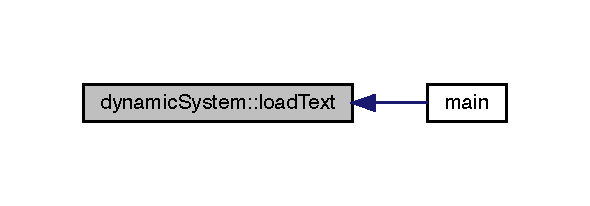
\includegraphics[width=283pt]{classdynamic_system_a3ff4342241733e94edce17c1a79a90a8_icgraph}
\end{center}
\end{figure}
\mbox{\Hypertarget{classdynamic_system_a0392d5b36a03692d65616f3b40168948}\label{classdynamic_system_a0392d5b36a03692d65616f3b40168948}} 
\index{dynamic\+System@{dynamic\+System}!set\+Step\+Length@{set\+Step\+Length}}
\index{set\+Step\+Length@{set\+Step\+Length}!dynamic\+System@{dynamic\+System}}
\subsubsection{\texorpdfstring{set\+Step\+Length()}{setStepLength()}}
{\footnotesize\ttfamily template$<$typename Partic\+Sys , typename O\+D\+Eiterator $>$ \\
void \mbox{\hyperlink{classdynamic_system}{dynamic\+System}}$<$ Partic\+Sys, O\+D\+Eiterator $>$\+::set\+Step\+Length (\begin{DoxyParamCaption}\item[{\mbox{\hyperlink{classdynamic_system_a6eb7b06a4ee5721a1ee0855a854c3431}{Scalar}}}]{step\+Size }\end{DoxyParamCaption})}



Set the step length. 



Definition at line 132 of file dynamic\+System.\+h.



\subsection{Member Data Documentation}
\mbox{\Hypertarget{classdynamic_system_a0a13a11664ce5761ab4296b1b0421f99}\label{classdynamic_system_a0a13a11664ce5761ab4296b1b0421f99}} 
\index{dynamic\+System@{dynamic\+System}!iterator@{iterator}}
\index{iterator@{iterator}!dynamic\+System@{dynamic\+System}}
\subsubsection{\texorpdfstring{iterator}{iterator}}
{\footnotesize\ttfamily template$<$typename Partic\+Sys , typename O\+D\+Eiterator $>$ \\
O\+D\+Eiterator \mbox{\hyperlink{classdynamic_system}{dynamic\+System}}$<$ Partic\+Sys, O\+D\+Eiterator $>$\+::iterator}



O\+DE Iterator. 



Definition at line 52 of file dynamic\+System.\+h.

\mbox{\Hypertarget{classdynamic_system_a809657c0ef63741a7e3d6f32bc87bfe3}\label{classdynamic_system_a809657c0ef63741a7e3d6f32bc87bfe3}} 
\index{dynamic\+System@{dynamic\+System}!particles@{particles}}
\index{particles@{particles}!dynamic\+System@{dynamic\+System}}
\subsubsection{\texorpdfstring{particles}{particles}}
{\footnotesize\ttfamily template$<$typename Partic\+Sys , typename O\+D\+Eiterator $>$ \\
Partic\+Sys \mbox{\hyperlink{classdynamic_system}{dynamic\+System}}$<$ Partic\+Sys, O\+D\+Eiterator $>$\+::particles}



Particle system. 



Definition at line 49 of file dynamic\+System.\+h.

\mbox{\Hypertarget{classdynamic_system_a3f0e5b7ef17b728c723c67aefa9dbada}\label{classdynamic_system_a3f0e5b7ef17b728c723c67aefa9dbada}} 
\index{dynamic\+System@{dynamic\+System}!step\+Length@{step\+Length}}
\index{step\+Length@{step\+Length}!dynamic\+System@{dynamic\+System}}
\subsubsection{\texorpdfstring{step\+Length}{stepLength}}
{\footnotesize\ttfamily template$<$typename Partic\+Sys , typename O\+D\+Eiterator $>$ \\
\mbox{\hyperlink{classdynamic_system_a6eb7b06a4ee5721a1ee0855a854c3431}{Scalar}} \mbox{\hyperlink{classdynamic_system}{dynamic\+System}}$<$ Partic\+Sys, O\+D\+Eiterator $>$\+::step\+Length \{0.\+0\}}



Macro step size for O\+DE iterator. 



Definition at line 43 of file dynamic\+System.\+h.

\mbox{\Hypertarget{classdynamic_system_ae9821e179896e6cddbbcc4e706552c57}\label{classdynamic_system_ae9821e179896e6cddbbcc4e706552c57}} 
\index{dynamic\+System@{dynamic\+System}!steps@{steps}}
\index{steps@{steps}!dynamic\+System@{dynamic\+System}}
\subsubsection{\texorpdfstring{steps}{steps}}
{\footnotesize\ttfamily template$<$typename Partic\+Sys , typename O\+D\+Eiterator $>$ \\
int \mbox{\hyperlink{classdynamic_system}{dynamic\+System}}$<$ Partic\+Sys, O\+D\+Eiterator $>$\+::steps \{0\}}



Steps. 



Definition at line 46 of file dynamic\+System.\+h.



The documentation for this class was generated from the following file\+:\begin{DoxyCompactItemize}
\item 
\mbox{\hyperlink{dynamic_system_8h}{dynamic\+System.\+h}}\end{DoxyCompactItemize}

\hypertarget{classerrhand}{}\subsection{errhand Class Reference}
\label{classerrhand}\index{errhand@{errhand}}


{\ttfamily \#include $<$errhand.\+h$>$}

\subsubsection*{Public Member Functions}
\begin{DoxyCompactItemize}
\item 
\mbox{\hyperlink{classerrhand_a69afd61e0ebf5ee9d35f297dc2d5c086}{errhand}} (std\+::string err\+\_\+msg\+\_\+input, const char $\ast$file\+\_\+input, size\+\_\+t line\+\_\+input)
\item 
std\+::string \mbox{\hyperlink{classerrhand_a524dfc6821f703329d8801dd3298f33f}{get\+\_\+msg}} () const
\item 
std\+::string \mbox{\hyperlink{classerrhand_a1556ee8d0aaefeea3bbab73f7ae50914}{get\+\_\+file}} () const
\item 
size\+\_\+t \mbox{\hyperlink{classerrhand_a258f97d84476b21efc38827cda3e5889}{get\+\_\+line}} () const
\item 
std\+::string \mbox{\hyperlink{classerrhand_a930df1c197154853159683cb2ad55369}{to\+\_\+string\+\_\+loc}} (const char $\ast$obj)
\item 
void \mbox{\hyperlink{classerrhand_adbc86e81b391a68d2bf9a13529c977d3}{invoke\+\_\+telegram\+\_\+bot}} ()
\item 
void \mbox{\hyperlink{classerrhand_a5b4d8a74f1d0c6842526dc8b54e38dc2}{print\+\_\+to\+\_\+stdout}} ()
\end{DoxyCompactItemize}
\subsubsection*{Private Attributes}
\begin{DoxyCompactItemize}
\item 
std\+::string \mbox{\hyperlink{classerrhand_a2baa975c76a80afce9c97575c549058c}{err\+\_\+msg}}
\item 
std\+::string \mbox{\hyperlink{classerrhand_aed73d7a312fae4b4387d8d2487277a74}{file}}
\item 
size\+\_\+t \mbox{\hyperlink{classerrhand_a3ddc204c758b97e7d1550019e4513f3b}{line}}
\end{DoxyCompactItemize}


\subsubsection{Constructor \& Destructor Documentation}
\mbox{\Hypertarget{classerrhand_a69afd61e0ebf5ee9d35f297dc2d5c086}\label{classerrhand_a69afd61e0ebf5ee9d35f297dc2d5c086}} 
\index{errhand@{errhand}!errhand@{errhand}}
\index{errhand@{errhand}!errhand@{errhand}}
\paragraph{\texorpdfstring{errhand()}{errhand()}}
{\footnotesize\ttfamily errhand\+::errhand (\begin{DoxyParamCaption}\item[{std\+::string}]{err\+\_\+msg\+\_\+input,  }\item[{const char $\ast$}]{file\+\_\+input,  }\item[{size\+\_\+t}]{line\+\_\+input }\end{DoxyParamCaption})\hspace{0.3cm}{\ttfamily [inline]}}

Here is the call graph for this function\+:\nopagebreak
\begin{figure}[H]
\begin{center}
\leavevmode
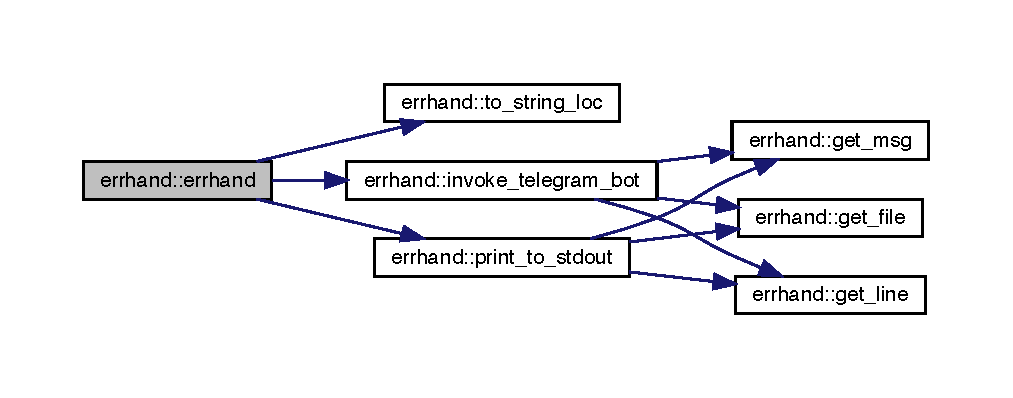
\includegraphics[width=350pt]{classerrhand_a69afd61e0ebf5ee9d35f297dc2d5c086_cgraph}
\end{center}
\end{figure}


\subsubsection{Member Function Documentation}
\mbox{\Hypertarget{classerrhand_a1556ee8d0aaefeea3bbab73f7ae50914}\label{classerrhand_a1556ee8d0aaefeea3bbab73f7ae50914}} 
\index{errhand@{errhand}!get\+\_\+file@{get\+\_\+file}}
\index{get\+\_\+file@{get\+\_\+file}!errhand@{errhand}}
\paragraph{\texorpdfstring{get\+\_\+file()}{get\_file()}}
{\footnotesize\ttfamily std\+::string errhand\+::get\+\_\+file (\begin{DoxyParamCaption}{ }\end{DoxyParamCaption}) const\hspace{0.3cm}{\ttfamily [inline]}}

Here is the caller graph for this function\+:\nopagebreak
\begin{figure}[H]
\begin{center}
\leavevmode
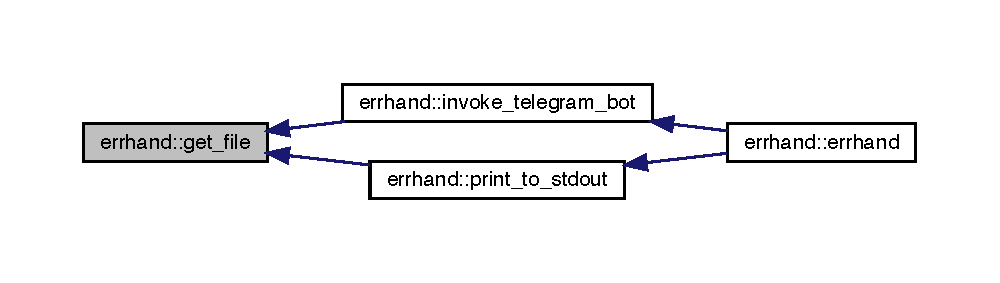
\includegraphics[width=350pt]{classerrhand_a1556ee8d0aaefeea3bbab73f7ae50914_icgraph}
\end{center}
\end{figure}
\mbox{\Hypertarget{classerrhand_a258f97d84476b21efc38827cda3e5889}\label{classerrhand_a258f97d84476b21efc38827cda3e5889}} 
\index{errhand@{errhand}!get\+\_\+line@{get\+\_\+line}}
\index{get\+\_\+line@{get\+\_\+line}!errhand@{errhand}}
\paragraph{\texorpdfstring{get\+\_\+line()}{get\_line()}}
{\footnotesize\ttfamily size\+\_\+t errhand\+::get\+\_\+line (\begin{DoxyParamCaption}{ }\end{DoxyParamCaption}) const\hspace{0.3cm}{\ttfamily [inline]}}

Here is the caller graph for this function\+:\nopagebreak
\begin{figure}[H]
\begin{center}
\leavevmode
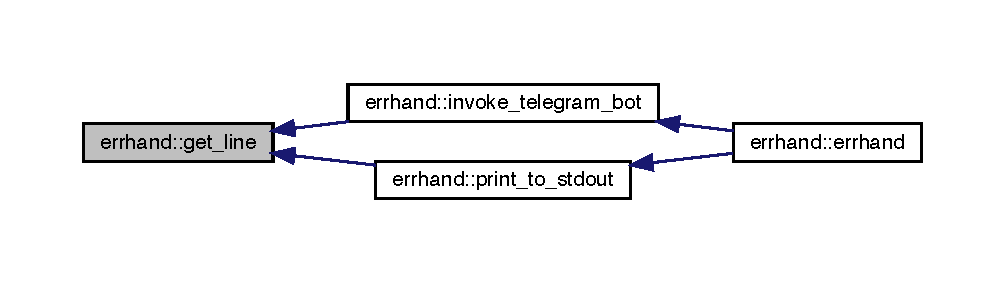
\includegraphics[width=350pt]{classerrhand_a258f97d84476b21efc38827cda3e5889_icgraph}
\end{center}
\end{figure}
\mbox{\Hypertarget{classerrhand_a524dfc6821f703329d8801dd3298f33f}\label{classerrhand_a524dfc6821f703329d8801dd3298f33f}} 
\index{errhand@{errhand}!get\+\_\+msg@{get\+\_\+msg}}
\index{get\+\_\+msg@{get\+\_\+msg}!errhand@{errhand}}
\paragraph{\texorpdfstring{get\+\_\+msg()}{get\_msg()}}
{\footnotesize\ttfamily std\+::string errhand\+::get\+\_\+msg (\begin{DoxyParamCaption}{ }\end{DoxyParamCaption}) const\hspace{0.3cm}{\ttfamily [inline]}}

Here is the caller graph for this function\+:\nopagebreak
\begin{figure}[H]
\begin{center}
\leavevmode
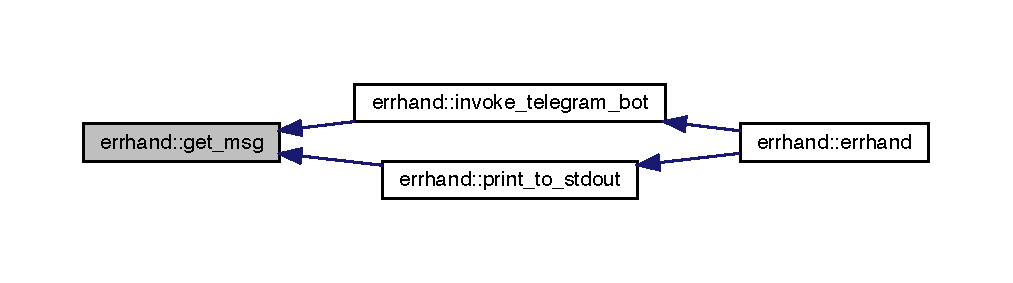
\includegraphics[width=350pt]{classerrhand_a524dfc6821f703329d8801dd3298f33f_icgraph}
\end{center}
\end{figure}
\mbox{\Hypertarget{classerrhand_adbc86e81b391a68d2bf9a13529c977d3}\label{classerrhand_adbc86e81b391a68d2bf9a13529c977d3}} 
\index{errhand@{errhand}!invoke\+\_\+telegram\+\_\+bot@{invoke\+\_\+telegram\+\_\+bot}}
\index{invoke\+\_\+telegram\+\_\+bot@{invoke\+\_\+telegram\+\_\+bot}!errhand@{errhand}}
\paragraph{\texorpdfstring{invoke\+\_\+telegram\+\_\+bot()}{invoke\_telegram\_bot()}}
{\footnotesize\ttfamily void errhand\+::invoke\+\_\+telegram\+\_\+bot (\begin{DoxyParamCaption}{ }\end{DoxyParamCaption})\hspace{0.3cm}{\ttfamily [inline]}}

Here is the call graph for this function\+:\nopagebreak
\begin{figure}[H]
\begin{center}
\leavevmode
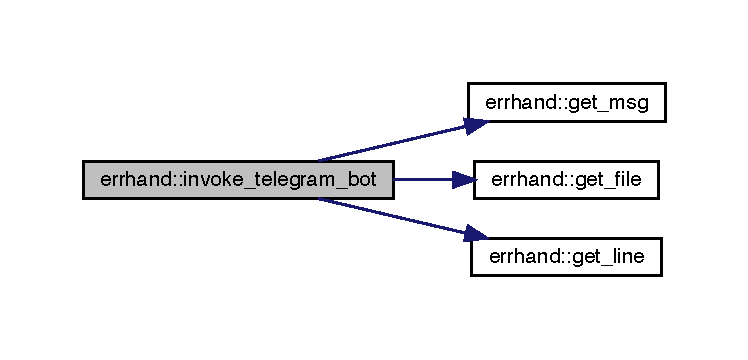
\includegraphics[width=350pt]{classerrhand_adbc86e81b391a68d2bf9a13529c977d3_cgraph}
\end{center}
\end{figure}
Here is the caller graph for this function\+:\nopagebreak
\begin{figure}[H]
\begin{center}
\leavevmode
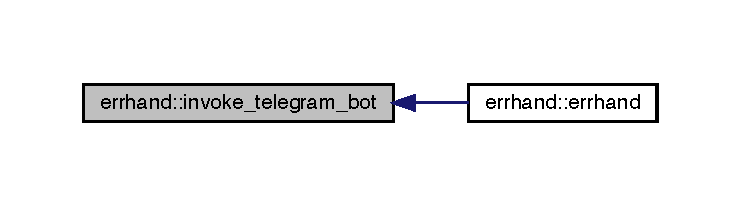
\includegraphics[width=350pt]{classerrhand_adbc86e81b391a68d2bf9a13529c977d3_icgraph}
\end{center}
\end{figure}
\mbox{\Hypertarget{classerrhand_a5b4d8a74f1d0c6842526dc8b54e38dc2}\label{classerrhand_a5b4d8a74f1d0c6842526dc8b54e38dc2}} 
\index{errhand@{errhand}!print\+\_\+to\+\_\+stdout@{print\+\_\+to\+\_\+stdout}}
\index{print\+\_\+to\+\_\+stdout@{print\+\_\+to\+\_\+stdout}!errhand@{errhand}}
\paragraph{\texorpdfstring{print\+\_\+to\+\_\+stdout()}{print\_to\_stdout()}}
{\footnotesize\ttfamily void errhand\+::print\+\_\+to\+\_\+stdout (\begin{DoxyParamCaption}{ }\end{DoxyParamCaption})\hspace{0.3cm}{\ttfamily [inline]}}

Here is the call graph for this function\+:\nopagebreak
\begin{figure}[H]
\begin{center}
\leavevmode
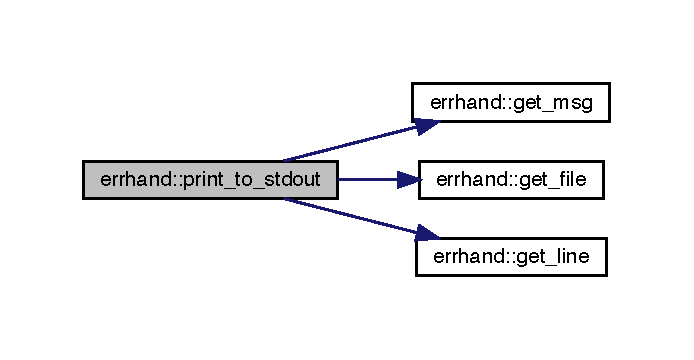
\includegraphics[width=333pt]{classerrhand_a5b4d8a74f1d0c6842526dc8b54e38dc2_cgraph}
\end{center}
\end{figure}
Here is the caller graph for this function\+:\nopagebreak
\begin{figure}[H]
\begin{center}
\leavevmode
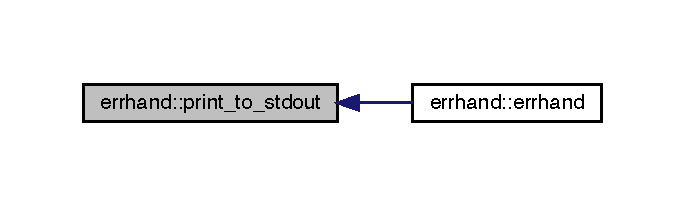
\includegraphics[width=329pt]{classerrhand_a5b4d8a74f1d0c6842526dc8b54e38dc2_icgraph}
\end{center}
\end{figure}
\mbox{\Hypertarget{classerrhand_a930df1c197154853159683cb2ad55369}\label{classerrhand_a930df1c197154853159683cb2ad55369}} 
\index{errhand@{errhand}!to\+\_\+string\+\_\+loc@{to\+\_\+string\+\_\+loc}}
\index{to\+\_\+string\+\_\+loc@{to\+\_\+string\+\_\+loc}!errhand@{errhand}}
\paragraph{\texorpdfstring{to\+\_\+string\+\_\+loc()}{to\_string\_loc()}}
{\footnotesize\ttfamily std\+::string errhand\+::to\+\_\+string\+\_\+loc (\begin{DoxyParamCaption}\item[{const char $\ast$}]{obj }\end{DoxyParamCaption})\hspace{0.3cm}{\ttfamily [inline]}}

Here is the caller graph for this function\+:\nopagebreak
\begin{figure}[H]
\begin{center}
\leavevmode
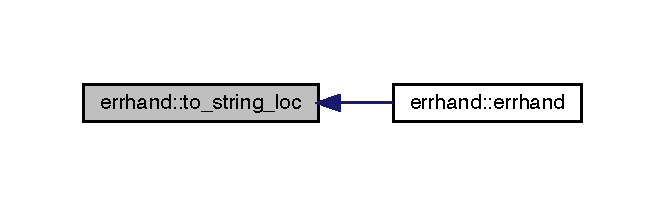
\includegraphics[width=319pt]{classerrhand_a930df1c197154853159683cb2ad55369_icgraph}
\end{center}
\end{figure}


\subsubsection{Member Data Documentation}
\mbox{\Hypertarget{classerrhand_a2baa975c76a80afce9c97575c549058c}\label{classerrhand_a2baa975c76a80afce9c97575c549058c}} 
\index{errhand@{errhand}!err\+\_\+msg@{err\+\_\+msg}}
\index{err\+\_\+msg@{err\+\_\+msg}!errhand@{errhand}}
\paragraph{\texorpdfstring{err\+\_\+msg}{err\_msg}}
{\footnotesize\ttfamily std\+::string errhand\+::err\+\_\+msg\hspace{0.3cm}{\ttfamily [private]}}

\mbox{\Hypertarget{classerrhand_aed73d7a312fae4b4387d8d2487277a74}\label{classerrhand_aed73d7a312fae4b4387d8d2487277a74}} 
\index{errhand@{errhand}!file@{file}}
\index{file@{file}!errhand@{errhand}}
\paragraph{\texorpdfstring{file}{file}}
{\footnotesize\ttfamily std\+::string errhand\+::file\hspace{0.3cm}{\ttfamily [private]}}

\mbox{\Hypertarget{classerrhand_a3ddc204c758b97e7d1550019e4513f3b}\label{classerrhand_a3ddc204c758b97e7d1550019e4513f3b}} 
\index{errhand@{errhand}!line@{line}}
\index{line@{line}!errhand@{errhand}}
\paragraph{\texorpdfstring{line}{line}}
{\footnotesize\ttfamily size\+\_\+t errhand\+::line\hspace{0.3cm}{\ttfamily [private]}}



The documentation for this class was generated from the following file\+:\begin{DoxyCompactItemize}
\item 
\mbox{\hyperlink{errhand_8h}{errhand.\+h}}\end{DoxyCompactItemize}

\hypertarget{class_g_a_r}{}\section{G\+AR$<$ Data\+Type, N $>$ Class Template Reference}
\label{class_g_a_r}\index{G\+A\+R$<$ Data\+Type, N $>$@{G\+A\+R$<$ Data\+Type, N $>$}}


Class of velocity dependent dynamical system with regularization variables.  




{\ttfamily \#include $<$G\+A\+R.\+h$>$}

\subsection*{Public Types}
\begin{DoxyCompactItemize}
\item 
typedef Data\+Type \mbox{\hyperlink{class_g_a_r_a2ae44eda8e28d5dd26cf707dcda69314}{Scalar}}
\item 
typedef \mbox{\hyperlink{structvec3}{vec3}}$<$ \mbox{\hyperlink{class_g_a_r_a2ae44eda8e28d5dd26cf707dcda69314}{Scalar}} $>$ \mbox{\hyperlink{class_g_a_r_ad2f5b930feb3831a717f96155b3ff74e}{Vector}}
\item 
typedef std\+::array$<$ \mbox{\hyperlink{structvec3}{vec3}}$<$ \mbox{\hyperlink{class_g_a_r_a2ae44eda8e28d5dd26cf707dcda69314}{Scalar}} $>$, N $>$ \mbox{\hyperlink{class_g_a_r_a5818e17eb203504af6e10f38fc38d378}{Vector\+Array}}
\item 
typedef std\+::array$<$ \mbox{\hyperlink{class_g_a_r_a2ae44eda8e28d5dd26cf707dcda69314}{Scalar}}, N $>$ \mbox{\hyperlink{class_g_a_r_a0b446684ae922457a3bf86c904085d8a}{Scalar\+Array}}
\item 
typedef std\+::array$<$ size\+\_\+t, N $>$ \mbox{\hyperlink{class_g_a_r_aaf033049c0cd8f0f86a82b9595086fa5}{Index\+Array}}
\end{DoxyCompactItemize}
\subsection*{Public Member Functions}
\begin{DoxyCompactItemize}
\item 
std\+::array$<$ \mbox{\hyperlink{class_g_a_r_a2ae44eda8e28d5dd26cf707dcda69314}{Scalar}}, \mbox{\hyperlink{class_g_a_r_abdbcc31db058125bd2ee207e7648b20b}{volume}}()$>$ \& \mbox{\hyperlink{class_g_a_r_a152aa5eea95fe568b010d85a7ba23bf7}{array}} ()
\begin{DoxyCompactList}\small\item\em Transfer this class to a plain array. \end{DoxyCompactList}\item 
void \mbox{\hyperlink{class_g_a_r_a3c59ee9bf8aae928644fa2beabbffa7c}{set\+Zero}} ()
\begin{DoxyCompactList}\small\item\em Set all data to be zero. \end{DoxyCompactList}\item 
\mbox{\hyperlink{class_g_a_r_a2ae44eda8e28d5dd26cf707dcda69314}{Scalar}} \mbox{\hyperlink{class_g_a_r_a3d5871f25d147497399fa65343bca84a}{get\+Omega}} (const \mbox{\hyperlink{class_g_a_r_a0b446684ae922457a3bf86c904085d8a}{Scalar\+Array}} \&mass)
\begin{DoxyCompactList}\small\item\em Calculate the regularization variable omega. \end{DoxyCompactList}\item 
void \mbox{\hyperlink{class_g_a_r_a31b5ad2527cc52d1422fa11e2d93fbc6}{init\+Addi\+Variable}} (\mbox{\hyperlink{class_g_a_r_a0b446684ae922457a3bf86c904085d8a}{Scalar\+Array}} \&mass)
\begin{DoxyCompactList}\small\item\em Initialize extra user defined variables. Interface required for other class. \end{DoxyCompactList}\item 
void \mbox{\hyperlink{class_g_a_r_a18041ac48dc47e6ada3e8a33893b1200}{to\+Chain}} (\mbox{\hyperlink{class_g_a_r}{G\+AR}} \&chain\+Data, \mbox{\hyperlink{class_g_a_r_aaf033049c0cd8f0f86a82b9595086fa5}{Index\+Array}} \&index)
\begin{DoxyCompactList}\small\item\em Transfer Cartesian coordinate regularization system to chain regularization system. \end{DoxyCompactList}\item 
void \mbox{\hyperlink{class_g_a_r_a2a282218e90ffb1a367da364b70e54a3}{to\+Cartesian}} (\mbox{\hyperlink{class_g_a_r}{G\+AR}} \&cartesian, \mbox{\hyperlink{class_g_a_r_aaf033049c0cd8f0f86a82b9595086fa5}{Index\+Array}} \&index)
\begin{DoxyCompactList}\small\item\em Transfer chain coordinate regularization system to Cartesian regularization system. \end{DoxyCompactList}\item 
void \mbox{\hyperlink{class_g_a_r_a373d938047a04b051683ee93198b1832}{move\+To\+Central\+Mass\+Coords}} (\mbox{\hyperlink{class_g_a_r_a0b446684ae922457a3bf86c904085d8a}{Scalar\+Array}} \&mass)
\begin{DoxyCompactList}\small\item\em Move particles to central mass coordinates. \end{DoxyCompactList}\end{DoxyCompactItemize}
\subsection*{Static Public Member Functions}
\begin{DoxyCompactItemize}
\item 
static constexpr size\+\_\+t \mbox{\hyperlink{class_g_a_r_a850c24cdfd1656389e3e42f575035edb}{size}} ()
\begin{DoxyCompactList}\small\item\em Get the number of the particles. \end{DoxyCompactList}\item 
static constexpr size\+\_\+t \mbox{\hyperlink{class_g_a_r_abdbcc31db058125bd2ee207e7648b20b}{volume}} ()
\begin{DoxyCompactList}\small\item\em Get the total data number. \end{DoxyCompactList}\end{DoxyCompactItemize}
\subsection*{Public Attributes}
\begin{DoxyCompactItemize}
\item 
\mbox{\hyperlink{class_g_a_r_a5818e17eb203504af6e10f38fc38d378}{Vector\+Array}} \mbox{\hyperlink{class_g_a_r_aec6b3fdb2c4dd7bdae27c0b41fbf6dda}{pos}}
\begin{DoxyCompactList}\small\item\em Array of position of the particles. Element is 3D vector. \end{DoxyCompactList}\item 
\mbox{\hyperlink{class_g_a_r_a5818e17eb203504af6e10f38fc38d378}{Vector\+Array}} \mbox{\hyperlink{class_g_a_r_a9619f6250eb37cb006bd508591f01997}{vel}}
\begin{DoxyCompactList}\small\item\em Array of velocity of the particles. Element is 3D vector. \end{DoxyCompactList}\item 
\mbox{\hyperlink{class_g_a_r_a5818e17eb203504af6e10f38fc38d378}{Vector\+Array}} \mbox{\hyperlink{class_g_a_r_ade7c1f936a5f23a0ded2d02b2cc750e6}{auxi\+Vel}}
\begin{DoxyCompactList}\small\item\em Array of auxiliary velocity of the particles. Element is 3D vector. \end{DoxyCompactList}\item 
\mbox{\hyperlink{class_g_a_r_a2ae44eda8e28d5dd26cf707dcda69314}{Scalar}} \mbox{\hyperlink{class_g_a_r_afaec5fb6242a3e5ae5cd368832cd1bb8}{time}} \{0.\+0\}
\begin{DoxyCompactList}\small\item\em The physical time of the dynamic system. \end{DoxyCompactList}\item 
\mbox{\hyperlink{class_g_a_r_a2ae44eda8e28d5dd26cf707dcda69314}{Scalar}} \mbox{\hyperlink{class_g_a_r_a10f49216d9cacb2b21bd053a2ddb997c}{bindE}} \{0.\+0\}
\begin{DoxyCompactList}\small\item\em The binding energy(for regularization) of the dynamic system. \end{DoxyCompactList}\item 
\mbox{\hyperlink{class_g_a_r_a2ae44eda8e28d5dd26cf707dcda69314}{Scalar}} \mbox{\hyperlink{class_g_a_r_a702f19b87d8754ac66914985d7c8229e}{omega}} \{0.\+0\}
\begin{DoxyCompactList}\small\item\em The regularization variable of the dynamic system. \end{DoxyCompactList}\end{DoxyCompactItemize}


\subsection{Detailed Description}
\subsubsection*{template$<$typename Data\+Type, size\+\_\+t N$>$\newline
class G\+A\+R$<$ Data\+Type, N $>$}

Class of velocity dependent dynamical system with regularization variables. 

A simple extension of class dynamics in \mbox{\hyperlink{dynamic_state_8h}{dynamic\+State.\+h}}. Used for regularization system. See detail in \href{https://academic.oup.com/mnras/article/372/1/219/974304}{\tt https\+://academic.\+oup.\+com/mnras/article/372/1/219/974304} . 

\subsection{Member Typedef Documentation}
\mbox{\Hypertarget{class_g_a_r_aaf033049c0cd8f0f86a82b9595086fa5}\label{class_g_a_r_aaf033049c0cd8f0f86a82b9595086fa5}} 
\index{G\+AR@{G\+AR}!Index\+Array@{Index\+Array}}
\index{Index\+Array@{Index\+Array}!G\+AR@{G\+AR}}
\subsubsection{\texorpdfstring{Index\+Array}{IndexArray}}
{\footnotesize\ttfamily template$<$typename Data\+Type , size\+\_\+t N$>$ \\
typedef std\+::array$<$size\+\_\+t, N$>$ \mbox{\hyperlink{class_g_a_r}{G\+AR}}$<$ Data\+Type, N $>$\+::\mbox{\hyperlink{class_g_a_r_aaf033049c0cd8f0f86a82b9595086fa5}{Index\+Array}}}

\mbox{\Hypertarget{class_g_a_r_a2ae44eda8e28d5dd26cf707dcda69314}\label{class_g_a_r_a2ae44eda8e28d5dd26cf707dcda69314}} 
\index{G\+AR@{G\+AR}!Scalar@{Scalar}}
\index{Scalar@{Scalar}!G\+AR@{G\+AR}}
\subsubsection{\texorpdfstring{Scalar}{Scalar}}
{\footnotesize\ttfamily template$<$typename Data\+Type , size\+\_\+t N$>$ \\
typedef Data\+Type \mbox{\hyperlink{class_g_a_r}{G\+AR}}$<$ Data\+Type, N $>$\+::\mbox{\hyperlink{class_g_a_r_a2ae44eda8e28d5dd26cf707dcda69314}{Scalar}}}

\mbox{\Hypertarget{class_g_a_r_a0b446684ae922457a3bf86c904085d8a}\label{class_g_a_r_a0b446684ae922457a3bf86c904085d8a}} 
\index{G\+AR@{G\+AR}!Scalar\+Array@{Scalar\+Array}}
\index{Scalar\+Array@{Scalar\+Array}!G\+AR@{G\+AR}}
\subsubsection{\texorpdfstring{Scalar\+Array}{ScalarArray}}
{\footnotesize\ttfamily template$<$typename Data\+Type , size\+\_\+t N$>$ \\
typedef std\+::array$<$\mbox{\hyperlink{class_g_a_r_a2ae44eda8e28d5dd26cf707dcda69314}{Scalar}}, N$>$ \mbox{\hyperlink{class_g_a_r}{G\+AR}}$<$ Data\+Type, N $>$\+::\mbox{\hyperlink{class_g_a_r_a0b446684ae922457a3bf86c904085d8a}{Scalar\+Array}}}

\mbox{\Hypertarget{class_g_a_r_ad2f5b930feb3831a717f96155b3ff74e}\label{class_g_a_r_ad2f5b930feb3831a717f96155b3ff74e}} 
\index{G\+AR@{G\+AR}!Vector@{Vector}}
\index{Vector@{Vector}!G\+AR@{G\+AR}}
\subsubsection{\texorpdfstring{Vector}{Vector}}
{\footnotesize\ttfamily template$<$typename Data\+Type , size\+\_\+t N$>$ \\
typedef \mbox{\hyperlink{structvec3}{vec3}}$<$\mbox{\hyperlink{class_g_a_r_a2ae44eda8e28d5dd26cf707dcda69314}{Scalar}}$>$ \mbox{\hyperlink{class_g_a_r}{G\+AR}}$<$ Data\+Type, N $>$\+::\mbox{\hyperlink{class_g_a_r_ad2f5b930feb3831a717f96155b3ff74e}{Vector}}}

\mbox{\Hypertarget{class_g_a_r_a5818e17eb203504af6e10f38fc38d378}\label{class_g_a_r_a5818e17eb203504af6e10f38fc38d378}} 
\index{G\+AR@{G\+AR}!Vector\+Array@{Vector\+Array}}
\index{Vector\+Array@{Vector\+Array}!G\+AR@{G\+AR}}
\subsubsection{\texorpdfstring{Vector\+Array}{VectorArray}}
{\footnotesize\ttfamily template$<$typename Data\+Type , size\+\_\+t N$>$ \\
typedef std\+::array$<$\mbox{\hyperlink{structvec3}{vec3}}$<$\mbox{\hyperlink{class_g_a_r_a2ae44eda8e28d5dd26cf707dcda69314}{Scalar}}$>$, N$>$ \mbox{\hyperlink{class_g_a_r}{G\+AR}}$<$ Data\+Type, N $>$\+::\mbox{\hyperlink{class_g_a_r_a5818e17eb203504af6e10f38fc38d378}{Vector\+Array}}}



\subsection{Member Function Documentation}
\mbox{\Hypertarget{class_g_a_r_a152aa5eea95fe568b010d85a7ba23bf7}\label{class_g_a_r_a152aa5eea95fe568b010d85a7ba23bf7}} 
\index{G\+AR@{G\+AR}!array@{array}}
\index{array@{array}!G\+AR@{G\+AR}}
\subsubsection{\texorpdfstring{array()}{array()}}
{\footnotesize\ttfamily template$<$typename Data\+Type , size\+\_\+t N$>$ \\
std\+::array$<$\mbox{\hyperlink{class_g_a_r_a2ae44eda8e28d5dd26cf707dcda69314}{Scalar}}, \mbox{\hyperlink{class_g_a_r_abdbcc31db058125bd2ee207e7648b20b}{volume}}()$>$\& \mbox{\hyperlink{class_g_a_r}{G\+AR}}$<$ Data\+Type, N $>$\+::array (\begin{DoxyParamCaption}{ }\end{DoxyParamCaption})\hspace{0.3cm}{\ttfamily [inline]}}



Transfer this class to a plain array. 

\begin{DoxyReturn}{Returns}
The reference of head of this class, reinterpret as a plain array. 
\end{DoxyReturn}
\mbox{\Hypertarget{class_g_a_r_a3d5871f25d147497399fa65343bca84a}\label{class_g_a_r_a3d5871f25d147497399fa65343bca84a}} 
\index{G\+AR@{G\+AR}!get\+Omega@{get\+Omega}}
\index{get\+Omega@{get\+Omega}!G\+AR@{G\+AR}}
\subsubsection{\texorpdfstring{get\+Omega()}{getOmega()}}
{\footnotesize\ttfamily template$<$typename Data\+Type , size\+\_\+t N$>$ \\
\mbox{\hyperlink{class_g_a_r_a2ae44eda8e28d5dd26cf707dcda69314}{Scalar}} \mbox{\hyperlink{class_g_a_r}{G\+AR}}$<$ Data\+Type, N $>$\+::get\+Omega (\begin{DoxyParamCaption}\item[{const \mbox{\hyperlink{class_g_a_r_a0b446684ae922457a3bf86c904085d8a}{Scalar\+Array}} \&}]{mass }\end{DoxyParamCaption})\hspace{0.3cm}{\ttfamily [inline]}}



Calculate the regularization variable omega. 


\begin{DoxyParams}{Parameters}
{\em mass} & The mass of particles, might be required for calculation. \\
\hline
\end{DoxyParams}
\begin{DoxyReturn}{Returns}
The calculated value of omega. 
\end{DoxyReturn}
Here is the call graph for this function\+:\nopagebreak
\begin{figure}[H]
\begin{center}
\leavevmode
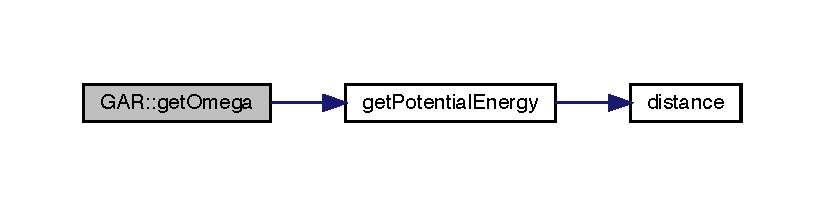
\includegraphics[width=350pt]{class_g_a_r_a3d5871f25d147497399fa65343bca84a_cgraph}
\end{center}
\end{figure}
Here is the caller graph for this function\+:\nopagebreak
\begin{figure}[H]
\begin{center}
\leavevmode
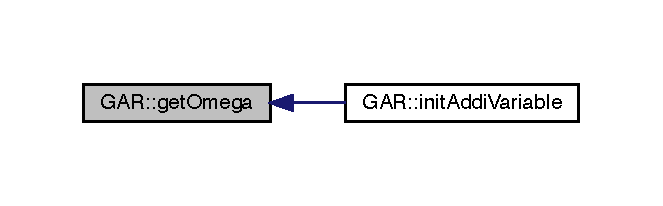
\includegraphics[width=318pt]{class_g_a_r_a3d5871f25d147497399fa65343bca84a_icgraph}
\end{center}
\end{figure}
\mbox{\Hypertarget{class_g_a_r_a31b5ad2527cc52d1422fa11e2d93fbc6}\label{class_g_a_r_a31b5ad2527cc52d1422fa11e2d93fbc6}} 
\index{G\+AR@{G\+AR}!init\+Addi\+Variable@{init\+Addi\+Variable}}
\index{init\+Addi\+Variable@{init\+Addi\+Variable}!G\+AR@{G\+AR}}
\subsubsection{\texorpdfstring{init\+Addi\+Variable()}{initAddiVariable()}}
{\footnotesize\ttfamily template$<$typename Data\+Type , size\+\_\+t N$>$ \\
void \mbox{\hyperlink{class_g_a_r}{G\+AR}}$<$ Data\+Type, N $>$\+::init\+Addi\+Variable (\begin{DoxyParamCaption}\item[{\mbox{\hyperlink{class_g_a_r_a0b446684ae922457a3bf86c904085d8a}{Scalar\+Array}} \&}]{mass }\end{DoxyParamCaption})\hspace{0.3cm}{\ttfamily [inline]}}



Initialize extra user defined variables. Interface required for other class. 

Initialize regularizaiton variable bindE and omega. 
\begin{DoxyParams}{Parameters}
{\em mass} & The mass of particles, might be required for initialization. \\
\hline
\end{DoxyParams}
Here is the call graph for this function\+:\nopagebreak
\begin{figure}[H]
\begin{center}
\leavevmode
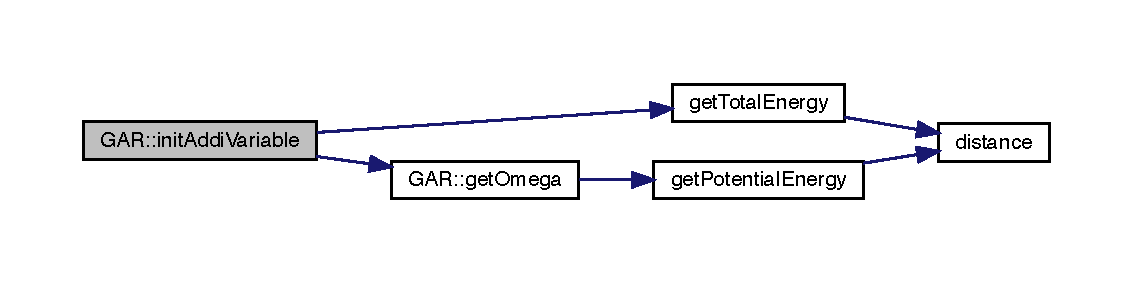
\includegraphics[width=350pt]{class_g_a_r_a31b5ad2527cc52d1422fa11e2d93fbc6_cgraph}
\end{center}
\end{figure}
\mbox{\Hypertarget{class_g_a_r_a373d938047a04b051683ee93198b1832}\label{class_g_a_r_a373d938047a04b051683ee93198b1832}} 
\index{G\+AR@{G\+AR}!move\+To\+Central\+Mass\+Coords@{move\+To\+Central\+Mass\+Coords}}
\index{move\+To\+Central\+Mass\+Coords@{move\+To\+Central\+Mass\+Coords}!G\+AR@{G\+AR}}
\subsubsection{\texorpdfstring{move\+To\+Central\+Mass\+Coords()}{moveToCentralMassCoords()}}
{\footnotesize\ttfamily template$<$typename Data\+Type , size\+\_\+t N$>$ \\
void \mbox{\hyperlink{class_g_a_r}{G\+AR}}$<$ Data\+Type, N $>$\+::move\+To\+Central\+Mass\+Coords (\begin{DoxyParamCaption}\item[{\mbox{\hyperlink{class_g_a_r_a0b446684ae922457a3bf86c904085d8a}{Scalar\+Array}} \&}]{mass }\end{DoxyParamCaption})\hspace{0.3cm}{\ttfamily [inline]}}



Move particles to central mass coordinates. 

Move position, velocity and auxiliary velocity to central mass coordinates. 
\begin{DoxyParams}{Parameters}
{\em mass} & Mass of the particles required for moving. \\
\hline
\end{DoxyParams}
Here is the call graph for this function\+:\nopagebreak
\begin{figure}[H]
\begin{center}
\leavevmode
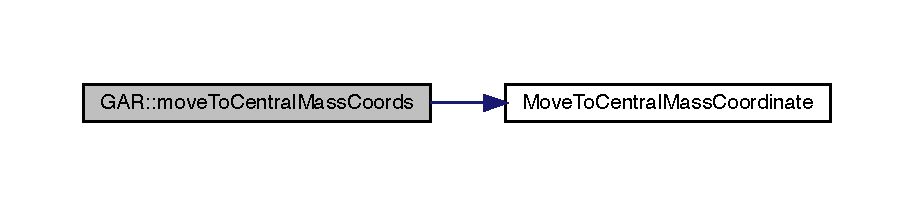
\includegraphics[width=350pt]{class_g_a_r_a373d938047a04b051683ee93198b1832_cgraph}
\end{center}
\end{figure}
\mbox{\Hypertarget{class_g_a_r_a3c59ee9bf8aae928644fa2beabbffa7c}\label{class_g_a_r_a3c59ee9bf8aae928644fa2beabbffa7c}} 
\index{G\+AR@{G\+AR}!set\+Zero@{set\+Zero}}
\index{set\+Zero@{set\+Zero}!G\+AR@{G\+AR}}
\subsubsection{\texorpdfstring{set\+Zero()}{setZero()}}
{\footnotesize\ttfamily template$<$typename Data\+Type , size\+\_\+t N$>$ \\
void \mbox{\hyperlink{class_g_a_r}{G\+AR}}$<$ Data\+Type, N $>$\+::set\+Zero (\begin{DoxyParamCaption}{ }\end{DoxyParamCaption})\hspace{0.3cm}{\ttfamily [inline]}}



Set all data to be zero. 

Here is the call graph for this function\+:\nopagebreak
\begin{figure}[H]
\begin{center}
\leavevmode
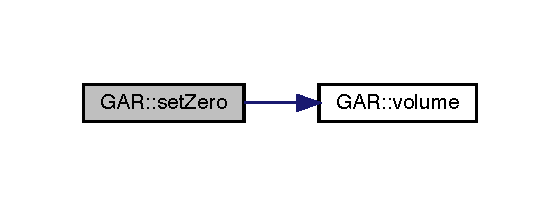
\includegraphics[width=269pt]{class_g_a_r_a3c59ee9bf8aae928644fa2beabbffa7c_cgraph}
\end{center}
\end{figure}
\mbox{\Hypertarget{class_g_a_r_a850c24cdfd1656389e3e42f575035edb}\label{class_g_a_r_a850c24cdfd1656389e3e42f575035edb}} 
\index{G\+AR@{G\+AR}!size@{size}}
\index{size@{size}!G\+AR@{G\+AR}}
\subsubsection{\texorpdfstring{size()}{size()}}
{\footnotesize\ttfamily template$<$typename Data\+Type , size\+\_\+t N$>$ \\
static constexpr size\+\_\+t \mbox{\hyperlink{class_g_a_r}{G\+AR}}$<$ Data\+Type, N $>$\+::size (\begin{DoxyParamCaption}{ }\end{DoxyParamCaption})\hspace{0.3cm}{\ttfamily [inline]}, {\ttfamily [static]}}



Get the number of the particles. 

\begin{DoxyReturn}{Returns}
The particle number. 
\end{DoxyReturn}
\mbox{\Hypertarget{class_g_a_r_a2a282218e90ffb1a367da364b70e54a3}\label{class_g_a_r_a2a282218e90ffb1a367da364b70e54a3}} 
\index{G\+AR@{G\+AR}!to\+Cartesian@{to\+Cartesian}}
\index{to\+Cartesian@{to\+Cartesian}!G\+AR@{G\+AR}}
\subsubsection{\texorpdfstring{to\+Cartesian()}{toCartesian()}}
{\footnotesize\ttfamily template$<$typename Data\+Type , size\+\_\+t N$>$ \\
void \mbox{\hyperlink{class_g_a_r}{G\+AR}}$<$ Data\+Type, N $>$\+::to\+Cartesian (\begin{DoxyParamCaption}\item[{\mbox{\hyperlink{class_g_a_r}{G\+AR}}$<$ Data\+Type, N $>$ \&}]{cartesian,  }\item[{\mbox{\hyperlink{class_g_a_r_aaf033049c0cd8f0f86a82b9595086fa5}{Index\+Array}} \&}]{index }\end{DoxyParamCaption})\hspace{0.3cm}{\ttfamily [inline]}}



Transfer chain coordinate regularization system to Cartesian regularization system. 

Coordinate transformation. From chain to Cartesian. See details in \href{https://link.springer.com/article/10.1007%2FBF00695714}{\tt https\+://link.\+springer.\+com/article/10.\+1007\%2\+F\+B\+F00695714} . 
\begin{DoxyParams}{Parameters}
{\em cartesian} & The destination regularization system in Cartesian coordinates. \\
\hline
{\em index} & The maping index between Cartesian coordinates and chain coordinates. \\
\hline
\end{DoxyParams}
Here is the call graph for this function\+:\nopagebreak
\begin{figure}[H]
\begin{center}
\leavevmode
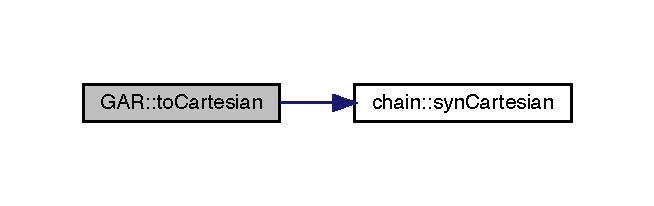
\includegraphics[width=314pt]{class_g_a_r_a2a282218e90ffb1a367da364b70e54a3_cgraph}
\end{center}
\end{figure}
\mbox{\Hypertarget{class_g_a_r_a18041ac48dc47e6ada3e8a33893b1200}\label{class_g_a_r_a18041ac48dc47e6ada3e8a33893b1200}} 
\index{G\+AR@{G\+AR}!to\+Chain@{to\+Chain}}
\index{to\+Chain@{to\+Chain}!G\+AR@{G\+AR}}
\subsubsection{\texorpdfstring{to\+Chain()}{toChain()}}
{\footnotesize\ttfamily template$<$typename Data\+Type , size\+\_\+t N$>$ \\
void \mbox{\hyperlink{class_g_a_r}{G\+AR}}$<$ Data\+Type, N $>$\+::to\+Chain (\begin{DoxyParamCaption}\item[{\mbox{\hyperlink{class_g_a_r}{G\+AR}}$<$ Data\+Type, N $>$ \&}]{chain\+Data,  }\item[{\mbox{\hyperlink{class_g_a_r_aaf033049c0cd8f0f86a82b9595086fa5}{Index\+Array}} \&}]{index }\end{DoxyParamCaption})\hspace{0.3cm}{\ttfamily [inline]}}



Transfer Cartesian coordinate regularization system to chain regularization system. 

Coordinate transformation. From Cartesian to chain. See details in \href{https://link.springer.com/article/10.1007%2FBF00695714}{\tt https\+://link.\+springer.\+com/article/10.\+1007\%2\+F\+B\+F00695714} . 
\begin{DoxyParams}{Parameters}
{\em chain\+Data} & The destination regularization system in chain coordinates. \\
\hline
{\em index} & The maping index between Cartesian coordinates and chain coordinates. \\
\hline
\end{DoxyParams}
Here is the call graph for this function\+:\nopagebreak
\begin{figure}[H]
\begin{center}
\leavevmode
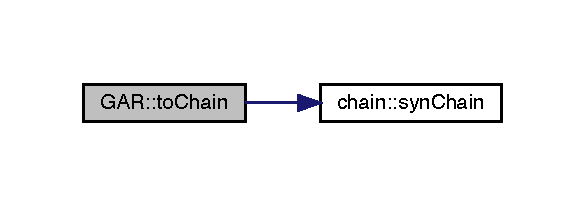
\includegraphics[width=281pt]{class_g_a_r_a18041ac48dc47e6ada3e8a33893b1200_cgraph}
\end{center}
\end{figure}
\mbox{\Hypertarget{class_g_a_r_abdbcc31db058125bd2ee207e7648b20b}\label{class_g_a_r_abdbcc31db058125bd2ee207e7648b20b}} 
\index{G\+AR@{G\+AR}!volume@{volume}}
\index{volume@{volume}!G\+AR@{G\+AR}}
\subsubsection{\texorpdfstring{volume()}{volume()}}
{\footnotesize\ttfamily template$<$typename Data\+Type , size\+\_\+t N$>$ \\
static constexpr size\+\_\+t \mbox{\hyperlink{class_g_a_r}{G\+AR}}$<$ Data\+Type, N $>$\+::volume (\begin{DoxyParamCaption}{ }\end{DoxyParamCaption})\hspace{0.3cm}{\ttfamily [inline]}, {\ttfamily [static]}}



Get the total data number. 

\begin{DoxyReturn}{Returns}
The data number. 
\end{DoxyReturn}
Here is the caller graph for this function\+:\nopagebreak
\begin{figure}[H]
\begin{center}
\leavevmode
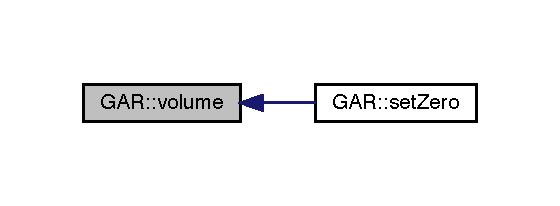
\includegraphics[width=269pt]{class_g_a_r_abdbcc31db058125bd2ee207e7648b20b_icgraph}
\end{center}
\end{figure}


\subsection{Member Data Documentation}
\mbox{\Hypertarget{class_g_a_r_ade7c1f936a5f23a0ded2d02b2cc750e6}\label{class_g_a_r_ade7c1f936a5f23a0ded2d02b2cc750e6}} 
\index{G\+AR@{G\+AR}!auxi\+Vel@{auxi\+Vel}}
\index{auxi\+Vel@{auxi\+Vel}!G\+AR@{G\+AR}}
\subsubsection{\texorpdfstring{auxi\+Vel}{auxiVel}}
{\footnotesize\ttfamily template$<$typename Data\+Type , size\+\_\+t N$>$ \\
\mbox{\hyperlink{class_g_a_r_a5818e17eb203504af6e10f38fc38d378}{Vector\+Array}} \mbox{\hyperlink{class_g_a_r}{G\+AR}}$<$ Data\+Type, N $>$\+::auxi\+Vel}



Array of auxiliary velocity of the particles. Element is 3D vector. 

\mbox{\Hypertarget{class_g_a_r_a10f49216d9cacb2b21bd053a2ddb997c}\label{class_g_a_r_a10f49216d9cacb2b21bd053a2ddb997c}} 
\index{G\+AR@{G\+AR}!bindE@{bindE}}
\index{bindE@{bindE}!G\+AR@{G\+AR}}
\subsubsection{\texorpdfstring{bindE}{bindE}}
{\footnotesize\ttfamily template$<$typename Data\+Type , size\+\_\+t N$>$ \\
\mbox{\hyperlink{class_g_a_r_a2ae44eda8e28d5dd26cf707dcda69314}{Scalar}} \mbox{\hyperlink{class_g_a_r}{G\+AR}}$<$ Data\+Type, N $>$\+::bindE \{0.\+0\}}



The binding energy(for regularization) of the dynamic system. 

\mbox{\Hypertarget{class_g_a_r_a702f19b87d8754ac66914985d7c8229e}\label{class_g_a_r_a702f19b87d8754ac66914985d7c8229e}} 
\index{G\+AR@{G\+AR}!omega@{omega}}
\index{omega@{omega}!G\+AR@{G\+AR}}
\subsubsection{\texorpdfstring{omega}{omega}}
{\footnotesize\ttfamily template$<$typename Data\+Type , size\+\_\+t N$>$ \\
\mbox{\hyperlink{class_g_a_r_a2ae44eda8e28d5dd26cf707dcda69314}{Scalar}} \mbox{\hyperlink{class_g_a_r}{G\+AR}}$<$ Data\+Type, N $>$\+::omega \{0.\+0\}}



The regularization variable of the dynamic system. 

\mbox{\Hypertarget{class_g_a_r_aec6b3fdb2c4dd7bdae27c0b41fbf6dda}\label{class_g_a_r_aec6b3fdb2c4dd7bdae27c0b41fbf6dda}} 
\index{G\+AR@{G\+AR}!pos@{pos}}
\index{pos@{pos}!G\+AR@{G\+AR}}
\subsubsection{\texorpdfstring{pos}{pos}}
{\footnotesize\ttfamily template$<$typename Data\+Type , size\+\_\+t N$>$ \\
\mbox{\hyperlink{class_g_a_r_a5818e17eb203504af6e10f38fc38d378}{Vector\+Array}} \mbox{\hyperlink{class_g_a_r}{G\+AR}}$<$ Data\+Type, N $>$\+::pos}



Array of position of the particles. Element is 3D vector. 

\mbox{\Hypertarget{class_g_a_r_afaec5fb6242a3e5ae5cd368832cd1bb8}\label{class_g_a_r_afaec5fb6242a3e5ae5cd368832cd1bb8}} 
\index{G\+AR@{G\+AR}!time@{time}}
\index{time@{time}!G\+AR@{G\+AR}}
\subsubsection{\texorpdfstring{time}{time}}
{\footnotesize\ttfamily template$<$typename Data\+Type , size\+\_\+t N$>$ \\
\mbox{\hyperlink{class_g_a_r_a2ae44eda8e28d5dd26cf707dcda69314}{Scalar}} \mbox{\hyperlink{class_g_a_r}{G\+AR}}$<$ Data\+Type, N $>$\+::time \{0.\+0\}}



The physical time of the dynamic system. 

\mbox{\Hypertarget{class_g_a_r_a9619f6250eb37cb006bd508591f01997}\label{class_g_a_r_a9619f6250eb37cb006bd508591f01997}} 
\index{G\+AR@{G\+AR}!vel@{vel}}
\index{vel@{vel}!G\+AR@{G\+AR}}
\subsubsection{\texorpdfstring{vel}{vel}}
{\footnotesize\ttfamily template$<$typename Data\+Type , size\+\_\+t N$>$ \\
\mbox{\hyperlink{class_g_a_r_a5818e17eb203504af6e10f38fc38d378}{Vector\+Array}} \mbox{\hyperlink{class_g_a_r}{G\+AR}}$<$ Data\+Type, N $>$\+::vel}



Array of velocity of the particles. Element is 3D vector. 



The documentation for this class was generated from the following file\+:\begin{DoxyCompactItemize}
\item 
particle\+System/\mbox{\hyperlink{_g_a_r_8h}{G\+A\+R.\+h}}\end{DoxyCompactItemize}

\hypertarget{classlog_h}{}\subsection{logH$<$ Dynamic\+State $>$ Class Template Reference}
\label{classlog_h}\index{log\+H$<$ Dynamic\+State $>$@{log\+H$<$ Dynamic\+State $>$}}


\mbox{\hyperlink{classlog_h}{logH}} extention algorithmatic regularization interface  




{\ttfamily \#include $<$regularization.\+h$>$}

\subsubsection*{Public Types}
\begin{DoxyCompactItemize}
\item 
typedef Dynamic\+State\+::\+Scalar \mbox{\hyperlink{classlog_h_a3c5a69c2908971aa6cd8ff82845418d0}{Scalar}}
\end{DoxyCompactItemize}
\subsubsection*{Public Member Functions}
\begin{DoxyCompactItemize}
\item 
\mbox{\hyperlink{classlog_h_a3c5a69c2908971aa6cd8ff82845418d0}{Scalar}} \mbox{\hyperlink{classlog_h_a57fa85fad38dae198ec4eadd757d4f40}{get\+Physical\+Pos\+Time}} (std\+::array$<$ \mbox{\hyperlink{classlog_h_a3c5a69c2908971aa6cd8ff82845418d0}{Scalar}}, \mbox{\hyperlink{classlog_h_a94f9577ea2cc32d422ebf078e123480b}{size}}()$>$ \&mass, Dynamic\+State \&dyn, \mbox{\hyperlink{classlog_h_a3c5a69c2908971aa6cd8ff82845418d0}{Scalar}} step\+Size)
\begin{DoxyCompactList}\small\item\em Calculate the physical time for position advance from integration step size. \end{DoxyCompactList}\item 
\mbox{\hyperlink{classlog_h_a3c5a69c2908971aa6cd8ff82845418d0}{Scalar}} \mbox{\hyperlink{classlog_h_a4e287cd21c48b51fa9535c5b692ca3f2}{get\+Physical\+Vel\+Time}} (std\+::array$<$ \mbox{\hyperlink{classlog_h_a3c5a69c2908971aa6cd8ff82845418d0}{Scalar}}, \mbox{\hyperlink{classlog_h_a94f9577ea2cc32d422ebf078e123480b}{size}}()$>$ \&mass, Dynamic\+State \&dyn, \mbox{\hyperlink{classlog_h_a3c5a69c2908971aa6cd8ff82845418d0}{Scalar}} step\+Size)
\begin{DoxyCompactList}\small\item\em Calculate the physical time for velocity advance from integration step size. \end{DoxyCompactList}\end{DoxyCompactItemize}
\subsubsection*{Static Public Member Functions}
\begin{DoxyCompactItemize}
\item 
static constexpr size\+\_\+t \mbox{\hyperlink{classlog_h_a94f9577ea2cc32d422ebf078e123480b}{size}} ()
\end{DoxyCompactItemize}


\subsubsection{Detailed Description}
\subsubsection*{template$<$typename Dynamic\+State$>$\newline
class log\+H$<$ Dynamic\+State $>$}

\mbox{\hyperlink{classlog_h}{logH}} extention algorithmatic regularization interface 

See detials in \href{https://link.springer.com/article/10.1023%2FA%3A1008368322547}{\tt https\+://link.\+springer.\+com/article/10.\+1023\%2\+F\+A\%3\+A1008368322547} and \href{http://iopscience.iop.org/article/10.1086/301102/meta}{\tt http\+://iopscience.\+iop.\+org/article/10.\+1086/301102/meta} . 

\subsubsection{Member Typedef Documentation}
\mbox{\Hypertarget{classlog_h_a3c5a69c2908971aa6cd8ff82845418d0}\label{classlog_h_a3c5a69c2908971aa6cd8ff82845418d0}} 
\index{logH@{logH}!Scalar@{Scalar}}
\index{Scalar@{Scalar}!logH@{logH}}
\paragraph{\texorpdfstring{Scalar}{Scalar}}
{\footnotesize\ttfamily template$<$typename Dynamic\+State $>$ \\
typedef Dynamic\+State\+::\+Scalar \mbox{\hyperlink{classlog_h}{logH}}$<$ Dynamic\+State $>$\+::\mbox{\hyperlink{classlog_h_a3c5a69c2908971aa6cd8ff82845418d0}{Scalar}}}



\subsubsection{Member Function Documentation}
\mbox{\Hypertarget{classlog_h_a57fa85fad38dae198ec4eadd757d4f40}\label{classlog_h_a57fa85fad38dae198ec4eadd757d4f40}} 
\index{logH@{logH}!get\+Physical\+Pos\+Time@{get\+Physical\+Pos\+Time}}
\index{get\+Physical\+Pos\+Time@{get\+Physical\+Pos\+Time}!logH@{logH}}
\paragraph{\texorpdfstring{get\+Physical\+Pos\+Time()}{getPhysicalPosTime()}}
{\footnotesize\ttfamily template$<$typename Dynamic\+State $>$ \\
\mbox{\hyperlink{classlog_h_a3c5a69c2908971aa6cd8ff82845418d0}{Scalar}} \mbox{\hyperlink{classlog_h}{logH}}$<$ Dynamic\+State $>$\+::get\+Physical\+Pos\+Time (\begin{DoxyParamCaption}\item[{std\+::array$<$ \mbox{\hyperlink{classlog_h_a3c5a69c2908971aa6cd8ff82845418d0}{Scalar}}, \mbox{\hyperlink{classlog_h_a94f9577ea2cc32d422ebf078e123480b}{size}}()$>$ \&}]{mass,  }\item[{Dynamic\+State \&}]{dyn,  }\item[{\mbox{\hyperlink{classlog_h_a3c5a69c2908971aa6cd8ff82845418d0}{Scalar}}}]{step\+Size }\end{DoxyParamCaption})\hspace{0.3cm}{\ttfamily [inline]}}



Calculate the physical time for position advance from integration step size. 


\begin{DoxyParams}{Parameters}
{\em mass} & Array of particle mass. \\
\hline
{\em dyn} & Dynamic system contains position, velocity and regularization variables. See example class in \mbox{\hyperlink{dynamic_state_8h}{dynamic\+State.\+h}}. \\
\hline
{\em step\+Size} & Integration step size. This could not be the physical time. Look references for details in class despriction. \\
\hline
\end{DoxyParams}
Here is the call graph for this function\+:\nopagebreak
\begin{figure}[H]
\begin{center}
\leavevmode
\includegraphics[width=340pt]{classlog_h_a57fa85fad38dae198ec4eadd757d4f40_cgraph}
\end{center}
\end{figure}
\mbox{\Hypertarget{classlog_h_a4e287cd21c48b51fa9535c5b692ca3f2}\label{classlog_h_a4e287cd21c48b51fa9535c5b692ca3f2}} 
\index{logH@{logH}!get\+Physical\+Vel\+Time@{get\+Physical\+Vel\+Time}}
\index{get\+Physical\+Vel\+Time@{get\+Physical\+Vel\+Time}!logH@{logH}}
\paragraph{\texorpdfstring{get\+Physical\+Vel\+Time()}{getPhysicalVelTime()}}
{\footnotesize\ttfamily template$<$typename Dynamic\+State $>$ \\
\mbox{\hyperlink{classlog_h_a3c5a69c2908971aa6cd8ff82845418d0}{Scalar}} \mbox{\hyperlink{classlog_h}{logH}}$<$ Dynamic\+State $>$\+::get\+Physical\+Vel\+Time (\begin{DoxyParamCaption}\item[{std\+::array$<$ \mbox{\hyperlink{classlog_h_a3c5a69c2908971aa6cd8ff82845418d0}{Scalar}}, \mbox{\hyperlink{classlog_h_a94f9577ea2cc32d422ebf078e123480b}{size}}()$>$ \&}]{mass,  }\item[{Dynamic\+State \&}]{dyn,  }\item[{\mbox{\hyperlink{classlog_h_a3c5a69c2908971aa6cd8ff82845418d0}{Scalar}}}]{step\+Size }\end{DoxyParamCaption})\hspace{0.3cm}{\ttfamily [inline]}}



Calculate the physical time for velocity advance from integration step size. 


\begin{DoxyParams}{Parameters}
{\em mass} & Array of particle mass. \\
\hline
{\em dyn} & Dynamic system contains position, velocity and regularization variables. See example class in \mbox{\hyperlink{dynamic_state_8h}{dynamic\+State.\+h}}. \\
\hline
{\em step\+Size} & Integration step size. This could not be the physical time. Look references for details in class despriction. \\
\hline
\end{DoxyParams}
Here is the call graph for this function\+:\nopagebreak
\begin{figure}[H]
\begin{center}
\leavevmode
\includegraphics[width=350pt]{classlog_h_a4e287cd21c48b51fa9535c5b692ca3f2_cgraph}
\end{center}
\end{figure}
\mbox{\Hypertarget{classlog_h_a94f9577ea2cc32d422ebf078e123480b}\label{classlog_h_a94f9577ea2cc32d422ebf078e123480b}} 
\index{logH@{logH}!size@{size}}
\index{size@{size}!logH@{logH}}
\paragraph{\texorpdfstring{size()}{size()}}
{\footnotesize\ttfamily template$<$typename Dynamic\+State $>$ \\
static constexpr size\+\_\+t \mbox{\hyperlink{classlog_h}{logH}}$<$ Dynamic\+State $>$\+::size (\begin{DoxyParamCaption}{ }\end{DoxyParamCaption})\hspace{0.3cm}{\ttfamily [inline]}, {\ttfamily [static]}}



The documentation for this class was generated from the following file\+:\begin{DoxyCompactItemize}
\item 
particle\+System/\mbox{\hyperlink{regularization_8h}{regularization.\+h}}\end{DoxyCompactItemize}

\hypertarget{class_newtonian}{}\subsection{Newtonian$<$ Scalar $>$ Class Template Reference}
\label{class_newtonian}\index{Newtonian$<$ Scalar $>$@{Newtonian$<$ Scalar $>$}}


Marker of None velocity dependent force functor(c++ std11)  




{\ttfamily \#include $<$interaction.\+h$>$}

\subsubsection*{Public Member Functions}
\begin{DoxyCompactItemize}
\item 
void \mbox{\hyperlink{class_newtonian_a13f6ce2d08ba777301542e001eab5f9b}{operator()}} ()
\end{DoxyCompactItemize}


\subsubsection{Detailed Description}
\subsubsection*{template$<$typename Scalar$>$\newline
class Newtonian$<$ Scalar $>$}

Marker of None velocity dependent force functor(c++ std11) 

\subsubsection{Member Function Documentation}
\mbox{\Hypertarget{class_newtonian_a13f6ce2d08ba777301542e001eab5f9b}\label{class_newtonian_a13f6ce2d08ba777301542e001eab5f9b}} 
\index{Newtonian@{Newtonian}!operator()@{operator()}}
\index{operator()@{operator()}!Newtonian@{Newtonian}}
\paragraph{\texorpdfstring{operator()()}{operator()()}}
{\footnotesize\ttfamily template$<$typename Scalar $>$ \\
void \mbox{\hyperlink{class_newtonian}{Newtonian}}$<$ Scalar $>$\+::operator() (\begin{DoxyParamCaption}{ }\end{DoxyParamCaption})\hspace{0.3cm}{\ttfamily [inline]}}



The documentation for this class was generated from the following file\+:\begin{DoxyCompactItemize}
\item 
interaction/\mbox{\hyperlink{interaction_8h}{interaction.\+h}}\end{DoxyCompactItemize}

\hypertarget{structchain_1_1_node}{}\subsection{chain_\+:\+:Node$<$ Scalar $>$ Struct Template Reference}
\label{structchain_1_1_node}\index{chain_\+::\+Node$<$ Scalar $>$@{chain_\+::\+Node$<$ Scalar $>$}}


Struture to store the relative distance and index of two particles.  




{\ttfamily \#include $<$chain_.\+h$>$}

\subsubsection*{Public Attributes}
\begin{DoxyCompactItemize}
\item 
Scalar \mbox{\hyperlink{structchain_1_1_node_a3a9ca49370eba9c8ce1d6b2a146c93ee}{Rij}}
\item 
size\+\_\+t \mbox{\hyperlink{structchain_1_1_node_a289ef3bad054158a446e53481c2a9d17}{i}}
\item 
size\+\_\+t \mbox{\hyperlink{structchain_1_1_node_aa41c0c59d6cdd4263a72b9e5284aa3d9}{j}}
\item 
bool \mbox{\hyperlink{structchain_1_1_node_ac06192f15a8dba90e35c508b17aa0e63}{available}}
\end{DoxyCompactItemize}


\subsubsection{Detailed Description}
\subsubsection*{template$<$typename Scalar$>$\newline
struct chain_\+::\+Node$<$ Scalar $>$}

Struture to store the relative distance and index of two particles. 

\subsubsection{Member Data Documentation}
\mbox{\Hypertarget{structchain_1_1_node_ac06192f15a8dba90e35c508b17aa0e63}\label{structchain_1_1_node_ac06192f15a8dba90e35c508b17aa0e63}} 
\index{chain_\+::\+Node@{chain_\+::\+Node}!available@{available}}
\index{available@{available}!chain_\+::\+Node@{chain_\+::\+Node}}
\paragraph{\texorpdfstring{available}{available}}
{\footnotesize\ttfamily template$<$typename Scalar$>$ \\
bool \mbox{\hyperlink{structchain_1_1_node}{chain_\+::\+Node}}$<$ Scalar $>$\+::available}

State of node. If this node can be chained. \mbox{\Hypertarget{structchain_1_1_node_a289ef3bad054158a446e53481c2a9d17}\label{structchain_1_1_node_a289ef3bad054158a446e53481c2a9d17}} 
\index{chain_\+::\+Node@{chain_\+::\+Node}!i@{i}}
\index{i@{i}!chain_\+::\+Node@{chain_\+::\+Node}}
\paragraph{\texorpdfstring{i}{i}}
{\footnotesize\ttfamily template$<$typename Scalar$>$ \\
size\+\_\+t \mbox{\hyperlink{structchain_1_1_node}{chain_\+::\+Node}}$<$ Scalar $>$\+::i}

Particle index. \mbox{\Hypertarget{structchain_1_1_node_aa41c0c59d6cdd4263a72b9e5284aa3d9}\label{structchain_1_1_node_aa41c0c59d6cdd4263a72b9e5284aa3d9}} 
\index{chain_\+::\+Node@{chain_\+::\+Node}!j@{j}}
\index{j@{j}!chain_\+::\+Node@{chain_\+::\+Node}}
\paragraph{\texorpdfstring{j}{j}}
{\footnotesize\ttfamily template$<$typename Scalar$>$ \\
size\+\_\+t \mbox{\hyperlink{structchain_1_1_node}{chain_\+::\+Node}}$<$ Scalar $>$\+::j}

Particle index. \mbox{\Hypertarget{structchain_1_1_node_a3a9ca49370eba9c8ce1d6b2a146c93ee}\label{structchain_1_1_node_a3a9ca49370eba9c8ce1d6b2a146c93ee}} 
\index{chain_\+::\+Node@{chain_\+::\+Node}!Rij@{Rij}}
\index{Rij@{Rij}!chain_\+::\+Node@{chain_\+::\+Node}}
\paragraph{\texorpdfstring{Rij}{Rij}}
{\footnotesize\ttfamily template$<$typename Scalar$>$ \\
Scalar \mbox{\hyperlink{structchain_1_1_node}{chain_\+::\+Node}}$<$ Scalar $>$\+::Rij}

Relative distance of two particles. 

The documentation for this struct was generated from the following file\+:\begin{DoxyCompactItemize}
\item 
particle\+System/\mbox{\hyperlink{chain_8h}{chain_.\+h}}\end{DoxyCompactItemize}

\hypertarget{class_no_regu}{}\section{No\+Regu$<$ Particles $>$ Class Template Reference}
\label{class_no_regu}\index{No\+Regu$<$ Particles $>$@{No\+Regu$<$ Particles $>$}}


Ordinary algorithmatic regularization interface.  




{\ttfamily \#include $<$regularization.\+h$>$}

\subsection*{Public Types}
\begin{DoxyCompactItemize}
\item 
using \mbox{\hyperlink{class_no_regu_acdfb043f122617376d117cadd040e220}{type}} = typename \mbox{\hyperlink{class_vel_indep_particles_a0c62b43c2f0a50565e5e06587fddee18}{Particles\+::type}}
\item 
using \mbox{\hyperlink{class_no_regu_af6597c7ec828f8630895903da9251be4}{Scalar}} = typename type\+::\+Scalar
\end{DoxyCompactItemize}
\subsection*{Public Member Functions}
\begin{DoxyCompactItemize}
\item 
\mbox{\hyperlink{class_no_regu_af6597c7ec828f8630895903da9251be4}{Scalar}} \mbox{\hyperlink{class_no_regu_aeae8b6811fa8b50e0d8cdbd2ae9a0d9c}{get\+Physical\+Pos\+Time}} (\mbox{\hyperlink{struct_particles}{Particles}} \&partc, \mbox{\hyperlink{class_no_regu_af6597c7ec828f8630895903da9251be4}{Scalar}} step\+Size)
\begin{DoxyCompactList}\small\item\em Calculate the physical time for position advance from integration step size. \end{DoxyCompactList}\item 
\mbox{\hyperlink{class_no_regu_af6597c7ec828f8630895903da9251be4}{Scalar}} \mbox{\hyperlink{class_no_regu_aef38cba8fa164bf3dfda2518f770d286}{get\+Physical\+Vel\+Time}} (\mbox{\hyperlink{struct_particles}{Particles}} \&partc, \mbox{\hyperlink{class_no_regu_af6597c7ec828f8630895903da9251be4}{Scalar}} step\+Size)
\begin{DoxyCompactList}\small\item\em Calculate the physical time for velocity advance from integration step size. \end{DoxyCompactList}\end{DoxyCompactItemize}


\subsection{Detailed Description}
\subsubsection*{template$<$typename Particles$>$\newline
class No\+Regu$<$ Particles $>$}

Ordinary algorithmatic regularization interface. 

No regularization. 

Definition at line 98 of file regularization.\+h.



\subsection{Member Typedef Documentation}
\mbox{\Hypertarget{class_no_regu_af6597c7ec828f8630895903da9251be4}\label{class_no_regu_af6597c7ec828f8630895903da9251be4}} 
\index{No\+Regu@{No\+Regu}!Scalar@{Scalar}}
\index{Scalar@{Scalar}!No\+Regu@{No\+Regu}}
\subsubsection{\texorpdfstring{Scalar}{Scalar}}
{\footnotesize\ttfamily template$<$typename Particles $>$ \\
using \mbox{\hyperlink{class_no_regu}{No\+Regu}}$<$ \mbox{\hyperlink{struct_particles}{Particles}} $>$\+::\mbox{\hyperlink{class_no_regu_af6597c7ec828f8630895903da9251be4}{Scalar}} =  typename type\+::\+Scalar}



Definition at line 104 of file regularization.\+h.

\mbox{\Hypertarget{class_no_regu_acdfb043f122617376d117cadd040e220}\label{class_no_regu_acdfb043f122617376d117cadd040e220}} 
\index{No\+Regu@{No\+Regu}!type@{type}}
\index{type@{type}!No\+Regu@{No\+Regu}}
\subsubsection{\texorpdfstring{type}{type}}
{\footnotesize\ttfamily template$<$typename Particles $>$ \\
using \mbox{\hyperlink{class_no_regu}{No\+Regu}}$<$ \mbox{\hyperlink{struct_particles}{Particles}} $>$\+::\mbox{\hyperlink{class_no_regu_acdfb043f122617376d117cadd040e220}{type}} =  typename \mbox{\hyperlink{class_vel_indep_particles_a0c62b43c2f0a50565e5e06587fddee18}{Particles\+::type}}}



Definition at line 102 of file regularization.\+h.



\subsection{Member Function Documentation}
\mbox{\Hypertarget{class_no_regu_aeae8b6811fa8b50e0d8cdbd2ae9a0d9c}\label{class_no_regu_aeae8b6811fa8b50e0d8cdbd2ae9a0d9c}} 
\index{No\+Regu@{No\+Regu}!get\+Physical\+Pos\+Time@{get\+Physical\+Pos\+Time}}
\index{get\+Physical\+Pos\+Time@{get\+Physical\+Pos\+Time}!No\+Regu@{No\+Regu}}
\subsubsection{\texorpdfstring{get\+Physical\+Pos\+Time()}{getPhysicalPosTime()}}
{\footnotesize\ttfamily template$<$typename Particles $>$ \\
\mbox{\hyperlink{class_no_regu_af6597c7ec828f8630895903da9251be4}{Scalar}} \mbox{\hyperlink{class_no_regu}{No\+Regu}}$<$ \mbox{\hyperlink{struct_particles}{Particles}} $>$\+::get\+Physical\+Pos\+Time (\begin{DoxyParamCaption}\item[{\mbox{\hyperlink{struct_particles}{Particles}} \&}]{partc,  }\item[{\mbox{\hyperlink{class_no_regu_af6597c7ec828f8630895903da9251be4}{Scalar}}}]{step\+Size }\end{DoxyParamCaption})\hspace{0.3cm}{\ttfamily [inline]}}



Calculate the physical time for position advance from integration step size. 


\begin{DoxyParams}{Parameters}
{\em mass} & Array of particle mass. \\
\hline
{\em dyn} & Dynamic system contains position, velocity and regularization variables. See example class in dynamic\+State.\+h. \\
\hline
{\em step\+Size} & Integration step size. \\
\hline
\end{DoxyParams}


Definition at line 113 of file regularization.\+h.

\mbox{\Hypertarget{class_no_regu_aef38cba8fa164bf3dfda2518f770d286}\label{class_no_regu_aef38cba8fa164bf3dfda2518f770d286}} 
\index{No\+Regu@{No\+Regu}!get\+Physical\+Vel\+Time@{get\+Physical\+Vel\+Time}}
\index{get\+Physical\+Vel\+Time@{get\+Physical\+Vel\+Time}!No\+Regu@{No\+Regu}}
\subsubsection{\texorpdfstring{get\+Physical\+Vel\+Time()}{getPhysicalVelTime()}}
{\footnotesize\ttfamily template$<$typename Particles $>$ \\
\mbox{\hyperlink{class_no_regu_af6597c7ec828f8630895903da9251be4}{Scalar}} \mbox{\hyperlink{class_no_regu}{No\+Regu}}$<$ \mbox{\hyperlink{struct_particles}{Particles}} $>$\+::get\+Physical\+Vel\+Time (\begin{DoxyParamCaption}\item[{\mbox{\hyperlink{struct_particles}{Particles}} \&}]{partc,  }\item[{\mbox{\hyperlink{class_no_regu_af6597c7ec828f8630895903da9251be4}{Scalar}}}]{step\+Size }\end{DoxyParamCaption})\hspace{0.3cm}{\ttfamily [inline]}}



Calculate the physical time for velocity advance from integration step size. 


\begin{DoxyParams}{Parameters}
{\em mass} & Array of particle mass. \\
\hline
{\em dyn} & Dynamic system contains position, velocity and regularization variables. See example class in dynamic\+State.\+h. \\
\hline
{\em step\+Size} & Integration step size. \\
\hline
\end{DoxyParams}


Definition at line 124 of file regularization.\+h.



The documentation for this class was generated from the following file\+:\begin{DoxyCompactItemize}
\item 
particle\+System/regu\+System/\mbox{\hyperlink{regularization_8h}{regularization.\+h}}\end{DoxyCompactItemize}

\hypertarget{classparticle_system}{}\section{particle\+System$<$ Derived, Evolved\+Data $>$ Class Template Reference}
\label{classparticle_system}\index{particle\+System$<$ Derived, Evolved\+Data $>$@{particle\+System$<$ Derived, Evolved\+Data $>$}}


Base class of particle System.  




{\ttfamily \#include $<$particle\+System.\+h$>$}



Collaboration diagram for particle\+System$<$ Derived, Evolved\+Data $>$\+:\nopagebreak
\begin{figure}[H]
\begin{center}
\leavevmode
\includegraphics[width=207pt]{classparticle_system__coll__graph}
\end{center}
\end{figure}
\subsection*{Public Types}
\begin{DoxyCompactItemize}
\item 
typedef Evolved\+Data\+::\+Scalar \mbox{\hyperlink{classparticle_system_a28e49da72c0ca5786d0611e6128a8994}{Scalar}}
\item 
typedef Evolved\+Data\+::\+Vector \mbox{\hyperlink{classparticle_system_ab7ee6005b0bed27658db2fa983def5ec}{Vector}}
\item 
typedef Evolved\+Data\+::\+Vector\+Array \mbox{\hyperlink{classparticle_system_a6f66ed187a286c0d42ab2f83b8b6193b}{Vector\+Array}}
\item 
typedef Evolved\+Data\+::\+Scalar\+Array \mbox{\hyperlink{classparticle_system_af7f328120ff85c8b34edeed4a68b746e}{Scalar\+Array}}
\item 
typedef std\+::array$<$ size\+\_\+t, Evolved\+Data\+::size()$>$ \mbox{\hyperlink{classparticle_system_aee9dc82f46ce17a477251805094cf19f}{Int\+Array}}
\item 
typedef std\+::array$<$ \mbox{\hyperlink{classparticle_system_a28e49da72c0ca5786d0611e6128a8994}{Scalar}}, Evolved\+Data\+::volume()$>$ \mbox{\hyperlink{classparticle_system_ae5a7215810a9f2cad5508aca6b26a063}{Plain\+Array}}
\end{DoxyCompactItemize}
\subsection*{Public Member Functions}
\begin{DoxyCompactItemize}
\item 
\mbox{\hyperlink{classparticle_system_a6fcdf55bb3999bde562ef2ba22693c6d}{particle\+System}} ()
\begin{DoxyCompactList}\small\item\em Default construction. \end{DoxyCompactList}\item 
virtual \mbox{\hyperlink{classparticle_system_a14ddda3c186e335eb989790db240dd94}{$\sim$particle\+System}} ()
\begin{DoxyCompactList}\small\item\em Virtualize default destructor. \end{DoxyCompactList}\item 
\mbox{\hyperlink{classparticle_system_ae5a7215810a9f2cad5508aca6b26a063}{Plain\+Array}} \& \mbox{\hyperlink{classparticle_system_a1817956f802188c82c12c223c32bd28a}{array}} ()
\begin{DoxyCompactList}\small\item\em Transfer evolved data to a plain array. \end{DoxyCompactList}\item 
\mbox{\hyperlink{classparticle_system_a28e49da72c0ca5786d0611e6128a8994}{Scalar}} \mbox{\hyperlink{classparticle_system_a973f0cdc8c8ab21c65e57b8729207551}{time\+Scale}} (\mbox{\hyperlink{classparticle_system_a28e49da72c0ca5786d0611e6128a8994}{Scalar}} scale)
\begin{DoxyCompactList}\small\item\em Interface to rescale the time. \end{DoxyCompactList}\item 
void \mbox{\hyperlink{classparticle_system_a73609eb9d95e01724f9f56cb0d9f7ac7}{load}} (\mbox{\hyperlink{classparticle_system_ae5a7215810a9f2cad5508aca6b26a063}{Plain\+Array}} \&data)
\begin{DoxyCompactList}\small\item\em Load data from a plain array. \end{DoxyCompactList}\item 
std\+::ostream \& \mbox{\hyperlink{classparticle_system_a7f37791caaafd35f6c2d7afcc2a49b34}{write}} (std\+::ostream \&) const
\begin{DoxyCompactList}\small\item\em Output data to standard c++ ostream. \end{DoxyCompactList}\item 
std\+::istream \& \mbox{\hyperlink{classparticle_system_ade26a52e1b5eae4ba5e37a3e4a3b9cd4}{read}} (std\+::istream \&)
\begin{DoxyCompactList}\small\item\em Input data from standard c++ istream. \end{DoxyCompactList}\item 
const \mbox{\hyperlink{classparticle_system}{particle\+System}} \& \mbox{\hyperlink{classparticle_system_a95f991ac50fde37e7c57dd6feca1e358}{operator=}} (const \mbox{\hyperlink{classparticle_system}{particle\+System}} \&other)
\begin{DoxyCompactList}\small\item\em Overload operator =. \end{DoxyCompactList}\end{DoxyCompactItemize}
\subsection*{Static Public Member Functions}
\begin{DoxyCompactItemize}
\item 
static constexpr size\+\_\+t \mbox{\hyperlink{classparticle_system_add9db06ecfc4ba31291641c5b2157764}{size}} ()
\begin{DoxyCompactList}\small\item\em Get the number of the particles. \end{DoxyCompactList}\item 
static constexpr size\+\_\+t \mbox{\hyperlink{classparticle_system_aac9e6701e4486c89b508a2508b77089b}{volume}} ()
\begin{DoxyCompactList}\small\item\em Get the total dynamic scalar number. \end{DoxyCompactList}\end{DoxyCompactItemize}
\subsection*{Public Attributes}
\begin{DoxyCompactItemize}
\item 
Evolved\+Data \mbox{\hyperlink{classparticle_system_a68651a7d05d0799f3eda4e785fcec725}{dyn\+State}}
\begin{DoxyCompactList}\small\item\em Evolved variables class. \end{DoxyCompactList}\item 
\mbox{\hyperlink{classparticle_system_a6f66ed187a286c0d42ab2f83b8b6193b}{Vector\+Array}} \& \mbox{\hyperlink{classparticle_system_ae845daf120c9ad16dea4f2ca1df5b11a}{pos}}
\begin{DoxyCompactList}\small\item\em Position array interface. Reference to dyn\+State.\+pos. \end{DoxyCompactList}\item 
\mbox{\hyperlink{classparticle_system_a6f66ed187a286c0d42ab2f83b8b6193b}{Vector\+Array}} \& \mbox{\hyperlink{classparticle_system_a545da170c4d59f18c6ddb18817cb5f3e}{vel}}
\begin{DoxyCompactList}\small\item\em Velocity array interface. Reference to dyn\+State.\+vel. \end{DoxyCompactList}\item 
\mbox{\hyperlink{classparticle_system_a28e49da72c0ca5786d0611e6128a8994}{Scalar}} \& \mbox{\hyperlink{classparticle_system_a2edb9719905f209d84079450c1a01280}{time}}
\begin{DoxyCompactList}\small\item\em Physical time scalar interface. Reference to dyn\+State.\+time. \end{DoxyCompactList}\item 
\mbox{\hyperlink{classparticle_system_af7f328120ff85c8b34edeed4a68b746e}{Scalar\+Array}} \mbox{\hyperlink{classparticle_system_ada52f9d5fc33ca23a9ab6dee96d88957}{mass}}
\begin{DoxyCompactList}\small\item\em Mass array. \end{DoxyCompactList}\item 
\mbox{\hyperlink{classparticle_system_af7f328120ff85c8b34edeed4a68b746e}{Scalar\+Array}} \mbox{\hyperlink{classparticle_system_a8f1ca1c5c748549b9b1fc57cb9bd01a0}{radius}}
\begin{DoxyCompactList}\small\item\em Radius array. \end{DoxyCompactList}\item 
\mbox{\hyperlink{classparticle_system_aee9dc82f46ce17a477251805094cf19f}{Int\+Array}} \mbox{\hyperlink{classparticle_system_afafaf8f74705b4f569be8d7e4d78aa4f}{type}}
\begin{DoxyCompactList}\small\item\em Particle type array. \end{DoxyCompactList}\end{DoxyCompactItemize}
\subsection*{Protected Attributes}
\begin{DoxyCompactItemize}
\item 
\mbox{\hyperlink{classparticle_system_a6f66ed187a286c0d42ab2f83b8b6193b}{Vector\+Array}} \mbox{\hyperlink{classparticle_system_ad7e503534c878abae38d4b06f50286fb}{acc}}
\begin{DoxyCompactList}\small\item\em Acceleration array used to update velocity. \end{DoxyCompactList}\end{DoxyCompactItemize}


\subsection{Detailed Description}
\subsubsection*{template$<$typename Derived, typename Evolved\+Data$>$\newline
class particle\+System$<$ Derived, Evolved\+Data $>$}

Base class of particle System. 

Base particles system class. Other particle system can inherit this class. Considering the performance, we don\textquotesingle{}t set virtual function. Here we use C\+R\+TP technique to bind derived class method. See more details in \href{https://en.wikipedia.org/wiki/Curiously_recurring_template_pattern}{\tt https\+://en.\+wikipedia.\+org/wiki/\+Curiously\+\_\+recurring\+\_\+template\+\_\+pattern} . 

\subsection{Member Typedef Documentation}
\mbox{\Hypertarget{classparticle_system_aee9dc82f46ce17a477251805094cf19f}\label{classparticle_system_aee9dc82f46ce17a477251805094cf19f}} 
\index{particle\+System@{particle\+System}!Int\+Array@{Int\+Array}}
\index{Int\+Array@{Int\+Array}!particle\+System@{particle\+System}}
\subsubsection{\texorpdfstring{Int\+Array}{IntArray}}
{\footnotesize\ttfamily template$<$typename Derived, typename Evolved\+Data$>$ \\
typedef std\+::array$<$size\+\_\+t, Evolved\+Data\+::size()$>$ \mbox{\hyperlink{classparticle_system}{particle\+System}}$<$ Derived, Evolved\+Data $>$\+::\mbox{\hyperlink{classparticle_system_aee9dc82f46ce17a477251805094cf19f}{Int\+Array}}}

\mbox{\Hypertarget{classparticle_system_ae5a7215810a9f2cad5508aca6b26a063}\label{classparticle_system_ae5a7215810a9f2cad5508aca6b26a063}} 
\index{particle\+System@{particle\+System}!Plain\+Array@{Plain\+Array}}
\index{Plain\+Array@{Plain\+Array}!particle\+System@{particle\+System}}
\subsubsection{\texorpdfstring{Plain\+Array}{PlainArray}}
{\footnotesize\ttfamily template$<$typename Derived, typename Evolved\+Data$>$ \\
typedef std\+::array$<$\mbox{\hyperlink{classparticle_system_a28e49da72c0ca5786d0611e6128a8994}{Scalar}}, Evolved\+Data\+::volume()$>$ \mbox{\hyperlink{classparticle_system}{particle\+System}}$<$ Derived, Evolved\+Data $>$\+::\mbox{\hyperlink{classparticle_system_ae5a7215810a9f2cad5508aca6b26a063}{Plain\+Array}}}

\mbox{\Hypertarget{classparticle_system_a28e49da72c0ca5786d0611e6128a8994}\label{classparticle_system_a28e49da72c0ca5786d0611e6128a8994}} 
\index{particle\+System@{particle\+System}!Scalar@{Scalar}}
\index{Scalar@{Scalar}!particle\+System@{particle\+System}}
\subsubsection{\texorpdfstring{Scalar}{Scalar}}
{\footnotesize\ttfamily template$<$typename Derived, typename Evolved\+Data$>$ \\
typedef Evolved\+Data\+::\+Scalar \mbox{\hyperlink{classparticle_system}{particle\+System}}$<$ Derived, Evolved\+Data $>$\+::\mbox{\hyperlink{classparticle_system_a28e49da72c0ca5786d0611e6128a8994}{Scalar}}}

\mbox{\Hypertarget{classparticle_system_af7f328120ff85c8b34edeed4a68b746e}\label{classparticle_system_af7f328120ff85c8b34edeed4a68b746e}} 
\index{particle\+System@{particle\+System}!Scalar\+Array@{Scalar\+Array}}
\index{Scalar\+Array@{Scalar\+Array}!particle\+System@{particle\+System}}
\subsubsection{\texorpdfstring{Scalar\+Array}{ScalarArray}}
{\footnotesize\ttfamily template$<$typename Derived, typename Evolved\+Data$>$ \\
typedef Evolved\+Data\+::\+Scalar\+Array \mbox{\hyperlink{classparticle_system}{particle\+System}}$<$ Derived, Evolved\+Data $>$\+::\mbox{\hyperlink{classparticle_system_af7f328120ff85c8b34edeed4a68b746e}{Scalar\+Array}}}

\mbox{\Hypertarget{classparticle_system_ab7ee6005b0bed27658db2fa983def5ec}\label{classparticle_system_ab7ee6005b0bed27658db2fa983def5ec}} 
\index{particle\+System@{particle\+System}!Vector@{Vector}}
\index{Vector@{Vector}!particle\+System@{particle\+System}}
\subsubsection{\texorpdfstring{Vector}{Vector}}
{\footnotesize\ttfamily template$<$typename Derived, typename Evolved\+Data$>$ \\
typedef Evolved\+Data\+::\+Vector \mbox{\hyperlink{classparticle_system}{particle\+System}}$<$ Derived, Evolved\+Data $>$\+::\mbox{\hyperlink{classparticle_system_ab7ee6005b0bed27658db2fa983def5ec}{Vector}}}

\mbox{\Hypertarget{classparticle_system_a6f66ed187a286c0d42ab2f83b8b6193b}\label{classparticle_system_a6f66ed187a286c0d42ab2f83b8b6193b}} 
\index{particle\+System@{particle\+System}!Vector\+Array@{Vector\+Array}}
\index{Vector\+Array@{Vector\+Array}!particle\+System@{particle\+System}}
\subsubsection{\texorpdfstring{Vector\+Array}{VectorArray}}
{\footnotesize\ttfamily template$<$typename Derived, typename Evolved\+Data$>$ \\
typedef Evolved\+Data\+::\+Vector\+Array \mbox{\hyperlink{classparticle_system}{particle\+System}}$<$ Derived, Evolved\+Data $>$\+::\mbox{\hyperlink{classparticle_system_a6f66ed187a286c0d42ab2f83b8b6193b}{Vector\+Array}}}



\subsection{Constructor \& Destructor Documentation}
\mbox{\Hypertarget{classparticle_system_a6fcdf55bb3999bde562ef2ba22693c6d}\label{classparticle_system_a6fcdf55bb3999bde562ef2ba22693c6d}} 
\index{particle\+System@{particle\+System}!particle\+System@{particle\+System}}
\index{particle\+System@{particle\+System}!particle\+System@{particle\+System}}
\subsubsection{\texorpdfstring{particle\+System()}{particleSystem()}}
{\footnotesize\ttfamily template$<$typename Derived, typename Evolved\+Data$>$ \\
\mbox{\hyperlink{classparticle_system}{particle\+System}}$<$ Derived, Evolved\+Data $>$\+::\mbox{\hyperlink{classparticle_system}{particle\+System}} (\begin{DoxyParamCaption}{ }\end{DoxyParamCaption})\hspace{0.3cm}{\ttfamily [inline]}}



Default construction. 

Default constructor. Bind position, velocity and time interface reference to dyn\+State.\+pos, dyn\+State.\+vel and dyn.\+time. \mbox{\Hypertarget{classparticle_system_a14ddda3c186e335eb989790db240dd94}\label{classparticle_system_a14ddda3c186e335eb989790db240dd94}} 
\index{particle\+System@{particle\+System}!````~particle\+System@{$\sim$particle\+System}}
\index{````~particle\+System@{$\sim$particle\+System}!particle\+System@{particle\+System}}
\subsubsection{\texorpdfstring{$\sim$particle\+System()}{~particleSystem()}}
{\footnotesize\ttfamily template$<$typename Derived, typename Evolved\+Data$>$ \\
virtual \mbox{\hyperlink{classparticle_system}{particle\+System}}$<$ Derived, Evolved\+Data $>$\+::$\sim$\mbox{\hyperlink{classparticle_system}{particle\+System}} (\begin{DoxyParamCaption}{ }\end{DoxyParamCaption})\hspace{0.3cm}{\ttfamily [inline]}, {\ttfamily [virtual]}}



Virtualize default destructor. 



\subsection{Member Function Documentation}
\mbox{\Hypertarget{classparticle_system_a1817956f802188c82c12c223c32bd28a}\label{classparticle_system_a1817956f802188c82c12c223c32bd28a}} 
\index{particle\+System@{particle\+System}!array@{array}}
\index{array@{array}!particle\+System@{particle\+System}}
\subsubsection{\texorpdfstring{array()}{array()}}
{\footnotesize\ttfamily template$<$typename Derived, typename Evolved\+Data$>$ \\
\mbox{\hyperlink{classparticle_system_ae5a7215810a9f2cad5508aca6b26a063}{Plain\+Array}}\& \mbox{\hyperlink{classparticle_system}{particle\+System}}$<$ Derived, Evolved\+Data $>$\+::array (\begin{DoxyParamCaption}{ }\end{DoxyParamCaption})\hspace{0.3cm}{\ttfamily [inline]}}



Transfer evolved data to a plain array. 

\begin{DoxyReturn}{Returns}
The reference of a plain array. 
\end{DoxyReturn}
Here is the caller graph for this function\+:\nopagebreak
\begin{figure}[H]
\begin{center}
\leavevmode
\includegraphics[width=350pt]{classparticle_system_a1817956f802188c82c12c223c32bd28a_icgraph}
\end{center}
\end{figure}
\mbox{\Hypertarget{classparticle_system_a73609eb9d95e01724f9f56cb0d9f7ac7}\label{classparticle_system_a73609eb9d95e01724f9f56cb0d9f7ac7}} 
\index{particle\+System@{particle\+System}!load@{load}}
\index{load@{load}!particle\+System@{particle\+System}}
\subsubsection{\texorpdfstring{load()}{load()}}
{\footnotesize\ttfamily template$<$typename Derived , typename Evolved\+Data $>$ \\
void \mbox{\hyperlink{classparticle_system}{particle\+System}}$<$ Derived, Evolved\+Data $>$\+::load (\begin{DoxyParamCaption}\item[{\mbox{\hyperlink{classparticle_system_ae5a7215810a9f2cad5508aca6b26a063}{Plain\+Array}} \&}]{data }\end{DoxyParamCaption})}



Load data from a plain array. 

Interface usded by integrator and O\+DE iterator. Load data from a plain array processed by itegrator and iterator. Derived class could overload this function to additional process.


\begin{DoxyParams}{Parameters}
{\em data} & Plain scalar array. \\
\hline
\end{DoxyParams}
\mbox{\Hypertarget{classparticle_system_a95f991ac50fde37e7c57dd6feca1e358}\label{classparticle_system_a95f991ac50fde37e7c57dd6feca1e358}} 
\index{particle\+System@{particle\+System}!operator=@{operator=}}
\index{operator=@{operator=}!particle\+System@{particle\+System}}
\subsubsection{\texorpdfstring{operator=()}{operator=()}}
{\footnotesize\ttfamily template$<$typename Derived , typename Evolved\+Data $>$ \\
const \mbox{\hyperlink{classparticle_system}{particle\+System}}$<$ Derived, Evolved\+Data $>$ \& \mbox{\hyperlink{classparticle_system}{particle\+System}}$<$ Derived, Evolved\+Data $>$\+::operator= (\begin{DoxyParamCaption}\item[{const \mbox{\hyperlink{classparticle_system}{particle\+System}}$<$ Derived, Evolved\+Data $>$ \&}]{other }\end{DoxyParamCaption})}



Overload operator =. 

\mbox{\Hypertarget{classparticle_system_ade26a52e1b5eae4ba5e37a3e4a3b9cd4}\label{classparticle_system_ade26a52e1b5eae4ba5e37a3e4a3b9cd4}} 
\index{particle\+System@{particle\+System}!read@{read}}
\index{read@{read}!particle\+System@{particle\+System}}
\subsubsection{\texorpdfstring{read()}{read()}}
{\footnotesize\ttfamily template$<$typename Derived , typename Evolved\+Data $>$ \\
std\+::istream \& \mbox{\hyperlink{classparticle_system}{particle\+System}}$<$ Derived, Evolved\+Data $>$\+::read (\begin{DoxyParamCaption}\item[{std\+::istream \&}]{input }\end{DoxyParamCaption})}



Input data from standard c++ istream. 

Implement of C\+R\+TP \textquotesingle{}$>$$>$\textquotesingle{} method. \mbox{\Hypertarget{classparticle_system_add9db06ecfc4ba31291641c5b2157764}\label{classparticle_system_add9db06ecfc4ba31291641c5b2157764}} 
\index{particle\+System@{particle\+System}!size@{size}}
\index{size@{size}!particle\+System@{particle\+System}}
\subsubsection{\texorpdfstring{size()}{size()}}
{\footnotesize\ttfamily template$<$typename Derived, typename Evolved\+Data$>$ \\
static constexpr size\+\_\+t \mbox{\hyperlink{classparticle_system}{particle\+System}}$<$ Derived, Evolved\+Data $>$\+::size (\begin{DoxyParamCaption}{ }\end{DoxyParamCaption})\hspace{0.3cm}{\ttfamily [inline]}, {\ttfamily [static]}}



Get the number of the particles. 

\begin{DoxyReturn}{Returns}
The particle number. 
\end{DoxyReturn}
\mbox{\Hypertarget{classparticle_system_a973f0cdc8c8ab21c65e57b8729207551}\label{classparticle_system_a973f0cdc8c8ab21c65e57b8729207551}} 
\index{particle\+System@{particle\+System}!time\+Scale@{time\+Scale}}
\index{time\+Scale@{time\+Scale}!particle\+System@{particle\+System}}
\subsubsection{\texorpdfstring{time\+Scale()}{timeScale()}}
{\footnotesize\ttfamily template$<$typename Derived, typename Evolved\+Data$>$ \\
\mbox{\hyperlink{classparticle_system_a28e49da72c0ca5786d0611e6128a8994}{Scalar}} \mbox{\hyperlink{classparticle_system}{particle\+System}}$<$ Derived, Evolved\+Data $>$\+::time\+Scale (\begin{DoxyParamCaption}\item[{\mbox{\hyperlink{classparticle_system_a28e49da72c0ca5786d0611e6128a8994}{Scalar}}}]{scale }\end{DoxyParamCaption})\hspace{0.3cm}{\ttfamily [inline]}}



Interface to rescale the time. 

Interace used by dynamic system. Transfer integration time(For some system, integration time is different from physical time) to physical time. \begin{DoxyReturn}{Returns}
The phsyical time. 
\end{DoxyReturn}
\mbox{\Hypertarget{classparticle_system_aac9e6701e4486c89b508a2508b77089b}\label{classparticle_system_aac9e6701e4486c89b508a2508b77089b}} 
\index{particle\+System@{particle\+System}!volume@{volume}}
\index{volume@{volume}!particle\+System@{particle\+System}}
\subsubsection{\texorpdfstring{volume()}{volume()}}
{\footnotesize\ttfamily template$<$typename Derived, typename Evolved\+Data$>$ \\
static constexpr size\+\_\+t \mbox{\hyperlink{classparticle_system}{particle\+System}}$<$ Derived, Evolved\+Data $>$\+::volume (\begin{DoxyParamCaption}{ }\end{DoxyParamCaption})\hspace{0.3cm}{\ttfamily [inline]}, {\ttfamily [static]}}



Get the total dynamic scalar number. 

\begin{DoxyReturn}{Returns}
The dynamic scalar number. 
\end{DoxyReturn}
\mbox{\Hypertarget{classparticle_system_a7f37791caaafd35f6c2d7afcc2a49b34}\label{classparticle_system_a7f37791caaafd35f6c2d7afcc2a49b34}} 
\index{particle\+System@{particle\+System}!write@{write}}
\index{write@{write}!particle\+System@{particle\+System}}
\subsubsection{\texorpdfstring{write()}{write()}}
{\footnotesize\ttfamily template$<$typename Derived , typename Evolved\+Data $>$ \\
std\+::ostream \& \mbox{\hyperlink{classparticle_system}{particle\+System}}$<$ Derived, Evolved\+Data $>$\+::write (\begin{DoxyParamCaption}\item[{std\+::ostream \&}]{output }\end{DoxyParamCaption}) const}



Output data to standard c++ ostream. 

Implement of C\+R\+TP \textquotesingle{}$<$$<$\textquotesingle{} method. 

\subsection{Member Data Documentation}
\mbox{\Hypertarget{classparticle_system_ad7e503534c878abae38d4b06f50286fb}\label{classparticle_system_ad7e503534c878abae38d4b06f50286fb}} 
\index{particle\+System@{particle\+System}!acc@{acc}}
\index{acc@{acc}!particle\+System@{particle\+System}}
\subsubsection{\texorpdfstring{acc}{acc}}
{\footnotesize\ttfamily template$<$typename Derived, typename Evolved\+Data$>$ \\
\mbox{\hyperlink{classparticle_system_a6f66ed187a286c0d42ab2f83b8b6193b}{Vector\+Array}} \mbox{\hyperlink{classparticle_system}{particle\+System}}$<$ Derived, Evolved\+Data $>$\+::acc\hspace{0.3cm}{\ttfamily [protected]}}



Acceleration array used to update velocity. 

\mbox{\Hypertarget{classparticle_system_a68651a7d05d0799f3eda4e785fcec725}\label{classparticle_system_a68651a7d05d0799f3eda4e785fcec725}} 
\index{particle\+System@{particle\+System}!dyn\+State@{dyn\+State}}
\index{dyn\+State@{dyn\+State}!particle\+System@{particle\+System}}
\subsubsection{\texorpdfstring{dyn\+State}{dynState}}
{\footnotesize\ttfamily template$<$typename Derived, typename Evolved\+Data$>$ \\
Evolved\+Data \mbox{\hyperlink{classparticle_system}{particle\+System}}$<$ Derived, Evolved\+Data $>$\+::dyn\+State}



Evolved variables class. 

\mbox{\Hypertarget{classparticle_system_ada52f9d5fc33ca23a9ab6dee96d88957}\label{classparticle_system_ada52f9d5fc33ca23a9ab6dee96d88957}} 
\index{particle\+System@{particle\+System}!mass@{mass}}
\index{mass@{mass}!particle\+System@{particle\+System}}
\subsubsection{\texorpdfstring{mass}{mass}}
{\footnotesize\ttfamily template$<$typename Derived, typename Evolved\+Data$>$ \\
\mbox{\hyperlink{classparticle_system_af7f328120ff85c8b34edeed4a68b746e}{Scalar\+Array}} \mbox{\hyperlink{classparticle_system}{particle\+System}}$<$ Derived, Evolved\+Data $>$\+::mass}



Mass array. 

\mbox{\Hypertarget{classparticle_system_ae845daf120c9ad16dea4f2ca1df5b11a}\label{classparticle_system_ae845daf120c9ad16dea4f2ca1df5b11a}} 
\index{particle\+System@{particle\+System}!pos@{pos}}
\index{pos@{pos}!particle\+System@{particle\+System}}
\subsubsection{\texorpdfstring{pos}{pos}}
{\footnotesize\ttfamily template$<$typename Derived, typename Evolved\+Data$>$ \\
\mbox{\hyperlink{classparticle_system_a6f66ed187a286c0d42ab2f83b8b6193b}{Vector\+Array}}\& \mbox{\hyperlink{classparticle_system}{particle\+System}}$<$ Derived, Evolved\+Data $>$\+::pos}



Position array interface. Reference to dyn\+State.\+pos. 

\mbox{\Hypertarget{classparticle_system_a8f1ca1c5c748549b9b1fc57cb9bd01a0}\label{classparticle_system_a8f1ca1c5c748549b9b1fc57cb9bd01a0}} 
\index{particle\+System@{particle\+System}!radius@{radius}}
\index{radius@{radius}!particle\+System@{particle\+System}}
\subsubsection{\texorpdfstring{radius}{radius}}
{\footnotesize\ttfamily template$<$typename Derived, typename Evolved\+Data$>$ \\
\mbox{\hyperlink{classparticle_system_af7f328120ff85c8b34edeed4a68b746e}{Scalar\+Array}} \mbox{\hyperlink{classparticle_system}{particle\+System}}$<$ Derived, Evolved\+Data $>$\+::radius}



Radius array. 

\mbox{\Hypertarget{classparticle_system_a2edb9719905f209d84079450c1a01280}\label{classparticle_system_a2edb9719905f209d84079450c1a01280}} 
\index{particle\+System@{particle\+System}!time@{time}}
\index{time@{time}!particle\+System@{particle\+System}}
\subsubsection{\texorpdfstring{time}{time}}
{\footnotesize\ttfamily template$<$typename Derived, typename Evolved\+Data$>$ \\
\mbox{\hyperlink{classparticle_system_a28e49da72c0ca5786d0611e6128a8994}{Scalar}}\& \mbox{\hyperlink{classparticle_system}{particle\+System}}$<$ Derived, Evolved\+Data $>$\+::time}



Physical time scalar interface. Reference to dyn\+State.\+time. 

\mbox{\Hypertarget{classparticle_system_afafaf8f74705b4f569be8d7e4d78aa4f}\label{classparticle_system_afafaf8f74705b4f569be8d7e4d78aa4f}} 
\index{particle\+System@{particle\+System}!type@{type}}
\index{type@{type}!particle\+System@{particle\+System}}
\subsubsection{\texorpdfstring{type}{type}}
{\footnotesize\ttfamily template$<$typename Derived, typename Evolved\+Data$>$ \\
\mbox{\hyperlink{classparticle_system_aee9dc82f46ce17a477251805094cf19f}{Int\+Array}} \mbox{\hyperlink{classparticle_system}{particle\+System}}$<$ Derived, Evolved\+Data $>$\+::type}



Particle type array. 

\mbox{\Hypertarget{classparticle_system_a545da170c4d59f18c6ddb18817cb5f3e}\label{classparticle_system_a545da170c4d59f18c6ddb18817cb5f3e}} 
\index{particle\+System@{particle\+System}!vel@{vel}}
\index{vel@{vel}!particle\+System@{particle\+System}}
\subsubsection{\texorpdfstring{vel}{vel}}
{\footnotesize\ttfamily template$<$typename Derived, typename Evolved\+Data$>$ \\
\mbox{\hyperlink{classparticle_system_a6f66ed187a286c0d42ab2f83b8b6193b}{Vector\+Array}}\& \mbox{\hyperlink{classparticle_system}{particle\+System}}$<$ Derived, Evolved\+Data $>$\+::vel}



Velocity array interface. Reference to dyn\+State.\+vel. 



The documentation for this class was generated from the following file\+:\begin{DoxyCompactItemize}
\item 
\mbox{\hyperlink{particle_system_8h}{particle\+System.\+h}}\end{DoxyCompactItemize}

\hypertarget{class_p_n1th}{}\section{P\+N1th$<$ Scalar $>$ Class Template Reference}
\label{class_p_n1th}\index{P\+N1th$<$ Scalar $>$@{P\+N1th$<$ Scalar $>$}}


Post newtonian pair interaction functor(c++ std11)  




{\ttfamily \#include $<$interaction.\+h$>$}

\subsection*{Public Member Functions}
\begin{DoxyCompactItemize}
\item 
void \mbox{\hyperlink{class_p_n1th_a1ed48e417256ef44bf6faa3e7c433b7e}{operator()}} (Scalar m1, Scalar m2, \mbox{\hyperlink{class_p_n1th_affb0517b66197be4e03c50d632f35c3f}{Vector}} \&dr, \mbox{\hyperlink{class_p_n1th_affb0517b66197be4e03c50d632f35c3f}{Vector}} \&dv, \mbox{\hyperlink{class_p_n1th_affb0517b66197be4e03c50d632f35c3f}{Vector}} \&v1, \mbox{\hyperlink{class_p_n1th_affb0517b66197be4e03c50d632f35c3f}{Vector}} \&v2, \mbox{\hyperlink{class_p_n1th_affb0517b66197be4e03c50d632f35c3f}{Vector}} \&acc1, \mbox{\hyperlink{class_p_n1th_affb0517b66197be4e03c50d632f35c3f}{Vector}} \&acc2)
\begin{DoxyCompactList}\small\item\em Update the velocity dependent acceleration of particle 1 and 2. \end{DoxyCompactList}\end{DoxyCompactItemize}
\subsection*{Private Types}
\begin{DoxyCompactItemize}
\item 
typedef \mbox{\hyperlink{structvec3}{vec3}}$<$ Scalar $>$ \mbox{\hyperlink{class_p_n1th_affb0517b66197be4e03c50d632f35c3f}{Vector}}
\end{DoxyCompactItemize}


\subsection{Detailed Description}
\subsubsection*{template$<$typename Scalar$>$\newline
class P\+N1th$<$ Scalar $>$}

Post newtonian pair interaction functor(c++ std11) 

\subsection{Member Typedef Documentation}
\mbox{\Hypertarget{class_p_n1th_affb0517b66197be4e03c50d632f35c3f}\label{class_p_n1th_affb0517b66197be4e03c50d632f35c3f}} 
\index{P\+N1th@{P\+N1th}!Vector@{Vector}}
\index{Vector@{Vector}!P\+N1th@{P\+N1th}}
\subsubsection{\texorpdfstring{Vector}{Vector}}
{\footnotesize\ttfamily template$<$typename Scalar $>$ \\
typedef \mbox{\hyperlink{structvec3}{vec3}}$<$Scalar$>$ \mbox{\hyperlink{class_p_n1th}{P\+N1th}}$<$ Scalar $>$\+::\mbox{\hyperlink{class_p_n1th_affb0517b66197be4e03c50d632f35c3f}{Vector}}\hspace{0.3cm}{\ttfamily [private]}}



\subsection{Member Function Documentation}
\mbox{\Hypertarget{class_p_n1th_a1ed48e417256ef44bf6faa3e7c433b7e}\label{class_p_n1th_a1ed48e417256ef44bf6faa3e7c433b7e}} 
\index{P\+N1th@{P\+N1th}!operator()@{operator()}}
\index{operator()@{operator()}!P\+N1th@{P\+N1th}}
\subsubsection{\texorpdfstring{operator()()}{operator()()}}
{\footnotesize\ttfamily template$<$typename Scalar $>$ \\
void \mbox{\hyperlink{class_p_n1th}{P\+N1th}}$<$ Scalar $>$\+::operator() (\begin{DoxyParamCaption}\item[{Scalar}]{m1,  }\item[{Scalar}]{m2,  }\item[{\mbox{\hyperlink{class_p_n1th_affb0517b66197be4e03c50d632f35c3f}{Vector}} \&}]{dr,  }\item[{\mbox{\hyperlink{class_p_n1th_affb0517b66197be4e03c50d632f35c3f}{Vector}} \&}]{dv,  }\item[{\mbox{\hyperlink{class_p_n1th_affb0517b66197be4e03c50d632f35c3f}{Vector}} \&}]{v1,  }\item[{\mbox{\hyperlink{class_p_n1th_affb0517b66197be4e03c50d632f35c3f}{Vector}} \&}]{v2,  }\item[{\mbox{\hyperlink{class_p_n1th_affb0517b66197be4e03c50d632f35c3f}{Vector}} \&}]{acc1,  }\item[{\mbox{\hyperlink{class_p_n1th_affb0517b66197be4e03c50d632f35c3f}{Vector}} \&}]{acc2 }\end{DoxyParamCaption})\hspace{0.3cm}{\ttfamily [inline]}}



Update the velocity dependent acceleration of particle 1 and 2. 


\begin{DoxyParams}{Parameters}
{\em m1} & Mass of particle 1. \\
\hline
{\em m2} & Mass of particle 2. \\
\hline
{\em dr} & Relative position pos1 -\/ pos2. \\
\hline
{\em dv} & Relative velocity vel1 -\/ vel2. \\
\hline
{\em v1} & Velocity of particle 1. \\
\hline
{\em v2} & Velocity of particle 2. \\
\hline
{\em acc1} & Velocity dependent acceleration of particle 1 as return value. \\
\hline
{\em acc2} & Velocity dependent acceleration of particle 1 as return value. \\
\hline
\end{DoxyParams}
Here is the call graph for this function\+:\nopagebreak
\begin{figure}[H]
\begin{center}
\leavevmode
\includegraphics[width=285pt]{class_p_n1th_a1ed48e417256ef44bf6faa3e7c433b7e_cgraph}
\end{center}
\end{figure}


The documentation for this class was generated from the following file\+:\begin{DoxyCompactItemize}
\item 
interaction/\mbox{\hyperlink{interaction_8h}{interaction.\+h}}\end{DoxyCompactItemize}

\hypertarget{classregu_dynamics}{}\subsection{regu\+Dynamics$<$ Data\+Type, N $>$ Class Template Reference}
\label{classregu_dynamics}\index{regu\+Dynamics$<$ Data\+Type, N $>$@{regu\+Dynamics$<$ Data\+Type, N $>$}}


Class of dynamical system with regularization variables.  




{\ttfamily \#include $<$regular\+State.\+h$>$}

\subsubsection*{Public Types}
\begin{DoxyCompactItemize}
\item 
typedef Data\+Type \mbox{\hyperlink{classregu_dynamics_a359c55370b4dee032396f0df86ad5fab}{Scalar}}
\item 
typedef \mbox{\hyperlink{structvec3}{vec3}}$<$ \mbox{\hyperlink{classregu_dynamics_a359c55370b4dee032396f0df86ad5fab}{Scalar}} $>$ \mbox{\hyperlink{classregu_dynamics_a454c165b5e838c6b44a3f18d6722a9e2}{Vector}}
\item 
typedef std\+::array$<$ \mbox{\hyperlink{structvec3}{vec3}}$<$ \mbox{\hyperlink{classregu_dynamics_a359c55370b4dee032396f0df86ad5fab}{Scalar}} $>$, N $>$ \mbox{\hyperlink{classregu_dynamics_a86a05253d927e1716f3401e887aa5c8e}{Vector\+Array}}
\item 
typedef std\+::array$<$ \mbox{\hyperlink{classregu_dynamics_a359c55370b4dee032396f0df86ad5fab}{Scalar}}, N $>$ \mbox{\hyperlink{classregu_dynamics_a34b4b77ea3e49e1cdef584ec8bd281dc}{Scalar\+Array}}
\item 
typedef std\+::array$<$ size\+\_\+t, N $>$ \mbox{\hyperlink{classregu_dynamics_a2c9fa7372e4a11be9d85728b4a0e455f}{Index\+Array}}
\end{DoxyCompactItemize}
\subsubsection*{Public Member Functions}
\begin{DoxyCompactItemize}
\item 
std\+::array$<$ \mbox{\hyperlink{classregu_dynamics_a359c55370b4dee032396f0df86ad5fab}{Scalar}}, \mbox{\hyperlink{classregu_dynamics_a3a00b2009ce88898871ca024c30c6882}{volume}}()$>$ \& \mbox{\hyperlink{classregu_dynamics_aa1c12cfc524f02a52590b2659db79795}{array}} ()
\begin{DoxyCompactList}\small\item\em Transfer this class to a plain array. \end{DoxyCompactList}\item 
void \mbox{\hyperlink{classregu_dynamics_a50e6ec7efc990c325d3694e225f04194}{set\+Zero}} ()
\begin{DoxyCompactList}\small\item\em Set all data to be zero. \end{DoxyCompactList}\item 
\mbox{\hyperlink{classregu_dynamics_a359c55370b4dee032396f0df86ad5fab}{Scalar}} \mbox{\hyperlink{classregu_dynamics_a0fe3b4f9a468687ec1f004120b347ddd}{get\+Omega}} (\mbox{\hyperlink{classregu_dynamics_a34b4b77ea3e49e1cdef584ec8bd281dc}{Scalar\+Array}} \&mass)
\begin{DoxyCompactList}\small\item\em Calculate the regularization variable omega. \end{DoxyCompactList}\item 
void \mbox{\hyperlink{classregu_dynamics_aa42158ddf3c5385aa89988b9bb80ff29}{init\+Addi\+Variable}} (\mbox{\hyperlink{classregu_dynamics_a34b4b77ea3e49e1cdef584ec8bd281dc}{Scalar\+Array}} \&mass)
\begin{DoxyCompactList}\small\item\em Initialize extra user defined variables. Interface required for other class. \end{DoxyCompactList}\item 
void \mbox{\hyperlink{classregu_dynamics_aae4e77bbbb00f0bdddb396047f1c0fc2}{to\+Chain}} (\mbox{\hyperlink{classregu_dynamics}{regu\+Dynamics}} \&chain_\+Data, \mbox{\hyperlink{classregu_dynamics_a2c9fa7372e4a11be9d85728b4a0e455f}{Index\+Array}} \&index)
\begin{DoxyCompactList}\small\item\em Transfer Cartesian coordinate regularization system to chain_ regularization system. \end{DoxyCompactList}\item
void \mbox{\hyperlink{classregu_dynamics_a3dd8d377588308a02396ca6d06945859}{to\+Cartesian}} (\mbox{\hyperlink{classregu_dynamics}{regu\+Dynamics}} \&cartesian_, \mbox{\hyperlink{classregu_dynamics_a2c9fa7372e4a11be9d85728b4a0e455f}{Index\+Array}} \&index)
\begin{DoxyCompactList}\small\item\em Transfer chain_ coordinate regularization system to Cartesian regularization system. \end{DoxyCompactList}\item
void \mbox{\hyperlink{classregu_dynamics_adb57f1775922d615b8e506eaf79a1bc0}{move\+To\+Central\+Mass\+Coords}} (\mbox{\hyperlink{classregu_dynamics_a34b4b77ea3e49e1cdef584ec8bd281dc}{Scalar\+Array}} \&mass)
\begin{DoxyCompactList}\small\item\em Move particles to central mass coordinates. \end{DoxyCompactList}\end{DoxyCompactItemize}
\subsubsection*{Static Public Member Functions}
\begin{DoxyCompactItemize}
\item 
static constexpr size\+\_\+t \mbox{\hyperlink{classregu_dynamics_a794ed66952b542ae63caa936e3641c4a}{size}} ()
\begin{DoxyCompactList}\small\item\em Get the number of the particles. \end{DoxyCompactList}\item 
static constexpr size\+\_\+t \mbox{\hyperlink{classregu_dynamics_a3a00b2009ce88898871ca024c30c6882}{volume}} ()
\begin{DoxyCompactList}\small\item\em Get the total data number. \end{DoxyCompactList}\end{DoxyCompactItemize}
\subsubsection*{Public Attributes}
\begin{DoxyCompactItemize}
\item 
\mbox{\hyperlink{classregu_dynamics_a86a05253d927e1716f3401e887aa5c8e}{Vector\+Array}} \mbox{\hyperlink{classregu_dynamics_a5e39085954d2dd9bcaa545a00880f442}{pos}}
\begin{DoxyCompactList}\small\item\em Array of position of the particles. Element is 3D vector. \end{DoxyCompactList}\item 
\mbox{\hyperlink{classregu_dynamics_a86a05253d927e1716f3401e887aa5c8e}{Vector\+Array}} \mbox{\hyperlink{classregu_dynamics_abf1176124ddfd429310f804491239801}{vel}}
\begin{DoxyCompactList}\small\item\em Array of velocity of the particles. Element is 3D vector. \end{DoxyCompactList}\item 
\mbox{\hyperlink{classregu_dynamics_a359c55370b4dee032396f0df86ad5fab}{Scalar}} \mbox{\hyperlink{classregu_dynamics_a05e287cf3f87cba248f69b5ff97a054d}{time}} \{0.\+0\}
\begin{DoxyCompactList}\small\item\em The physical time of the dynamic system. \end{DoxyCompactList}\item 
\mbox{\hyperlink{classregu_dynamics_a359c55370b4dee032396f0df86ad5fab}{Scalar}} \mbox{\hyperlink{classregu_dynamics_a7e2b804745638810d38ed547487c26f2}{bindE}} \{0.\+0\}
\begin{DoxyCompactList}\small\item\em The binding energy(for regularization) of the dynamic system. \end{DoxyCompactList}\item 
\mbox{\hyperlink{classregu_dynamics_a359c55370b4dee032396f0df86ad5fab}{Scalar}} \mbox{\hyperlink{classregu_dynamics_afef2a874c21e951765e50a497a411eae}{omega}} \{0.\+0\}
\begin{DoxyCompactList}\small\item\em The regularization variable of the dynamic system. \end{DoxyCompactList}\end{DoxyCompactItemize}


\subsubsection{Detailed Description}
\subsubsection*{template$<$typename Data\+Type, size\+\_\+t N$>$\newline
class regu\+Dynamics$<$ Data\+Type, N $>$}

Class of dynamical system with regularization variables. 

A simple extension of class dynamics in \mbox{\hyperlink{dynamic_state_8h}{dynamic\+State.\+h}}. Used for regularization system. See detail in \href{https://academic.oup.com/mnras/article/372/1/219/974304}{\tt https\+://academic.\+oup.\+com/mnras/article/372/1/219/974304} . 

\subsubsection{Member Typedef Documentation}
\mbox{\Hypertarget{classregu_dynamics_a2c9fa7372e4a11be9d85728b4a0e455f}\label{classregu_dynamics_a2c9fa7372e4a11be9d85728b4a0e455f}} 
\index{regu\+Dynamics@{regu\+Dynamics}!Index\+Array@{Index\+Array}}
\index{Index\+Array@{Index\+Array}!regu\+Dynamics@{regu\+Dynamics}}
\paragraph{\texorpdfstring{Index\+Array}{IndexArray}}
{\footnotesize\ttfamily template$<$typename Data\+Type , size\+\_\+t N$>$ \\
typedef std\+::array$<$size\+\_\+t, N$>$ \mbox{\hyperlink{classregu_dynamics}{regu\+Dynamics}}$<$ Data\+Type, N $>$\+::\mbox{\hyperlink{classregu_dynamics_a2c9fa7372e4a11be9d85728b4a0e455f}{Index\+Array}}}

\mbox{\Hypertarget{classregu_dynamics_a359c55370b4dee032396f0df86ad5fab}\label{classregu_dynamics_a359c55370b4dee032396f0df86ad5fab}} 
\index{regu\+Dynamics@{regu\+Dynamics}!Scalar@{Scalar}}
\index{Scalar@{Scalar}!regu\+Dynamics@{regu\+Dynamics}}
\paragraph{\texorpdfstring{Scalar}{Scalar}}
{\footnotesize\ttfamily template$<$typename Data\+Type , size\+\_\+t N$>$ \\
typedef Data\+Type \mbox{\hyperlink{classregu_dynamics}{regu\+Dynamics}}$<$ Data\+Type, N $>$\+::\mbox{\hyperlink{classregu_dynamics_a359c55370b4dee032396f0df86ad5fab}{Scalar}}}

\mbox{\Hypertarget{classregu_dynamics_a34b4b77ea3e49e1cdef584ec8bd281dc}\label{classregu_dynamics_a34b4b77ea3e49e1cdef584ec8bd281dc}} 
\index{regu\+Dynamics@{regu\+Dynamics}!Scalar\+Array@{Scalar\+Array}}
\index{Scalar\+Array@{Scalar\+Array}!regu\+Dynamics@{regu\+Dynamics}}
\paragraph{\texorpdfstring{Scalar\+Array}{ScalarArray}}
{\footnotesize\ttfamily template$<$typename Data\+Type , size\+\_\+t N$>$ \\
typedef std\+::array$<$\mbox{\hyperlink{classregu_dynamics_a359c55370b4dee032396f0df86ad5fab}{Scalar}}, N$>$ \mbox{\hyperlink{classregu_dynamics}{regu\+Dynamics}}$<$ Data\+Type, N $>$\+::\mbox{\hyperlink{classregu_dynamics_a34b4b77ea3e49e1cdef584ec8bd281dc}{Scalar\+Array}}}

\mbox{\Hypertarget{classregu_dynamics_a454c165b5e838c6b44a3f18d6722a9e2}\label{classregu_dynamics_a454c165b5e838c6b44a3f18d6722a9e2}} 
\index{regu\+Dynamics@{regu\+Dynamics}!Vector@{Vector}}
\index{Vector@{Vector}!regu\+Dynamics@{regu\+Dynamics}}
\paragraph{\texorpdfstring{Vector}{Vector}}
{\footnotesize\ttfamily template$<$typename Data\+Type , size\+\_\+t N$>$ \\
typedef \mbox{\hyperlink{structvec3}{vec3}}$<$\mbox{\hyperlink{classregu_dynamics_a359c55370b4dee032396f0df86ad5fab}{Scalar}}$>$ \mbox{\hyperlink{classregu_dynamics}{regu\+Dynamics}}$<$ Data\+Type, N $>$\+::\mbox{\hyperlink{classregu_dynamics_a454c165b5e838c6b44a3f18d6722a9e2}{Vector}}}

\mbox{\Hypertarget{classregu_dynamics_a86a05253d927e1716f3401e887aa5c8e}\label{classregu_dynamics_a86a05253d927e1716f3401e887aa5c8e}} 
\index{regu\+Dynamics@{regu\+Dynamics}!Vector\+Array@{Vector\+Array}}
\index{Vector\+Array@{Vector\+Array}!regu\+Dynamics@{regu\+Dynamics}}
\paragraph{\texorpdfstring{Vector\+Array}{VectorArray}}
{\footnotesize\ttfamily template$<$typename Data\+Type , size\+\_\+t N$>$ \\
typedef std\+::array$<$\mbox{\hyperlink{structvec3}{vec3}}$<$\mbox{\hyperlink{classregu_dynamics_a359c55370b4dee032396f0df86ad5fab}{Scalar}}$>$, N$>$ \mbox{\hyperlink{classregu_dynamics}{regu\+Dynamics}}$<$ Data\+Type, N $>$\+::\mbox{\hyperlink{classregu_dynamics_a86a05253d927e1716f3401e887aa5c8e}{Vector\+Array}}}



\subsubsection{Member Function Documentation}
\mbox{\Hypertarget{classregu_dynamics_aa1c12cfc524f02a52590b2659db79795}\label{classregu_dynamics_aa1c12cfc524f02a52590b2659db79795}} 
\index{regu\+Dynamics@{regu\+Dynamics}!array@{array}}
\index{array@{array}!regu\+Dynamics@{regu\+Dynamics}}
\paragraph{\texorpdfstring{array()}{array()}}
{\footnotesize\ttfamily template$<$typename Data\+Type , size\+\_\+t N$>$ \\
std\+::array$<$\mbox{\hyperlink{classregu_dynamics_a359c55370b4dee032396f0df86ad5fab}{Scalar}}, \mbox{\hyperlink{classregu_dynamics_a3a00b2009ce88898871ca024c30c6882}{volume}}()$>$\& \mbox{\hyperlink{classregu_dynamics}{regu\+Dynamics}}$<$ Data\+Type, N $>$\+::array (\begin{DoxyParamCaption}{ }\end{DoxyParamCaption})\hspace{0.3cm}{\ttfamily [inline]}}



Transfer this class to a plain array. 

\begin{DoxyReturn}{Returns}
The reference of head of this class, reinterpret as a plain array. 
\end{DoxyReturn}
\mbox{\Hypertarget{classregu_dynamics_a0fe3b4f9a468687ec1f004120b347ddd}\label{classregu_dynamics_a0fe3b4f9a468687ec1f004120b347ddd}} 
\index{regu\+Dynamics@{regu\+Dynamics}!get\+Omega@{get\+Omega}}
\index{get\+Omega@{get\+Omega}!regu\+Dynamics@{regu\+Dynamics}}
\paragraph{\texorpdfstring{get\+Omega()}{getOmega()}}
{\footnotesize\ttfamily template$<$typename Data\+Type , size\+\_\+t N$>$ \\
\mbox{\hyperlink{classregu_dynamics_a359c55370b4dee032396f0df86ad5fab}{Scalar}} \mbox{\hyperlink{classregu_dynamics}{regu\+Dynamics}}$<$ Data\+Type, N $>$\+::get\+Omega (\begin{DoxyParamCaption}\item[{\mbox{\hyperlink{classregu_dynamics_a34b4b77ea3e49e1cdef584ec8bd281dc}{Scalar\+Array}} \&}]{mass }\end{DoxyParamCaption})\hspace{0.3cm}{\ttfamily [inline]}}



Calculate the regularization variable omega. 


\begin{DoxyParams}{Parameters}
{\em mass} & The mass of particles, might be required for calculation. \\
\hline
\end{DoxyParams}
\begin{DoxyReturn}{Returns}
The calculated value of omega. 
\end{DoxyReturn}
Here is the call graph for this function\+:\nopagebreak
\begin{figure}[H]
\begin{center}
\leavevmode
\includegraphics[width=350pt]{classregu_dynamics_a0fe3b4f9a468687ec1f004120b347ddd_cgraph}
\end{center}
\end{figure}
Here is the caller graph for this function\+:\nopagebreak
\begin{figure}[H]
\begin{center}
\leavevmode
\includegraphics[width=350pt]{classregu_dynamics_a0fe3b4f9a468687ec1f004120b347ddd_icgraph}
\end{center}
\end{figure}
\mbox{\Hypertarget{classregu_dynamics_aa42158ddf3c5385aa89988b9bb80ff29}\label{classregu_dynamics_aa42158ddf3c5385aa89988b9bb80ff29}} 
\index{regu\+Dynamics@{regu\+Dynamics}!init\+Addi\+Variable@{init\+Addi\+Variable}}
\index{init\+Addi\+Variable@{init\+Addi\+Variable}!regu\+Dynamics@{regu\+Dynamics}}
\paragraph{\texorpdfstring{init\+Addi\+Variable()}{initAddiVariable()}}
{\footnotesize\ttfamily template$<$typename Data\+Type , size\+\_\+t N$>$ \\
void \mbox{\hyperlink{classregu_dynamics}{regu\+Dynamics}}$<$ Data\+Type, N $>$\+::init\+Addi\+Variable (\begin{DoxyParamCaption}\item[{\mbox{\hyperlink{classregu_dynamics_a34b4b77ea3e49e1cdef584ec8bd281dc}{Scalar\+Array}} \&}]{mass }\end{DoxyParamCaption})\hspace{0.3cm}{\ttfamily [inline]}}



Initialize extra user defined variables. Interface required for other class. 

Initialize regularizaiton variable bindE and omega. 
\begin{DoxyParams}{Parameters}
{\em mass} & The mass of particles, might be required for initialization. \\
\hline
\end{DoxyParams}
Here is the call graph for this function\+:\nopagebreak
\begin{figure}[H]
\begin{center}
\leavevmode
\includegraphics[width=350pt]{classregu_dynamics_aa42158ddf3c5385aa89988b9bb80ff29_cgraph}
\end{center}
\end{figure}
\mbox{\Hypertarget{classregu_dynamics_adb57f1775922d615b8e506eaf79a1bc0}\label{classregu_dynamics_adb57f1775922d615b8e506eaf79a1bc0}} 
\index{regu\+Dynamics@{regu\+Dynamics}!move\+To\+Central\+Mass\+Coords@{move\+To\+Central\+Mass\+Coords}}
\index{move\+To\+Central\+Mass\+Coords@{move\+To\+Central\+Mass\+Coords}!regu\+Dynamics@{regu\+Dynamics}}
\paragraph{\texorpdfstring{move\+To\+Central\+Mass\+Coords()}{moveToCentralMassCoords()}}
{\footnotesize\ttfamily template$<$typename Data\+Type , size\+\_\+t N$>$ \\
void \mbox{\hyperlink{classregu_dynamics}{regu\+Dynamics}}$<$ Data\+Type, N $>$\+::move\+To\+Central\+Mass\+Coords (\begin{DoxyParamCaption}\item[{\mbox{\hyperlink{classregu_dynamics_a34b4b77ea3e49e1cdef584ec8bd281dc}{Scalar\+Array}} \&}]{mass }\end{DoxyParamCaption})\hspace{0.3cm}{\ttfamily [inline]}}



Move particles to central mass coordinates. 

Move position and velocity to central mass coordinates. 
\begin{DoxyParams}{Parameters}
{\em mass} & Mass of the particles required for moving. \\
\hline
\end{DoxyParams}
Here is the call graph for this function\+:\nopagebreak
\begin{figure}[H]
\begin{center}
\leavevmode
\includegraphics[width=350pt]{classregu_dynamics_adb57f1775922d615b8e506eaf79a1bc0_cgraph}
\end{center}
\end{figure}
\mbox{\Hypertarget{classregu_dynamics_a50e6ec7efc990c325d3694e225f04194}\label{classregu_dynamics_a50e6ec7efc990c325d3694e225f04194}} 
\index{regu\+Dynamics@{regu\+Dynamics}!set\+Zero@{set\+Zero}}
\index{set\+Zero@{set\+Zero}!regu\+Dynamics@{regu\+Dynamics}}
\paragraph{\texorpdfstring{set\+Zero()}{setZero()}}
{\footnotesize\ttfamily template$<$typename Data\+Type , size\+\_\+t N$>$ \\
void \mbox{\hyperlink{classregu_dynamics}{regu\+Dynamics}}$<$ Data\+Type, N $>$\+::set\+Zero (\begin{DoxyParamCaption}{ }\end{DoxyParamCaption})\hspace{0.3cm}{\ttfamily [inline]}}



Set all data to be zero. 

Here is the call graph for this function\+:\nopagebreak
\begin{figure}[H]
\begin{center}
\leavevmode
\includegraphics[width=350pt]{classregu_dynamics_a50e6ec7efc990c325d3694e225f04194_cgraph}
\end{center}
\end{figure}
\mbox{\Hypertarget{classregu_dynamics_a794ed66952b542ae63caa936e3641c4a}\label{classregu_dynamics_a794ed66952b542ae63caa936e3641c4a}} 
\index{regu\+Dynamics@{regu\+Dynamics}!size@{size}}
\index{size@{size}!regu\+Dynamics@{regu\+Dynamics}}
\paragraph{\texorpdfstring{size()}{size()}}
{\footnotesize\ttfamily template$<$typename Data\+Type , size\+\_\+t N$>$ \\
static constexpr size\+\_\+t \mbox{\hyperlink{classregu_dynamics}{regu\+Dynamics}}$<$ Data\+Type, N $>$\+::size (\begin{DoxyParamCaption}{ }\end{DoxyParamCaption})\hspace{0.3cm}{\ttfamily [inline]}, {\ttfamily [static]}}



Get the number of the particles. 

\begin{DoxyReturn}{Returns}
The particle number. 
\end{DoxyReturn}
\mbox{\Hypertarget{classregu_dynamics_a3dd8d377588308a02396ca6d06945859}\label{classregu_dynamics_a3dd8d377588308a02396ca6d06945859}} 
\index{regu\+Dynamics@{regu\+Dynamics}!to\+Cartesian@{to\+Cartesian}}
\index{to\+Cartesian@{to\+Cartesian}!regu\+Dynamics@{regu\+Dynamics}}
\paragraph{\texorpdfstring{to\+Cartesian()}{toCartesian()}}
{\footnotesize\ttfamily template$<$typename Data\+Type , size\+\_\+t N$>$ \\
void \mbox{\hyperlink{classregu_dynamics}{regu\+Dynamics}}$<$ Data\+Type, N $>$\+::to\+Cartesian (\begin{DoxyParamCaption}\item[{\mbox{\hyperlink{classregu_dynamics}{regu\+Dynamics}}$<$ Data\+Type, N $>$ \&}]{cartesian_,  }\item[{\mbox{\hyperlink{classregu_dynamics_a2c9fa7372e4a11be9d85728b4a0e455f}{Index\+Array}} \&}]{index }\end{DoxyParamCaption})\hspace{0.3cm}{\ttfamily [inline]}}



Transfer chain_ coordinate regularization system to Cartesian regularization system.

Coordinate transformation. From chain_ to Cartesian. See details in \href{https://link.springer.com/article/10.1007%2FBF00695714}{\tt https\+://link.\+springer.\+com/article/10.\+1007\%2\+F\+B\+F00695714} .
\begin{DoxyParams}{Parameters}
{\em cartesian_} & The destination regularization system in Cartesian coordinates. \\
\hline
{\em index} & The maping index between Cartesian coordinates and chain_ coordinates. \\
\hline
\end{DoxyParams}
Here is the call graph for this function\+:\nopagebreak
\begin{figure}[H]
\begin{center}
\leavevmode
\includegraphics[width=350pt]{classregu_dynamics_a3dd8d377588308a02396ca6d06945859_cgraph}
\end{center}
\end{figure}
\mbox{\Hypertarget{classregu_dynamics_aae4e77bbbb00f0bdddb396047f1c0fc2}\label{classregu_dynamics_aae4e77bbbb00f0bdddb396047f1c0fc2}} 
\index{regu\+Dynamics@{regu\+Dynamics}!to\+Chain@{to\+Chain}}
\index{to\+Chain@{to\+Chain}!regu\+Dynamics@{regu\+Dynamics}}
\paragraph{\texorpdfstring{to\+Chain()}{toChain()}}
{\footnotesize\ttfamily template$<$typename Data\+Type , size\+\_\+t N$>$ \\
void \mbox{\hyperlink{classregu_dynamics}{regu\+Dynamics}}$<$ Data\+Type, N $>$\+::to\+Chain (\begin{DoxyParamCaption}\item[{\mbox{\hyperlink{classregu_dynamics}{regu\+Dynamics}}$<$ Data\+Type, N $>$ \&}]{chain_\+Data,  }\item[{\mbox{\hyperlink{classregu_dynamics_a2c9fa7372e4a11be9d85728b4a0e455f}{Index\+Array}} \&}]{index }\end{DoxyParamCaption})\hspace{0.3cm}{\ttfamily [inline]}}



Transfer Cartesian coordinate regularization system to chain_ regularization system.

Coordinate transformation. From Cartesian to chain_. See details in \href{https://link.springer.com/article/10.1007%2FBF00695714}{\tt https\+://link.\+springer.\+com/article/10.\+1007\%2\+F\+B\+F00695714} .
\begin{DoxyParams}{Parameters}
{\em chain_\+Data} & The destination regularization system in chain_ coordinates. \\
\hline
{\em index} & The maping index between Cartesian coordinates and chain_ coordinates. \\
\hline
\end{DoxyParams}
Here is the call graph for this function\+:\nopagebreak
\begin{figure}[H]
\begin{center}
\leavevmode
\includegraphics[width=323pt]{classregu_dynamics_aae4e77bbbb00f0bdddb396047f1c0fc2_cgraph}
\end{center}
\end{figure}
\mbox{\Hypertarget{classregu_dynamics_a3a00b2009ce88898871ca024c30c6882}\label{classregu_dynamics_a3a00b2009ce88898871ca024c30c6882}} 
\index{regu\+Dynamics@{regu\+Dynamics}!volume@{volume}}
\index{volume@{volume}!regu\+Dynamics@{regu\+Dynamics}}
\paragraph{\texorpdfstring{volume()}{volume()}}
{\footnotesize\ttfamily template$<$typename Data\+Type , size\+\_\+t N$>$ \\
static constexpr size\+\_\+t \mbox{\hyperlink{classregu_dynamics}{regu\+Dynamics}}$<$ Data\+Type, N $>$\+::volume (\begin{DoxyParamCaption}{ }\end{DoxyParamCaption})\hspace{0.3cm}{\ttfamily [inline]}, {\ttfamily [static]}}



Get the total data number. 

\begin{DoxyReturn}{Returns}
The data number. 
\end{DoxyReturn}
Here is the caller graph for this function\+:\nopagebreak
\begin{figure}[H]
\begin{center}
\leavevmode
\includegraphics[width=350pt]{classregu_dynamics_a3a00b2009ce88898871ca024c30c6882_icgraph}
\end{center}
\end{figure}


\subsubsection{Member Data Documentation}
\mbox{\Hypertarget{classregu_dynamics_a7e2b804745638810d38ed547487c26f2}\label{classregu_dynamics_a7e2b804745638810d38ed547487c26f2}} 
\index{regu\+Dynamics@{regu\+Dynamics}!bindE@{bindE}}
\index{bindE@{bindE}!regu\+Dynamics@{regu\+Dynamics}}
\paragraph{\texorpdfstring{bindE}{bindE}}
{\footnotesize\ttfamily template$<$typename Data\+Type , size\+\_\+t N$>$ \\
\mbox{\hyperlink{classregu_dynamics_a359c55370b4dee032396f0df86ad5fab}{Scalar}} \mbox{\hyperlink{classregu_dynamics}{regu\+Dynamics}}$<$ Data\+Type, N $>$\+::bindE \{0.\+0\}}



The binding energy(for regularization) of the dynamic system. 

\mbox{\Hypertarget{classregu_dynamics_afef2a874c21e951765e50a497a411eae}\label{classregu_dynamics_afef2a874c21e951765e50a497a411eae}} 
\index{regu\+Dynamics@{regu\+Dynamics}!omega@{omega}}
\index{omega@{omega}!regu\+Dynamics@{regu\+Dynamics}}
\paragraph{\texorpdfstring{omega}{omega}}
{\footnotesize\ttfamily template$<$typename Data\+Type , size\+\_\+t N$>$ \\
\mbox{\hyperlink{classregu_dynamics_a359c55370b4dee032396f0df86ad5fab}{Scalar}} \mbox{\hyperlink{classregu_dynamics}{regu\+Dynamics}}$<$ Data\+Type, N $>$\+::omega \{0.\+0\}}



The regularization variable of the dynamic system. 

\mbox{\Hypertarget{classregu_dynamics_a5e39085954d2dd9bcaa545a00880f442}\label{classregu_dynamics_a5e39085954d2dd9bcaa545a00880f442}} 
\index{regu\+Dynamics@{regu\+Dynamics}!pos@{pos}}
\index{pos@{pos}!regu\+Dynamics@{regu\+Dynamics}}
\paragraph{\texorpdfstring{pos}{pos}}
{\footnotesize\ttfamily template$<$typename Data\+Type , size\+\_\+t N$>$ \\
\mbox{\hyperlink{classregu_dynamics_a86a05253d927e1716f3401e887aa5c8e}{Vector\+Array}} \mbox{\hyperlink{classregu_dynamics}{regu\+Dynamics}}$<$ Data\+Type, N $>$\+::pos}



Array of position of the particles. Element is 3D vector. 

\mbox{\Hypertarget{classregu_dynamics_a05e287cf3f87cba248f69b5ff97a054d}\label{classregu_dynamics_a05e287cf3f87cba248f69b5ff97a054d}} 
\index{regu\+Dynamics@{regu\+Dynamics}!time@{time}}
\index{time@{time}!regu\+Dynamics@{regu\+Dynamics}}
\paragraph{\texorpdfstring{time}{time}}
{\footnotesize\ttfamily template$<$typename Data\+Type , size\+\_\+t N$>$ \\
\mbox{\hyperlink{classregu_dynamics_a359c55370b4dee032396f0df86ad5fab}{Scalar}} \mbox{\hyperlink{classregu_dynamics}{regu\+Dynamics}}$<$ Data\+Type, N $>$\+::time \{0.\+0\}}



The physical time of the dynamic system. 

\mbox{\Hypertarget{classregu_dynamics_abf1176124ddfd429310f804491239801}\label{classregu_dynamics_abf1176124ddfd429310f804491239801}} 
\index{regu\+Dynamics@{regu\+Dynamics}!vel@{vel}}
\index{vel@{vel}!regu\+Dynamics@{regu\+Dynamics}}
\paragraph{\texorpdfstring{vel}{vel}}
{\footnotesize\ttfamily template$<$typename Data\+Type , size\+\_\+t N$>$ \\
\mbox{\hyperlink{classregu_dynamics_a86a05253d927e1716f3401e887aa5c8e}{Vector\+Array}} \mbox{\hyperlink{classregu_dynamics}{regu\+Dynamics}}$<$ Data\+Type, N $>$\+::vel}



Array of velocity of the particles. Element is 3D vector. 



The documentation for this class was generated from the following file\+:\begin{DoxyCompactItemize}
\item 
particle\+System/\mbox{\hyperlink{regular_state_8h}{regular\+State.\+h}}\end{DoxyCompactItemize}

\hypertarget{classregu_system}{}\section{regu\+System$<$ Interaction, Evolved\+Data, Regularitor $>$ Class Template Reference}
\label{classregu_system}\index{regu\+System$<$ Interaction, Evolved\+Data, Regularitor $>$@{regu\+System$<$ Interaction, Evolved\+Data, Regularitor $>$}}


Regularized particle System.  




{\ttfamily \#include $<$regu\+System.\+h$>$}



Inheritance diagram for regu\+System$<$ Interaction, Evolved\+Data, Regularitor $>$\+:\nopagebreak
\begin{figure}[H]
\begin{center}
\leavevmode
\includegraphics[width=350pt]{classregu_system__inherit__graph}
\end{center}
\end{figure}


Collaboration diagram for regu\+System$<$ Interaction, Evolved\+Data, Regularitor $>$\+:\nopagebreak
\begin{figure}[H]
\begin{center}
\leavevmode
\includegraphics[width=350pt]{classregu_system__coll__graph}
\end{center}
\end{figure}
\subsection*{Public Types}
\begin{DoxyCompactItemize}
\item 
typedef Evolved\+Data\+::\+Scalar \mbox{\hyperlink{classregu_system_aca8ee2c387943164ee3ea68370fc3ac0}{Scalar}}
\item 
typedef Evolved\+Data\+::\+Vector \mbox{\hyperlink{classregu_system_a809e01e54818f87ef4cdd47953db9e7d}{Vector}}
\item 
typedef Evolved\+Data\+::\+Vector\+Array \mbox{\hyperlink{classregu_system_aa4ecefb5c437230b994171e231450be8}{Vector\+Array}}
\item 
typedef Evolved\+Data\+::\+Scalar\+Array \mbox{\hyperlink{classregu_system_a90aade4ee474e3c49df3551515d5e7ef}{Scalar\+Array}}
\item 
typedef std\+::array$<$ \mbox{\hyperlink{classregu_system_aca8ee2c387943164ee3ea68370fc3ac0}{Scalar}}, Evolved\+Data\+::volume()$>$ \mbox{\hyperlink{classregu_system_ae2ca73edf865e016a858b694c1d2b49a}{Plain\+Array}}
\end{DoxyCompactItemize}
\subsection*{Public Member Functions}
\begin{DoxyCompactItemize}
\item 
void \mbox{\hyperlink{classregu_system_ab1964e22d3d7f6ddaa51c5e7a02534a5}{advance\+Pos}} (\mbox{\hyperlink{classregu_system_aca8ee2c387943164ee3ea68370fc3ac0}{Scalar}} time\+Step\+Size)
\begin{DoxyCompactList}\small\item\em Advance position one step with current velocity. \end{DoxyCompactList}\item 
void \mbox{\hyperlink{classregu_system_ae00564e4aceeec7ce3a8aa6a158aa53e}{advance\+Vel}} (\mbox{\hyperlink{classregu_system_aca8ee2c387943164ee3ea68370fc3ac0}{Scalar}} time\+Step\+Size)
\begin{DoxyCompactList}\small\item\em Advance velocity one step with current acceleration. \end{DoxyCompactList}\item 
const \mbox{\hyperlink{classregu_system}{regu\+System}} \& \mbox{\hyperlink{classregu_system_a894081d40cb90418f791ab52e3c64d5f}{operator=}} (const \mbox{\hyperlink{classregu_system}{regu\+System}} \&other)
\begin{DoxyCompactList}\small\item\em Overload operator =. \end{DoxyCompactList}\item 
std\+::istream \& \mbox{\hyperlink{classregu_system_ae26daf3f6058c1be67fb00366706e2e4}{read}} (std\+::istream \&)
\begin{DoxyCompactList}\small\item\em Input data from standard c++ istream. \end{DoxyCompactList}\item 
void \mbox{\hyperlink{classregu_system_a4da424f127c024fcbef32eff3147b2ff}{load}} (\mbox{\hyperlink{classregu_system_ae2ca73edf865e016a858b694c1d2b49a}{Plain\+Array}} \&data)
\begin{DoxyCompactList}\small\item\em Load data from a plain array. \end{DoxyCompactList}\item 
\mbox{\hyperlink{classregu_system_aca8ee2c387943164ee3ea68370fc3ac0}{Scalar}} \mbox{\hyperlink{classregu_system_ad9aa4594055c550b56cda4242d498d45}{time\+Scale}} (\mbox{\hyperlink{classregu_system_aca8ee2c387943164ee3ea68370fc3ac0}{Scalar}} scale)
\begin{DoxyCompactList}\small\item\em Interface to rescale the time. \end{DoxyCompactList}\end{DoxyCompactItemize}
\subsection*{Static Public Member Functions}
\begin{DoxyCompactItemize}
\item 
static constexpr size\+\_\+t \mbox{\hyperlink{classregu_system_aceb0955bcd3e6ba7a6a1831953ac120b}{size}} ()
\begin{DoxyCompactList}\small\item\em Get the number of the particles. \end{DoxyCompactList}\item 
static constexpr size\+\_\+t \mbox{\hyperlink{classregu_system_a4260b237d36d137b01504c0effd385fa}{volume}} ()
\begin{DoxyCompactList}\small\item\em Get the total dynamic scalar number. \end{DoxyCompactList}\end{DoxyCompactItemize}
\subsection*{Private Member Functions}
\begin{DoxyCompactItemize}
\item 
void \mbox{\hyperlink{classregu_system_ad04ed572a5718219d506af6cd924a395}{advance\+Omega}} (\mbox{\hyperlink{classregu_system_aca8ee2c387943164ee3ea68370fc3ac0}{Scalar}} step\+Size)
\begin{DoxyCompactList}\small\item\em Advance regularization variable omega. \end{DoxyCompactList}\item 
void \mbox{\hyperlink{classregu_system_a0a74b00e0e5124a27d0dc90b969f83cc}{advanceB}} (\mbox{\hyperlink{classregu_system_aca8ee2c387943164ee3ea68370fc3ac0}{Scalar}} step\+Size)
\begin{DoxyCompactList}\small\item\em Advance regularization variable bindE. \end{DoxyCompactList}\item 
void \mbox{\hyperlink{classregu_system_a16cf42c1efb79a8ed5f9fecad7ad13dc}{kick\+Vel}} (\mbox{\hyperlink{classregu_system_aca8ee2c387943164ee3ea68370fc3ac0}{Scalar}} step\+Size)
\begin{DoxyCompactList}\small\item\em Advance velocity with current acceleration. \end{DoxyCompactList}\item 
void \mbox{\hyperlink{classregu_system_a53e1d725a1df2b65029f622a17364b1e}{kick\+Auxi\+Vel}} (\mbox{\hyperlink{classregu_system_aca8ee2c387943164ee3ea68370fc3ac0}{Scalar}} step\+Size)
\begin{DoxyCompactList}\small\item\em Advance auxiliar velocity with current acceleration. \end{DoxyCompactList}\item 
void \mbox{\hyperlink{classregu_system_a5928c1085fa45b17bfd0da8661819852}{update\+Acc\+With}} (\mbox{\hyperlink{classregu_system_aa4ecefb5c437230b994171e231450be8}{Vector\+Array}} \&\mbox{\hyperlink{classparticle_system_a545da170c4d59f18c6ddb18817cb5f3e}{vel}})
\begin{DoxyCompactList}\small\item\em Update velocity dependent acceleration with given velocity. Then update the total acceleration. \end{DoxyCompactList}\item 
void \mbox{\hyperlink{classregu_system_a9ef1a5d582d3764adf3f3f35e5fac431}{update\+Vel\+Indep\+Acc}} ()
\begin{DoxyCompactList}\small\item\em Update velocity independent acceleration. \end{DoxyCompactList}\end{DoxyCompactItemize}
\subsection*{Private Attributes}
\begin{DoxyCompactItemize}
\item 
\mbox{\hyperlink{classregu_system_aa4ecefb5c437230b994171e231450be8}{Vector\+Array}} \mbox{\hyperlink{classregu_system_afafcbf5f0c994cfe62d9fb8fb51023ab}{vel\+Indep\+Acc}}
\begin{DoxyCompactList}\small\item\em Velocity independent acceleration array. \end{DoxyCompactList}\item 
\mbox{\hyperlink{classregu_system_aa4ecefb5c437230b994171e231450be8}{Vector\+Array}} \mbox{\hyperlink{classregu_system_a3ea004b24ff22b8cc2f79f48e96dfad3}{vel\+Dep\+Acc}}
\begin{DoxyCompactList}\small\item\em Velocity dependent acceleration array. \end{DoxyCompactList}\item 
Interaction \mbox{\hyperlink{classregu_system_a9361c6c64c946570d6a71e3ab6ba74a0}{vel\+Dep\+Force}}
\begin{DoxyCompactList}\small\item\em Velocity dependent pair force functor. \end{DoxyCompactList}\item 
Regularitor \mbox{\hyperlink{classregu_system_a0009f79e1dbc7668e2cac4bc90332353}{regular}}
\begin{DoxyCompactList}\small\item\em Regularization interface. \end{DoxyCompactList}\end{DoxyCompactItemize}
\subsection*{Additional Inherited Members}


\subsection{Detailed Description}
\subsubsection*{template$<$typename Interaction, typename Evolved\+Data, typename Regularitor$>$\newline
class regu\+System$<$ Interaction, Evolved\+Data, Regularitor $>$}

Regularized particle System. 

Regularied particle system. See details in \href{https://link.springer.com/article/10.1023%2FA%3A1008368322547}{\tt https\+://link.\+springer.\+com/article/10.\+1023\%2\+F\+A\%3\+A1008368322547} , \href{http://iopscience.iop.org/article/10.1086/301102/meta}{\tt http\+://iopscience.\+iop.\+org/article/10.\+1086/301102/meta} and \href{https://link.springer.com/article/10.1023%2FA%3A1021149313347}{\tt https\+://link.\+springer.\+com/article/10.\+1023\%2\+F\+A\%3\+A1021149313347} . 

\subsection{Member Typedef Documentation}
\mbox{\Hypertarget{classregu_system_ae2ca73edf865e016a858b694c1d2b49a}\label{classregu_system_ae2ca73edf865e016a858b694c1d2b49a}} 
\index{regu\+System@{regu\+System}!Plain\+Array@{Plain\+Array}}
\index{Plain\+Array@{Plain\+Array}!regu\+System@{regu\+System}}
\subsubsection{\texorpdfstring{Plain\+Array}{PlainArray}}
{\footnotesize\ttfamily template$<$typename Interaction, typename Evolved\+Data, typename Regularitor$>$ \\
typedef std\+::array$<$\mbox{\hyperlink{classregu_system_aca8ee2c387943164ee3ea68370fc3ac0}{Scalar}}, Evolved\+Data\+::volume()$>$ \mbox{\hyperlink{classregu_system}{regu\+System}}$<$ Interaction, Evolved\+Data, Regularitor $>$\+::\mbox{\hyperlink{classregu_system_ae2ca73edf865e016a858b694c1d2b49a}{Plain\+Array}}}

\mbox{\Hypertarget{classregu_system_aca8ee2c387943164ee3ea68370fc3ac0}\label{classregu_system_aca8ee2c387943164ee3ea68370fc3ac0}} 
\index{regu\+System@{regu\+System}!Scalar@{Scalar}}
\index{Scalar@{Scalar}!regu\+System@{regu\+System}}
\subsubsection{\texorpdfstring{Scalar}{Scalar}}
{\footnotesize\ttfamily template$<$typename Interaction, typename Evolved\+Data, typename Regularitor$>$ \\
typedef Evolved\+Data\+::\+Scalar \mbox{\hyperlink{classregu_system}{regu\+System}}$<$ Interaction, Evolved\+Data, Regularitor $>$\+::\mbox{\hyperlink{classregu_system_aca8ee2c387943164ee3ea68370fc3ac0}{Scalar}}}

\mbox{\Hypertarget{classregu_system_a90aade4ee474e3c49df3551515d5e7ef}\label{classregu_system_a90aade4ee474e3c49df3551515d5e7ef}} 
\index{regu\+System@{regu\+System}!Scalar\+Array@{Scalar\+Array}}
\index{Scalar\+Array@{Scalar\+Array}!regu\+System@{regu\+System}}
\subsubsection{\texorpdfstring{Scalar\+Array}{ScalarArray}}
{\footnotesize\ttfamily template$<$typename Interaction, typename Evolved\+Data, typename Regularitor$>$ \\
typedef Evolved\+Data\+::\+Scalar\+Array \mbox{\hyperlink{classregu_system}{regu\+System}}$<$ Interaction, Evolved\+Data, Regularitor $>$\+::\mbox{\hyperlink{classregu_system_a90aade4ee474e3c49df3551515d5e7ef}{Scalar\+Array}}}

\mbox{\Hypertarget{classregu_system_a809e01e54818f87ef4cdd47953db9e7d}\label{classregu_system_a809e01e54818f87ef4cdd47953db9e7d}} 
\index{regu\+System@{regu\+System}!Vector@{Vector}}
\index{Vector@{Vector}!regu\+System@{regu\+System}}
\subsubsection{\texorpdfstring{Vector}{Vector}}
{\footnotesize\ttfamily template$<$typename Interaction, typename Evolved\+Data, typename Regularitor$>$ \\
typedef Evolved\+Data\+::\+Vector \mbox{\hyperlink{classregu_system}{regu\+System}}$<$ Interaction, Evolved\+Data, Regularitor $>$\+::\mbox{\hyperlink{classregu_system_a809e01e54818f87ef4cdd47953db9e7d}{Vector}}}

\mbox{\Hypertarget{classregu_system_aa4ecefb5c437230b994171e231450be8}\label{classregu_system_aa4ecefb5c437230b994171e231450be8}} 
\index{regu\+System@{regu\+System}!Vector\+Array@{Vector\+Array}}
\index{Vector\+Array@{Vector\+Array}!regu\+System@{regu\+System}}
\subsubsection{\texorpdfstring{Vector\+Array}{VectorArray}}
{\footnotesize\ttfamily template$<$typename Interaction, typename Evolved\+Data, typename Regularitor$>$ \\
typedef Evolved\+Data\+::\+Vector\+Array \mbox{\hyperlink{classregu_system}{regu\+System}}$<$ Interaction, Evolved\+Data, Regularitor $>$\+::\mbox{\hyperlink{classregu_system_aa4ecefb5c437230b994171e231450be8}{Vector\+Array}}}



\subsection{Member Function Documentation}
\mbox{\Hypertarget{classregu_system_a0a74b00e0e5124a27d0dc90b969f83cc}\label{classregu_system_a0a74b00e0e5124a27d0dc90b969f83cc}} 
\index{regu\+System@{regu\+System}!advanceB@{advanceB}}
\index{advanceB@{advanceB}!regu\+System@{regu\+System}}
\subsubsection{\texorpdfstring{advance\+B()}{advanceB()}}
{\footnotesize\ttfamily template$<$typename Interaction , typename Evolved\+Data , typename Regularitor $>$ \\
void \mbox{\hyperlink{classregu_system}{regu\+System}}$<$ Interaction, Evolved\+Data, Regularitor $>$\+::advanceB (\begin{DoxyParamCaption}\item[{\mbox{\hyperlink{classregu_system_aca8ee2c387943164ee3ea68370fc3ac0}{Scalar}}}]{step\+Size }\end{DoxyParamCaption})\hspace{0.3cm}{\ttfamily [private]}}



Advance regularization variable bindE. 

Advance bindE with velocity dependent acceleration and auxiliar velocity with physical time step size. 
\begin{DoxyParams}{Parameters}
{\em step\+Size} & Physical time step. \\
\hline
\end{DoxyParams}
Here is the call graph for this function\+:
\nopagebreak
\begin{figure}[H]
\begin{center}
\leavevmode
\includegraphics[width=319pt]{classregu_system_a0a74b00e0e5124a27d0dc90b969f83cc_cgraph}
\end{center}
\end{figure}
\mbox{\Hypertarget{classregu_system_ad04ed572a5718219d506af6cd924a395}\label{classregu_system_ad04ed572a5718219d506af6cd924a395}} 
\index{regu\+System@{regu\+System}!advance\+Omega@{advance\+Omega}}
\index{advance\+Omega@{advance\+Omega}!regu\+System@{regu\+System}}
\subsubsection{\texorpdfstring{advance\+Omega()}{advanceOmega()}}
{\footnotesize\ttfamily template$<$typename Interaction , typename Evolved\+Data , typename Regularitor $>$ \\
void \mbox{\hyperlink{classregu_system}{regu\+System}}$<$ Interaction, Evolved\+Data, Regularitor $>$\+::advance\+Omega (\begin{DoxyParamCaption}\item[{\mbox{\hyperlink{classregu_system_aca8ee2c387943164ee3ea68370fc3ac0}{Scalar}}}]{step\+Size }\end{DoxyParamCaption})\hspace{0.3cm}{\ttfamily [private]}}



Advance regularization variable omega. 

Advance omega with velocity independent acceleration and auxiliar velocity with physical time step size. 
\begin{DoxyParams}{Parameters}
{\em step\+Size} & Physical time step. \\
\hline
\end{DoxyParams}
Here is the call graph for this function\+:
\nopagebreak
\begin{figure}[H]
\begin{center}
\leavevmode
\includegraphics[width=345pt]{classregu_system_ad04ed572a5718219d506af6cd924a395_cgraph}
\end{center}
\end{figure}
\mbox{\Hypertarget{classregu_system_ab1964e22d3d7f6ddaa51c5e7a02534a5}\label{classregu_system_ab1964e22d3d7f6ddaa51c5e7a02534a5}} 
\index{regu\+System@{regu\+System}!advance\+Pos@{advance\+Pos}}
\index{advance\+Pos@{advance\+Pos}!regu\+System@{regu\+System}}
\subsubsection{\texorpdfstring{advance\+Pos()}{advancePos()}}
{\footnotesize\ttfamily template$<$typename Interaction , typename Evolved\+Data , typename Regularitor $>$ \\
void \mbox{\hyperlink{classregu_system}{regu\+System}}$<$ Interaction, Evolved\+Data, Regularitor $>$\+::advance\+Pos (\begin{DoxyParamCaption}\item[{\mbox{\hyperlink{classregu_system_aca8ee2c387943164ee3ea68370fc3ac0}{Scalar}}}]{time\+Step\+Size }\end{DoxyParamCaption})}



Advance position one step with current velocity. 

Advance position array and physical time one step with current integration step size and velocity. 
\begin{DoxyParams}{Parameters}
{\em time\+Step\+Size} & Integration step size, will be transfered to physical time in the function. \\
\hline
\end{DoxyParams}
Here is the call graph for this function\+:
\nopagebreak
\begin{figure}[H]
\begin{center}
\leavevmode
\includegraphics[width=336pt]{classregu_system_ab1964e22d3d7f6ddaa51c5e7a02534a5_cgraph}
\end{center}
\end{figure}
\mbox{\Hypertarget{classregu_system_ae00564e4aceeec7ce3a8aa6a158aa53e}\label{classregu_system_ae00564e4aceeec7ce3a8aa6a158aa53e}} 
\index{regu\+System@{regu\+System}!advance\+Vel@{advance\+Vel}}
\index{advance\+Vel@{advance\+Vel}!regu\+System@{regu\+System}}
\subsubsection{\texorpdfstring{advance\+Vel()}{advanceVel()}}
{\footnotesize\ttfamily template$<$typename Interaction , typename Evolved\+Data , typename Regularitor $>$ \\
void \mbox{\hyperlink{classregu_system}{regu\+System}}$<$ Interaction, Evolved\+Data, Regularitor $>$\+::advance\+Vel (\begin{DoxyParamCaption}\item[{\mbox{\hyperlink{classregu_system_aca8ee2c387943164ee3ea68370fc3ac0}{Scalar}}}]{time\+Step\+Size }\end{DoxyParamCaption})}



Advance velocity one step with current acceleration. 

Advance velocity and auxiliary velocity array one step with current integration step size and accelerations. 
\begin{DoxyParams}{Parameters}
{\em time\+Step\+Size} & Integration step size, will be transfered to physical time in the function. \\
\hline
\end{DoxyParams}
\mbox{\Hypertarget{classregu_system_a53e1d725a1df2b65029f622a17364b1e}\label{classregu_system_a53e1d725a1df2b65029f622a17364b1e}} 
\index{regu\+System@{regu\+System}!kick\+Auxi\+Vel@{kick\+Auxi\+Vel}}
\index{kick\+Auxi\+Vel@{kick\+Auxi\+Vel}!regu\+System@{regu\+System}}
\subsubsection{\texorpdfstring{kick\+Auxi\+Vel()}{kickAuxiVel()}}
{\footnotesize\ttfamily template$<$typename Interaction , typename Evolved\+Data , typename Regularitor $>$ \\
void \mbox{\hyperlink{classregu_system}{regu\+System}}$<$ Interaction, Evolved\+Data, Regularitor $>$\+::kick\+Auxi\+Vel (\begin{DoxyParamCaption}\item[{\mbox{\hyperlink{classregu_system_aca8ee2c387943164ee3ea68370fc3ac0}{Scalar}}}]{step\+Size }\end{DoxyParamCaption})\hspace{0.3cm}{\ttfamily [private]}}



Advance auxiliar velocity with current acceleration. 

Advance the auxiliar velocity with current total acceleration variable \textquotesingle{}acc\textquotesingle{}. 
\begin{DoxyParams}{Parameters}
{\em step\+Size} & Integration step size. \\
\hline
\end{DoxyParams}
Here is the call graph for this function\+:
\nopagebreak
\begin{figure}[H]
\begin{center}
\leavevmode
\includegraphics[width=331pt]{classregu_system_a53e1d725a1df2b65029f622a17364b1e_cgraph}
\end{center}
\end{figure}
\mbox{\Hypertarget{classregu_system_a16cf42c1efb79a8ed5f9fecad7ad13dc}\label{classregu_system_a16cf42c1efb79a8ed5f9fecad7ad13dc}} 
\index{regu\+System@{regu\+System}!kick\+Vel@{kick\+Vel}}
\index{kick\+Vel@{kick\+Vel}!regu\+System@{regu\+System}}
\subsubsection{\texorpdfstring{kick\+Vel()}{kickVel()}}
{\footnotesize\ttfamily template$<$typename Interaction , typename Evolved\+Data , typename Regularitor $>$ \\
void \mbox{\hyperlink{classregu_system}{regu\+System}}$<$ Interaction, Evolved\+Data, Regularitor $>$\+::kick\+Vel (\begin{DoxyParamCaption}\item[{\mbox{\hyperlink{classregu_system_aca8ee2c387943164ee3ea68370fc3ac0}{Scalar}}}]{step\+Size }\end{DoxyParamCaption})\hspace{0.3cm}{\ttfamily [private]}}



Advance velocity with current acceleration. 

Advance the velocity with current total acceleration variable \textquotesingle{}acc\textquotesingle{}. 
\begin{DoxyParams}{Parameters}
{\em step\+Size} & Integration step size. \\
\hline
\end{DoxyParams}
Here is the call graph for this function\+:
\nopagebreak
\begin{figure}[H]
\begin{center}
\leavevmode
\includegraphics[width=312pt]{classregu_system_a16cf42c1efb79a8ed5f9fecad7ad13dc_cgraph}
\end{center}
\end{figure}
\mbox{\Hypertarget{classregu_system_a4da424f127c024fcbef32eff3147b2ff}\label{classregu_system_a4da424f127c024fcbef32eff3147b2ff}} 
\index{regu\+System@{regu\+System}!load@{load}}
\index{load@{load}!regu\+System@{regu\+System}}
\subsubsection{\texorpdfstring{load()}{load()}}
{\footnotesize\ttfamily template$<$typename Interaction , typename Evolved\+Data , typename Regularitor $>$ \\
void \mbox{\hyperlink{classregu_system}{regu\+System}}$<$ Interaction, Evolved\+Data, Regularitor $>$\+::load (\begin{DoxyParamCaption}\item[{\mbox{\hyperlink{classregu_system_ae2ca73edf865e016a858b694c1d2b49a}{Plain\+Array}} \&}]{data }\end{DoxyParamCaption})}



Load data from a plain array. 

\begin{DoxyNote}{Note}
Overload base class \mbox{\hyperlink{classregu_system_a4da424f127c024fcbef32eff3147b2ff}{load()}}.
\end{DoxyNote}
Interface usded by integrator and O\+DE iterator. Load data from a plain array processed by itegrator and iterator. Derived class could overload this function to additional process.


\begin{DoxyParams}{Parameters}
{\em data} & Plain scalar array. \\
\hline
\end{DoxyParams}
\mbox{\Hypertarget{classregu_system_a894081d40cb90418f791ab52e3c64d5f}\label{classregu_system_a894081d40cb90418f791ab52e3c64d5f}} 
\index{regu\+System@{regu\+System}!operator=@{operator=}}
\index{operator=@{operator=}!regu\+System@{regu\+System}}
\subsubsection{\texorpdfstring{operator=()}{operator=()}}
{\footnotesize\ttfamily template$<$typename Interaction , typename Evolved\+Data , typename Regularitor $>$ \\
const \mbox{\hyperlink{classregu_system}{regu\+System}}$<$ Interaction, Evolved\+Data, Regularitor $>$ \& \mbox{\hyperlink{classregu_system}{regu\+System}}$<$ Interaction, Evolved\+Data, Regularitor $>$\+::operator= (\begin{DoxyParamCaption}\item[{const \mbox{\hyperlink{classregu_system}{regu\+System}}$<$ Interaction, Evolved\+Data, Regularitor $>$ \&}]{other }\end{DoxyParamCaption})}



Overload operator =. 

\mbox{\Hypertarget{classregu_system_ae26daf3f6058c1be67fb00366706e2e4}\label{classregu_system_ae26daf3f6058c1be67fb00366706e2e4}} 
\index{regu\+System@{regu\+System}!read@{read}}
\index{read@{read}!regu\+System@{regu\+System}}
\subsubsection{\texorpdfstring{read()}{read()}}
{\footnotesize\ttfamily template$<$typename Interaction , typename Evolved\+Data , typename Regularitor $>$ \\
std\+::istream \& \mbox{\hyperlink{classregu_system}{regu\+System}}$<$ Interaction, Evolved\+Data, Regularitor $>$\+::read (\begin{DoxyParamCaption}\item[{std\+::istream \&}]{input }\end{DoxyParamCaption})}



Input data from standard c++ istream. 

\begin{DoxyNote}{Note}
Overload base class \mbox{\hyperlink{classregu_system_ae26daf3f6058c1be67fb00366706e2e4}{read()}}.
\end{DoxyNote}
Implement of C\+R\+TP \textquotesingle{}$>$$>$\textquotesingle{} method. Here is the call graph for this function\+:
\nopagebreak
\begin{figure}[H]
\begin{center}
\leavevmode
\includegraphics[width=350pt]{classregu_system_ae26daf3f6058c1be67fb00366706e2e4_cgraph}
\end{center}
\end{figure}
\mbox{\Hypertarget{classregu_system_aceb0955bcd3e6ba7a6a1831953ac120b}\label{classregu_system_aceb0955bcd3e6ba7a6a1831953ac120b}} 
\index{regu\+System@{regu\+System}!size@{size}}
\index{size@{size}!regu\+System@{regu\+System}}
\subsubsection{\texorpdfstring{size()}{size()}}
{\footnotesize\ttfamily template$<$typename Interaction, typename Evolved\+Data, typename Regularitor$>$ \\
static constexpr size\+\_\+t \mbox{\hyperlink{classregu_system}{regu\+System}}$<$ Interaction, Evolved\+Data, Regularitor $>$\+::size (\begin{DoxyParamCaption}{ }\end{DoxyParamCaption})\hspace{0.3cm}{\ttfamily [inline]}, {\ttfamily [static]}}



Get the number of the particles. 

\begin{DoxyReturn}{Returns}
The particle number. 
\end{DoxyReturn}
\begin{DoxyNote}{Note}
Overload base class \mbox{\hyperlink{classregu_system_aceb0955bcd3e6ba7a6a1831953ac120b}{size()}}. 
\end{DoxyNote}
\mbox{\Hypertarget{classregu_system_ad9aa4594055c550b56cda4242d498d45}\label{classregu_system_ad9aa4594055c550b56cda4242d498d45}} 
\index{regu\+System@{regu\+System}!time\+Scale@{time\+Scale}}
\index{time\+Scale@{time\+Scale}!regu\+System@{regu\+System}}
\subsubsection{\texorpdfstring{time\+Scale()}{timeScale()}}
{\footnotesize\ttfamily template$<$typename Interaction , typename Evolved\+Data , typename Regularitor $>$ \\
Evolved\+Data\+::\+Scalar \mbox{\hyperlink{classregu_system}{regu\+System}}$<$ Interaction, Evolved\+Data, Regularitor $>$\+::time\+Scale (\begin{DoxyParamCaption}\item[{\mbox{\hyperlink{classregu_system_aca8ee2c387943164ee3ea68370fc3ac0}{Scalar}}}]{scale }\end{DoxyParamCaption})}



Interface to rescale the time. 

\begin{DoxyNote}{Note}
Overload base class \mbox{\hyperlink{classregu_system_ad9aa4594055c550b56cda4242d498d45}{time\+Scale()}}.
\end{DoxyNote}
Interace used by dynamic system. Transfer integration time to physical time. \begin{DoxyReturn}{Returns}
The phsyical time. 
\end{DoxyReturn}
\mbox{\Hypertarget{classregu_system_a5928c1085fa45b17bfd0da8661819852}\label{classregu_system_a5928c1085fa45b17bfd0da8661819852}} 
\index{regu\+System@{regu\+System}!update\+Acc\+With@{update\+Acc\+With}}
\index{update\+Acc\+With@{update\+Acc\+With}!regu\+System@{regu\+System}}
\subsubsection{\texorpdfstring{update\+Acc\+With()}{updateAccWith()}}
{\footnotesize\ttfamily template$<$typename Interaction , typename Evolved\+Data , typename Regularitor $>$ \\
void \mbox{\hyperlink{classregu_system}{regu\+System}}$<$ Interaction, Evolved\+Data, Regularitor $>$\+::update\+Acc\+With (\begin{DoxyParamCaption}\item[{\mbox{\hyperlink{classregu_system_aa4ecefb5c437230b994171e231450be8}{Vector\+Array}} \&}]{velocity }\end{DoxyParamCaption})\hspace{0.3cm}{\ttfamily [private]}}



Update velocity dependent acceleration with given velocity. Then update the total acceleration. 

Update the velocity dependent accelaration variable \textquotesingle{}vel\+Dep\+Acc\textquotesingle{} with given velocity and velocity dependent pair force \textquotesingle{}vel\+Dep\+Force\textquotesingle{}. Then update the total acceleration \textquotesingle{}acc\textquotesingle{} by adding \textquotesingle{}vel\+Indep\+Acc\textquotesingle{} and \textquotesingle{}vel\+Dep\+Acc\textquotesingle{}. \mbox{\Hypertarget{classregu_system_a9ef1a5d582d3764adf3f3f35e5fac431}\label{classregu_system_a9ef1a5d582d3764adf3f3f35e5fac431}} 
\index{regu\+System@{regu\+System}!update\+Vel\+Indep\+Acc@{update\+Vel\+Indep\+Acc}}
\index{update\+Vel\+Indep\+Acc@{update\+Vel\+Indep\+Acc}!regu\+System@{regu\+System}}
\subsubsection{\texorpdfstring{update\+Vel\+Indep\+Acc()}{updateVelIndepAcc()}}
{\footnotesize\ttfamily template$<$typename Interaction , typename Evolved\+Data , typename Regularitor $>$ \\
void \mbox{\hyperlink{classregu_system}{regu\+System}}$<$ Interaction, Evolved\+Data, Regularitor $>$\+::update\+Vel\+Indep\+Acc (\begin{DoxyParamCaption}{ }\end{DoxyParamCaption})\hspace{0.3cm}{\ttfamily [private]}}



Update velocity independent acceleration. 

Update velocity independent acceleration \textquotesingle{}vel\+Indep\+Acc\textquotesingle{} with \mbox{\hyperlink{class_newtonian}{Newtonian}} interaction. \mbox{\Hypertarget{classregu_system_a4260b237d36d137b01504c0effd385fa}\label{classregu_system_a4260b237d36d137b01504c0effd385fa}} 
\index{regu\+System@{regu\+System}!volume@{volume}}
\index{volume@{volume}!regu\+System@{regu\+System}}
\subsubsection{\texorpdfstring{volume()}{volume()}}
{\footnotesize\ttfamily template$<$typename Interaction, typename Evolved\+Data, typename Regularitor$>$ \\
static constexpr size\+\_\+t \mbox{\hyperlink{classregu_system}{regu\+System}}$<$ Interaction, Evolved\+Data, Regularitor $>$\+::volume (\begin{DoxyParamCaption}{ }\end{DoxyParamCaption})\hspace{0.3cm}{\ttfamily [inline]}, {\ttfamily [static]}}



Get the total dynamic scalar number. 

\begin{DoxyReturn}{Returns}
The dynamic scalar number. 
\end{DoxyReturn}
\begin{DoxyNote}{Note}
Overload base class \mbox{\hyperlink{classregu_system_a4260b237d36d137b01504c0effd385fa}{volume()}}. 
\end{DoxyNote}


\subsection{Member Data Documentation}
\mbox{\Hypertarget{classregu_system_a0009f79e1dbc7668e2cac4bc90332353}\label{classregu_system_a0009f79e1dbc7668e2cac4bc90332353}} 
\index{regu\+System@{regu\+System}!regular@{regular}}
\index{regular@{regular}!regu\+System@{regu\+System}}
\subsubsection{\texorpdfstring{regular}{regular}}
{\footnotesize\ttfamily template$<$typename Interaction, typename Evolved\+Data, typename Regularitor$>$ \\
Regularitor \mbox{\hyperlink{classregu_system}{regu\+System}}$<$ Interaction, Evolved\+Data, Regularitor $>$\+::regular\hspace{0.3cm}{\ttfamily [private]}}



Regularization interface. 

\mbox{\Hypertarget{classregu_system_a3ea004b24ff22b8cc2f79f48e96dfad3}\label{classregu_system_a3ea004b24ff22b8cc2f79f48e96dfad3}} 
\index{regu\+System@{regu\+System}!vel\+Dep\+Acc@{vel\+Dep\+Acc}}
\index{vel\+Dep\+Acc@{vel\+Dep\+Acc}!regu\+System@{regu\+System}}
\subsubsection{\texorpdfstring{vel\+Dep\+Acc}{velDepAcc}}
{\footnotesize\ttfamily template$<$typename Interaction, typename Evolved\+Data, typename Regularitor$>$ \\
\mbox{\hyperlink{classregu_system_aa4ecefb5c437230b994171e231450be8}{Vector\+Array}} \mbox{\hyperlink{classregu_system}{regu\+System}}$<$ Interaction, Evolved\+Data, Regularitor $>$\+::vel\+Dep\+Acc\hspace{0.3cm}{\ttfamily [private]}}



Velocity dependent acceleration array. 

\mbox{\Hypertarget{classregu_system_a9361c6c64c946570d6a71e3ab6ba74a0}\label{classregu_system_a9361c6c64c946570d6a71e3ab6ba74a0}} 
\index{regu\+System@{regu\+System}!vel\+Dep\+Force@{vel\+Dep\+Force}}
\index{vel\+Dep\+Force@{vel\+Dep\+Force}!regu\+System@{regu\+System}}
\subsubsection{\texorpdfstring{vel\+Dep\+Force}{velDepForce}}
{\footnotesize\ttfamily template$<$typename Interaction, typename Evolved\+Data, typename Regularitor$>$ \\
Interaction \mbox{\hyperlink{classregu_system}{regu\+System}}$<$ Interaction, Evolved\+Data, Regularitor $>$\+::vel\+Dep\+Force\hspace{0.3cm}{\ttfamily [private]}}



Velocity dependent pair force functor. 

\mbox{\Hypertarget{classregu_system_afafcbf5f0c994cfe62d9fb8fb51023ab}\label{classregu_system_afafcbf5f0c994cfe62d9fb8fb51023ab}} 
\index{regu\+System@{regu\+System}!vel\+Indep\+Acc@{vel\+Indep\+Acc}}
\index{vel\+Indep\+Acc@{vel\+Indep\+Acc}!regu\+System@{regu\+System}}
\subsubsection{\texorpdfstring{vel\+Indep\+Acc}{velIndepAcc}}
{\footnotesize\ttfamily template$<$typename Interaction, typename Evolved\+Data, typename Regularitor$>$ \\
\mbox{\hyperlink{classregu_system_aa4ecefb5c437230b994171e231450be8}{Vector\+Array}} \mbox{\hyperlink{classregu_system}{regu\+System}}$<$ Interaction, Evolved\+Data, Regularitor $>$\+::vel\+Indep\+Acc\hspace{0.3cm}{\ttfamily [private]}}



Velocity independent acceleration array. 



The documentation for this class was generated from the following file\+:\begin{DoxyCompactItemize}
\item 
particle\+System/\mbox{\hyperlink{regu_system_8h}{regu\+System.\+h}}\end{DoxyCompactItemize}

\hypertarget{classregu_system_3_01_newtonian_3_01typename_01_evolved_data_1_1_scalar_01_4_00_01_evolved_data_00_01_regularitor_01_4}{}\section{regu\+System$<$ Newtonian$<$ typename Evolved\+Data\+:\+:Scalar $>$, Evolved\+Data, Regularitor $>$ Class Template Reference}
\label{classregu_system_3_01_newtonian_3_01typename_01_evolved_data_1_1_scalar_01_4_00_01_evolved_data_00_01_regularitor_01_4}\index{regu\+System$<$ Newtonian$<$ typename Evolved\+Data\+::\+Scalar $>$, Evolved\+Data, Regularitor $>$@{regu\+System$<$ Newtonian$<$ typename Evolved\+Data\+::\+Scalar $>$, Evolved\+Data, Regularitor $>$}}


{\ttfamily \#include $<$regu\+System.\+h$>$}



Inheritance diagram for regu\+System$<$ Newtonian$<$ typename Evolved\+Data\+:\+:Scalar $>$, Evolved\+Data, Regularitor $>$\+:\nopagebreak
\begin{figure}[H]
\begin{center}
\leavevmode
\includegraphics[width=350pt]{classregu_system_3_01_newtonian_3_01typename_01_evolved_data_1_1_scalar_01_4_00_01_evolved_data_c2749d44fe7bf9b2389e9de4efb95e1b}
\end{center}
\end{figure}


Collaboration diagram for regu\+System$<$ Newtonian$<$ typename Evolved\+Data\+:\+:Scalar $>$, Evolved\+Data, Regularitor $>$\+:\nopagebreak
\begin{figure}[H]
\begin{center}
\leavevmode
\includegraphics[width=350pt]{classregu_system_3_01_newtonian_3_01typename_01_evolved_data_1_1_scalar_01_4_00_01_evolved_data_ab8a227f22946e01b399bfcd69c7be8d}
\end{center}
\end{figure}
\subsection*{Public Types}
\begin{DoxyCompactItemize}
\item 
typedef Evolved\+Data\+::\+Scalar \mbox{\hyperlink{classregu_system_3_01_newtonian_3_01typename_01_evolved_data_1_1_scalar_01_4_00_01_evolved_data_00_01_regularitor_01_4_a6993f135075541f441a7642845b183a5}{Scalar}}
\item 
typedef Evolved\+Data\+::\+Vector \mbox{\hyperlink{classregu_system_3_01_newtonian_3_01typename_01_evolved_data_1_1_scalar_01_4_00_01_evolved_data_00_01_regularitor_01_4_a21c05c4ff0b6317622c03f389ccefa85}{Vector}}
\item 
typedef Evolved\+Data\+::\+Vector\+Array \mbox{\hyperlink{classregu_system_3_01_newtonian_3_01typename_01_evolved_data_1_1_scalar_01_4_00_01_evolved_data_00_01_regularitor_01_4_a3b84b504bd689b0a0f6543e885772a8d}{Vector\+Array}}
\item 
typedef Evolved\+Data\+::\+Scalar\+Array \mbox{\hyperlink{classregu_system_3_01_newtonian_3_01typename_01_evolved_data_1_1_scalar_01_4_00_01_evolved_data_00_01_regularitor_01_4_a07a1e7c26da06051d8184993828ede8c}{Scalar\+Array}}
\item 
typedef \mbox{\hyperlink{classparticle_system_a1817956f802188c82c12c223c32bd28a}{std\+::array}}$<$ \mbox{\hyperlink{classregu_system_3_01_newtonian_3_01typename_01_evolved_data_1_1_scalar_01_4_00_01_evolved_data_00_01_regularitor_01_4_a6993f135075541f441a7642845b183a5}{Scalar}}, \mbox{\hyperlink{classregu_system_a4260b237d36d137b01504c0effd385fa}{Evolved\+Data\+::volume}}()$>$ \mbox{\hyperlink{classregu_system_3_01_newtonian_3_01typename_01_evolved_data_1_1_scalar_01_4_00_01_evolved_data_00_01_regularitor_01_4_a26da8a1ed92e5aced3615da524ef37b3}{Plain\+Array}}
\end{DoxyCompactItemize}
\subsection*{Public Member Functions}
\begin{DoxyCompactItemize}
\item 
void \mbox{\hyperlink{classregu_system_3_01_newtonian_3_01typename_01_evolved_data_1_1_scalar_01_4_00_01_evolved_data_00_01_regularitor_01_4_ae0b6977439ce7171e5ef5767237e050d}{advance\+Pos}} (\mbox{\hyperlink{classregu_system_3_01_newtonian_3_01typename_01_evolved_data_1_1_scalar_01_4_00_01_evolved_data_00_01_regularitor_01_4_a6993f135075541f441a7642845b183a5}{Scalar}} time\+Step\+Size)
\item 
void \mbox{\hyperlink{classregu_system_3_01_newtonian_3_01typename_01_evolved_data_1_1_scalar_01_4_00_01_evolved_data_00_01_regularitor_01_4_a04de03e59e9369cae79251b8ab876c2c}{advance\+Vel}} (\mbox{\hyperlink{classregu_system_3_01_newtonian_3_01typename_01_evolved_data_1_1_scalar_01_4_00_01_evolved_data_00_01_regularitor_01_4_a6993f135075541f441a7642845b183a5}{Scalar}} time\+Step\+Size)
\item 
std\+::istream \& \mbox{\hyperlink{classregu_system_3_01_newtonian_3_01typename_01_evolved_data_1_1_scalar_01_4_00_01_evolved_data_00_01_regularitor_01_4_a0cfd66a24e4b23158a6450510c40ab31}{read}} (std\+::istream \&)
\item 
void \mbox{\hyperlink{classregu_system_3_01_newtonian_3_01typename_01_evolved_data_1_1_scalar_01_4_00_01_evolved_data_00_01_regularitor_01_4_a968643b9deaa2a579a025652238fdc75}{load}} (\mbox{\hyperlink{classregu_system_3_01_newtonian_3_01typename_01_evolved_data_1_1_scalar_01_4_00_01_evolved_data_00_01_regularitor_01_4_a26da8a1ed92e5aced3615da524ef37b3}{Plain\+Array}} \&data)
\item 
\mbox{\hyperlink{classregu_system_3_01_newtonian_3_01typename_01_evolved_data_1_1_scalar_01_4_00_01_evolved_data_00_01_regularitor_01_4_a6993f135075541f441a7642845b183a5}{Scalar}} \mbox{\hyperlink{classregu_system_3_01_newtonian_3_01typename_01_evolved_data_1_1_scalar_01_4_00_01_evolved_data_00_01_regularitor_01_4_adc3c44589517529c80470050edf5db0c}{time\+Scale}} (\mbox{\hyperlink{classregu_system_3_01_newtonian_3_01typename_01_evolved_data_1_1_scalar_01_4_00_01_evolved_data_00_01_regularitor_01_4_a6993f135075541f441a7642845b183a5}{Scalar}} scale)
\end{DoxyCompactItemize}
\subsection*{Static Public Member Functions}
\begin{DoxyCompactItemize}
\item 
static constexpr size\+\_\+t \mbox{\hyperlink{classregu_system_3_01_newtonian_3_01typename_01_evolved_data_1_1_scalar_01_4_00_01_evolved_data_00_01_regularitor_01_4_a168315b01bf058c43a97b0d364a5f649}{size}} ()
\item 
static constexpr size\+\_\+t \mbox{\hyperlink{classregu_system_3_01_newtonian_3_01typename_01_evolved_data_1_1_scalar_01_4_00_01_evolved_data_00_01_regularitor_01_4_a6aa04cb165b83702f851a1697936fa23}{volume}} ()
\end{DoxyCompactItemize}
\subsection*{Private Member Functions}
\begin{DoxyCompactItemize}
\item 
void \mbox{\hyperlink{classregu_system_3_01_newtonian_3_01typename_01_evolved_data_1_1_scalar_01_4_00_01_evolved_data_00_01_regularitor_01_4_a114c39dbc724ee6cda9f2b3da8d1ff3c}{advance\+Omega}} (\mbox{\hyperlink{classregu_system_3_01_newtonian_3_01typename_01_evolved_data_1_1_scalar_01_4_00_01_evolved_data_00_01_regularitor_01_4_a6993f135075541f441a7642845b183a5}{Scalar}} step\+Size)
\item 
void \mbox{\hyperlink{classregu_system_3_01_newtonian_3_01typename_01_evolved_data_1_1_scalar_01_4_00_01_evolved_data_00_01_regularitor_01_4_a90719aee4d16176e982461d1f4d2fd33}{update\+Vel\+Indep\+Acc}} ()
\end{DoxyCompactItemize}
\subsection*{Private Attributes}
\begin{DoxyCompactItemize}
\item 
Regularitor \mbox{\hyperlink{classregu_system_3_01_newtonian_3_01typename_01_evolved_data_1_1_scalar_01_4_00_01_evolved_data_00_01_regularitor_01_4_a56f2b9c617d94ca6e1d5ae5cc97fef0f}{regular}}
\end{DoxyCompactItemize}
\subsection*{Additional Inherited Members}


\subsection{Member Typedef Documentation}
\mbox{\Hypertarget{classregu_system_3_01_newtonian_3_01typename_01_evolved_data_1_1_scalar_01_4_00_01_evolved_data_00_01_regularitor_01_4_a26da8a1ed92e5aced3615da524ef37b3}\label{classregu_system_3_01_newtonian_3_01typename_01_evolved_data_1_1_scalar_01_4_00_01_evolved_data_00_01_regularitor_01_4_a26da8a1ed92e5aced3615da524ef37b3}} 
\index{regu\+System$<$ Newtonian$<$ typename Evolved\+Data\+::\+Scalar $>$, Evolved\+Data, Regularitor $>$@{regu\+System$<$ Newtonian$<$ typename Evolved\+Data\+::\+Scalar $>$, Evolved\+Data, Regularitor $>$}!Plain\+Array@{Plain\+Array}}
\index{Plain\+Array@{Plain\+Array}!regu\+System$<$ Newtonian$<$ typename Evolved\+Data\+::\+Scalar $>$, Evolved\+Data, Regularitor $>$@{regu\+System$<$ Newtonian$<$ typename Evolved\+Data\+::\+Scalar $>$, Evolved\+Data, Regularitor $>$}}
\subsubsection{\texorpdfstring{Plain\+Array}{PlainArray}}
{\footnotesize\ttfamily template$<$typename Evolved\+Data , typename Regularitor $>$ \\
typedef \mbox{\hyperlink{classparticle_system_a1817956f802188c82c12c223c32bd28a}{std\+::array}}$<$\mbox{\hyperlink{classregu_system_3_01_newtonian_3_01typename_01_evolved_data_1_1_scalar_01_4_00_01_evolved_data_00_01_regularitor_01_4_a6993f135075541f441a7642845b183a5}{Scalar}}, \mbox{\hyperlink{classregu_system_a4260b237d36d137b01504c0effd385fa}{Evolved\+Data\+::volume}}()$>$ \mbox{\hyperlink{classregu_system}{regu\+System}}$<$ \mbox{\hyperlink{class_newtonian}{Newtonian}}$<$ typename \mbox{\hyperlink{classregu_system_aca8ee2c387943164ee3ea68370fc3ac0}{Evolved\+Data\+::\+Scalar}} $>$, Evolved\+Data, Regularitor $>$\+::\mbox{\hyperlink{classregu_system_3_01_newtonian_3_01typename_01_evolved_data_1_1_scalar_01_4_00_01_evolved_data_00_01_regularitor_01_4_a26da8a1ed92e5aced3615da524ef37b3}{Plain\+Array}}}

\mbox{\Hypertarget{classregu_system_3_01_newtonian_3_01typename_01_evolved_data_1_1_scalar_01_4_00_01_evolved_data_00_01_regularitor_01_4_a6993f135075541f441a7642845b183a5}\label{classregu_system_3_01_newtonian_3_01typename_01_evolved_data_1_1_scalar_01_4_00_01_evolved_data_00_01_regularitor_01_4_a6993f135075541f441a7642845b183a5}} 
\index{regu\+System$<$ Newtonian$<$ typename Evolved\+Data\+::\+Scalar $>$, Evolved\+Data, Regularitor $>$@{regu\+System$<$ Newtonian$<$ typename Evolved\+Data\+::\+Scalar $>$, Evolved\+Data, Regularitor $>$}!Scalar@{Scalar}}
\index{Scalar@{Scalar}!regu\+System$<$ Newtonian$<$ typename Evolved\+Data\+::\+Scalar $>$, Evolved\+Data, Regularitor $>$@{regu\+System$<$ Newtonian$<$ typename Evolved\+Data\+::\+Scalar $>$, Evolved\+Data, Regularitor $>$}}
\subsubsection{\texorpdfstring{Scalar}{Scalar}}
{\footnotesize\ttfamily template$<$typename Evolved\+Data , typename Regularitor $>$ \\
typedef Evolved\+Data\+::\+Scalar \mbox{\hyperlink{classregu_system}{regu\+System}}$<$ \mbox{\hyperlink{class_newtonian}{Newtonian}}$<$ typename Evolved\+Data\+::\+Scalar $>$, Evolved\+Data, Regularitor $>$\+::\mbox{\hyperlink{classregu_system_3_01_newtonian_3_01typename_01_evolved_data_1_1_scalar_01_4_00_01_evolved_data_00_01_regularitor_01_4_a6993f135075541f441a7642845b183a5}{Scalar}}}

\mbox{\Hypertarget{classregu_system_3_01_newtonian_3_01typename_01_evolved_data_1_1_scalar_01_4_00_01_evolved_data_00_01_regularitor_01_4_a07a1e7c26da06051d8184993828ede8c}\label{classregu_system_3_01_newtonian_3_01typename_01_evolved_data_1_1_scalar_01_4_00_01_evolved_data_00_01_regularitor_01_4_a07a1e7c26da06051d8184993828ede8c}} 
\index{regu\+System$<$ Newtonian$<$ typename Evolved\+Data\+::\+Scalar $>$, Evolved\+Data, Regularitor $>$@{regu\+System$<$ Newtonian$<$ typename Evolved\+Data\+::\+Scalar $>$, Evolved\+Data, Regularitor $>$}!Scalar\+Array@{Scalar\+Array}}
\index{Scalar\+Array@{Scalar\+Array}!regu\+System$<$ Newtonian$<$ typename Evolved\+Data\+::\+Scalar $>$, Evolved\+Data, Regularitor $>$@{regu\+System$<$ Newtonian$<$ typename Evolved\+Data\+::\+Scalar $>$, Evolved\+Data, Regularitor $>$}}
\subsubsection{\texorpdfstring{Scalar\+Array}{ScalarArray}}
{\footnotesize\ttfamily template$<$typename Evolved\+Data , typename Regularitor $>$ \\
typedef Evolved\+Data\+::\+Scalar\+Array \mbox{\hyperlink{classregu_system}{regu\+System}}$<$ \mbox{\hyperlink{class_newtonian}{Newtonian}}$<$ typename \mbox{\hyperlink{classregu_system_aca8ee2c387943164ee3ea68370fc3ac0}{Evolved\+Data\+::\+Scalar}} $>$, Evolved\+Data, Regularitor $>$\+::\mbox{\hyperlink{classregu_system_3_01_newtonian_3_01typename_01_evolved_data_1_1_scalar_01_4_00_01_evolved_data_00_01_regularitor_01_4_a07a1e7c26da06051d8184993828ede8c}{Scalar\+Array}}}

\mbox{\Hypertarget{classregu_system_3_01_newtonian_3_01typename_01_evolved_data_1_1_scalar_01_4_00_01_evolved_data_00_01_regularitor_01_4_a21c05c4ff0b6317622c03f389ccefa85}\label{classregu_system_3_01_newtonian_3_01typename_01_evolved_data_1_1_scalar_01_4_00_01_evolved_data_00_01_regularitor_01_4_a21c05c4ff0b6317622c03f389ccefa85}} 
\index{regu\+System$<$ Newtonian$<$ typename Evolved\+Data\+::\+Scalar $>$, Evolved\+Data, Regularitor $>$@{regu\+System$<$ Newtonian$<$ typename Evolved\+Data\+::\+Scalar $>$, Evolved\+Data, Regularitor $>$}!Vector@{Vector}}
\index{Vector@{Vector}!regu\+System$<$ Newtonian$<$ typename Evolved\+Data\+::\+Scalar $>$, Evolved\+Data, Regularitor $>$@{regu\+System$<$ Newtonian$<$ typename Evolved\+Data\+::\+Scalar $>$, Evolved\+Data, Regularitor $>$}}
\subsubsection{\texorpdfstring{Vector}{Vector}}
{\footnotesize\ttfamily template$<$typename Evolved\+Data , typename Regularitor $>$ \\
typedef Evolved\+Data\+::\+Vector \mbox{\hyperlink{classregu_system}{regu\+System}}$<$ \mbox{\hyperlink{class_newtonian}{Newtonian}}$<$ typename \mbox{\hyperlink{classregu_system_aca8ee2c387943164ee3ea68370fc3ac0}{Evolved\+Data\+::\+Scalar}} $>$, Evolved\+Data, Regularitor $>$\+::\mbox{\hyperlink{classregu_system_3_01_newtonian_3_01typename_01_evolved_data_1_1_scalar_01_4_00_01_evolved_data_00_01_regularitor_01_4_a21c05c4ff0b6317622c03f389ccefa85}{Vector}}}

\mbox{\Hypertarget{classregu_system_3_01_newtonian_3_01typename_01_evolved_data_1_1_scalar_01_4_00_01_evolved_data_00_01_regularitor_01_4_a3b84b504bd689b0a0f6543e885772a8d}\label{classregu_system_3_01_newtonian_3_01typename_01_evolved_data_1_1_scalar_01_4_00_01_evolved_data_00_01_regularitor_01_4_a3b84b504bd689b0a0f6543e885772a8d}} 
\index{regu\+System$<$ Newtonian$<$ typename Evolved\+Data\+::\+Scalar $>$, Evolved\+Data, Regularitor $>$@{regu\+System$<$ Newtonian$<$ typename Evolved\+Data\+::\+Scalar $>$, Evolved\+Data, Regularitor $>$}!Vector\+Array@{Vector\+Array}}
\index{Vector\+Array@{Vector\+Array}!regu\+System$<$ Newtonian$<$ typename Evolved\+Data\+::\+Scalar $>$, Evolved\+Data, Regularitor $>$@{regu\+System$<$ Newtonian$<$ typename Evolved\+Data\+::\+Scalar $>$, Evolved\+Data, Regularitor $>$}}
\subsubsection{\texorpdfstring{Vector\+Array}{VectorArray}}
{\footnotesize\ttfamily template$<$typename Evolved\+Data , typename Regularitor $>$ \\
typedef Evolved\+Data\+::\+Vector\+Array \mbox{\hyperlink{classregu_system}{regu\+System}}$<$ \mbox{\hyperlink{class_newtonian}{Newtonian}}$<$ typename \mbox{\hyperlink{classregu_system_aca8ee2c387943164ee3ea68370fc3ac0}{Evolved\+Data\+::\+Scalar}} $>$, Evolved\+Data, Regularitor $>$\+::\mbox{\hyperlink{classregu_system_3_01_newtonian_3_01typename_01_evolved_data_1_1_scalar_01_4_00_01_evolved_data_00_01_regularitor_01_4_a3b84b504bd689b0a0f6543e885772a8d}{Vector\+Array}}}



\subsection{Member Function Documentation}
\mbox{\Hypertarget{classregu_system_3_01_newtonian_3_01typename_01_evolved_data_1_1_scalar_01_4_00_01_evolved_data_00_01_regularitor_01_4_a114c39dbc724ee6cda9f2b3da8d1ff3c}\label{classregu_system_3_01_newtonian_3_01typename_01_evolved_data_1_1_scalar_01_4_00_01_evolved_data_00_01_regularitor_01_4_a114c39dbc724ee6cda9f2b3da8d1ff3c}} 
\index{regu\+System$<$ Newtonian$<$ typename Evolved\+Data\+::\+Scalar $>$, Evolved\+Data, Regularitor $>$@{regu\+System$<$ Newtonian$<$ typename Evolved\+Data\+::\+Scalar $>$, Evolved\+Data, Regularitor $>$}!advance\+Omega@{advance\+Omega}}
\index{advance\+Omega@{advance\+Omega}!regu\+System$<$ Newtonian$<$ typename Evolved\+Data\+::\+Scalar $>$, Evolved\+Data, Regularitor $>$@{regu\+System$<$ Newtonian$<$ typename Evolved\+Data\+::\+Scalar $>$, Evolved\+Data, Regularitor $>$}}
\subsubsection{\texorpdfstring{advance\+Omega()}{advanceOmega()}}
{\footnotesize\ttfamily template$<$typename Evolved\+Data , typename Regularitor $>$ \\
void \mbox{\hyperlink{classregu_system}{regu\+System}}$<$ \mbox{\hyperlink{class_newtonian}{Newtonian}}$<$ typename \mbox{\hyperlink{classregu_system_aca8ee2c387943164ee3ea68370fc3ac0}{Evolved\+Data\+::\+Scalar}} $>$, Evolved\+Data, Regularitor $>$\+::advance\+Omega (\begin{DoxyParamCaption}\item[{\mbox{\hyperlink{classregu_system_3_01_newtonian_3_01typename_01_evolved_data_1_1_scalar_01_4_00_01_evolved_data_00_01_regularitor_01_4_a6993f135075541f441a7642845b183a5}{Scalar}}}]{step\+Size }\end{DoxyParamCaption})\hspace{0.3cm}{\ttfamily [private]}}

Here is the call graph for this function\+:
\nopagebreak
\begin{figure}[H]
\begin{center}
\leavevmode
\includegraphics[width=350pt]{classregu_system_3_01_newtonian_3_01typename_01_evolved_data_1_1_scalar_01_4_00_01_evolved_data_00_01_regularitor_01_4_a114c39dbc724ee6cda9f2b3da8d1ff3c_cgraph}
\end{center}
\end{figure}
\mbox{\Hypertarget{classregu_system_3_01_newtonian_3_01typename_01_evolved_data_1_1_scalar_01_4_00_01_evolved_data_00_01_regularitor_01_4_ae0b6977439ce7171e5ef5767237e050d}\label{classregu_system_3_01_newtonian_3_01typename_01_evolved_data_1_1_scalar_01_4_00_01_evolved_data_00_01_regularitor_01_4_ae0b6977439ce7171e5ef5767237e050d}} 
\index{regu\+System$<$ Newtonian$<$ typename Evolved\+Data\+::\+Scalar $>$, Evolved\+Data, Regularitor $>$@{regu\+System$<$ Newtonian$<$ typename Evolved\+Data\+::\+Scalar $>$, Evolved\+Data, Regularitor $>$}!advance\+Pos@{advance\+Pos}}
\index{advance\+Pos@{advance\+Pos}!regu\+System$<$ Newtonian$<$ typename Evolved\+Data\+::\+Scalar $>$, Evolved\+Data, Regularitor $>$@{regu\+System$<$ Newtonian$<$ typename Evolved\+Data\+::\+Scalar $>$, Evolved\+Data, Regularitor $>$}}
\subsubsection{\texorpdfstring{advance\+Pos()}{advancePos()}}
{\footnotesize\ttfamily template$<$typename Evolved\+Data , typename Regularitor $>$ \\
void \mbox{\hyperlink{classregu_system}{regu\+System}}$<$ \mbox{\hyperlink{class_newtonian}{Newtonian}}$<$ typename \mbox{\hyperlink{classregu_system_aca8ee2c387943164ee3ea68370fc3ac0}{Evolved\+Data\+::\+Scalar}} $>$, Evolved\+Data, Regularitor $>$\+::advance\+Pos (\begin{DoxyParamCaption}\item[{\mbox{\hyperlink{classregu_system_3_01_newtonian_3_01typename_01_evolved_data_1_1_scalar_01_4_00_01_evolved_data_00_01_regularitor_01_4_a6993f135075541f441a7642845b183a5}{Scalar}}}]{time\+Step\+Size }\end{DoxyParamCaption})}

Here is the call graph for this function\+:
\nopagebreak
\begin{figure}[H]
\begin{center}
\leavevmode
\includegraphics[width=343pt]{classregu_system_3_01_newtonian_3_01typename_01_evolved_data_1_1_scalar_01_4_00_01_evolved_data_00_01_regularitor_01_4_ae0b6977439ce7171e5ef5767237e050d_cgraph}
\end{center}
\end{figure}
\mbox{\Hypertarget{classregu_system_3_01_newtonian_3_01typename_01_evolved_data_1_1_scalar_01_4_00_01_evolved_data_00_01_regularitor_01_4_a04de03e59e9369cae79251b8ab876c2c}\label{classregu_system_3_01_newtonian_3_01typename_01_evolved_data_1_1_scalar_01_4_00_01_evolved_data_00_01_regularitor_01_4_a04de03e59e9369cae79251b8ab876c2c}} 
\index{regu\+System$<$ Newtonian$<$ typename Evolved\+Data\+::\+Scalar $>$, Evolved\+Data, Regularitor $>$@{regu\+System$<$ Newtonian$<$ typename Evolved\+Data\+::\+Scalar $>$, Evolved\+Data, Regularitor $>$}!advance\+Vel@{advance\+Vel}}
\index{advance\+Vel@{advance\+Vel}!regu\+System$<$ Newtonian$<$ typename Evolved\+Data\+::\+Scalar $>$, Evolved\+Data, Regularitor $>$@{regu\+System$<$ Newtonian$<$ typename Evolved\+Data\+::\+Scalar $>$, Evolved\+Data, Regularitor $>$}}
\subsubsection{\texorpdfstring{advance\+Vel()}{advanceVel()}}
{\footnotesize\ttfamily template$<$typename Evolved\+Data , typename Regularitor $>$ \\
void \mbox{\hyperlink{classregu_system}{regu\+System}}$<$ \mbox{\hyperlink{class_newtonian}{Newtonian}}$<$ typename \mbox{\hyperlink{classregu_system_aca8ee2c387943164ee3ea68370fc3ac0}{Evolved\+Data\+::\+Scalar}} $>$, Evolved\+Data, Regularitor $>$\+::advance\+Vel (\begin{DoxyParamCaption}\item[{\mbox{\hyperlink{classregu_system_3_01_newtonian_3_01typename_01_evolved_data_1_1_scalar_01_4_00_01_evolved_data_00_01_regularitor_01_4_a6993f135075541f441a7642845b183a5}{Scalar}}}]{time\+Step\+Size }\end{DoxyParamCaption})}

Here is the call graph for this function\+:
\nopagebreak
\begin{figure}[H]
\begin{center}
\leavevmode
\includegraphics[width=339pt]{classregu_system_3_01_newtonian_3_01typename_01_evolved_data_1_1_scalar_01_4_00_01_evolved_data_00_01_regularitor_01_4_a04de03e59e9369cae79251b8ab876c2c_cgraph}
\end{center}
\end{figure}
\mbox{\Hypertarget{classregu_system_3_01_newtonian_3_01typename_01_evolved_data_1_1_scalar_01_4_00_01_evolved_data_00_01_regularitor_01_4_a968643b9deaa2a579a025652238fdc75}\label{classregu_system_3_01_newtonian_3_01typename_01_evolved_data_1_1_scalar_01_4_00_01_evolved_data_00_01_regularitor_01_4_a968643b9deaa2a579a025652238fdc75}} 
\index{regu\+System$<$ Newtonian$<$ typename Evolved\+Data\+::\+Scalar $>$, Evolved\+Data, Regularitor $>$@{regu\+System$<$ Newtonian$<$ typename Evolved\+Data\+::\+Scalar $>$, Evolved\+Data, Regularitor $>$}!load@{load}}
\index{load@{load}!regu\+System$<$ Newtonian$<$ typename Evolved\+Data\+::\+Scalar $>$, Evolved\+Data, Regularitor $>$@{regu\+System$<$ Newtonian$<$ typename Evolved\+Data\+::\+Scalar $>$, Evolved\+Data, Regularitor $>$}}
\subsubsection{\texorpdfstring{load()}{load()}}
{\footnotesize\ttfamily template$<$typename Evolved\+Data , typename Regularitor $>$ \\
void \mbox{\hyperlink{classregu_system}{regu\+System}}$<$ \mbox{\hyperlink{class_newtonian}{Newtonian}}$<$ typename \mbox{\hyperlink{classregu_system_aca8ee2c387943164ee3ea68370fc3ac0}{Evolved\+Data\+::\+Scalar}} $>$, Evolved\+Data, Regularitor $>$\+::load (\begin{DoxyParamCaption}\item[{\mbox{\hyperlink{classregu_system_3_01_newtonian_3_01typename_01_evolved_data_1_1_scalar_01_4_00_01_evolved_data_00_01_regularitor_01_4_a26da8a1ed92e5aced3615da524ef37b3}{Plain\+Array}} \&}]{data }\end{DoxyParamCaption})}

Here is the call graph for this function\+:
\nopagebreak
\begin{figure}[H]
\begin{center}
\leavevmode
\includegraphics[width=350pt]{classregu_system_3_01_newtonian_3_01typename_01_evolved_data_1_1_scalar_01_4_00_01_evolved_data_00_01_regularitor_01_4_a968643b9deaa2a579a025652238fdc75_cgraph}
\end{center}
\end{figure}
\mbox{\Hypertarget{classregu_system_3_01_newtonian_3_01typename_01_evolved_data_1_1_scalar_01_4_00_01_evolved_data_00_01_regularitor_01_4_a0cfd66a24e4b23158a6450510c40ab31}\label{classregu_system_3_01_newtonian_3_01typename_01_evolved_data_1_1_scalar_01_4_00_01_evolved_data_00_01_regularitor_01_4_a0cfd66a24e4b23158a6450510c40ab31}} 
\index{regu\+System$<$ Newtonian$<$ typename Evolved\+Data\+::\+Scalar $>$, Evolved\+Data, Regularitor $>$@{regu\+System$<$ Newtonian$<$ typename Evolved\+Data\+::\+Scalar $>$, Evolved\+Data, Regularitor $>$}!read@{read}}
\index{read@{read}!regu\+System$<$ Newtonian$<$ typename Evolved\+Data\+::\+Scalar $>$, Evolved\+Data, Regularitor $>$@{regu\+System$<$ Newtonian$<$ typename Evolved\+Data\+::\+Scalar $>$, Evolved\+Data, Regularitor $>$}}
\subsubsection{\texorpdfstring{read()}{read()}}
{\footnotesize\ttfamily template$<$typename Evolved\+Data , typename Regularitor $>$ \\
std\+::istream \& \mbox{\hyperlink{classregu_system}{regu\+System}}$<$ \mbox{\hyperlink{class_newtonian}{Newtonian}}$<$ typename \mbox{\hyperlink{classregu_system_aca8ee2c387943164ee3ea68370fc3ac0}{Evolved\+Data\+::\+Scalar}} $>$, Evolved\+Data, Regularitor $>$\+::read (\begin{DoxyParamCaption}\item[{std\+::istream \&}]{input }\end{DoxyParamCaption})}

Here is the call graph for this function\+:
\nopagebreak
\begin{figure}[H]
\begin{center}
\leavevmode
\includegraphics[width=350pt]{classregu_system_3_01_newtonian_3_01typename_01_evolved_data_1_1_scalar_01_4_00_01_evolved_data_00_01_regularitor_01_4_a0cfd66a24e4b23158a6450510c40ab31_cgraph}
\end{center}
\end{figure}
\mbox{\Hypertarget{classregu_system_3_01_newtonian_3_01typename_01_evolved_data_1_1_scalar_01_4_00_01_evolved_data_00_01_regularitor_01_4_a168315b01bf058c43a97b0d364a5f649}\label{classregu_system_3_01_newtonian_3_01typename_01_evolved_data_1_1_scalar_01_4_00_01_evolved_data_00_01_regularitor_01_4_a168315b01bf058c43a97b0d364a5f649}} 
\index{regu\+System$<$ Newtonian$<$ typename Evolved\+Data\+::\+Scalar $>$, Evolved\+Data, Regularitor $>$@{regu\+System$<$ Newtonian$<$ typename Evolved\+Data\+::\+Scalar $>$, Evolved\+Data, Regularitor $>$}!size@{size}}
\index{size@{size}!regu\+System$<$ Newtonian$<$ typename Evolved\+Data\+::\+Scalar $>$, Evolved\+Data, Regularitor $>$@{regu\+System$<$ Newtonian$<$ typename Evolved\+Data\+::\+Scalar $>$, Evolved\+Data, Regularitor $>$}}
\subsubsection{\texorpdfstring{size()}{size()}}
{\footnotesize\ttfamily template$<$typename Evolved\+Data , typename Regularitor $>$ \\
static constexpr size\+\_\+t \mbox{\hyperlink{classregu_system}{regu\+System}}$<$ \mbox{\hyperlink{class_newtonian}{Newtonian}}$<$ typename \mbox{\hyperlink{classregu_system_aca8ee2c387943164ee3ea68370fc3ac0}{Evolved\+Data\+::\+Scalar}} $>$, Evolved\+Data, Regularitor $>$\+::size (\begin{DoxyParamCaption}{ }\end{DoxyParamCaption})\hspace{0.3cm}{\ttfamily [inline]}, {\ttfamily [static]}}

\mbox{\Hypertarget{classregu_system_3_01_newtonian_3_01typename_01_evolved_data_1_1_scalar_01_4_00_01_evolved_data_00_01_regularitor_01_4_adc3c44589517529c80470050edf5db0c}\label{classregu_system_3_01_newtonian_3_01typename_01_evolved_data_1_1_scalar_01_4_00_01_evolved_data_00_01_regularitor_01_4_adc3c44589517529c80470050edf5db0c}} 
\index{regu\+System$<$ Newtonian$<$ typename Evolved\+Data\+::\+Scalar $>$, Evolved\+Data, Regularitor $>$@{regu\+System$<$ Newtonian$<$ typename Evolved\+Data\+::\+Scalar $>$, Evolved\+Data, Regularitor $>$}!time\+Scale@{time\+Scale}}
\index{time\+Scale@{time\+Scale}!regu\+System$<$ Newtonian$<$ typename Evolved\+Data\+::\+Scalar $>$, Evolved\+Data, Regularitor $>$@{regu\+System$<$ Newtonian$<$ typename Evolved\+Data\+::\+Scalar $>$, Evolved\+Data, Regularitor $>$}}
\subsubsection{\texorpdfstring{time\+Scale()}{timeScale()}}
{\footnotesize\ttfamily template$<$typename Evolved\+Data , typename Regularitor $>$ \\
\mbox{\hyperlink{classregu_system_aca8ee2c387943164ee3ea68370fc3ac0}{Evolved\+Data\+::\+Scalar}} \mbox{\hyperlink{classregu_system}{regu\+System}}$<$ \mbox{\hyperlink{class_newtonian}{Newtonian}}$<$ typename \mbox{\hyperlink{classregu_system_aca8ee2c387943164ee3ea68370fc3ac0}{Evolved\+Data\+::\+Scalar}} $>$, Evolved\+Data, Regularitor $>$\+::time\+Scale (\begin{DoxyParamCaption}\item[{\mbox{\hyperlink{classregu_system_3_01_newtonian_3_01typename_01_evolved_data_1_1_scalar_01_4_00_01_evolved_data_00_01_regularitor_01_4_a6993f135075541f441a7642845b183a5}{Scalar}}}]{scale }\end{DoxyParamCaption})}

\mbox{\Hypertarget{classregu_system_3_01_newtonian_3_01typename_01_evolved_data_1_1_scalar_01_4_00_01_evolved_data_00_01_regularitor_01_4_a90719aee4d16176e982461d1f4d2fd33}\label{classregu_system_3_01_newtonian_3_01typename_01_evolved_data_1_1_scalar_01_4_00_01_evolved_data_00_01_regularitor_01_4_a90719aee4d16176e982461d1f4d2fd33}} 
\index{regu\+System$<$ Newtonian$<$ typename Evolved\+Data\+::\+Scalar $>$, Evolved\+Data, Regularitor $>$@{regu\+System$<$ Newtonian$<$ typename Evolved\+Data\+::\+Scalar $>$, Evolved\+Data, Regularitor $>$}!update\+Vel\+Indep\+Acc@{update\+Vel\+Indep\+Acc}}
\index{update\+Vel\+Indep\+Acc@{update\+Vel\+Indep\+Acc}!regu\+System$<$ Newtonian$<$ typename Evolved\+Data\+::\+Scalar $>$, Evolved\+Data, Regularitor $>$@{regu\+System$<$ Newtonian$<$ typename Evolved\+Data\+::\+Scalar $>$, Evolved\+Data, Regularitor $>$}}
\subsubsection{\texorpdfstring{update\+Vel\+Indep\+Acc()}{updateVelIndepAcc()}}
{\footnotesize\ttfamily template$<$typename Evolved\+Data , typename Regularitor $>$ \\
void \mbox{\hyperlink{classregu_system}{regu\+System}}$<$ \mbox{\hyperlink{class_newtonian}{Newtonian}}$<$ typename \mbox{\hyperlink{classregu_system_aca8ee2c387943164ee3ea68370fc3ac0}{Evolved\+Data\+::\+Scalar}} $>$, Evolved\+Data, Regularitor $>$\+::update\+Vel\+Indep\+Acc (\begin{DoxyParamCaption}{ }\end{DoxyParamCaption})\hspace{0.3cm}{\ttfamily [private]}}

\mbox{\Hypertarget{classregu_system_3_01_newtonian_3_01typename_01_evolved_data_1_1_scalar_01_4_00_01_evolved_data_00_01_regularitor_01_4_a6aa04cb165b83702f851a1697936fa23}\label{classregu_system_3_01_newtonian_3_01typename_01_evolved_data_1_1_scalar_01_4_00_01_evolved_data_00_01_regularitor_01_4_a6aa04cb165b83702f851a1697936fa23}} 
\index{regu\+System$<$ Newtonian$<$ typename Evolved\+Data\+::\+Scalar $>$, Evolved\+Data, Regularitor $>$@{regu\+System$<$ Newtonian$<$ typename Evolved\+Data\+::\+Scalar $>$, Evolved\+Data, Regularitor $>$}!volume@{volume}}
\index{volume@{volume}!regu\+System$<$ Newtonian$<$ typename Evolved\+Data\+::\+Scalar $>$, Evolved\+Data, Regularitor $>$@{regu\+System$<$ Newtonian$<$ typename Evolved\+Data\+::\+Scalar $>$, Evolved\+Data, Regularitor $>$}}
\subsubsection{\texorpdfstring{volume()}{volume()}}
{\footnotesize\ttfamily template$<$typename Evolved\+Data , typename Regularitor $>$ \\
static constexpr size\+\_\+t \mbox{\hyperlink{classregu_system}{regu\+System}}$<$ \mbox{\hyperlink{class_newtonian}{Newtonian}}$<$ typename \mbox{\hyperlink{classregu_system_aca8ee2c387943164ee3ea68370fc3ac0}{Evolved\+Data\+::\+Scalar}} $>$, Evolved\+Data, Regularitor $>$\+::volume (\begin{DoxyParamCaption}{ }\end{DoxyParamCaption})\hspace{0.3cm}{\ttfamily [inline]}, {\ttfamily [static]}}



\subsection{Member Data Documentation}
\mbox{\Hypertarget{classregu_system_3_01_newtonian_3_01typename_01_evolved_data_1_1_scalar_01_4_00_01_evolved_data_00_01_regularitor_01_4_a56f2b9c617d94ca6e1d5ae5cc97fef0f}\label{classregu_system_3_01_newtonian_3_01typename_01_evolved_data_1_1_scalar_01_4_00_01_evolved_data_00_01_regularitor_01_4_a56f2b9c617d94ca6e1d5ae5cc97fef0f}} 
\index{regu\+System$<$ Newtonian$<$ typename Evolved\+Data\+::\+Scalar $>$, Evolved\+Data, Regularitor $>$@{regu\+System$<$ Newtonian$<$ typename Evolved\+Data\+::\+Scalar $>$, Evolved\+Data, Regularitor $>$}!regular@{regular}}
\index{regular@{regular}!regu\+System$<$ Newtonian$<$ typename Evolved\+Data\+::\+Scalar $>$, Evolved\+Data, Regularitor $>$@{regu\+System$<$ Newtonian$<$ typename Evolved\+Data\+::\+Scalar $>$, Evolved\+Data, Regularitor $>$}}
\subsubsection{\texorpdfstring{regular}{regular}}
{\footnotesize\ttfamily template$<$typename Evolved\+Data , typename Regularitor $>$ \\
Regularitor \mbox{\hyperlink{classregu_system}{regu\+System}}$<$ \mbox{\hyperlink{class_newtonian}{Newtonian}}$<$ typename \mbox{\hyperlink{classregu_system_aca8ee2c387943164ee3ea68370fc3ac0}{Evolved\+Data\+::\+Scalar}} $>$, Evolved\+Data, Regularitor $>$\+::regular\hspace{0.3cm}{\ttfamily [private]}}



The documentation for this class was generated from the following file\+:\begin{DoxyCompactItemize}
\item 
particle\+System/\mbox{\hyperlink{regu_system_8h}{regu\+System.\+h}}\end{DoxyCompactItemize}

\hypertarget{classsymplectic10th}{}\section{symplectic10th$<$ Partic\+Sys $>$ Class Template Reference}
\label{classsymplectic10th}\index{symplectic10th$<$ Partic\+Sys $>$@{symplectic10th$<$ Partic\+Sys $>$}}


Eighth order symplectic integrator.  




{\ttfamily \#include $<$symplectic10th.\+h$>$}

\subsection*{Public Types}
\begin{DoxyCompactItemize}
\item 
using \mbox{\hyperlink{classsymplectic10th_a4fe3f3c6f8e672f40426f52512e083a5}{type}} = typename Partic\+Sys\+::type
\item 
using \mbox{\hyperlink{classsymplectic10th_a700bbf7a6116e27ac7c6bfd0cc3018bc}{Scalar}} = typename type\+::\+Scalar
\end{DoxyCompactItemize}
\subsection*{Public Member Functions}
\begin{DoxyCompactItemize}
\item 
void \mbox{\hyperlink{classsymplectic10th_aaa762c854968f135a0a6b01c908c7636}{integrate}} (Partic\+Sys \&particles, \mbox{\hyperlink{classsymplectic10th_a700bbf7a6116e27ac7c6bfd0cc3018bc}{Scalar}} step\+Length)
\begin{DoxyCompactList}\small\item\em Interface to integrate particle system. \end{DoxyCompactList}\end{DoxyCompactItemize}
\subsection*{Static Public Attributes}
\begin{DoxyCompactItemize}
\item 
static const int \mbox{\hyperlink{classsymplectic10th_af1cb88e94e3022b5bf90091d03c609a4}{order}} \{10\}
\begin{DoxyCompactList}\small\item\em Order of the integrator. \end{DoxyCompactList}\end{DoxyCompactItemize}


\subsection{Detailed Description}
\subsubsection*{template$<$typename Partic\+Sys$>$\newline
class symplectic10th$<$ Partic\+Sys $>$}

Eighth order symplectic integrator. 

Definition at line 13 of file symplectic10th.\+h.



\subsection{Member Typedef Documentation}
\mbox{\Hypertarget{classsymplectic10th_a700bbf7a6116e27ac7c6bfd0cc3018bc}\label{classsymplectic10th_a700bbf7a6116e27ac7c6bfd0cc3018bc}} 
\index{symplectic10th@{symplectic10th}!Scalar@{Scalar}}
\index{Scalar@{Scalar}!symplectic10th@{symplectic10th}}
\subsubsection{\texorpdfstring{Scalar}{Scalar}}
{\footnotesize\ttfamily template$<$typename Partic\+Sys $>$ \\
using \mbox{\hyperlink{classsymplectic10th}{symplectic10th}}$<$ Partic\+Sys $>$\+::\mbox{\hyperlink{classsymplectic10th_a700bbf7a6116e27ac7c6bfd0cc3018bc}{Scalar}} =  typename type\+::\+Scalar}



Definition at line 17 of file symplectic10th.\+h.

\mbox{\Hypertarget{classsymplectic10th_a4fe3f3c6f8e672f40426f52512e083a5}\label{classsymplectic10th_a4fe3f3c6f8e672f40426f52512e083a5}} 
\index{symplectic10th@{symplectic10th}!type@{type}}
\index{type@{type}!symplectic10th@{symplectic10th}}
\subsubsection{\texorpdfstring{type}{type}}
{\footnotesize\ttfamily template$<$typename Partic\+Sys $>$ \\
using \mbox{\hyperlink{classsymplectic10th}{symplectic10th}}$<$ Partic\+Sys $>$\+::\mbox{\hyperlink{classsymplectic10th_a4fe3f3c6f8e672f40426f52512e083a5}{type}} =  typename Partic\+Sys\+::type}



Definition at line 16 of file symplectic10th.\+h.



\subsection{Member Function Documentation}
\mbox{\Hypertarget{classsymplectic10th_aaa762c854968f135a0a6b01c908c7636}\label{classsymplectic10th_aaa762c854968f135a0a6b01c908c7636}} 
\index{symplectic10th@{symplectic10th}!integrate@{integrate}}
\index{integrate@{integrate}!symplectic10th@{symplectic10th}}
\subsubsection{\texorpdfstring{integrate()}{integrate()}}
{\footnotesize\ttfamily template$<$typename Partic\+Sys $>$ \\
void \mbox{\hyperlink{classsymplectic10th}{symplectic10th}}$<$ Partic\+Sys $>$\+::integrate (\begin{DoxyParamCaption}\item[{Partic\+Sys \&}]{particles,  }\item[{\mbox{\hyperlink{classsymplectic10th_a700bbf7a6116e27ac7c6bfd0cc3018bc}{Scalar}}}]{step\+Length }\end{DoxyParamCaption})}



Interface to integrate particle system. 

This function integrate the particle system for one step with D\+KD leapfrog second order symplectic algorithm. 
\begin{DoxyParams}{Parameters}
{\em particles} & Particle system need to be integrated. \\
\hline
{\em step\+Length} & Step size for integration. \\
\hline
\end{DoxyParams}


Definition at line 31 of file symplectic10th.\+h.



\subsection{Member Data Documentation}
\mbox{\Hypertarget{classsymplectic10th_af1cb88e94e3022b5bf90091d03c609a4}\label{classsymplectic10th_af1cb88e94e3022b5bf90091d03c609a4}} 
\index{symplectic10th@{symplectic10th}!order@{order}}
\index{order@{order}!symplectic10th@{symplectic10th}}
\subsubsection{\texorpdfstring{order}{order}}
{\footnotesize\ttfamily template$<$typename Partic\+Sys $>$ \\
const int \mbox{\hyperlink{classsymplectic10th}{symplectic10th}}$<$ Partic\+Sys $>$\+::order \{10\}\hspace{0.3cm}{\ttfamily [static]}}



Order of the integrator. 



Definition at line 20 of file symplectic10th.\+h.



The documentation for this class was generated from the following file\+:\begin{DoxyCompactItemize}
\item 
integrator/symplectic/\mbox{\hyperlink{symplectic10th_8h}{symplectic10th.\+h}}\end{DoxyCompactItemize}

\hypertarget{classsymplectic2th}{}\subsection{symplectic2th$<$ Partic\+Sys $>$ Class Template Reference}
\label{classsymplectic2th}\index{symplectic2th$<$ Partic\+Sys $>$@{symplectic2th$<$ Partic\+Sys $>$}}


Second order symplectic integrator.  




{\ttfamily \#include $<$symplectic2th.\+h$>$}

\subsubsection*{Public Member Functions}
\begin{DoxyCompactItemize}
\item 
void \mbox{\hyperlink{classsymplectic2th_ade78f67685ed50280a210e67397af092}{integrate}} (Partic\+Sys \&particles, \mbox{\hyperlink{classsymplectic2th_a08d72f435fb4c69320ead95ba05625a1}{Scalar}} step\+Length)
\begin{DoxyCompactList}\small\item\em Interface to integrate particle system. \end{DoxyCompactList}\end{DoxyCompactItemize}
\subsubsection*{Static Public Attributes}
\begin{DoxyCompactItemize}
\item 
static const int \mbox{\hyperlink{classsymplectic2th_a1082d668c1081ff0116e8816f1240fcd}{order}} \{2\}
\begin{DoxyCompactList}\small\item\em Order of the integrator. \end{DoxyCompactList}\end{DoxyCompactItemize}
\subsubsection*{Private Types}
\begin{DoxyCompactItemize}
\item 
typedef Partic\+Sys\+::\+Scalar \mbox{\hyperlink{classsymplectic2th_a08d72f435fb4c69320ead95ba05625a1}{Scalar}}
\end{DoxyCompactItemize}


\subsubsection{Detailed Description}
\subsubsection*{template$<$typename Partic\+Sys$>$\newline
class symplectic2th$<$ Partic\+Sys $>$}

Second order symplectic integrator. 

\subsubsection{Member Typedef Documentation}
\mbox{\Hypertarget{classsymplectic2th_a08d72f435fb4c69320ead95ba05625a1}\label{classsymplectic2th_a08d72f435fb4c69320ead95ba05625a1}} 
\index{symplectic2th@{symplectic2th}!Scalar@{Scalar}}
\index{Scalar@{Scalar}!symplectic2th@{symplectic2th}}
\paragraph{\texorpdfstring{Scalar}{Scalar}}
{\footnotesize\ttfamily template$<$typename Partic\+Sys $>$ \\
typedef Partic\+Sys\+::\+Scalar \mbox{\hyperlink{classsymplectic2th}{symplectic2th}}$<$ Partic\+Sys $>$\+::\mbox{\hyperlink{classsymplectic2th_a08d72f435fb4c69320ead95ba05625a1}{Scalar}}\hspace{0.3cm}{\ttfamily [private]}}



\subsubsection{Member Function Documentation}
\mbox{\Hypertarget{classsymplectic2th_ade78f67685ed50280a210e67397af092}\label{classsymplectic2th_ade78f67685ed50280a210e67397af092}} 
\index{symplectic2th@{symplectic2th}!integrate@{integrate}}
\index{integrate@{integrate}!symplectic2th@{symplectic2th}}
\paragraph{\texorpdfstring{integrate()}{integrate()}}
{\footnotesize\ttfamily template$<$typename Partic\+Sys $>$ \\
void \mbox{\hyperlink{classsymplectic2th}{symplectic2th}}$<$ Partic\+Sys $>$\+::integrate (\begin{DoxyParamCaption}\item[{Partic\+Sys \&}]{particles,  }\item[{\mbox{\hyperlink{classsymplectic2th_a08d72f435fb4c69320ead95ba05625a1}{Scalar}}}]{step\+Length }\end{DoxyParamCaption})}



Interface to integrate particle system. 

This function integrate the particle system for one step with D\+KD leapfrog second order symplectic algorithm. 
\begin{DoxyParams}{Parameters}
{\em particles} & Particle system need to be integrated. \\
\hline
{\em step\+Length} & Step size for integration. \\
\hline
\end{DoxyParams}


\subsubsection{Member Data Documentation}
\mbox{\Hypertarget{classsymplectic2th_a1082d668c1081ff0116e8816f1240fcd}\label{classsymplectic2th_a1082d668c1081ff0116e8816f1240fcd}} 
\index{symplectic2th@{symplectic2th}!order@{order}}
\index{order@{order}!symplectic2th@{symplectic2th}}
\paragraph{\texorpdfstring{order}{order}}
{\footnotesize\ttfamily template$<$typename Partic\+Sys $>$ \\
const int \mbox{\hyperlink{classsymplectic2th}{symplectic2th}}$<$ Partic\+Sys $>$\+::order \{2\}\hspace{0.3cm}{\ttfamily [static]}}



Order of the integrator. 



The documentation for this class was generated from the following file\+:\begin{DoxyCompactItemize}
\item 
integrator/symplectic/\mbox{\hyperlink{symplectic2th_8h}{symplectic2th.\+h}}\end{DoxyCompactItemize}

\hypertarget{classsymplectic4th}{}\section{symplectic4th$<$ Partic\+Sys $>$ Class Template Reference}
\label{classsymplectic4th}\index{symplectic4th$<$ Partic\+Sys $>$@{symplectic4th$<$ Partic\+Sys $>$}}


Fourth order symplectic integrator.  




{\ttfamily \#include $<$symplectic4th.\+h$>$}

\subsection*{Public Member Functions}
\begin{DoxyCompactItemize}
\item 
void \mbox{\hyperlink{classsymplectic4th_aa4fc1444804ed2effb0033a3cb5056e4}{integrate}} (Partic\+Sys \&particles, double step\+Length)
\begin{DoxyCompactList}\small\item\em Interface to integrate particle system. \end{DoxyCompactList}\end{DoxyCompactItemize}
\subsection*{Static Public Attributes}
\begin{DoxyCompactItemize}
\item 
static const int \mbox{\hyperlink{classsymplectic4th_a44427b7e9dab1a2241071d1cc639ebe4}{order}} \{4\}
\begin{DoxyCompactList}\small\item\em Order of the integrator. \end{DoxyCompactList}\end{DoxyCompactItemize}


\subsection{Detailed Description}
\subsubsection*{template$<$typename Partic\+Sys$>$\newline
class symplectic4th$<$ Partic\+Sys $>$}

Fourth order symplectic integrator. 

\subsection{Member Function Documentation}
\mbox{\Hypertarget{classsymplectic4th_aa4fc1444804ed2effb0033a3cb5056e4}\label{classsymplectic4th_aa4fc1444804ed2effb0033a3cb5056e4}} 
\index{symplectic4th@{symplectic4th}!integrate@{integrate}}
\index{integrate@{integrate}!symplectic4th@{symplectic4th}}
\subsubsection{\texorpdfstring{integrate()}{integrate()}}
{\footnotesize\ttfamily template$<$typename Partic\+Sys $>$ \\
void \mbox{\hyperlink{classsymplectic4th}{symplectic4th}}$<$ Partic\+Sys $>$\+::integrate (\begin{DoxyParamCaption}\item[{Partic\+Sys \&}]{particles,  }\item[{double}]{step\+Length }\end{DoxyParamCaption})}



Interface to integrate particle system. 

This function integrate the particle system for one step with D\+KD leapfrog second order symplectic algorithm. 
\begin{DoxyParams}{Parameters}
{\em particles} & Particle system need to be integrated. \\
\hline
{\em step\+Length} & Step size for integration. \\
\hline
\end{DoxyParams}


\subsection{Member Data Documentation}
\mbox{\Hypertarget{classsymplectic4th_a44427b7e9dab1a2241071d1cc639ebe4}\label{classsymplectic4th_a44427b7e9dab1a2241071d1cc639ebe4}} 
\index{symplectic4th@{symplectic4th}!order@{order}}
\index{order@{order}!symplectic4th@{symplectic4th}}
\subsubsection{\texorpdfstring{order}{order}}
{\footnotesize\ttfamily template$<$typename Partic\+Sys $>$ \\
const int \mbox{\hyperlink{classsymplectic4th}{symplectic4th}}$<$ Partic\+Sys $>$\+::order \{4\}\hspace{0.3cm}{\ttfamily [static]}}



Order of the integrator. 



The documentation for this class was generated from the following file\+:\begin{DoxyCompactItemize}
\item 
integrator/symplectic/\mbox{\hyperlink{symplectic4th_8h}{symplectic4th.\+h}}\end{DoxyCompactItemize}

\hypertarget{classsymplectic6th}{}\subsection{symplectic6th$<$ Partic\+Sys $>$ Class Template Reference}
\label{classsymplectic6th}\index{symplectic6th$<$ Partic\+Sys $>$@{symplectic6th$<$ Partic\+Sys $>$}}


Sixth order symplectic integrator.  




{\ttfamily \#include $<$symplectic6th.\+h$>$}

\subsubsection*{Static Public Attributes}
\begin{DoxyCompactItemize}
\item 
static const int \mbox{\hyperlink{classsymplectic6th_a7f4232a8639d27aeb0890476176e8553}{order}} \{6\}
\begin{DoxyCompactList}\small\item\em Order of the integrator. \end{DoxyCompactList}\end{DoxyCompactItemize}
\subsubsection*{Private Member Functions}
\begin{DoxyCompactItemize}
\item 
void \mbox{\hyperlink{classsymplectic6th_a204014a9214f444e23a1a75cbbae2b86}{integrate}} (Partic\+Sys \&particles, double step\+Length)
\begin{DoxyCompactList}\small\item\em Interface to integrate particle system. \end{DoxyCompactList}\end{DoxyCompactItemize}


\subsubsection{Detailed Description}
\subsubsection*{template$<$typename Partic\+Sys$>$\newline
class symplectic6th$<$ Partic\+Sys $>$}

Sixth order symplectic integrator. 

\subsubsection{Member Function Documentation}
\mbox{\Hypertarget{classsymplectic6th_a204014a9214f444e23a1a75cbbae2b86}\label{classsymplectic6th_a204014a9214f444e23a1a75cbbae2b86}} 
\index{symplectic6th@{symplectic6th}!integrate@{integrate}}
\index{integrate@{integrate}!symplectic6th@{symplectic6th}}
\paragraph{\texorpdfstring{integrate()}{integrate()}}
{\footnotesize\ttfamily template$<$typename Partic\+Sys $>$ \\
void \mbox{\hyperlink{classsymplectic6th}{symplectic6th}}$<$ Partic\+Sys $>$\+::integrate (\begin{DoxyParamCaption}\item[{Partic\+Sys \&}]{particles,  }\item[{double}]{step\+Length }\end{DoxyParamCaption})\hspace{0.3cm}{\ttfamily [private]}}



Interface to integrate particle system. 

This function integrate the particle system for one step with D\+KD leapfrog second order symplectic algorithm. 
\begin{DoxyParams}{Parameters}
{\em particles} & Particle system need to be integrated. \\
\hline
{\em step\+Length} & Step size for integration. \\
\hline
\end{DoxyParams}


\subsubsection{Member Data Documentation}
\mbox{\Hypertarget{classsymplectic6th_a7f4232a8639d27aeb0890476176e8553}\label{classsymplectic6th_a7f4232a8639d27aeb0890476176e8553}} 
\index{symplectic6th@{symplectic6th}!order@{order}}
\index{order@{order}!symplectic6th@{symplectic6th}}
\paragraph{\texorpdfstring{order}{order}}
{\footnotesize\ttfamily template$<$typename Partic\+Sys $>$ \\
const int \mbox{\hyperlink{classsymplectic6th}{symplectic6th}}$<$ Partic\+Sys $>$\+::order \{6\}\hspace{0.3cm}{\ttfamily [static]}}



Order of the integrator. 



The documentation for this class was generated from the following file\+:\begin{DoxyCompactItemize}
\item 
integrator/symplectic/\mbox{\hyperlink{symplectic6th_8h}{symplectic6th.\+h}}\end{DoxyCompactItemize}

\hypertarget{classsymplectic8th}{}\section{symplectic8th$<$ Partic\+Sys $>$ Class Template Reference}
\label{classsymplectic8th}\index{symplectic8th$<$ Partic\+Sys $>$@{symplectic8th$<$ Partic\+Sys $>$}}


Eighth order symplectic integrator.  




{\ttfamily \#include $<$symplectic8th.\+h$>$}

\subsection*{Public Types}
\begin{DoxyCompactItemize}
\item 
using \mbox{\hyperlink{classsymplectic8th_a9e02e91dadeed454d5e3986f83c489fa}{type}} = typename Partic\+Sys\+::type
\item 
using \mbox{\hyperlink{classsymplectic8th_a3a85c2b58a75f2da56a6989a73a001b8}{Scalar}} = typename type\+::\+Scalar
\end{DoxyCompactItemize}
\subsection*{Public Member Functions}
\begin{DoxyCompactItemize}
\item 
void \mbox{\hyperlink{classsymplectic8th_a6d3406699e9edfe9fe0791821b719fe0}{integrate}} (Partic\+Sys \&particles, \mbox{\hyperlink{classsymplectic8th_a3a85c2b58a75f2da56a6989a73a001b8}{Scalar}} step\+Length)
\begin{DoxyCompactList}\small\item\em Interface to integrate particle system. \end{DoxyCompactList}\end{DoxyCompactItemize}
\subsection*{Static Public Attributes}
\begin{DoxyCompactItemize}
\item 
static const int \mbox{\hyperlink{classsymplectic8th_a5f80ae81362e3542cb9ed7653f1b20d6}{order}} \{8\}
\begin{DoxyCompactList}\small\item\em Order of the integrator. \end{DoxyCompactList}\end{DoxyCompactItemize}


\subsection{Detailed Description}
\subsubsection*{template$<$typename Partic\+Sys$>$\newline
class symplectic8th$<$ Partic\+Sys $>$}

Eighth order symplectic integrator. 

Definition at line 13 of file symplectic8th.\+h.



\subsection{Member Typedef Documentation}
\mbox{\Hypertarget{classsymplectic8th_a3a85c2b58a75f2da56a6989a73a001b8}\label{classsymplectic8th_a3a85c2b58a75f2da56a6989a73a001b8}} 
\index{symplectic8th@{symplectic8th}!Scalar@{Scalar}}
\index{Scalar@{Scalar}!symplectic8th@{symplectic8th}}
\subsubsection{\texorpdfstring{Scalar}{Scalar}}
{\footnotesize\ttfamily template$<$typename Partic\+Sys $>$ \\
using \mbox{\hyperlink{classsymplectic8th}{symplectic8th}}$<$ Partic\+Sys $>$\+::\mbox{\hyperlink{classsymplectic8th_a3a85c2b58a75f2da56a6989a73a001b8}{Scalar}} =  typename type\+::\+Scalar}



Definition at line 17 of file symplectic8th.\+h.

\mbox{\Hypertarget{classsymplectic8th_a9e02e91dadeed454d5e3986f83c489fa}\label{classsymplectic8th_a9e02e91dadeed454d5e3986f83c489fa}} 
\index{symplectic8th@{symplectic8th}!type@{type}}
\index{type@{type}!symplectic8th@{symplectic8th}}
\subsubsection{\texorpdfstring{type}{type}}
{\footnotesize\ttfamily template$<$typename Partic\+Sys $>$ \\
using \mbox{\hyperlink{classsymplectic8th}{symplectic8th}}$<$ Partic\+Sys $>$\+::\mbox{\hyperlink{classsymplectic8th_a9e02e91dadeed454d5e3986f83c489fa}{type}} =  typename Partic\+Sys\+::type}



Definition at line 16 of file symplectic8th.\+h.



\subsection{Member Function Documentation}
\mbox{\Hypertarget{classsymplectic8th_a6d3406699e9edfe9fe0791821b719fe0}\label{classsymplectic8th_a6d3406699e9edfe9fe0791821b719fe0}} 
\index{symplectic8th@{symplectic8th}!integrate@{integrate}}
\index{integrate@{integrate}!symplectic8th@{symplectic8th}}
\subsubsection{\texorpdfstring{integrate()}{integrate()}}
{\footnotesize\ttfamily template$<$typename Partic\+Sys $>$ \\
void \mbox{\hyperlink{classsymplectic8th}{symplectic8th}}$<$ Partic\+Sys $>$\+::integrate (\begin{DoxyParamCaption}\item[{Partic\+Sys \&}]{particles,  }\item[{\mbox{\hyperlink{classsymplectic8th_a3a85c2b58a75f2da56a6989a73a001b8}{Scalar}}}]{step\+Length }\end{DoxyParamCaption})}



Interface to integrate particle system. 

This function integrate the particle system for one step with D\+KD leapfrog second order symplectic algorithm. 
\begin{DoxyParams}{Parameters}
{\em particles} & Particle system need to be integrated. \\
\hline
{\em step\+Length} & Step size for integration. \\
\hline
\end{DoxyParams}


Definition at line 31 of file symplectic8th.\+h.



\subsection{Member Data Documentation}
\mbox{\Hypertarget{classsymplectic8th_a5f80ae81362e3542cb9ed7653f1b20d6}\label{classsymplectic8th_a5f80ae81362e3542cb9ed7653f1b20d6}} 
\index{symplectic8th@{symplectic8th}!order@{order}}
\index{order@{order}!symplectic8th@{symplectic8th}}
\subsubsection{\texorpdfstring{order}{order}}
{\footnotesize\ttfamily template$<$typename Partic\+Sys $>$ \\
const int \mbox{\hyperlink{classsymplectic8th}{symplectic8th}}$<$ Partic\+Sys $>$\+::order \{8\}\hspace{0.3cm}{\ttfamily [static]}}



Order of the integrator. 



Definition at line 20 of file symplectic8th.\+h.



The documentation for this class was generated from the following file\+:\begin{DoxyCompactItemize}
\item 
integrator/symplectic/\mbox{\hyperlink{symplectic8th_8h}{symplectic8th.\+h}}\end{DoxyCompactItemize}

\hypertarget{class_t_t_l}{}\section{T\+TL$<$ Particles $>$ Class Template Reference}
\label{class_t_t_l}\index{T\+T\+L$<$ Particles $>$@{T\+T\+L$<$ Particles $>$}}


Time Transform Leapfrog algorithmatic regularization interface.  




{\ttfamily \#include $<$regularization.\+h$>$}

\subsection*{Public Types}
\begin{DoxyCompactItemize}
\item 
using \mbox{\hyperlink{class_t_t_l_af4afef1cacfe12873d9d97ca04d66d11}{type}} = typename Particles\+::type
\item 
using \mbox{\hyperlink{class_t_t_l_a8d541e387362cebeb59841d22d78f2b4}{Scalar}} = typename type\+::\+Scalar
\end{DoxyCompactItemize}
\subsection*{Public Member Functions}
\begin{DoxyCompactItemize}
\item 
\mbox{\hyperlink{class_t_t_l_a8d541e387362cebeb59841d22d78f2b4}{Scalar}} \mbox{\hyperlink{class_t_t_l_a0b0f528b376e0ddffef5e7847562ac37}{get\+Physical\+Pos\+Time}} (Particles \&partc, \mbox{\hyperlink{class_t_t_l_a8d541e387362cebeb59841d22d78f2b4}{Scalar}} step\+Size)
\begin{DoxyCompactList}\small\item\em Calculate the physical time for position advance from integration step size. \end{DoxyCompactList}\item 
\mbox{\hyperlink{class_t_t_l_a8d541e387362cebeb59841d22d78f2b4}{Scalar}} \mbox{\hyperlink{class_t_t_l_a84a267b2836e5bf4f98a04bed6b6dccb}{get\+Physical\+Vel\+Time}} (Particles \&partc, \mbox{\hyperlink{class_t_t_l_a8d541e387362cebeb59841d22d78f2b4}{Scalar}} step\+Size)
\begin{DoxyCompactList}\small\item\em Calculate the physical time for velocity advance from integration step size. \end{DoxyCompactList}\end{DoxyCompactItemize}


\subsection{Detailed Description}
\subsubsection*{template$<$typename Particles$>$\newline
class T\+T\+L$<$ Particles $>$}

Time Transform Leapfrog algorithmatic regularization interface. 

See detials in \href{https://link.springer.com/article/10.1023%2FA%3A1021149313347}{\tt https\+://link.\+springer.\+com/article/10.\+1023\%2\+F\+A\%3\+A1021149313347} . 

\subsection{Member Typedef Documentation}
\mbox{\Hypertarget{class_t_t_l_a8d541e387362cebeb59841d22d78f2b4}\label{class_t_t_l_a8d541e387362cebeb59841d22d78f2b4}} 
\index{T\+TL@{T\+TL}!Scalar@{Scalar}}
\index{Scalar@{Scalar}!T\+TL@{T\+TL}}
\subsubsection{\texorpdfstring{Scalar}{Scalar}}
{\footnotesize\ttfamily template$<$typename Particles $>$ \\
using \mbox{\hyperlink{class_t_t_l}{T\+TL}}$<$ Particles $>$\+::\mbox{\hyperlink{class_t_t_l_a8d541e387362cebeb59841d22d78f2b4}{Scalar}} =  typename type\+::\+Scalar}

\mbox{\Hypertarget{class_t_t_l_af4afef1cacfe12873d9d97ca04d66d11}\label{class_t_t_l_af4afef1cacfe12873d9d97ca04d66d11}} 
\index{T\+TL@{T\+TL}!type@{type}}
\index{type@{type}!T\+TL@{T\+TL}}
\subsubsection{\texorpdfstring{type}{type}}
{\footnotesize\ttfamily template$<$typename Particles $>$ \\
using \mbox{\hyperlink{class_t_t_l}{T\+TL}}$<$ Particles $>$\+::\mbox{\hyperlink{class_t_t_l_af4afef1cacfe12873d9d97ca04d66d11}{type}} =  typename Particles\+::type}



\subsection{Member Function Documentation}
\mbox{\Hypertarget{class_t_t_l_a0b0f528b376e0ddffef5e7847562ac37}\label{class_t_t_l_a0b0f528b376e0ddffef5e7847562ac37}} 
\index{T\+TL@{T\+TL}!get\+Physical\+Pos\+Time@{get\+Physical\+Pos\+Time}}
\index{get\+Physical\+Pos\+Time@{get\+Physical\+Pos\+Time}!T\+TL@{T\+TL}}
\subsubsection{\texorpdfstring{get\+Physical\+Pos\+Time()}{getPhysicalPosTime()}}
{\footnotesize\ttfamily template$<$typename Particles $>$ \\
\mbox{\hyperlink{class_t_t_l_a8d541e387362cebeb59841d22d78f2b4}{Scalar}} \mbox{\hyperlink{class_t_t_l}{T\+TL}}$<$ Particles $>$\+::get\+Physical\+Pos\+Time (\begin{DoxyParamCaption}\item[{Particles \&}]{partc,  }\item[{\mbox{\hyperlink{class_t_t_l_a8d541e387362cebeb59841d22d78f2b4}{Scalar}}}]{step\+Size }\end{DoxyParamCaption})\hspace{0.3cm}{\ttfamily [inline]}}



Calculate the physical time for position advance from integration step size. 


\begin{DoxyParams}{Parameters}
{\em mass} & Array of particle mass. \\
\hline
{\em dyn} & Dynamic system contains position, velocity and regularization variables. See example class in dynamic\+State.\+h. \\
\hline
{\em step\+Size} & Integration step size. This could not be the physical time. Look references for details in class despriction. \\
\hline
\end{DoxyParams}
\mbox{\Hypertarget{class_t_t_l_a84a267b2836e5bf4f98a04bed6b6dccb}\label{class_t_t_l_a84a267b2836e5bf4f98a04bed6b6dccb}} 
\index{T\+TL@{T\+TL}!get\+Physical\+Vel\+Time@{get\+Physical\+Vel\+Time}}
\index{get\+Physical\+Vel\+Time@{get\+Physical\+Vel\+Time}!T\+TL@{T\+TL}}
\subsubsection{\texorpdfstring{get\+Physical\+Vel\+Time()}{getPhysicalVelTime()}}
{\footnotesize\ttfamily template$<$typename Particles $>$ \\
\mbox{\hyperlink{class_t_t_l_a8d541e387362cebeb59841d22d78f2b4}{Scalar}} \mbox{\hyperlink{class_t_t_l}{T\+TL}}$<$ Particles $>$\+::get\+Physical\+Vel\+Time (\begin{DoxyParamCaption}\item[{Particles \&}]{partc,  }\item[{\mbox{\hyperlink{class_t_t_l_a8d541e387362cebeb59841d22d78f2b4}{Scalar}}}]{step\+Size }\end{DoxyParamCaption})\hspace{0.3cm}{\ttfamily [inline]}}



Calculate the physical time for velocity advance from integration step size. 


\begin{DoxyParams}{Parameters}
{\em mass} & Array of particle mass. \\
\hline
{\em dyn} & Dynamic system contains position, velocity and regularization variables. See example class in dynamic\+State.\+h. \\
\hline
{\em step\+Size} & Integration step size. This could not be the physical time. Look references for details in class despriction. \\
\hline
\end{DoxyParams}


The documentation for this class was generated from the following file\+:\begin{DoxyCompactItemize}
\item 
particle\+System/regu\+System/\mbox{\hyperlink{regularization_8h}{regularization.\+h}}\end{DoxyCompactItemize}

\hypertarget{structvec3}{}\section{vec3$<$ T $>$ Struct Template Reference}
\label{structvec3}\index{vec3$<$ T $>$@{vec3$<$ T $>$}}


Self 3D vector class.  




{\ttfamily \#include $<$vector3.\+h$>$}

\subsection*{Public Types}
\begin{DoxyCompactItemize}
\item 
using \mbox{\hyperlink{structvec3_a20de853e5a37c5197acba3e136a66735}{value\+\_\+type}} = T
\end{DoxyCompactItemize}
\subsection*{Public Member Functions}
\begin{DoxyCompactItemize}
\item 
\mbox{\hyperlink{structvec3_afb7342872bc442bf0da6a7da1671e77e}{vec3}} ()
\item 
\mbox{\hyperlink{structvec3_a9cdcc79d7383d2676ae1f5701c481607}{vec3}} (T vx, T vy, T vz)
\item 
\mbox{\hyperlink{structvec3_ac0d73cf98ccc9b3cb39e6f58e92dab9f}{vec3}} (const \mbox{\hyperlink{structvec3}{vec3}} \&v)
\item 
\mbox{\hyperlink{structvec3}{vec3}} \mbox{\hyperlink{structvec3_a255037f59863e54390e388dd07e7ee8f}{operator+}} (const \mbox{\hyperlink{structvec3}{vec3}} \&v) const
\begin{DoxyCompactList}\small\item\em Addition by wise. \end{DoxyCompactList}\item 
\mbox{\hyperlink{structvec3}{vec3}} \mbox{\hyperlink{structvec3_a62ca43535073d9711fe179e26a412e32}{operator-\/}} (const \mbox{\hyperlink{structvec3}{vec3}} \&v) const
\begin{DoxyCompactList}\small\item\em Subtraction by wise. \end{DoxyCompactList}\item 
\mbox{\hyperlink{structvec3}{vec3}} \mbox{\hyperlink{structvec3_ad2f8afc304554e7b5d7331030e8bc91d}{operator/}} (const \mbox{\hyperlink{structvec3}{vec3}} \&v) const
\begin{DoxyCompactList}\small\item\em Divition by wise. \end{DoxyCompactList}\item 
\mbox{\hyperlink{structvec3}{vec3}} \mbox{\hyperlink{structvec3_a1b9727670ffa0a403e628bfdc966da45}{operator+}} (const T c) const
\begin{DoxyCompactList}\small\item\em Add scalar by wise. \end{DoxyCompactList}\item 
\mbox{\hyperlink{structvec3}{vec3}} \mbox{\hyperlink{structvec3_a4c45d24dd69ba07e484e2951933d2f97}{operator-\/}} (const T c) const
\begin{DoxyCompactList}\small\item\em Subtract scalar by wise. \end{DoxyCompactList}\item 
\mbox{\hyperlink{structvec3}{vec3}} \mbox{\hyperlink{structvec3_a769b2eeb0c298c38d62cf06ea50534d7}{operator$\ast$}} (const T c) const
\begin{DoxyCompactList}\small\item\em Multiply scalar by wise. \end{DoxyCompactList}\item 
\mbox{\hyperlink{structvec3}{vec3}} \mbox{\hyperlink{structvec3_a1a47d6847627b552a0c642b356985297}{operator/}} (const T c) const
\begin{DoxyCompactList}\small\item\em Divide scalar by wise. \end{DoxyCompactList}\item 
\mbox{\hyperlink{structvec3}{vec3}} \mbox{\hyperlink{structvec3_a9ee0d5d83bd70141b9424928d0ea9c98}{operator-\/}} () const
\begin{DoxyCompactList}\small\item\em Opposite vector. \end{DoxyCompactList}\item 
\mbox{\hyperlink{structvec3}{vec3}} \mbox{\hyperlink{structvec3_a6469fdfd7c378f5f30e299bc2e1e776a}{operator$^\wedge$}} (const \mbox{\hyperlink{structvec3}{vec3}} \&v) const
\begin{DoxyCompactList}\small\item\em Cross product. \end{DoxyCompactList}\item 
\mbox{\hyperlink{structvec3}{vec3}} \mbox{\hyperlink{structvec3_abf0d30ac0a81beeacd36ddc86ec6ee83}{abs}} () const
\begin{DoxyCompactList}\small\item\em Absolute value by wise. \end{DoxyCompactList}\item 
const \mbox{\hyperlink{structvec3}{vec3}} \& \mbox{\hyperlink{structvec3_a5d12f7aba42eea6253a4ada5ce73b7d8}{operator+=}} (const \mbox{\hyperlink{structvec3}{vec3}} \&v)
\item 
const \mbox{\hyperlink{structvec3}{vec3}} \& \mbox{\hyperlink{structvec3_a6302bef90ffb5d572b9d452d902266c5}{operator-\/=}} (const \mbox{\hyperlink{structvec3}{vec3}} \&v)
\item 
const \mbox{\hyperlink{structvec3}{vec3}} \& \mbox{\hyperlink{structvec3_a4e52fc3e08391056d0e6e01a0375c395}{operator/=}} (const \mbox{\hyperlink{structvec3}{vec3}} \&v)
\item 
const \mbox{\hyperlink{structvec3}{vec3}} \& \mbox{\hyperlink{structvec3_ad87cc5752847a9ad05adba9c3d881324}{operator+=}} (const T c)
\item 
const \mbox{\hyperlink{structvec3}{vec3}} \& \mbox{\hyperlink{structvec3_ac7fa0e349317986caa29b4450612f164}{operator-\/=}} (const T c)
\item 
const \mbox{\hyperlink{structvec3}{vec3}} \& \mbox{\hyperlink{structvec3_a7989a4ee0a46d2ec4286795ab6852636}{operator$\ast$=}} (const T c)
\item 
const \mbox{\hyperlink{structvec3}{vec3}} \& \mbox{\hyperlink{structvec3_a7641a7bd40a69bad917f423017d8efa6}{operator/=}} (const T c)
\item 
const \mbox{\hyperlink{structvec3}{vec3}} \& \mbox{\hyperlink{structvec3_ad2cd7d64d02aa394c736ccc7054e5411}{operator=}} (const \mbox{\hyperlink{structvec3}{vec3}} \&v)
\item 
T \mbox{\hyperlink{structvec3_a339b8432cc6f88eb9da83c6075f1f5af}{operator$\ast$}} (const \mbox{\hyperlink{structvec3}{vec3}} \&v) const
\begin{DoxyCompactList}\small\item\em Inner product. \end{DoxyCompactList}\item 
T \mbox{\hyperlink{structvec3_a1bde56ffdf0b5915f9b2e75b56db63e8}{norm}} () const
\begin{DoxyCompactList}\small\item\em Calculate the norm. \end{DoxyCompactList}\item 
T \mbox{\hyperlink{structvec3_ab08eac50c74f6630a05a7fafed13dccc}{norm\+Square}} () const
\begin{DoxyCompactList}\small\item\em Calcualte the square of the norm. \end{DoxyCompactList}\item 
T \mbox{\hyperlink{structvec3_a8539e3e4fbf555f6bd464fdc75fdfd56}{re\+Norm}} () const
\begin{DoxyCompactList}\small\item\em Calculate the inverse of the norm. \end{DoxyCompactList}\item 
void \mbox{\hyperlink{structvec3_a4bfe30989d83b8f3b5b3d2177f804360}{set\+Zero}} ()
\end{DoxyCompactItemize}
\subsection*{Public Attributes}
\begin{DoxyCompactItemize}
\item 
T \mbox{\hyperlink{structvec3_a3f1f0c60e13b8bf67f64b1afc9cd6d1a}{x}}
\item 
T \mbox{\hyperlink{structvec3_a77c2f238c0b2b7895304f5ca64b8d770}{y}}
\item 
T \mbox{\hyperlink{structvec3_a7879033e3409225479ae0079c92d9afd}{z}}
\end{DoxyCompactItemize}
\subsection*{Friends}
\begin{DoxyCompactItemize}
\item 
\mbox{\hyperlink{structvec3}{vec3}} \mbox{\hyperlink{structvec3_a04165a00cae4ce5d2f5e142cc177a720}{operator+}} (const T c, const \mbox{\hyperlink{structvec3}{vec3}} \&v)
\item 
\mbox{\hyperlink{structvec3}{vec3}} \mbox{\hyperlink{structvec3_a6252e85a538cca25b99107166be778b1}{operator-\/}} (const T c, const \mbox{\hyperlink{structvec3}{vec3}} \&v)
\item 
\mbox{\hyperlink{structvec3}{vec3}} \mbox{\hyperlink{structvec3_a4f0b2685679a321b6c43a7406719c3a5}{operator$\ast$}} (const T c, const \mbox{\hyperlink{structvec3}{vec3}} \&v)
\item 
std\+::ostream \& \mbox{\hyperlink{structvec3_af5e1bcad9d3d484d6f4e6b3f8949f5cf}{operator$<$$<$}} (std\+::ostream \&output, const \mbox{\hyperlink{structvec3}{vec3}} \&v)
\begin{DoxyCompactList}\small\item\em Output to ostream. \end{DoxyCompactList}\item 
std\+::istream \& \mbox{\hyperlink{structvec3_a72f92578884bd68e0747871acd8545fd}{operator$>$$>$}} (std\+::istream \&input, \mbox{\hyperlink{structvec3}{vec3}} \&v)
\begin{DoxyCompactList}\small\item\em Input from istream. \end{DoxyCompactList}\end{DoxyCompactItemize}


\subsection{Detailed Description}
\subsubsection*{template$<$typename T$>$\newline
struct vec3$<$ T $>$}

Self 3D vector class. 

\subsection{Member Typedef Documentation}
\mbox{\Hypertarget{structvec3_a20de853e5a37c5197acba3e136a66735}\label{structvec3_a20de853e5a37c5197acba3e136a66735}} 
\index{vec3@{vec3}!value\+\_\+type@{value\+\_\+type}}
\index{value\+\_\+type@{value\+\_\+type}!vec3@{vec3}}
\subsubsection{\texorpdfstring{value\+\_\+type}{value\_type}}
{\footnotesize\ttfamily template$<$typename T$>$ \\
using \mbox{\hyperlink{structvec3}{vec3}}$<$ T $>$\+::\mbox{\hyperlink{structvec3_a20de853e5a37c5197acba3e136a66735}{value\+\_\+type}} =  T}



\subsection{Constructor \& Destructor Documentation}
\mbox{\Hypertarget{structvec3_afb7342872bc442bf0da6a7da1671e77e}\label{structvec3_afb7342872bc442bf0da6a7da1671e77e}} 
\index{vec3@{vec3}!vec3@{vec3}}
\index{vec3@{vec3}!vec3@{vec3}}
\subsubsection{\texorpdfstring{vec3()}{vec3()}\hspace{0.1cm}{\footnotesize\ttfamily [1/3]}}
{\footnotesize\ttfamily template$<$typename T$>$ \\
\mbox{\hyperlink{structvec3}{vec3}}$<$ T $>$\+::\mbox{\hyperlink{structvec3}{vec3}} (\begin{DoxyParamCaption}{ }\end{DoxyParamCaption})\hspace{0.3cm}{\ttfamily [inline]}}

Here is the caller graph for this function\+:\nopagebreak
\begin{figure}[H]
\begin{center}
\leavevmode
\includegraphics[width=266pt]{structvec3_afb7342872bc442bf0da6a7da1671e77e_icgraph}
\end{center}
\end{figure}
\mbox{\Hypertarget{structvec3_a9cdcc79d7383d2676ae1f5701c481607}\label{structvec3_a9cdcc79d7383d2676ae1f5701c481607}} 
\index{vec3@{vec3}!vec3@{vec3}}
\index{vec3@{vec3}!vec3@{vec3}}
\subsubsection{\texorpdfstring{vec3()}{vec3()}\hspace{0.1cm}{\footnotesize\ttfamily [2/3]}}
{\footnotesize\ttfamily template$<$typename T$>$ \\
\mbox{\hyperlink{structvec3}{vec3}}$<$ T $>$\+::\mbox{\hyperlink{structvec3}{vec3}} (\begin{DoxyParamCaption}\item[{T}]{vx,  }\item[{T}]{vy,  }\item[{T}]{vz }\end{DoxyParamCaption})\hspace{0.3cm}{\ttfamily [inline]}}

\mbox{\Hypertarget{structvec3_ac0d73cf98ccc9b3cb39e6f58e92dab9f}\label{structvec3_ac0d73cf98ccc9b3cb39e6f58e92dab9f}} 
\index{vec3@{vec3}!vec3@{vec3}}
\index{vec3@{vec3}!vec3@{vec3}}
\subsubsection{\texorpdfstring{vec3()}{vec3()}\hspace{0.1cm}{\footnotesize\ttfamily [3/3]}}
{\footnotesize\ttfamily template$<$typename T$>$ \\
\mbox{\hyperlink{structvec3}{vec3}}$<$ T $>$\+::\mbox{\hyperlink{structvec3}{vec3}} (\begin{DoxyParamCaption}\item[{const \mbox{\hyperlink{structvec3}{vec3}}$<$ T $>$ \&}]{v }\end{DoxyParamCaption})\hspace{0.3cm}{\ttfamily [inline]}}



\subsection{Member Function Documentation}
\mbox{\Hypertarget{structvec3_abf0d30ac0a81beeacd36ddc86ec6ee83}\label{structvec3_abf0d30ac0a81beeacd36ddc86ec6ee83}} 
\index{vec3@{vec3}!abs@{abs}}
\index{abs@{abs}!vec3@{vec3}}
\subsubsection{\texorpdfstring{abs()}{abs()}}
{\footnotesize\ttfamily template$<$typename T$>$ \\
\mbox{\hyperlink{structvec3}{vec3}} \mbox{\hyperlink{structvec3}{vec3}}$<$ T $>$\+::abs (\begin{DoxyParamCaption}{ }\end{DoxyParamCaption}) const\hspace{0.3cm}{\ttfamily [inline]}}



Absolute value by wise. 

Here is the call graph for this function\+:\nopagebreak
\begin{figure}[H]
\begin{center}
\leavevmode
\includegraphics[width=239pt]{structvec3_abf0d30ac0a81beeacd36ddc86ec6ee83_cgraph}
\end{center}
\end{figure}
\mbox{\Hypertarget{structvec3_a1bde56ffdf0b5915f9b2e75b56db63e8}\label{structvec3_a1bde56ffdf0b5915f9b2e75b56db63e8}} 
\index{vec3@{vec3}!norm@{norm}}
\index{norm@{norm}!vec3@{vec3}}
\subsubsection{\texorpdfstring{norm()}{norm()}}
{\footnotesize\ttfamily template$<$typename T$>$ \\
T \mbox{\hyperlink{structvec3}{vec3}}$<$ T $>$\+::norm (\begin{DoxyParamCaption}{ }\end{DoxyParamCaption}) const\hspace{0.3cm}{\ttfamily [inline]}}



Calculate the norm. 

\mbox{\Hypertarget{structvec3_ab08eac50c74f6630a05a7fafed13dccc}\label{structvec3_ab08eac50c74f6630a05a7fafed13dccc}} 
\index{vec3@{vec3}!norm\+Square@{norm\+Square}}
\index{norm\+Square@{norm\+Square}!vec3@{vec3}}
\subsubsection{\texorpdfstring{norm\+Square()}{normSquare()}}
{\footnotesize\ttfamily template$<$typename T$>$ \\
T \mbox{\hyperlink{structvec3}{vec3}}$<$ T $>$\+::norm\+Square (\begin{DoxyParamCaption}{ }\end{DoxyParamCaption}) const\hspace{0.3cm}{\ttfamily [inline]}}



Calcualte the square of the norm. 

\mbox{\Hypertarget{structvec3_a769b2eeb0c298c38d62cf06ea50534d7}\label{structvec3_a769b2eeb0c298c38d62cf06ea50534d7}} 
\index{vec3@{vec3}!operator$\ast$@{operator$\ast$}}
\index{operator$\ast$@{operator$\ast$}!vec3@{vec3}}
\subsubsection{\texorpdfstring{operator$\ast$()}{operator*()}\hspace{0.1cm}{\footnotesize\ttfamily [1/2]}}
{\footnotesize\ttfamily template$<$typename T$>$ \\
\mbox{\hyperlink{structvec3}{vec3}} \mbox{\hyperlink{structvec3}{vec3}}$<$ T $>$\+::operator$\ast$ (\begin{DoxyParamCaption}\item[{const T}]{c }\end{DoxyParamCaption}) const\hspace{0.3cm}{\ttfamily [inline]}}



Multiply scalar by wise. 

Here is the call graph for this function\+:\nopagebreak
\begin{figure}[H]
\begin{center}
\leavevmode
\includegraphics[width=264pt]{structvec3_a769b2eeb0c298c38d62cf06ea50534d7_cgraph}
\end{center}
\end{figure}
\mbox{\Hypertarget{structvec3_a339b8432cc6f88eb9da83c6075f1f5af}\label{structvec3_a339b8432cc6f88eb9da83c6075f1f5af}} 
\index{vec3@{vec3}!operator$\ast$@{operator$\ast$}}
\index{operator$\ast$@{operator$\ast$}!vec3@{vec3}}
\subsubsection{\texorpdfstring{operator$\ast$()}{operator*()}\hspace{0.1cm}{\footnotesize\ttfamily [2/2]}}
{\footnotesize\ttfamily template$<$typename T$>$ \\
T \mbox{\hyperlink{structvec3}{vec3}}$<$ T $>$\+::operator$\ast$ (\begin{DoxyParamCaption}\item[{const \mbox{\hyperlink{structvec3}{vec3}}$<$ T $>$ \&}]{v }\end{DoxyParamCaption}) const\hspace{0.3cm}{\ttfamily [inline]}}



Inner product. 

\mbox{\Hypertarget{structvec3_a7989a4ee0a46d2ec4286795ab6852636}\label{structvec3_a7989a4ee0a46d2ec4286795ab6852636}} 
\index{vec3@{vec3}!operator$\ast$=@{operator$\ast$=}}
\index{operator$\ast$=@{operator$\ast$=}!vec3@{vec3}}
\subsubsection{\texorpdfstring{operator$\ast$=()}{operator*=()}}
{\footnotesize\ttfamily template$<$typename T$>$ \\
const \mbox{\hyperlink{structvec3}{vec3}}\& \mbox{\hyperlink{structvec3}{vec3}}$<$ T $>$\+::operator$\ast$= (\begin{DoxyParamCaption}\item[{const T}]{c }\end{DoxyParamCaption})\hspace{0.3cm}{\ttfamily [inline]}}

\mbox{\Hypertarget{structvec3_a255037f59863e54390e388dd07e7ee8f}\label{structvec3_a255037f59863e54390e388dd07e7ee8f}} 
\index{vec3@{vec3}!operator+@{operator+}}
\index{operator+@{operator+}!vec3@{vec3}}
\subsubsection{\texorpdfstring{operator+()}{operator+()}\hspace{0.1cm}{\footnotesize\ttfamily [1/2]}}
{\footnotesize\ttfamily template$<$typename T$>$ \\
\mbox{\hyperlink{structvec3}{vec3}} \mbox{\hyperlink{structvec3}{vec3}}$<$ T $>$\+::operator+ (\begin{DoxyParamCaption}\item[{const \mbox{\hyperlink{structvec3}{vec3}}$<$ T $>$ \&}]{v }\end{DoxyParamCaption}) const\hspace{0.3cm}{\ttfamily [inline]}}



Addition by wise. 

Here is the call graph for this function\+:\nopagebreak
\begin{figure}[H]
\begin{center}
\leavevmode
\includegraphics[width=266pt]{structvec3_a255037f59863e54390e388dd07e7ee8f_cgraph}
\end{center}
\end{figure}
\mbox{\Hypertarget{structvec3_a1b9727670ffa0a403e628bfdc966da45}\label{structvec3_a1b9727670ffa0a403e628bfdc966da45}} 
\index{vec3@{vec3}!operator+@{operator+}}
\index{operator+@{operator+}!vec3@{vec3}}
\subsubsection{\texorpdfstring{operator+()}{operator+()}\hspace{0.1cm}{\footnotesize\ttfamily [2/2]}}
{\footnotesize\ttfamily template$<$typename T$>$ \\
\mbox{\hyperlink{structvec3}{vec3}} \mbox{\hyperlink{structvec3}{vec3}}$<$ T $>$\+::operator+ (\begin{DoxyParamCaption}\item[{const T}]{c }\end{DoxyParamCaption}) const\hspace{0.3cm}{\ttfamily [inline]}}



Add scalar by wise. 

Here is the call graph for this function\+:\nopagebreak
\begin{figure}[H]
\begin{center}
\leavevmode
\includegraphics[width=266pt]{structvec3_a1b9727670ffa0a403e628bfdc966da45_cgraph}
\end{center}
\end{figure}
\mbox{\Hypertarget{structvec3_a5d12f7aba42eea6253a4ada5ce73b7d8}\label{structvec3_a5d12f7aba42eea6253a4ada5ce73b7d8}} 
\index{vec3@{vec3}!operator+=@{operator+=}}
\index{operator+=@{operator+=}!vec3@{vec3}}
\subsubsection{\texorpdfstring{operator+=()}{operator+=()}\hspace{0.1cm}{\footnotesize\ttfamily [1/2]}}
{\footnotesize\ttfamily template$<$typename T$>$ \\
const \mbox{\hyperlink{structvec3}{vec3}}\& \mbox{\hyperlink{structvec3}{vec3}}$<$ T $>$\+::operator+= (\begin{DoxyParamCaption}\item[{const \mbox{\hyperlink{structvec3}{vec3}}$<$ T $>$ \&}]{v }\end{DoxyParamCaption})\hspace{0.3cm}{\ttfamily [inline]}}

\mbox{\Hypertarget{structvec3_ad87cc5752847a9ad05adba9c3d881324}\label{structvec3_ad87cc5752847a9ad05adba9c3d881324}} 
\index{vec3@{vec3}!operator+=@{operator+=}}
\index{operator+=@{operator+=}!vec3@{vec3}}
\subsubsection{\texorpdfstring{operator+=()}{operator+=()}\hspace{0.1cm}{\footnotesize\ttfamily [2/2]}}
{\footnotesize\ttfamily template$<$typename T$>$ \\
const \mbox{\hyperlink{structvec3}{vec3}}\& \mbox{\hyperlink{structvec3}{vec3}}$<$ T $>$\+::operator+= (\begin{DoxyParamCaption}\item[{const T}]{c }\end{DoxyParamCaption})\hspace{0.3cm}{\ttfamily [inline]}}

\mbox{\Hypertarget{structvec3_a62ca43535073d9711fe179e26a412e32}\label{structvec3_a62ca43535073d9711fe179e26a412e32}} 
\index{vec3@{vec3}!operator-\/@{operator-\/}}
\index{operator-\/@{operator-\/}!vec3@{vec3}}
\subsubsection{\texorpdfstring{operator-\/()}{operator-()}\hspace{0.1cm}{\footnotesize\ttfamily [1/3]}}
{\footnotesize\ttfamily template$<$typename T$>$ \\
\mbox{\hyperlink{structvec3}{vec3}} \mbox{\hyperlink{structvec3}{vec3}}$<$ T $>$\+::operator-\/ (\begin{DoxyParamCaption}\item[{const \mbox{\hyperlink{structvec3}{vec3}}$<$ T $>$ \&}]{v }\end{DoxyParamCaption}) const\hspace{0.3cm}{\ttfamily [inline]}}



Subtraction by wise. 

Here is the call graph for this function\+:\nopagebreak
\begin{figure}[H]
\begin{center}
\leavevmode
\includegraphics[width=263pt]{structvec3_a62ca43535073d9711fe179e26a412e32_cgraph}
\end{center}
\end{figure}
\mbox{\Hypertarget{structvec3_a4c45d24dd69ba07e484e2951933d2f97}\label{structvec3_a4c45d24dd69ba07e484e2951933d2f97}} 
\index{vec3@{vec3}!operator-\/@{operator-\/}}
\index{operator-\/@{operator-\/}!vec3@{vec3}}
\subsubsection{\texorpdfstring{operator-\/()}{operator-()}\hspace{0.1cm}{\footnotesize\ttfamily [2/3]}}
{\footnotesize\ttfamily template$<$typename T$>$ \\
\mbox{\hyperlink{structvec3}{vec3}} \mbox{\hyperlink{structvec3}{vec3}}$<$ T $>$\+::operator-\/ (\begin{DoxyParamCaption}\item[{const T}]{c }\end{DoxyParamCaption}) const\hspace{0.3cm}{\ttfamily [inline]}}



Subtract scalar by wise. 

Here is the call graph for this function\+:\nopagebreak
\begin{figure}[H]
\begin{center}
\leavevmode
\includegraphics[width=263pt]{structvec3_a4c45d24dd69ba07e484e2951933d2f97_cgraph}
\end{center}
\end{figure}
\mbox{\Hypertarget{structvec3_a9ee0d5d83bd70141b9424928d0ea9c98}\label{structvec3_a9ee0d5d83bd70141b9424928d0ea9c98}} 
\index{vec3@{vec3}!operator-\/@{operator-\/}}
\index{operator-\/@{operator-\/}!vec3@{vec3}}
\subsubsection{\texorpdfstring{operator-\/()}{operator-()}\hspace{0.1cm}{\footnotesize\ttfamily [3/3]}}
{\footnotesize\ttfamily template$<$typename T$>$ \\
\mbox{\hyperlink{structvec3}{vec3}} \mbox{\hyperlink{structvec3}{vec3}}$<$ T $>$\+::operator-\/ (\begin{DoxyParamCaption}{ }\end{DoxyParamCaption}) const\hspace{0.3cm}{\ttfamily [inline]}}



Opposite vector. 

Here is the call graph for this function\+:\nopagebreak
\begin{figure}[H]
\begin{center}
\leavevmode
\includegraphics[width=263pt]{structvec3_a9ee0d5d83bd70141b9424928d0ea9c98_cgraph}
\end{center}
\end{figure}
\mbox{\Hypertarget{structvec3_a6302bef90ffb5d572b9d452d902266c5}\label{structvec3_a6302bef90ffb5d572b9d452d902266c5}} 
\index{vec3@{vec3}!operator-\/=@{operator-\/=}}
\index{operator-\/=@{operator-\/=}!vec3@{vec3}}
\subsubsection{\texorpdfstring{operator-\/=()}{operator-=()}\hspace{0.1cm}{\footnotesize\ttfamily [1/2]}}
{\footnotesize\ttfamily template$<$typename T$>$ \\
const \mbox{\hyperlink{structvec3}{vec3}}\& \mbox{\hyperlink{structvec3}{vec3}}$<$ T $>$\+::operator-\/= (\begin{DoxyParamCaption}\item[{const \mbox{\hyperlink{structvec3}{vec3}}$<$ T $>$ \&}]{v }\end{DoxyParamCaption})\hspace{0.3cm}{\ttfamily [inline]}}

\mbox{\Hypertarget{structvec3_ac7fa0e349317986caa29b4450612f164}\label{structvec3_ac7fa0e349317986caa29b4450612f164}} 
\index{vec3@{vec3}!operator-\/=@{operator-\/=}}
\index{operator-\/=@{operator-\/=}!vec3@{vec3}}
\subsubsection{\texorpdfstring{operator-\/=()}{operator-=()}\hspace{0.1cm}{\footnotesize\ttfamily [2/2]}}
{\footnotesize\ttfamily template$<$typename T$>$ \\
const \mbox{\hyperlink{structvec3}{vec3}}\& \mbox{\hyperlink{structvec3}{vec3}}$<$ T $>$\+::operator-\/= (\begin{DoxyParamCaption}\item[{const T}]{c }\end{DoxyParamCaption})\hspace{0.3cm}{\ttfamily [inline]}}

\mbox{\Hypertarget{structvec3_ad2f8afc304554e7b5d7331030e8bc91d}\label{structvec3_ad2f8afc304554e7b5d7331030e8bc91d}} 
\index{vec3@{vec3}!operator/@{operator/}}
\index{operator/@{operator/}!vec3@{vec3}}
\subsubsection{\texorpdfstring{operator/()}{operator/()}\hspace{0.1cm}{\footnotesize\ttfamily [1/2]}}
{\footnotesize\ttfamily template$<$typename T$>$ \\
\mbox{\hyperlink{structvec3}{vec3}} \mbox{\hyperlink{structvec3}{vec3}}$<$ T $>$\+::operator/ (\begin{DoxyParamCaption}\item[{const \mbox{\hyperlink{structvec3}{vec3}}$<$ T $>$ \&}]{v }\end{DoxyParamCaption}) const\hspace{0.3cm}{\ttfamily [inline]}}



Divition by wise. 

Here is the call graph for this function\+:\nopagebreak
\begin{figure}[H]
\begin{center}
\leavevmode
\includegraphics[width=263pt]{structvec3_ad2f8afc304554e7b5d7331030e8bc91d_cgraph}
\end{center}
\end{figure}
\mbox{\Hypertarget{structvec3_a1a47d6847627b552a0c642b356985297}\label{structvec3_a1a47d6847627b552a0c642b356985297}} 
\index{vec3@{vec3}!operator/@{operator/}}
\index{operator/@{operator/}!vec3@{vec3}}
\subsubsection{\texorpdfstring{operator/()}{operator/()}\hspace{0.1cm}{\footnotesize\ttfamily [2/2]}}
{\footnotesize\ttfamily template$<$typename T$>$ \\
\mbox{\hyperlink{structvec3}{vec3}} \mbox{\hyperlink{structvec3}{vec3}}$<$ T $>$\+::operator/ (\begin{DoxyParamCaption}\item[{const T}]{c }\end{DoxyParamCaption}) const\hspace{0.3cm}{\ttfamily [inline]}}



Divide scalar by wise. 

Here is the call graph for this function\+:\nopagebreak
\begin{figure}[H]
\begin{center}
\leavevmode
\includegraphics[width=263pt]{structvec3_a1a47d6847627b552a0c642b356985297_cgraph}
\end{center}
\end{figure}
\mbox{\Hypertarget{structvec3_a4e52fc3e08391056d0e6e01a0375c395}\label{structvec3_a4e52fc3e08391056d0e6e01a0375c395}} 
\index{vec3@{vec3}!operator/=@{operator/=}}
\index{operator/=@{operator/=}!vec3@{vec3}}
\subsubsection{\texorpdfstring{operator/=()}{operator/=()}\hspace{0.1cm}{\footnotesize\ttfamily [1/2]}}
{\footnotesize\ttfamily template$<$typename T$>$ \\
const \mbox{\hyperlink{structvec3}{vec3}}\& \mbox{\hyperlink{structvec3}{vec3}}$<$ T $>$\+::operator/= (\begin{DoxyParamCaption}\item[{const \mbox{\hyperlink{structvec3}{vec3}}$<$ T $>$ \&}]{v }\end{DoxyParamCaption})\hspace{0.3cm}{\ttfamily [inline]}}

\mbox{\Hypertarget{structvec3_a7641a7bd40a69bad917f423017d8efa6}\label{structvec3_a7641a7bd40a69bad917f423017d8efa6}} 
\index{vec3@{vec3}!operator/=@{operator/=}}
\index{operator/=@{operator/=}!vec3@{vec3}}
\subsubsection{\texorpdfstring{operator/=()}{operator/=()}\hspace{0.1cm}{\footnotesize\ttfamily [2/2]}}
{\footnotesize\ttfamily template$<$typename T$>$ \\
const \mbox{\hyperlink{structvec3}{vec3}}\& \mbox{\hyperlink{structvec3}{vec3}}$<$ T $>$\+::operator/= (\begin{DoxyParamCaption}\item[{const T}]{c }\end{DoxyParamCaption})\hspace{0.3cm}{\ttfamily [inline]}}

\mbox{\Hypertarget{structvec3_ad2cd7d64d02aa394c736ccc7054e5411}\label{structvec3_ad2cd7d64d02aa394c736ccc7054e5411}} 
\index{vec3@{vec3}!operator=@{operator=}}
\index{operator=@{operator=}!vec3@{vec3}}
\subsubsection{\texorpdfstring{operator=()}{operator=()}}
{\footnotesize\ttfamily template$<$typename T$>$ \\
const \mbox{\hyperlink{structvec3}{vec3}}\& \mbox{\hyperlink{structvec3}{vec3}}$<$ T $>$\+::operator= (\begin{DoxyParamCaption}\item[{const \mbox{\hyperlink{structvec3}{vec3}}$<$ T $>$ \&}]{v }\end{DoxyParamCaption})\hspace{0.3cm}{\ttfamily [inline]}}

\mbox{\Hypertarget{structvec3_a6469fdfd7c378f5f30e299bc2e1e776a}\label{structvec3_a6469fdfd7c378f5f30e299bc2e1e776a}} 
\index{vec3@{vec3}!operator$^\wedge$@{operator$^\wedge$}}
\index{operator$^\wedge$@{operator$^\wedge$}!vec3@{vec3}}
\subsubsection{\texorpdfstring{operator$^\wedge$()}{operator^()}}
{\footnotesize\ttfamily template$<$typename T$>$ \\
\mbox{\hyperlink{structvec3}{vec3}} \mbox{\hyperlink{structvec3}{vec3}}$<$ T $>$\+::operator$^\wedge$ (\begin{DoxyParamCaption}\item[{const \mbox{\hyperlink{structvec3}{vec3}}$<$ T $>$ \&}]{v }\end{DoxyParamCaption}) const\hspace{0.3cm}{\ttfamily [inline]}}



Cross product. 

Here is the call graph for this function\+:\nopagebreak
\begin{figure}[H]
\begin{center}
\leavevmode
\includegraphics[width=264pt]{structvec3_a6469fdfd7c378f5f30e299bc2e1e776a_cgraph}
\end{center}
\end{figure}
\mbox{\Hypertarget{structvec3_a8539e3e4fbf555f6bd464fdc75fdfd56}\label{structvec3_a8539e3e4fbf555f6bd464fdc75fdfd56}} 
\index{vec3@{vec3}!re\+Norm@{re\+Norm}}
\index{re\+Norm@{re\+Norm}!vec3@{vec3}}
\subsubsection{\texorpdfstring{re\+Norm()}{reNorm()}}
{\footnotesize\ttfamily template$<$typename T$>$ \\
T \mbox{\hyperlink{structvec3}{vec3}}$<$ T $>$\+::re\+Norm (\begin{DoxyParamCaption}{ }\end{DoxyParamCaption}) const\hspace{0.3cm}{\ttfamily [inline]}}



Calculate the inverse of the norm. 

Here is the caller graph for this function\+:
\nopagebreak
\begin{figure}[H]
\begin{center}
\leavevmode
\includegraphics[width=316pt]{structvec3_a8539e3e4fbf555f6bd464fdc75fdfd56_icgraph}
\end{center}
\end{figure}
\mbox{\Hypertarget{structvec3_a4bfe30989d83b8f3b5b3d2177f804360}\label{structvec3_a4bfe30989d83b8f3b5b3d2177f804360}} 
\index{vec3@{vec3}!set\+Zero@{set\+Zero}}
\index{set\+Zero@{set\+Zero}!vec3@{vec3}}
\subsubsection{\texorpdfstring{set\+Zero()}{setZero()}}
{\footnotesize\ttfamily template$<$typename T$>$ \\
void \mbox{\hyperlink{structvec3}{vec3}}$<$ T $>$\+::set\+Zero (\begin{DoxyParamCaption}{ }\end{DoxyParamCaption})\hspace{0.3cm}{\ttfamily [inline]}}



\subsection{Friends And Related Function Documentation}
\mbox{\Hypertarget{structvec3_a4f0b2685679a321b6c43a7406719c3a5}\label{structvec3_a4f0b2685679a321b6c43a7406719c3a5}} 
\index{vec3@{vec3}!operator$\ast$@{operator$\ast$}}
\index{operator$\ast$@{operator$\ast$}!vec3@{vec3}}
\subsubsection{\texorpdfstring{operator$\ast$}{operator*}}
{\footnotesize\ttfamily template$<$typename T$>$ \\
\mbox{\hyperlink{structvec3}{vec3}} operator$\ast$ (\begin{DoxyParamCaption}\item[{const T}]{c,  }\item[{const \mbox{\hyperlink{structvec3}{vec3}}$<$ T $>$ \&}]{v }\end{DoxyParamCaption})\hspace{0.3cm}{\ttfamily [friend]}}

\mbox{\Hypertarget{structvec3_a04165a00cae4ce5d2f5e142cc177a720}\label{structvec3_a04165a00cae4ce5d2f5e142cc177a720}} 
\index{vec3@{vec3}!operator+@{operator+}}
\index{operator+@{operator+}!vec3@{vec3}}
\subsubsection{\texorpdfstring{operator+}{operator+}}
{\footnotesize\ttfamily template$<$typename T$>$ \\
\mbox{\hyperlink{structvec3}{vec3}} operator+ (\begin{DoxyParamCaption}\item[{const T}]{c,  }\item[{const \mbox{\hyperlink{structvec3}{vec3}}$<$ T $>$ \&}]{v }\end{DoxyParamCaption})\hspace{0.3cm}{\ttfamily [friend]}}

\mbox{\Hypertarget{structvec3_a6252e85a538cca25b99107166be778b1}\label{structvec3_a6252e85a538cca25b99107166be778b1}} 
\index{vec3@{vec3}!operator-\/@{operator-\/}}
\index{operator-\/@{operator-\/}!vec3@{vec3}}
\subsubsection{\texorpdfstring{operator-\/}{operator-}}
{\footnotesize\ttfamily template$<$typename T$>$ \\
\mbox{\hyperlink{structvec3}{vec3}} operator-\/ (\begin{DoxyParamCaption}\item[{const T}]{c,  }\item[{const \mbox{\hyperlink{structvec3}{vec3}}$<$ T $>$ \&}]{v }\end{DoxyParamCaption})\hspace{0.3cm}{\ttfamily [friend]}}

\mbox{\Hypertarget{structvec3_af5e1bcad9d3d484d6f4e6b3f8949f5cf}\label{structvec3_af5e1bcad9d3d484d6f4e6b3f8949f5cf}} 
\index{vec3@{vec3}!operator$<$$<$@{operator$<$$<$}}
\index{operator$<$$<$@{operator$<$$<$}!vec3@{vec3}}
\subsubsection{\texorpdfstring{operator$<$$<$}{operator<<}}
{\footnotesize\ttfamily template$<$typename T$>$ \\
std\+::ostream\& operator$<$$<$ (\begin{DoxyParamCaption}\item[{std\+::ostream \&}]{output,  }\item[{const \mbox{\hyperlink{structvec3}{vec3}}$<$ T $>$ \&}]{v }\end{DoxyParamCaption})\hspace{0.3cm}{\ttfamily [friend]}}



Output to ostream. 

\mbox{\Hypertarget{structvec3_a72f92578884bd68e0747871acd8545fd}\label{structvec3_a72f92578884bd68e0747871acd8545fd}} 
\index{vec3@{vec3}!operator$>$$>$@{operator$>$$>$}}
\index{operator$>$$>$@{operator$>$$>$}!vec3@{vec3}}
\subsubsection{\texorpdfstring{operator$>$$>$}{operator>>}}
{\footnotesize\ttfamily template$<$typename T$>$ \\
std\+::istream\& operator$>$$>$ (\begin{DoxyParamCaption}\item[{std\+::istream \&}]{input,  }\item[{\mbox{\hyperlink{structvec3}{vec3}}$<$ T $>$ \&}]{v }\end{DoxyParamCaption})\hspace{0.3cm}{\ttfamily [friend]}}



Input from istream. 



\subsection{Member Data Documentation}
\mbox{\Hypertarget{structvec3_a3f1f0c60e13b8bf67f64b1afc9cd6d1a}\label{structvec3_a3f1f0c60e13b8bf67f64b1afc9cd6d1a}} 
\index{vec3@{vec3}!x@{x}}
\index{x@{x}!vec3@{vec3}}
\subsubsection{\texorpdfstring{x}{x}}
{\footnotesize\ttfamily template$<$typename T$>$ \\
T \mbox{\hyperlink{structvec3}{vec3}}$<$ T $>$\+::x}

\mbox{\Hypertarget{structvec3_a77c2f238c0b2b7895304f5ca64b8d770}\label{structvec3_a77c2f238c0b2b7895304f5ca64b8d770}} 
\index{vec3@{vec3}!y@{y}}
\index{y@{y}!vec3@{vec3}}
\subsubsection{\texorpdfstring{y}{y}}
{\footnotesize\ttfamily template$<$typename T$>$ \\
T \mbox{\hyperlink{structvec3}{vec3}}$<$ T $>$\+::y}

\mbox{\Hypertarget{structvec3_a7879033e3409225479ae0079c92d9afd}\label{structvec3_a7879033e3409225479ae0079c92d9afd}} 
\index{vec3@{vec3}!z@{z}}
\index{z@{z}!vec3@{vec3}}
\subsubsection{\texorpdfstring{z}{z}}
{\footnotesize\ttfamily template$<$typename T$>$ \\
T \mbox{\hyperlink{structvec3}{vec3}}$<$ T $>$\+::z}



The documentation for this struct was generated from the following file\+:\begin{DoxyCompactItemize}
\item 
\mbox{\hyperlink{vector3_8h}{vector3.\+h}}\end{DoxyCompactItemize}

\chapter{File Documentation}
\hypertarget{dynamic_state_8h}{}\section{dynamic\+State.\+h File Reference}
\label{dynamic_state_8h}\index{dynamic\+State.\+h@{dynamic\+State.\+h}}
{\ttfamily \#include \char`\"{}vector3.\+h\char`\"{}}\newline
Include dependency graph for dynamic\+State.\+h\+:\nopagebreak
\begin{figure}[H]
\begin{center}
\leavevmode
\includegraphics[width=198pt]{dynamic_state_8h__incl}
\end{center}
\end{figure}
This graph shows which files directly or indirectly include this file\+:\nopagebreak
\begin{figure}[H]
\begin{center}
\leavevmode
\includegraphics[width=165pt]{dynamic_state_8h__dep__incl}
\end{center}
\end{figure}
\subsection*{Classes}
\begin{DoxyCompactItemize}
\item 
class \mbox{\hyperlink{classdynamics}{dynamics$<$ Data\+Type, N $>$}}
\begin{DoxyCompactList}\small\item\em Class of dynamical variable. \end{DoxyCompactList}\end{DoxyCompactItemize}

\hypertarget{dynamic_system_8h}{}\subsection{dynamic\+System.\+h File Reference}
\label{dynamic_system_8h}\index{dynamic\+System.\+h@{dynamic\+System.\+h}}
{\ttfamily \#include \char`\"{}errhand.\+h\char`\"{}}\newline
{\ttfamily \#include $<$float.\+h$>$}\newline
{\ttfamily \#include $<$fstream$>$}\newline
Include dependency graph for dynamic\+System.\+h\+:\nopagebreak
\begin{figure}[H]
\begin{center}
\leavevmode
\includegraphics[width=350pt]{dynamic_system_8h__incl}
\end{center}
\end{figure}
This graph shows which files directly or indirectly include this file\+:\nopagebreak
\begin{figure}[H]
\begin{center}
\leavevmode
\includegraphics[width=175pt]{dynamic_system_8h__dep__incl}
\end{center}
\end{figure}
\subsubsection*{Classes}
\begin{DoxyCompactItemize}
\item 
class \mbox{\hyperlink{classdynamic_system}{dynamic\+System$<$ Partic\+Sys, Integrator, O\+D\+Eiterator $>$}}
\begin{DoxyCompactList}\small\item\em A wrapper to make particle system, integrator and O\+DE iterator work together. \end{DoxyCompactList}\end{DoxyCompactItemize}
\subsubsection*{Typedefs}
\begin{DoxyCompactItemize}
\item 
{\footnotesize template$<$typename Partic\+Sys , template$<$ typename $>$ class Integrator, template$<$ typename, typename $>$ class O\+D\+Eiterator$>$ }\\using \mbox{\hyperlink{dynamic_system_8h_a9e8c16666cffc819ef59e27522345cd4}{spaceX}} = \mbox{\hyperlink{classdynamic_system}{dynamic\+System}}$<$ Partic\+Sys, Integrator$<$ Partic\+Sys $>$, O\+D\+Eiterator$<$ Partic\+Sys, Integrator$<$ Partic\+Sys $>$ $>$$>$
\begin{DoxyCompactList}\small\item\em Alias of template name, linking the particle system, integrator and O\+DE iterator. \end{DoxyCompactList}\end{DoxyCompactItemize}


\subsubsection{Typedef Documentation}
\mbox{\Hypertarget{dynamic_system_8h_a9e8c16666cffc819ef59e27522345cd4}\label{dynamic_system_8h_a9e8c16666cffc819ef59e27522345cd4}} 
\index{dynamic\+System.\+h@{dynamic\+System.\+h}!spaceX@{spaceX}}
\index{spaceX@{spaceX}!dynamic\+System.\+h@{dynamic\+System.\+h}}
\paragraph{\texorpdfstring{spaceX}{spaceX}}
{\footnotesize\ttfamily template$<$typename Partic\+Sys , template$<$ typename $>$ class Integrator, template$<$ typename, typename $>$ class O\+D\+Eiterator$>$ \\
using \mbox{\hyperlink{dynamic_system_8h_a9e8c16666cffc819ef59e27522345cd4}{spaceX}} =  \mbox{\hyperlink{classdynamic_system}{dynamic\+System}}$<$Partic\+Sys, Integrator$<$Partic\+Sys$>$, O\+D\+Eiterator$<$Partic\+Sys, Integrator$<$Partic\+Sys$>$ $>$$>$}



Alias of template name, linking the particle system, integrator and O\+DE iterator. 


\hypertarget{errhand_8h}{}\section{errhand.\+h File Reference}
\label{errhand_8h}\index{errhand.\+h@{errhand.\+h}}
{\ttfamily \#include $<$iostream$>$}\newline
{\ttfamily \#include $<$cstring$>$}\newline
{\ttfamily \#include $<$sstream$>$}\newline
{\ttfamily \#include \char`\"{}macros.\+h\char`\"{}}\newline
Include dependency graph for errhand.\+h\+:\nopagebreak
\begin{figure}[H]
\begin{center}
\leavevmode
\includegraphics[width=343pt]{errhand_8h__incl}
\end{center}
\end{figure}
This graph shows which files directly or indirectly include this file\+:
\nopagebreak
\begin{figure}[H]
\begin{center}
\leavevmode
\includegraphics[width=175pt]{errhand_8h__dep__incl}
\end{center}
\end{figure}
\subsection*{Classes}
\begin{DoxyCompactItemize}
\item 
class \mbox{\hyperlink{classerrhand}{errhand}}
\end{DoxyCompactItemize}
\subsection*{Namespaces}
\begin{DoxyCompactItemize}
\item 
 \mbox{\hyperlink{namespace_n_o_t_i_c_e}{N\+O\+T\+I\+CE}}
\end{DoxyCompactItemize}
\subsection*{Macros}
\begin{DoxyCompactItemize}
\item 
\#define \mbox{\hyperlink{errhand_8h_a34995b955465f6bbb37c359173d50477}{A\+N\+S\+I\+\_\+\+C\+O\+L\+O\+R\+\_\+\+R\+ED}}~\char`\"{}\textbackslash{}x1b\mbox{[}31m\char`\"{}
\item 
\#define \mbox{\hyperlink{errhand_8h_a966c72d8d733c7734c6c784753d894c7}{A\+N\+S\+I\+\_\+\+C\+O\+L\+O\+R\+\_\+\+G\+R\+E\+EN}}~\char`\"{}\textbackslash{}x1b\mbox{[}32m\char`\"{}
\item 
\#define \mbox{\hyperlink{errhand_8h_a5a123b382640b3aa65dd5db386002fbc}{A\+N\+S\+I\+\_\+\+C\+O\+L\+O\+R\+\_\+\+Y\+E\+L\+L\+OW}}~\char`\"{}\textbackslash{}x1b\mbox{[}33m\char`\"{}
\item 
\#define \mbox{\hyperlink{errhand_8h_aca16e6a49eb51333c5fd3eee19487315}{A\+N\+S\+I\+\_\+\+C\+O\+L\+O\+R\+\_\+\+B\+L\+UE}}~\char`\"{}\textbackslash{}x1b\mbox{[}34m\char`\"{}
\item 
\#define \mbox{\hyperlink{errhand_8h_acb30614ba1535da5b9d0c490b3c10515}{A\+N\+S\+I\+\_\+\+C\+O\+L\+O\+R\+\_\+\+M\+A\+G\+E\+N\+TA}}~\char`\"{}\textbackslash{}x1b\mbox{[}35m\char`\"{}
\item 
\#define \mbox{\hyperlink{errhand_8h_a8d0b0043e152438bb39b918a1f98c65f}{A\+N\+S\+I\+\_\+\+C\+O\+L\+O\+R\+\_\+\+C\+Y\+AN}}~\char`\"{}\textbackslash{}x1b\mbox{[}36m\char`\"{}
\item 
\#define \mbox{\hyperlink{errhand_8h_a92a364c2b863dde1a024a77eac2a5b3b}{A\+N\+S\+I\+\_\+\+C\+O\+L\+O\+R\+\_\+\+R\+E\+S\+ET}}~\char`\"{}\textbackslash{}x1b\mbox{[}0m\char`\"{}
\item 
\#define \mbox{\hyperlink{errhand_8h_a806511f4930171733227c99101dc0606}{N\+E\+W\+L\+I\+NE}}~printf(\char`\"{}\textbackslash{}n\char`\"{});
\end{DoxyCompactItemize}
\subsection*{Functions}
\begin{DoxyCompactItemize}
\item 
void \mbox{\hyperlink{namespace_n_o_t_i_c_e_a7f45e7bbaeb797160d77c7c5dbbb37a6}{N\+O\+T\+I\+C\+E\+::\+Telegram}} (const char $\ast$host, const char $\ast$msg)
\item 
void \mbox{\hyperlink{namespace_n_o_t_i_c_e_a0ddfb0ca7dfa968616d34f4752368bba}{N\+O\+T\+I\+C\+E\+::\+Title}} (const char $\ast$T)
\item 
void \mbox{\hyperlink{namespace_n_o_t_i_c_e_a483b62c015a4211e2716f730ad2c0a44}{N\+O\+T\+I\+C\+E\+::\+Sub\+Title}} (const char $\ast$T)
\item 
void \mbox{\hyperlink{namespace_n_o_t_i_c_e_a46fcf4944d7c1d3cc4d821297b0e4bf8}{N\+O\+T\+I\+C\+E\+::\+Erase\+Line}} ()
\item 
void \mbox{\hyperlink{namespace_n_o_t_i_c_e_a9536e3b7bb1f9b6af83b1a5cdf3a56d3}{N\+O\+T\+I\+C\+E\+::\+Line}} ()
\item 
void \mbox{\hyperlink{namespace_n_o_t_i_c_e_a782778073f9df89a3d20a7faa16494aa}{N\+O\+T\+I\+C\+E\+::\+Sub\+Line}} ()
\item 
void \mbox{\hyperlink{namespace_n_o_t_i_c_e_ab85b7138c5f1deaeeedad94b7bad2477}{N\+O\+T\+I\+C\+E\+::\+Run\+Info}} (double time\+Limit, double outputsize\+\_\+terval, double tolerance)
\end{DoxyCompactItemize}
\subsection*{Variables}
\begin{DoxyCompactItemize}
\item 
constexpr size\+\_\+t \mbox{\hyperlink{namespace_n_o_t_i_c_e_a31f6fb221f22faf96b9cfb05315d1d3e}{N\+O\+T\+I\+C\+E\+::\+W\+I\+D\+TH}} = 80
\item 
bool \mbox{\hyperlink{namespace_n_o_t_i_c_e_a4de9d52506c4de1641e95f4f53669e3f}{N\+O\+T\+I\+C\+E\+::\+Message}}
\end{DoxyCompactItemize}


\subsection{Macro Definition Documentation}
\mbox{\Hypertarget{errhand_8h_aca16e6a49eb51333c5fd3eee19487315}\label{errhand_8h_aca16e6a49eb51333c5fd3eee19487315}} 
\index{errhand.\+h@{errhand.\+h}!A\+N\+S\+I\+\_\+\+C\+O\+L\+O\+R\+\_\+\+B\+L\+UE@{A\+N\+S\+I\+\_\+\+C\+O\+L\+O\+R\+\_\+\+B\+L\+UE}}
\index{A\+N\+S\+I\+\_\+\+C\+O\+L\+O\+R\+\_\+\+B\+L\+UE@{A\+N\+S\+I\+\_\+\+C\+O\+L\+O\+R\+\_\+\+B\+L\+UE}!errhand.\+h@{errhand.\+h}}
\subsubsection{\texorpdfstring{A\+N\+S\+I\+\_\+\+C\+O\+L\+O\+R\+\_\+\+B\+L\+UE}{ANSI\_COLOR\_BLUE}}
{\footnotesize\ttfamily \#define A\+N\+S\+I\+\_\+\+C\+O\+L\+O\+R\+\_\+\+B\+L\+UE~\char`\"{}\textbackslash{}x1b\mbox{[}34m\char`\"{}}

\mbox{\Hypertarget{errhand_8h_a8d0b0043e152438bb39b918a1f98c65f}\label{errhand_8h_a8d0b0043e152438bb39b918a1f98c65f}} 
\index{errhand.\+h@{errhand.\+h}!A\+N\+S\+I\+\_\+\+C\+O\+L\+O\+R\+\_\+\+C\+Y\+AN@{A\+N\+S\+I\+\_\+\+C\+O\+L\+O\+R\+\_\+\+C\+Y\+AN}}
\index{A\+N\+S\+I\+\_\+\+C\+O\+L\+O\+R\+\_\+\+C\+Y\+AN@{A\+N\+S\+I\+\_\+\+C\+O\+L\+O\+R\+\_\+\+C\+Y\+AN}!errhand.\+h@{errhand.\+h}}
\subsubsection{\texorpdfstring{A\+N\+S\+I\+\_\+\+C\+O\+L\+O\+R\+\_\+\+C\+Y\+AN}{ANSI\_COLOR\_CYAN}}
{\footnotesize\ttfamily \#define A\+N\+S\+I\+\_\+\+C\+O\+L\+O\+R\+\_\+\+C\+Y\+AN~\char`\"{}\textbackslash{}x1b\mbox{[}36m\char`\"{}}

\mbox{\Hypertarget{errhand_8h_a966c72d8d733c7734c6c784753d894c7}\label{errhand_8h_a966c72d8d733c7734c6c784753d894c7}} 
\index{errhand.\+h@{errhand.\+h}!A\+N\+S\+I\+\_\+\+C\+O\+L\+O\+R\+\_\+\+G\+R\+E\+EN@{A\+N\+S\+I\+\_\+\+C\+O\+L\+O\+R\+\_\+\+G\+R\+E\+EN}}
\index{A\+N\+S\+I\+\_\+\+C\+O\+L\+O\+R\+\_\+\+G\+R\+E\+EN@{A\+N\+S\+I\+\_\+\+C\+O\+L\+O\+R\+\_\+\+G\+R\+E\+EN}!errhand.\+h@{errhand.\+h}}
\subsubsection{\texorpdfstring{A\+N\+S\+I\+\_\+\+C\+O\+L\+O\+R\+\_\+\+G\+R\+E\+EN}{ANSI\_COLOR\_GREEN}}
{\footnotesize\ttfamily \#define A\+N\+S\+I\+\_\+\+C\+O\+L\+O\+R\+\_\+\+G\+R\+E\+EN~\char`\"{}\textbackslash{}x1b\mbox{[}32m\char`\"{}}

\mbox{\Hypertarget{errhand_8h_acb30614ba1535da5b9d0c490b3c10515}\label{errhand_8h_acb30614ba1535da5b9d0c490b3c10515}} 
\index{errhand.\+h@{errhand.\+h}!A\+N\+S\+I\+\_\+\+C\+O\+L\+O\+R\+\_\+\+M\+A\+G\+E\+N\+TA@{A\+N\+S\+I\+\_\+\+C\+O\+L\+O\+R\+\_\+\+M\+A\+G\+E\+N\+TA}}
\index{A\+N\+S\+I\+\_\+\+C\+O\+L\+O\+R\+\_\+\+M\+A\+G\+E\+N\+TA@{A\+N\+S\+I\+\_\+\+C\+O\+L\+O\+R\+\_\+\+M\+A\+G\+E\+N\+TA}!errhand.\+h@{errhand.\+h}}
\subsubsection{\texorpdfstring{A\+N\+S\+I\+\_\+\+C\+O\+L\+O\+R\+\_\+\+M\+A\+G\+E\+N\+TA}{ANSI\_COLOR\_MAGENTA}}
{\footnotesize\ttfamily \#define A\+N\+S\+I\+\_\+\+C\+O\+L\+O\+R\+\_\+\+M\+A\+G\+E\+N\+TA~\char`\"{}\textbackslash{}x1b\mbox{[}35m\char`\"{}}

\mbox{\Hypertarget{errhand_8h_a34995b955465f6bbb37c359173d50477}\label{errhand_8h_a34995b955465f6bbb37c359173d50477}} 
\index{errhand.\+h@{errhand.\+h}!A\+N\+S\+I\+\_\+\+C\+O\+L\+O\+R\+\_\+\+R\+ED@{A\+N\+S\+I\+\_\+\+C\+O\+L\+O\+R\+\_\+\+R\+ED}}
\index{A\+N\+S\+I\+\_\+\+C\+O\+L\+O\+R\+\_\+\+R\+ED@{A\+N\+S\+I\+\_\+\+C\+O\+L\+O\+R\+\_\+\+R\+ED}!errhand.\+h@{errhand.\+h}}
\subsubsection{\texorpdfstring{A\+N\+S\+I\+\_\+\+C\+O\+L\+O\+R\+\_\+\+R\+ED}{ANSI\_COLOR\_RED}}
{\footnotesize\ttfamily \#define A\+N\+S\+I\+\_\+\+C\+O\+L\+O\+R\+\_\+\+R\+ED~\char`\"{}\textbackslash{}x1b\mbox{[}31m\char`\"{}}

\mbox{\Hypertarget{errhand_8h_a92a364c2b863dde1a024a77eac2a5b3b}\label{errhand_8h_a92a364c2b863dde1a024a77eac2a5b3b}} 
\index{errhand.\+h@{errhand.\+h}!A\+N\+S\+I\+\_\+\+C\+O\+L\+O\+R\+\_\+\+R\+E\+S\+ET@{A\+N\+S\+I\+\_\+\+C\+O\+L\+O\+R\+\_\+\+R\+E\+S\+ET}}
\index{A\+N\+S\+I\+\_\+\+C\+O\+L\+O\+R\+\_\+\+R\+E\+S\+ET@{A\+N\+S\+I\+\_\+\+C\+O\+L\+O\+R\+\_\+\+R\+E\+S\+ET}!errhand.\+h@{errhand.\+h}}
\subsubsection{\texorpdfstring{A\+N\+S\+I\+\_\+\+C\+O\+L\+O\+R\+\_\+\+R\+E\+S\+ET}{ANSI\_COLOR\_RESET}}
{\footnotesize\ttfamily \#define A\+N\+S\+I\+\_\+\+C\+O\+L\+O\+R\+\_\+\+R\+E\+S\+ET~\char`\"{}\textbackslash{}x1b\mbox{[}0m\char`\"{}}

\mbox{\Hypertarget{errhand_8h_a5a123b382640b3aa65dd5db386002fbc}\label{errhand_8h_a5a123b382640b3aa65dd5db386002fbc}} 
\index{errhand.\+h@{errhand.\+h}!A\+N\+S\+I\+\_\+\+C\+O\+L\+O\+R\+\_\+\+Y\+E\+L\+L\+OW@{A\+N\+S\+I\+\_\+\+C\+O\+L\+O\+R\+\_\+\+Y\+E\+L\+L\+OW}}
\index{A\+N\+S\+I\+\_\+\+C\+O\+L\+O\+R\+\_\+\+Y\+E\+L\+L\+OW@{A\+N\+S\+I\+\_\+\+C\+O\+L\+O\+R\+\_\+\+Y\+E\+L\+L\+OW}!errhand.\+h@{errhand.\+h}}
\subsubsection{\texorpdfstring{A\+N\+S\+I\+\_\+\+C\+O\+L\+O\+R\+\_\+\+Y\+E\+L\+L\+OW}{ANSI\_COLOR\_YELLOW}}
{\footnotesize\ttfamily \#define A\+N\+S\+I\+\_\+\+C\+O\+L\+O\+R\+\_\+\+Y\+E\+L\+L\+OW~\char`\"{}\textbackslash{}x1b\mbox{[}33m\char`\"{}}

\mbox{\Hypertarget{errhand_8h_a806511f4930171733227c99101dc0606}\label{errhand_8h_a806511f4930171733227c99101dc0606}} 
\index{errhand.\+h@{errhand.\+h}!N\+E\+W\+L\+I\+NE@{N\+E\+W\+L\+I\+NE}}
\index{N\+E\+W\+L\+I\+NE@{N\+E\+W\+L\+I\+NE}!errhand.\+h@{errhand.\+h}}
\subsubsection{\texorpdfstring{N\+E\+W\+L\+I\+NE}{NEWLINE}}
{\footnotesize\ttfamily \#define N\+E\+W\+L\+I\+NE~printf(\char`\"{}\textbackslash{}n\char`\"{});}


\hypertarget{symplectic10th_8h}{}\section{integrator/symplectic/symplectic10th.h File Reference}
\label{symplectic10th_8h}\index{integrator/symplectic/symplectic10th.\+h@{integrator/symplectic/symplectic10th.\+h}}
This graph shows which files directly or indirectly include this file\+:\nopagebreak
\begin{figure}[H]
\begin{center}
\leavevmode
\includegraphics[width=188pt]{symplectic10th_8h__dep__incl}
\end{center}
\end{figure}
\subsection*{Classes}
\begin{DoxyCompactItemize}
\item 
class \mbox{\hyperlink{classsymplectic10th}{symplectic10th$<$ Partic\+Sys $>$}}
\begin{DoxyCompactList}\small\item\em Eighth order symplectic integrator. \end{DoxyCompactList}\end{DoxyCompactItemize}

\hypertarget{symplectic2th_8h}{}\subsection{integrator/symplectic/symplectic2th.h File Reference}
\label{symplectic2th_8h}\index{integrator/symplectic/symplectic2th.\+h@{integrator/symplectic/symplectic2th.\+h}}
This graph shows which files directly or indirectly include this file\+:\nopagebreak
\begin{figure}[H]
\begin{center}
\leavevmode
\includegraphics[width=188pt]{symplectic2th_8h__dep__incl}
\end{center}
\end{figure}
\subsubsection*{Classes}
\begin{DoxyCompactItemize}
\item 
class \mbox{\hyperlink{classsymplectic2th}{symplectic2th$<$ Partic\+Sys $>$}}
\begin{DoxyCompactList}\small\item\em Second order symplectic integrator. \end{DoxyCompactList}\end{DoxyCompactItemize}

\hypertarget{symplectic4th_8h}{}\subsection{integrator/symplectic/symplectic4th.h File Reference}
\label{symplectic4th_8h}\index{integrator/symplectic/symplectic4th.\+h@{integrator/symplectic/symplectic4th.\+h}}
\subsubsection*{Classes}
\begin{DoxyCompactItemize}
\item 
class \mbox{\hyperlink{classsymplectic4th}{symplectic4th$<$ Partic\+Sys $>$}}
\begin{DoxyCompactList}\small\item\em Fourth order symplectic integrator. \end{DoxyCompactList}\end{DoxyCompactItemize}

\hypertarget{symplectic6th_8h}{}\section{integrator/symplectic/symplectic6th.h File Reference}
\label{symplectic6th_8h}\index{integrator/symplectic/symplectic6th.\+h@{integrator/symplectic/symplectic6th.\+h}}
This graph shows which files directly or indirectly include this file\+:\nopagebreak
\begin{figure}[H]
\begin{center}
\leavevmode
\includegraphics[width=188pt]{symplectic6th_8h__dep__incl}
\end{center}
\end{figure}
\subsection*{Classes}
\begin{DoxyCompactItemize}
\item 
class \mbox{\hyperlink{classsymplectic6th}{symplectic6th$<$ Partic\+Sys $>$}}
\begin{DoxyCompactList}\small\item\em Sixth order symplectic integrator. \end{DoxyCompactList}\end{DoxyCompactItemize}

\hypertarget{symplectic8th_8h}{}\section{integrator/symplectic/symplectic8th.h File Reference}
\label{symplectic8th_8h}\index{integrator/symplectic/symplectic8th.\+h@{integrator/symplectic/symplectic8th.\+h}}
This graph shows which files directly or indirectly include this file\+:\nopagebreak
\begin{figure}[H]
\begin{center}
\leavevmode
\includegraphics[width=188pt]{symplectic8th_8h__dep__incl}
\end{center}
\end{figure}
\subsection*{Classes}
\begin{DoxyCompactItemize}
\item 
class \mbox{\hyperlink{classsymplectic8th}{symplectic8th$<$ Partic\+Sys $>$}}
\begin{DoxyCompactList}\small\item\em Eighth order symplectic integrator. \end{DoxyCompactList}\end{DoxyCompactItemize}

\hypertarget{interaction_8h}{}\section{interaction/interaction.h File Reference}
\label{interaction_8h}\index{interaction/interaction.\+h@{interaction/interaction.\+h}}
{\ttfamily \#include \char`\"{}../macros.\+h\char`\"{}}\newline
{\ttfamily \#include \char`\"{}../vector3.\+h\char`\"{}}\newline
Include dependency graph for interaction.\+h\+:\nopagebreak
\begin{figure}[H]
\begin{center}
\leavevmode
\includegraphics[width=257pt]{interaction_8h__incl}
\end{center}
\end{figure}
This graph shows which files directly or indirectly include this file\+:\nopagebreak
\begin{figure}[H]
\begin{center}
\leavevmode
\includegraphics[width=263pt]{interaction_8h__dep__incl}
\end{center}
\end{figure}
\subsection*{Classes}
\begin{DoxyCompactItemize}
\item 
class \mbox{\hyperlink{class_p_n1th}{P\+N1th$<$ Scalar $>$}}
\begin{DoxyCompactList}\small\item\em Post newtonian pair interaction functor(c++ std11) \end{DoxyCompactList}\item 
class \mbox{\hyperlink{class_newtonian}{Newtonian$<$ Scalar $>$}}
\begin{DoxyCompactList}\small\item\em Marker of None velocity dependent force functor(c++ std11) \end{DoxyCompactList}\end{DoxyCompactItemize}
\subsection*{Variables}
\begin{DoxyCompactItemize}
\item 
constexpr double \mbox{\hyperlink{interaction_8h_ae54320a954d3d97843f2cbccd967decc}{I\+N\+V\+\_\+C}} = 1 / \mbox{\hyperlink{macros_8h_ac6f5ace5be51101e94c2d282d7c5cc89}{C}}
\item 
constexpr double \mbox{\hyperlink{interaction_8h_a2f311c5ca39cd4fef2a82553c35f3e9c}{I\+N\+V\+\_\+\+C2}} = \mbox{\hyperlink{interaction_8h_ae54320a954d3d97843f2cbccd967decc}{I\+N\+V\+\_\+C}} $\ast$ \mbox{\hyperlink{interaction_8h_ae54320a954d3d97843f2cbccd967decc}{I\+N\+V\+\_\+C}}
\item 
constexpr double \mbox{\hyperlink{interaction_8h_a603ddfbe953a9786d479257a4a5d492a}{I\+N\+V\+\_\+\+C3}} = \mbox{\hyperlink{interaction_8h_a2f311c5ca39cd4fef2a82553c35f3e9c}{I\+N\+V\+\_\+\+C2}} $\ast$ \mbox{\hyperlink{interaction_8h_ae54320a954d3d97843f2cbccd967decc}{I\+N\+V\+\_\+C}}
\item 
constexpr double \mbox{\hyperlink{interaction_8h_ab25c4cc2d8572230a769eb9b71a70936}{I\+N\+V\+\_\+\+C4}} = \mbox{\hyperlink{interaction_8h_a603ddfbe953a9786d479257a4a5d492a}{I\+N\+V\+\_\+\+C3}} $\ast$ \mbox{\hyperlink{interaction_8h_ae54320a954d3d97843f2cbccd967decc}{I\+N\+V\+\_\+C}}
\item 
constexpr double \mbox{\hyperlink{interaction_8h_a63f6a14a79f039e04907729224b5a129}{I\+N\+V\+\_\+\+C5}} = \mbox{\hyperlink{interaction_8h_ab25c4cc2d8572230a769eb9b71a70936}{I\+N\+V\+\_\+\+C4}} $\ast$ \mbox{\hyperlink{interaction_8h_ae54320a954d3d97843f2cbccd967decc}{I\+N\+V\+\_\+C}}
\end{DoxyCompactItemize}


\subsection{Variable Documentation}
\mbox{\Hypertarget{interaction_8h_ae54320a954d3d97843f2cbccd967decc}\label{interaction_8h_ae54320a954d3d97843f2cbccd967decc}} 
\index{interaction.\+h@{interaction.\+h}!I\+N\+V\+\_\+C@{I\+N\+V\+\_\+C}}
\index{I\+N\+V\+\_\+C@{I\+N\+V\+\_\+C}!interaction.\+h@{interaction.\+h}}
\subsubsection{\texorpdfstring{I\+N\+V\+\_\+C}{INV\_C}}
{\footnotesize\ttfamily constexpr double I\+N\+V\+\_\+C = 1 / \mbox{\hyperlink{macros_8h_ac6f5ace5be51101e94c2d282d7c5cc89}{C}}}

\mbox{\Hypertarget{interaction_8h_a2f311c5ca39cd4fef2a82553c35f3e9c}\label{interaction_8h_a2f311c5ca39cd4fef2a82553c35f3e9c}} 
\index{interaction.\+h@{interaction.\+h}!I\+N\+V\+\_\+\+C2@{I\+N\+V\+\_\+\+C2}}
\index{I\+N\+V\+\_\+\+C2@{I\+N\+V\+\_\+\+C2}!interaction.\+h@{interaction.\+h}}
\subsubsection{\texorpdfstring{I\+N\+V\+\_\+\+C2}{INV\_C2}}
{\footnotesize\ttfamily constexpr double I\+N\+V\+\_\+\+C2 = \mbox{\hyperlink{interaction_8h_ae54320a954d3d97843f2cbccd967decc}{I\+N\+V\+\_\+C}} $\ast$ \mbox{\hyperlink{interaction_8h_ae54320a954d3d97843f2cbccd967decc}{I\+N\+V\+\_\+C}}}

\mbox{\Hypertarget{interaction_8h_a603ddfbe953a9786d479257a4a5d492a}\label{interaction_8h_a603ddfbe953a9786d479257a4a5d492a}} 
\index{interaction.\+h@{interaction.\+h}!I\+N\+V\+\_\+\+C3@{I\+N\+V\+\_\+\+C3}}
\index{I\+N\+V\+\_\+\+C3@{I\+N\+V\+\_\+\+C3}!interaction.\+h@{interaction.\+h}}
\subsubsection{\texorpdfstring{I\+N\+V\+\_\+\+C3}{INV\_C3}}
{\footnotesize\ttfamily constexpr double I\+N\+V\+\_\+\+C3 = \mbox{\hyperlink{interaction_8h_a2f311c5ca39cd4fef2a82553c35f3e9c}{I\+N\+V\+\_\+\+C2}} $\ast$ \mbox{\hyperlink{interaction_8h_ae54320a954d3d97843f2cbccd967decc}{I\+N\+V\+\_\+C}}}

\mbox{\Hypertarget{interaction_8h_ab25c4cc2d8572230a769eb9b71a70936}\label{interaction_8h_ab25c4cc2d8572230a769eb9b71a70936}} 
\index{interaction.\+h@{interaction.\+h}!I\+N\+V\+\_\+\+C4@{I\+N\+V\+\_\+\+C4}}
\index{I\+N\+V\+\_\+\+C4@{I\+N\+V\+\_\+\+C4}!interaction.\+h@{interaction.\+h}}
\subsubsection{\texorpdfstring{I\+N\+V\+\_\+\+C4}{INV\_C4}}
{\footnotesize\ttfamily constexpr double I\+N\+V\+\_\+\+C4 = \mbox{\hyperlink{interaction_8h_a603ddfbe953a9786d479257a4a5d492a}{I\+N\+V\+\_\+\+C3}} $\ast$ \mbox{\hyperlink{interaction_8h_ae54320a954d3d97843f2cbccd967decc}{I\+N\+V\+\_\+C}}}

\mbox{\Hypertarget{interaction_8h_a63f6a14a79f039e04907729224b5a129}\label{interaction_8h_a63f6a14a79f039e04907729224b5a129}} 
\index{interaction.\+h@{interaction.\+h}!I\+N\+V\+\_\+\+C5@{I\+N\+V\+\_\+\+C5}}
\index{I\+N\+V\+\_\+\+C5@{I\+N\+V\+\_\+\+C5}!interaction.\+h@{interaction.\+h}}
\subsubsection{\texorpdfstring{I\+N\+V\+\_\+\+C5}{INV\_C5}}
{\footnotesize\ttfamily constexpr double I\+N\+V\+\_\+\+C5 = \mbox{\hyperlink{interaction_8h_ab25c4cc2d8572230a769eb9b71a70936}{I\+N\+V\+\_\+\+C4}} $\ast$ \mbox{\hyperlink{interaction_8h_ae54320a954d3d97843f2cbccd967decc}{I\+N\+V\+\_\+C}}}


\hypertarget{libs_8h}{}\section{libs.\+h File Reference}
\label{libs_8h}\index{libs.\+h@{libs.\+h}}
{\ttfamily \#include \char`\"{}vector3.\+h\char`\"{}}\newline
Include dependency graph for libs.\+h\+:\nopagebreak
\begin{figure}[H]
\begin{center}
\leavevmode
\includegraphics[width=198pt]{libs_8h__incl}
\end{center}
\end{figure}
This graph shows which files directly or indirectly include this file\+:\nopagebreak
\begin{figure}[H]
\begin{center}
\leavevmode
\includegraphics[width=350pt]{libs_8h__dep__incl}
\end{center}
\end{figure}
\subsection*{Namespaces}
\begin{DoxyCompactItemize}
\item 
 \mbox{\hyperlink{namespace_space_h}{SpaceH}}
\end{DoxyCompactItemize}
\subsection*{Functions}
\begin{DoxyCompactItemize}
\item 
{\footnotesize template$<$typename T1 , typename T2 $>$ }\\const T2 \mbox{\hyperlink{namespace_space_h_a2fac2c0f208348efc355314a88754b4a}{Space\+H\+::min}} (const T1 \&x, const T2 \&y)
\begin{DoxyCompactList}\small\item\em Self \mbox{\hyperlink{namespace_space_h_a2fac2c0f208348efc355314a88754b4a}{min()}} \end{DoxyCompactList}\item 
{\footnotesize template$<$typename T1 , typename T2 $>$ }\\const T2 \mbox{\hyperlink{namespace_space_h_aacd80a06ba9a8b2381301a3917d79cbe}{Space\+H\+::max}} (const T1 \&x, const T2 \&y)
\begin{DoxyCompactList}\small\item\em Self \mbox{\hyperlink{namespace_space_h_aacd80a06ba9a8b2381301a3917d79cbe}{max()}} \end{DoxyCompactList}\item 
{\footnotesize template$<$class T $>$ }\\const T \mbox{\hyperlink{namespace_space_h_a90bc8cc5a4fc9c2a7353f9bfe7d5684d}{Space\+H\+::abs}} (const T \&x)
\begin{DoxyCompactList}\small\item\em Self \mbox{\hyperlink{namespace_space_h_a90bc8cc5a4fc9c2a7353f9bfe7d5684d}{abs()}} \end{DoxyCompactList}\item 
{\footnotesize template$<$typename Scalar1 , typename Scalar2 $>$ }\\void \mbox{\hyperlink{namespace_space_h_a15f1fd0977da382828652627f5dbcdb9}{Space\+H\+::advance\+Scalar}} (Scalar1 \&var, Scalar2 increase)
\begin{DoxyCompactList}\small\item\em Self swap() \end{DoxyCompactList}\item 
{\footnotesize template$<$typename Scalar , typename Vector1 , typename Vector2 $>$ }\\void \mbox{\hyperlink{namespace_space_h_a573416cfe3e99029ccff24e58786493f}{Space\+H\+::advance\+Vector}} (Vector1 \&var, const Vector2 \&increase, Scalar step\+Size)
\item 
{\footnotesize template$<$typename Scalar\+Array , typename Vector\+Array $>$ }\\void \mbox{\hyperlink{namespace_space_h_a11f3427e513907a532a8a56be0911384}{Space\+H\+::move\+To\+C\+M\+Coord}} (const Scalar\+Array \&mass, Vector\+Array \&phy\+Var)
\begin{DoxyCompactList}\small\item\em Move variables to central mass coordinates. \end{DoxyCompactList}\item 
{\footnotesize template$<$typename Scalar , size\+\_\+t N$>$ }\\double \mbox{\hyperlink{namespace_space_h_a4b0ebb47dda5ff4c231a7c889ac55c89}{Space\+H\+::get\+Kinetic\+Energy}} (const std\+::array$<$ Scalar, \mbox{\hyperlink{main_8cpp_adf99ea743b5dadbe8dc48388c0d7fa94}{N}} $>$ \&mass, const std\+::array$<$ \mbox{\hyperlink{structvec3}{vec3}}$<$ Scalar $>$, \mbox{\hyperlink{main_8cpp_adf99ea743b5dadbe8dc48388c0d7fa94}{N}} $>$ \&vel)
\begin{DoxyCompactList}\small\item\em Calculate the kinetic energy of particles. \end{DoxyCompactList}\item 
{\footnotesize template$<$typename Scalar , size\+\_\+t N$>$ }\\double \mbox{\hyperlink{namespace_space_h_ac749af71ba4e3334b9240de25f7369cc}{Space\+H\+::get\+Potential\+Energy}} (const std\+::array$<$ Scalar, \mbox{\hyperlink{main_8cpp_adf99ea743b5dadbe8dc48388c0d7fa94}{N}} $>$ \&mass, const std\+::array$<$ \mbox{\hyperlink{structvec3}{vec3}}$<$ Scalar $>$, \mbox{\hyperlink{main_8cpp_adf99ea743b5dadbe8dc48388c0d7fa94}{N}} $>$ \&pos)
\begin{DoxyCompactList}\small\item\em Calculate the potential energy of particles. \end{DoxyCompactList}\item 
{\footnotesize template$<$typename Scalar , size\+\_\+t N$>$ }\\double \mbox{\hyperlink{namespace_space_h_afcd42842d483ee8bdc23081de14b515c}{Space\+H\+::get\+Total\+Energy}} (const std\+::array$<$ Scalar, \mbox{\hyperlink{main_8cpp_adf99ea743b5dadbe8dc48388c0d7fa94}{N}} $>$ \&mass, const std\+::array$<$ \mbox{\hyperlink{structvec3}{vec3}}$<$ Scalar $>$, \mbox{\hyperlink{main_8cpp_adf99ea743b5dadbe8dc48388c0d7fa94}{N}} $>$ \&pos, const std\+::array$<$ \mbox{\hyperlink{structvec3}{vec3}}$<$ Scalar $>$, \mbox{\hyperlink{main_8cpp_adf99ea743b5dadbe8dc48388c0d7fa94}{N}} $>$ \&vel)
\begin{DoxyCompactList}\small\item\em Calculate the total(potential + kinetic) energy of particles. \end{DoxyCompactList}\item 
{\footnotesize template$<$typename T $>$ }\\void \mbox{\hyperlink{namespace_space_h_aca20ae1567cce0e06232b3fe82eb7827}{Space\+H\+::print}} (T \&var)
\begin{DoxyCompactList}\small\item\em print an array. Used for debug \end{DoxyCompactList}\end{DoxyCompactItemize}

\hypertarget{macros_8h}{}\section{macros.\+h File Reference}
\label{macros_8h}\index{macros.\+h@{macros.\+h}}
This graph shows which files directly or indirectly include this file\+:\nopagebreak
\begin{figure}[H]
\begin{center}
\leavevmode
\includegraphics[width=175pt]{macros_8h__dep__incl}
\end{center}
\end{figure}
\subsection*{Variables}
\begin{DoxyCompactItemize}
\item 
constexpr double \mbox{\hyperlink{macros_8h_a299aabc5fc8285cbf99025330a3d0d0d}{PI}} = 3.\+14159265358979323
\item 
constexpr double \mbox{\hyperlink{macros_8h_a68c0c94d8201de22c9fe648e830ab154}{AU}} = (\mbox{\hyperlink{macros_8h_a299aabc5fc8285cbf99025330a3d0d0d}{PI}} / 648000)
\item 
constexpr double \mbox{\hyperlink{macros_8h_a5eb220ecfca56aedb722ab2ebeea8c24}{PC}} = 1
\item 
constexpr double \mbox{\hyperlink{macros_8h_a12d6614e62df5193523053b1d6c269a5}{M\+\_\+\+S\+O\+L\+AR}} = 1
\item 
constexpr double \mbox{\hyperlink{macros_8h_a331453271771220fdc8051f454c93128}{M\+\_\+\+J\+U\+P\+I\+T\+ER}} = 0.\+9547919\+E-\/3
\item 
constexpr double \mbox{\hyperlink{macros_8h_aee81f0114ae017d5c86425dca7325d0a}{R\+\_\+\+S\+O\+L\+AR}} = 2.\+25461\+E-\/8
\item 
constexpr double \mbox{\hyperlink{macros_8h_a11d8e3074f42ead7031e5d743826d7c5}{Y\+E\+AR}} = 6.\+694685210039141\+E-\/08
\item 
constexpr double \mbox{\hyperlink{macros_8h_a0ced9b377c4551eb7679ab5376390585}{D\+AY}} = \mbox{\hyperlink{macros_8h_a11d8e3074f42ead7031e5d743826d7c5}{Y\+E\+AR}} / 365.\+25636042
\item 
constexpr double \mbox{\hyperlink{macros_8h_a15e850ca6750158a3b80bb7b51d2bd13}{G}} = 1
\item 
constexpr double \mbox{\hyperlink{macros_8h_ab27df36e89c199e60e28ae55562da652}{V\+\_\+\+U\+N\+IT}} = 6.\+54589713446219\+E-\/2
\item 
constexpr double \mbox{\hyperlink{macros_8h_ac6f5ace5be51101e94c2d282d7c5cc89}{C}} = 299792.\+458 / \mbox{\hyperlink{macros_8h_ab27df36e89c199e60e28ae55562da652}{V\+\_\+\+U\+N\+IT}}
\item 
constexpr double \mbox{\hyperlink{macros_8h_af2446191e3c663714960070fd9ccccde}{KM}} = 3.\+2407557442395564e-\/14
\end{DoxyCompactItemize}


\subsection{Variable Documentation}
\mbox{\Hypertarget{macros_8h_a68c0c94d8201de22c9fe648e830ab154}\label{macros_8h_a68c0c94d8201de22c9fe648e830ab154}} 
\index{macros.\+h@{macros.\+h}!AU@{AU}}
\index{AU@{AU}!macros.\+h@{macros.\+h}}
\subsubsection{\texorpdfstring{AU}{AU}}
{\footnotesize\ttfamily constexpr double AU = (\mbox{\hyperlink{macros_8h_a299aabc5fc8285cbf99025330a3d0d0d}{PI}} / 648000)}



Definition at line 6 of file macros.\+h.

\mbox{\Hypertarget{macros_8h_ac6f5ace5be51101e94c2d282d7c5cc89}\label{macros_8h_ac6f5ace5be51101e94c2d282d7c5cc89}} 
\index{macros.\+h@{macros.\+h}!C@{C}}
\index{C@{C}!macros.\+h@{macros.\+h}}
\subsubsection{\texorpdfstring{C}{C}}
{\footnotesize\ttfamily constexpr double C = 299792.\+458 / \mbox{\hyperlink{macros_8h_ab27df36e89c199e60e28ae55562da652}{V\+\_\+\+U\+N\+IT}}}



Definition at line 15 of file macros.\+h.

\mbox{\Hypertarget{macros_8h_a0ced9b377c4551eb7679ab5376390585}\label{macros_8h_a0ced9b377c4551eb7679ab5376390585}} 
\index{macros.\+h@{macros.\+h}!D\+AY@{D\+AY}}
\index{D\+AY@{D\+AY}!macros.\+h@{macros.\+h}}
\subsubsection{\texorpdfstring{D\+AY}{DAY}}
{\footnotesize\ttfamily constexpr double D\+AY = \mbox{\hyperlink{macros_8h_a11d8e3074f42ead7031e5d743826d7c5}{Y\+E\+AR}} / 365.\+25636042}



Definition at line 12 of file macros.\+h.

\mbox{\Hypertarget{macros_8h_a15e850ca6750158a3b80bb7b51d2bd13}\label{macros_8h_a15e850ca6750158a3b80bb7b51d2bd13}} 
\index{macros.\+h@{macros.\+h}!G@{G}}
\index{G@{G}!macros.\+h@{macros.\+h}}
\subsubsection{\texorpdfstring{G}{G}}
{\footnotesize\ttfamily constexpr double G = 1}



Definition at line 13 of file macros.\+h.

\mbox{\Hypertarget{macros_8h_af2446191e3c663714960070fd9ccccde}\label{macros_8h_af2446191e3c663714960070fd9ccccde}} 
\index{macros.\+h@{macros.\+h}!KM@{KM}}
\index{KM@{KM}!macros.\+h@{macros.\+h}}
\subsubsection{\texorpdfstring{KM}{KM}}
{\footnotesize\ttfamily constexpr double KM = 3.\+2407557442395564e-\/14}



Definition at line 16 of file macros.\+h.

\mbox{\Hypertarget{macros_8h_a331453271771220fdc8051f454c93128}\label{macros_8h_a331453271771220fdc8051f454c93128}} 
\index{macros.\+h@{macros.\+h}!M\+\_\+\+J\+U\+P\+I\+T\+ER@{M\+\_\+\+J\+U\+P\+I\+T\+ER}}
\index{M\+\_\+\+J\+U\+P\+I\+T\+ER@{M\+\_\+\+J\+U\+P\+I\+T\+ER}!macros.\+h@{macros.\+h}}
\subsubsection{\texorpdfstring{M\+\_\+\+J\+U\+P\+I\+T\+ER}{M\_JUPITER}}
{\footnotesize\ttfamily constexpr double M\+\_\+\+J\+U\+P\+I\+T\+ER = 0.\+9547919\+E-\/3}



Definition at line 9 of file macros.\+h.

\mbox{\Hypertarget{macros_8h_a12d6614e62df5193523053b1d6c269a5}\label{macros_8h_a12d6614e62df5193523053b1d6c269a5}} 
\index{macros.\+h@{macros.\+h}!M\+\_\+\+S\+O\+L\+AR@{M\+\_\+\+S\+O\+L\+AR}}
\index{M\+\_\+\+S\+O\+L\+AR@{M\+\_\+\+S\+O\+L\+AR}!macros.\+h@{macros.\+h}}
\subsubsection{\texorpdfstring{M\+\_\+\+S\+O\+L\+AR}{M\_SOLAR}}
{\footnotesize\ttfamily constexpr double M\+\_\+\+S\+O\+L\+AR = 1}



Definition at line 8 of file macros.\+h.

\mbox{\Hypertarget{macros_8h_a5eb220ecfca56aedb722ab2ebeea8c24}\label{macros_8h_a5eb220ecfca56aedb722ab2ebeea8c24}} 
\index{macros.\+h@{macros.\+h}!PC@{PC}}
\index{PC@{PC}!macros.\+h@{macros.\+h}}
\subsubsection{\texorpdfstring{PC}{PC}}
{\footnotesize\ttfamily constexpr double PC = 1}



Definition at line 7 of file macros.\+h.

\mbox{\Hypertarget{macros_8h_a299aabc5fc8285cbf99025330a3d0d0d}\label{macros_8h_a299aabc5fc8285cbf99025330a3d0d0d}} 
\index{macros.\+h@{macros.\+h}!PI@{PI}}
\index{PI@{PI}!macros.\+h@{macros.\+h}}
\subsubsection{\texorpdfstring{PI}{PI}}
{\footnotesize\ttfamily constexpr double PI = 3.\+14159265358979323}



Definition at line 5 of file macros.\+h.

\mbox{\Hypertarget{macros_8h_aee81f0114ae017d5c86425dca7325d0a}\label{macros_8h_aee81f0114ae017d5c86425dca7325d0a}} 
\index{macros.\+h@{macros.\+h}!R\+\_\+\+S\+O\+L\+AR@{R\+\_\+\+S\+O\+L\+AR}}
\index{R\+\_\+\+S\+O\+L\+AR@{R\+\_\+\+S\+O\+L\+AR}!macros.\+h@{macros.\+h}}
\subsubsection{\texorpdfstring{R\+\_\+\+S\+O\+L\+AR}{R\_SOLAR}}
{\footnotesize\ttfamily constexpr double R\+\_\+\+S\+O\+L\+AR = 2.\+25461\+E-\/8}



Definition at line 10 of file macros.\+h.

\mbox{\Hypertarget{macros_8h_ab27df36e89c199e60e28ae55562da652}\label{macros_8h_ab27df36e89c199e60e28ae55562da652}} 
\index{macros.\+h@{macros.\+h}!V\+\_\+\+U\+N\+IT@{V\+\_\+\+U\+N\+IT}}
\index{V\+\_\+\+U\+N\+IT@{V\+\_\+\+U\+N\+IT}!macros.\+h@{macros.\+h}}
\subsubsection{\texorpdfstring{V\+\_\+\+U\+N\+IT}{V\_UNIT}}
{\footnotesize\ttfamily constexpr double V\+\_\+\+U\+N\+IT = 6.\+54589713446219\+E-\/2}



Definition at line 14 of file macros.\+h.

\mbox{\Hypertarget{macros_8h_a11d8e3074f42ead7031e5d743826d7c5}\label{macros_8h_a11d8e3074f42ead7031e5d743826d7c5}} 
\index{macros.\+h@{macros.\+h}!Y\+E\+AR@{Y\+E\+AR}}
\index{Y\+E\+AR@{Y\+E\+AR}!macros.\+h@{macros.\+h}}
\subsubsection{\texorpdfstring{Y\+E\+AR}{YEAR}}
{\footnotesize\ttfamily constexpr double Y\+E\+AR = 6.\+694685210039141\+E-\/08}



Definition at line 11 of file macros.\+h.


\hypertarget{_b_s_iterator_8h}{}\subsection{O\+D\+Eiterator/\+B\+S\+Iterator.h File Reference}
\label{_b_s_iterator_8h}\index{O\+D\+Eiterator/\+B\+S\+Iterator.\+h@{O\+D\+Eiterator/\+B\+S\+Iterator.\+h}}
{\ttfamily \#include \char`\"{}../libs.\+h\char`\"{}}\newline
Include dependency graph for B\+S\+Iterator.\+h\+:\nopagebreak
\begin{figure}[H]
\begin{center}
\leavevmode
\includegraphics[width=204pt]{_b_s_iterator_8h__incl}
\end{center}
\end{figure}
This graph shows which files directly or indirectly include this file\+:\nopagebreak
\begin{figure}[H]
\begin{center}
\leavevmode
\includegraphics[width=204pt]{_b_s_iterator_8h__dep__incl}
\end{center}
\end{figure}
\subsubsection*{Classes}
\begin{DoxyCompactItemize}
\item 
class \mbox{\hyperlink{class_b_s_iterator}{B\+S\+Iterator$<$ Partic\+Sys, Integrator $>$}}
\begin{DoxyCompactList}\small\item\em Bulirsch-\/\+Stoer extrapolation algorithm. \end{DoxyCompactList}\end{DoxyCompactItemize}

\hypertarget{const_iterator_8h}{}\subsection{O\+D\+Eiterator/const\+Iterator.h File Reference}
\label{const_iterator_8h}\index{O\+D\+Eiterator/const\+Iterator.\+h@{O\+D\+Eiterator/const\+Iterator.\+h}}
This graph shows which files directly or indirectly include this file\+:\nopagebreak
\begin{figure}[H]
\begin{center}
\leavevmode
\includegraphics[width=215pt]{const_iterator_8h__dep__incl}
\end{center}
\end{figure}
\subsubsection*{Classes}
\begin{DoxyCompactItemize}
\item 
class \mbox{\hyperlink{classconst_iterator}{const\+Iterator$<$ Partic\+Sys, Integrator $>$}}
\begin{DoxyCompactList}\small\item\em Most common iterator. \end{DoxyCompactList}\end{DoxyCompactItemize}

\hypertarget{particle_system_8h}{}\subsection{particle\+System.\+h File Reference}
\label{particle_system_8h}\index{particle\+System.\+h@{particle\+System.\+h}}
{\ttfamily \#include \char`\"{}vector3.\+h\char`\"{}}\newline
{\ttfamily \#include \char`\"{}libs.\+h\char`\"{}}\newline
{\ttfamily \#include \char`\"{}errhand.\+h\char`\"{}}\newline
{\ttfamily \#include $<$array$>$}\newline
{\ttfamily \#include $<$fstream$>$}\newline
{\ttfamily \#include $<$cstring$>$}\newline
{\ttfamily \#include $<$iomanip$>$}\newline
Include dependency graph for particle\+System.\+h\+:\nopagebreak
\begin{figure}[H]
\begin{center}
\leavevmode
\includegraphics[width=350pt]{particle_system_8h__incl}
\end{center}
\end{figure}
This graph shows which files directly or indirectly include this file\+:\nopagebreak
\begin{figure}[H]
\begin{center}
\leavevmode
\includegraphics[width=350pt]{particle_system_8h__dep__incl}
\end{center}
\end{figure}
\subsubsection*{Classes}
\begin{DoxyCompactItemize}
\item 
class \mbox{\hyperlink{classparticle_system}{particle\+System$<$ Derived, Evolved\+Data $>$}}
\begin{DoxyCompactList}\small\item\em Base class of particle System. \end{DoxyCompactList}\end{DoxyCompactItemize}
\subsubsection*{Functions}
\begin{DoxyCompactItemize}
\item 
{\footnotesize template$<$typename Derived , typename Evolved\+Data $>$ }\\std\+::ostream \& \mbox{\hyperlink{particle_system_8h_a06098ccfbba4245f50645890c95167a3}{operator$<$$<$}} (std\+::ostream \&os, const \mbox{\hyperlink{classparticle_system}{particle\+System}}$<$ Derived, Evolved\+Data $>$ \&data)
\begin{DoxyCompactList}\small\item\em Overload operator $<$$<$. \end{DoxyCompactList}\item 
{\footnotesize template$<$typename Derived , typename Evolved\+Data $>$ }\\std\+::istream \& \mbox{\hyperlink{particle_system_8h_a89a04540b0729054aff09afc37449aff}{operator$>$$>$}} (std\+::istream \&is, \mbox{\hyperlink{classparticle_system}{particle\+System}}$<$ Derived, Evolved\+Data $>$ \&data)
\begin{DoxyCompactList}\small\item\em Overload operator $>$$>$ \end{DoxyCompactList}\end{DoxyCompactItemize}


\subsubsection{Function Documentation}
\mbox{\Hypertarget{particle_system_8h_a06098ccfbba4245f50645890c95167a3}\label{particle_system_8h_a06098ccfbba4245f50645890c95167a3}} 
\index{particle\+System.\+h@{particle\+System.\+h}!operator$<$$<$@{operator$<$$<$}}
\index{operator$<$$<$@{operator$<$$<$}!particle\+System.\+h@{particle\+System.\+h}}
\paragraph{\texorpdfstring{operator$<$$<$()}{operator<<()}}
{\footnotesize\ttfamily template$<$typename Derived , typename Evolved\+Data $>$ \\
std\+::ostream\& operator$<$$<$ (\begin{DoxyParamCaption}\item[{std\+::ostream \&}]{os,  }\item[{const \mbox{\hyperlink{classparticle_system}{particle\+System}}$<$ Derived, Evolved\+Data $>$ \&}]{data }\end{DoxyParamCaption})}



Overload operator $<$$<$. 

\mbox{\Hypertarget{particle_system_8h_a89a04540b0729054aff09afc37449aff}\label{particle_system_8h_a89a04540b0729054aff09afc37449aff}} 
\index{particle\+System.\+h@{particle\+System.\+h}!operator$>$$>$@{operator$>$$>$}}
\index{operator$>$$>$@{operator$>$$>$}!particle\+System.\+h@{particle\+System.\+h}}
\paragraph{\texorpdfstring{operator$>$$>$()}{operator>>()}}
{\footnotesize\ttfamily template$<$typename Derived , typename Evolved\+Data $>$ \\
std\+::istream\& operator$>$$>$ (\begin{DoxyParamCaption}\item[{std\+::istream \&}]{is,  }\item[{\mbox{\hyperlink{classparticle_system}{particle\+System}}$<$ Derived, Evolved\+Data $>$ \&}]{data }\end{DoxyParamCaption})}



Overload operator $>$$>$ 


\hypertarget{_a_rchain_8h}{}\subsection{particle\+System/\+A\+Rchain.h File Reference}
\label{_a_rchain_8h}\index{particle\+System/\+A\+Rchain.\+h@{particle\+System/\+A\+Rchain.\+h}}
{\ttfamily \#include \char`\"{}../particle\+System.\+h\char`\"{}}\newline
{\ttfamily \#include \char`\"{}../libs.\+h\char`\"{}}\newline
{\ttfamily \#include \char`\"{}chain.\+h\char`\"{}}\newline
{\ttfamily \#include $<$cstring$>$}\newline
{\ttfamily \#include $<$algorithm$>$}\newline
Include dependency graph for A\+Rchain.\+h\+:\nopagebreak
\begin{figure}[H]
\begin{center}
\leavevmode
\includegraphics[width=350pt]{_a_rchain_8h__incl}
\end{center}
\end{figure}
This graph shows which files directly or indirectly include this file\+:\nopagebreak
\begin{figure}[H]
\begin{center}
\leavevmode
\includegraphics[width=210pt]{_a_rchain_8h__dep__incl}
\end{center}
\end{figure}
\subsubsection*{Classes}
\begin{DoxyCompactItemize}
\item 
class \mbox{\hyperlink{class_a_rchain}{A\+Rchain$<$ Interaction, Evolved\+Data, Regularitor $>$}}
\begin{DoxyCompactList}\small\item\em Algorithmatic Regularization chain System. \end{DoxyCompactList}\item 
class \mbox{\hyperlink{class_a_rchain_3_01_newtonian_3_01typename_01_evolved_data_1_1_scalar_01_4_00_01_evolved_data_00_01_regularitor_01_4}{A\+Rchain$<$ Newtonian$<$ typename Evolved\+Data\+::\+Scalar $>$, Evolved\+Data, Regularitor $>$}}
\begin{DoxyCompactList}\small\item\em Partial specilization of template \mbox{\hyperlink{class_a_rchain}{A\+Rchain}}. \end{DoxyCompactList}\end{DoxyCompactItemize}

\hypertarget{chain_8h}{}\section{particle\+System/\+A\+R\+Chain/chain_.h File Reference}
\label{chain_8h}\index{particle\+System/\+A\+R\+Chain/chain_.\+h@{particle\+System/\+A\+R\+Chain/chain_.\+h}}
{\ttfamily \#include $<$vector$>$}\newline
{\ttfamily \#include $<$array$>$}\newline
{\ttfamily \#include $<$algorithm$>$}\newline
Include dependency graph for chain_.\+h\+:\nopagebreak
\begin{figure}[H]
\begin{center}
\leavevmode
\includegraphics[width=204pt]{chain_8h__incl}
\end{center}
\end{figure}
This graph shows which files directly or indirectly include this file\+:\nopagebreak
\begin{figure}[H]
\begin{center}
\leavevmode
\includegraphics[width=350pt]{chain_8h__dep__incl}
\end{center}
\end{figure}
\subsection*{Classes}
\begin{DoxyCompactItemize}
\item 
struct \mbox{\hyperlink{struct_space_h_1_1chain_1_1_node}{Space\+H\+::chain_\+::\+Node$<$ Scalar $>$}}
\begin{DoxyCompactList}\small\item\em Struture to store the relative distance and index of two particles. \end{DoxyCompactList}\end{DoxyCompactItemize}
\subsection*{Namespaces}
\begin{DoxyCompactItemize}
\item 
 \mbox{\hyperlink{namespace_space_h}{SpaceH}}
\item 
 \mbox{\hyperlink{namespace_space_h_1_1chain}{Space\+H\+::chain_}}
\end{DoxyCompactItemize}
\subsection*{Functions}
\begin{DoxyCompactItemize}
\item 
{\footnotesize template$<$typename Vector\+Array , typename Index\+Array $>$ }\\void \mbox{\hyperlink{namespace_space_h_1_1chain_a9f1ed51f097bc8cf691a87b97639dde9}{Space\+H\+::chain_\+::get\+Chain\+Index}} (const Vector\+Array \&pos, Index\+Array \&chain_\+Index)
\begin{DoxyCompactList}\small\item\em Calculate the mapping index from Cartesian coordinate to chain_ coordinate. \end{DoxyCompactList}\item
{\footnotesize template$<$typename Vector\+Array , typename Node\+Array $>$ }\\void \mbox{\hyperlink{namespace_space_h_1_1chain_a8d2f8c8026f24294d16309c4f2e11fdb}{Space\+H\+::chain_\+::create\+Adj\+Martix}} (const Vector\+Array \&pos, Node\+Array \&Adj\+Matrix)
\begin{DoxyCompactList}\small\item\em Create the adjoint matrix for particle pairs. \end{DoxyCompactList}\item 
{\footnotesize template$<$typename Node\+Array , typename Index\+Array $>$ }\\void \mbox{\hyperlink{namespace_space_h_1_1chain_a65d906373401066033d8e4a6ad581cce}{Space\+H\+::chain_\+::create\+Chain\+Index}} (Node\+Array \&Adj\+Matrix, Index\+Array \&chain_\+Index)
\begin{DoxyCompactList}\small\item\em Create mapping index from adjoint matrix. \end{DoxyCompactList}\item 
{\footnotesize template$<$typename Index\+Array $>$ }\\bool \mbox{\hyperlink{namespace_space_h_1_1chain_ab54ce920a542c01625ee7d6c625cc5c4}{Space\+H\+::chain_\+::is\+Diff}} (const Index\+Array \&Index1, const Index\+Array \&Index2)
\begin{DoxyCompactList}\small\item\em Check if two mapping indexes are the same. \end{DoxyCompactList}\item 
{\footnotesize template$<$typename Vector\+Array , typename Index\+Array $>$ }\\void \mbox{\hyperlink{namespace_space_h_1_1chain_a631ad6a37f246a0db64e5879825a6878}{Space\+H\+::chain_\+::update\+Chain}} (Vector\+Array \&pos, Index\+Array \&chain_\+Index, Index\+Array \&new\+Index)
\begin{DoxyCompactList}\small\item\em Update the position chain_. \end{DoxyCompactList}\item
{\footnotesize template$<$typename Vector\+Array , typename Index\+Array $>$ }\\void \mbox{\hyperlink{namespace_space_h_1_1chain_a218de9c738267dd3efceebfda0a90a43}{Space\+H\+::chain_\+::syn\+Chain}} (const Vector\+Array \&data, Vector\+Array \&chain_\+Data, const Index\+Array \&chain_\+Index)
\begin{DoxyCompactList}\small\item\em Calulate the chain_ data from Cartesian data and chain_ index mapping. \end{DoxyCompactList}\item
{\footnotesize template$<$typename Vector\+Array , typename Index\+Array $>$ }\\void \mbox{\hyperlink{namespace_space_h_1_1chain_a1ba7809b40a52959d0566753b1c2eaee}{Space\+H\+::chain_\+::syn\+Cartesian}} (const Vector\+Array \&chain_\+Data, Vector\+Array \&data, const Index\+Array \&chain_\+Index)
\begin{DoxyCompactList}\small\item\em Calulate the Cartesian data from chain_ data and chain_ index mapping. \end{DoxyCompactList}\end{DoxyCompactItemize}

\hypertarget{_g_a_r_8h}{}\subsection{particle\+System/\+G\+AR.h File Reference}
\label{_g_a_r_8h}\index{particle\+System/\+G\+A\+R.\+h@{particle\+System/\+G\+A\+R.\+h}}
{\ttfamily \#include \char`\"{}chain_.\+h\char`\"{}}\newline
{\ttfamily \#include \char`\"{}../libs.\+h\char`\"{}}\newline
Include dependency graph for G\+A\+R.\+h\+:\nopagebreak
\begin{figure}[H]
\begin{center}
\leavevmode
\includegraphics[width=231pt]{_g_a_r_8h__incl}
\end{center}
\end{figure}
This graph shows which files directly or indirectly include this file\+:\nopagebreak
\begin{figure}[H]
\begin{center}
\leavevmode
\includegraphics[width=194pt]{_g_a_r_8h__dep__incl}
\end{center}
\end{figure}
\subsubsection*{Classes}
\begin{DoxyCompactItemize}
\item 
class \mbox{\hyperlink{class_g_a_r}{G\+A\+R$<$ Data\+Type, N $>$}}
\begin{DoxyCompactList}\small\item\em Class of velocity dependent dynamical system with regularization variables. \end{DoxyCompactList}\end{DoxyCompactItemize}

\hypertarget{regularization_8h}{}\section{particle\+System/regu\+System/regularization.h File Reference}
\label{regularization_8h}\index{particle\+System/regu\+System/regularization.\+h@{particle\+System/regu\+System/regularization.\+h}}
{\ttfamily \#include \char`\"{}../../libs.\+h\char`\"{}}\newline
Include dependency graph for regularization.\+h\+:
\nopagebreak
\begin{figure}[H]
\begin{center}
\leavevmode
\includegraphics[width=218pt]{regularization_8h__incl}
\end{center}
\end{figure}
This graph shows which files directly or indirectly include this file\+:
\nopagebreak
\begin{figure}[H]
\begin{center}
\leavevmode
\includegraphics[width=218pt]{regularization_8h__dep__incl}
\end{center}
\end{figure}
\subsection*{Classes}
\begin{DoxyCompactItemize}
\item 
class \mbox{\hyperlink{classlog_h}{log\+H$<$ Particles $>$}}
\begin{DoxyCompactList}\small\item\em \mbox{\hyperlink{classlog_h}{logH}} extention algorithmatic regularization interface \end{DoxyCompactList}\item 
class \mbox{\hyperlink{class_t_t_l}{T\+T\+L$<$ Particles $>$}}
\begin{DoxyCompactList}\small\item\em Time Transform Leapfrog algorithmatic regularization interface. \end{DoxyCompactList}\item 
class \mbox{\hyperlink{class_no_regu}{No\+Regu$<$ Particles $>$}}
\begin{DoxyCompactList}\small\item\em Ordinary algorithmatic regularization interface. \end{DoxyCompactList}\end{DoxyCompactItemize}

\hypertarget{regular_state_8h}{}\section{particle\+System/regu\+System/regular\+State.h File Reference}
\label{regular_state_8h}\index{particle\+System/regu\+System/regular\+State.\+h@{particle\+System/regu\+System/regular\+State.\+h}}
{\ttfamily \#include \char`\"{}../../particles.\+h\char`\"{}}\newline
Include dependency graph for regular\+State.\+h\+:
\nopagebreak
\begin{figure}[H]
\begin{center}
\leavevmode
\includegraphics[width=285pt]{regular_state_8h__incl}
\end{center}
\end{figure}
This graph shows which files directly or indirectly include this file\+:
\nopagebreak
\begin{figure}[H]
\begin{center}
\leavevmode
\includegraphics[width=218pt]{regular_state_8h__dep__incl}
\end{center}
\end{figure}
\subsection*{Classes}
\begin{DoxyCompactItemize}
\item 
class \mbox{\hyperlink{class_regu_particles}{Regu\+Particles$<$ Dtype, Array\+Size $>$}}
\begin{DoxyCompactList}\small\item\em Class of dynamical system with regularization variables. \end{DoxyCompactList}\end{DoxyCompactItemize}

\hypertarget{regu_system_8h}{}\subsection{particle\+System/regu\+System.h File Reference}
\label{regu_system_8h}\index{particle\+System/regu\+System.\+h@{particle\+System/regu\+System.\+h}}
{\ttfamily \#include \char`\"{}../particle\+System.\+h\char`\"{}}\newline
{\ttfamily \#include \char`\"{}../interaction/interaction.\+h\char`\"{}}\newline
{\ttfamily \#include \char`\"{}../libs.\+h\char`\"{}}\newline
{\ttfamily \#include $<$cstring$>$}\newline
{\ttfamily \#include $<$algorithm$>$}\newline
Include dependency graph for regu\+System.\+h\+:\nopagebreak
\begin{figure}[H]
\begin{center}
\leavevmode
\includegraphics[width=350pt]{regu_system_8h__incl}
\end{center}
\end{figure}
This graph shows which files directly or indirectly include this file\+:\nopagebreak
\begin{figure}[H]
\begin{center}
\leavevmode
\includegraphics[width=226pt]{regu_system_8h__dep__incl}
\end{center}
\end{figure}
\subsubsection*{Classes}
\begin{DoxyCompactItemize}
\item 
class \mbox{\hyperlink{classregu_system}{regu\+System$<$ Interaction, Evolved\+Data, Regularitor $>$}}
\begin{DoxyCompactList}\small\item\em Regularized particle System. \end{DoxyCompactList}\item 
class \mbox{\hyperlink{classregu_system_3_01_newtonian_3_01typename_01_evolved_data_1_1_scalar_01_4_00_01_evolved_data_00_01_regularitor_01_4}{regu\+System$<$ Newtonian$<$ typename Evolved\+Data\+::\+Scalar $>$, Evolved\+Data, Regularitor $>$}}
\begin{DoxyCompactList}\small\item\em Partial specialization of \mbox{\hyperlink{classregu_system}{regu\+System}} for velocity independent system. \end{DoxyCompactList}\end{DoxyCompactItemize}

\hypertarget{_r_e_a_d_m_e_8md}{}\section{R\+E\+A\+D\+M\+E.\+md File Reference}
\label{_r_e_a_d_m_e_8md}\index{R\+E\+A\+D\+M\+E.\+md@{R\+E\+A\+D\+M\+E.\+md}}

\hypertarget{space_x_8h}{}\section{space\+X.\+h File Reference}
\label{space_x_8h}\index{space\+X.\+h@{space\+X.\+h}}
{\ttfamily \#include \char`\"{}dynamic\+System.\+h\char`\"{}}\newline
{\ttfamily \#include \char`\"{}particles.\+h\char`\"{}}\newline
{\ttfamily \#include \char`\"{}kahan\+Number.\+h\char`\"{}}\newline
{\ttfamily \#include \char`\"{}particle\+System.\+h\char`\"{}}\newline
{\ttfamily \#include \char`\"{}particle\+System/regu\+System/regularization.\+h\char`\"{}}\newline
{\ttfamily \#include \char`\"{}particle\+System/regu\+System/regu\+System.\+h\char`\"{}}\newline
{\ttfamily \#include \char`\"{}particle\+System/regu\+System/regular\+State.\+h\char`\"{}}\newline
{\ttfamily \#include \char`\"{}particle\+System/\+A\+R\+Chain/chain.\+h\char`\"{}}\newline
{\ttfamily \#include \char`\"{}particle\+System/\+A\+R\+Chain/dynamic\+Chain.\+h\char`\"{}}\newline
{\ttfamily \#include \char`\"{}integrator/symplectic/symplectic2th.\+h\char`\"{}}\newline
{\ttfamily \#include \char`\"{}integrator/symplectic/symplectic4th.\+h\char`\"{}}\newline
{\ttfamily \#include \char`\"{}integrator/symplectic/symplectic6th.\+h\char`\"{}}\newline
{\ttfamily \#include \char`\"{}integrator/symplectic/symplectic8th.\+h\char`\"{}}\newline
{\ttfamily \#include \char`\"{}integrator/symplectic/symplectic10th.\+h\char`\"{}}\newline
{\ttfamily \#include \char`\"{}O\+D\+Eiterator/\+B\+S\+Iterator.\+h\char`\"{}}\newline
{\ttfamily \#include \char`\"{}O\+D\+Eiterator/const\+Iterator.\+h\char`\"{}}\newline
{\ttfamily \#include \char`\"{}interaction/interaction.\+h\char`\"{}}\newline
{\ttfamily \#include \char`\"{}interaction/forces.\+h\char`\"{}}\newline
Include dependency graph for space\+X.\+h\+:
\nopagebreak
\begin{figure}[H]
\begin{center}
\leavevmode
\includegraphics[width=350pt]{space_x_8h__incl}
\end{center}
\end{figure}
This graph shows which files directly or indirectly include this file\+:
\nopagebreak
\begin{figure}[H]
\begin{center}
\leavevmode
\includegraphics[width=155pt]{space_x_8h__dep__incl}
\end{center}
\end{figure}

\hypertarget{main_8cpp}{}\section{test/main.cpp File Reference}
\label{main_8cpp}\index{test/main.\+cpp@{test/main.\+cpp}}
{\ttfamily \#include \char`\"{}../space\+X.\+h\char`\"{}}\newline
{\ttfamily \#include $<$chrono$>$}\newline
{\ttfamily \#include $<$fstream$>$}\newline
Include dependency graph for main.\+cpp\+:\nopagebreak
\begin{figure}[H]
\begin{center}
\leavevmode
\includegraphics[width=350pt]{main_8cpp__incl}
\end{center}
\end{figure}
\subsection*{Typedefs}
\begin{DoxyCompactItemize}
\item 
typedef std\+::chrono\+::time\+\_\+point$<$ std\+::chrono\+::high\+\_\+resolution\+\_\+clock $>$ \mbox{\hyperlink{main_8cpp_a969d015f81ed11dbfedaf9ac490afdcf}{resolution\+Clock}}
\end{DoxyCompactItemize}
\subsection*{Functions}
\begin{DoxyCompactItemize}
\item 
int \mbox{\hyperlink{main_8cpp_a3c04138a5bfe5d72780bb7e82a18e627}{main}} (int argc, char $\ast$$\ast$argv)
\end{DoxyCompactItemize}


\subsection{Typedef Documentation}
\mbox{\Hypertarget{main_8cpp_a969d015f81ed11dbfedaf9ac490afdcf}\label{main_8cpp_a969d015f81ed11dbfedaf9ac490afdcf}} 
\index{main.\+cpp@{main.\+cpp}!resolution\+Clock@{resolution\+Clock}}
\index{resolution\+Clock@{resolution\+Clock}!main.\+cpp@{main.\+cpp}}
\subsubsection{\texorpdfstring{resolution\+Clock}{resolutionClock}}
{\footnotesize\ttfamily typedef std\+::chrono\+::time\+\_\+point$<$std\+::chrono\+::high\+\_\+resolution\+\_\+clock$>$ \mbox{\hyperlink{main_8cpp_a969d015f81ed11dbfedaf9ac490afdcf}{resolution\+Clock}}}



\subsection{Function Documentation}
\mbox{\Hypertarget{main_8cpp_a3c04138a5bfe5d72780bb7e82a18e627}\label{main_8cpp_a3c04138a5bfe5d72780bb7e82a18e627}} 
\index{main.\+cpp@{main.\+cpp}!main@{main}}
\index{main@{main}!main.\+cpp@{main.\+cpp}}
\subsubsection{\texorpdfstring{main()}{main()}}
{\footnotesize\ttfamily int main (\begin{DoxyParamCaption}\item[{int}]{argc,  }\item[{char $\ast$$\ast$}]{argv }\end{DoxyParamCaption})}

Here is the call graph for this function\+:\nopagebreak
\begin{figure}[H]
\begin{center}
\leavevmode
\includegraphics[width=323pt]{main_8cpp_a3c04138a5bfe5d72780bb7e82a18e627_cgraph}
\end{center}
\end{figure}

\hypertarget{test_compond_8cpp}{}\section{unit\+Test/test\+Compond.cpp File Reference}
\label{test_compond_8cpp}\index{unit\+Test/test\+Compond.\+cpp@{unit\+Test/test\+Compond.\+cpp}}
{\ttfamily \#include \char`\"{}../rd\+Float.\+h\char`\"{}}\newline
{\ttfamily \#include $<$stdio.\+h$>$}\newline
{\ttfamily \#include $<$chrono$>$}\newline
Include dependency graph for test\+Compond.\+cpp\+:\nopagebreak
\begin{figure}[H]
\begin{center}
\leavevmode
\includegraphics[width=272pt]{test_compond_8cpp__incl}
\end{center}
\end{figure}
\subsection*{Typedefs}
\begin{DoxyCompactItemize}
\item 
typedef std\+::chrono\+::time\+\_\+point$<$ std\+::chrono\+::high\+\_\+resolution\+\_\+clock $>$ \mbox{\hyperlink{test_compond_8cpp_a969d015f81ed11dbfedaf9ac490afdcf}{resolution\+Clock}}
\end{DoxyCompactItemize}
\subsection*{Functions}
\begin{DoxyCompactItemize}
\item 
int \mbox{\hyperlink{test_compond_8cpp_a3c04138a5bfe5d72780bb7e82a18e627}{main}} (int argc, char $\ast$$\ast$argv)
\end{DoxyCompactItemize}


\subsection{Typedef Documentation}
\mbox{\Hypertarget{test_compond_8cpp_a969d015f81ed11dbfedaf9ac490afdcf}\label{test_compond_8cpp_a969d015f81ed11dbfedaf9ac490afdcf}} 
\index{test\+Compond.\+cpp@{test\+Compond.\+cpp}!resolution\+Clock@{resolution\+Clock}}
\index{resolution\+Clock@{resolution\+Clock}!test\+Compond.\+cpp@{test\+Compond.\+cpp}}
\subsubsection{\texorpdfstring{resolution\+Clock}{resolutionClock}}
{\footnotesize\ttfamily typedef std\+::chrono\+::time\+\_\+point$<$std\+::chrono\+::high\+\_\+resolution\+\_\+clock$>$ \mbox{\hyperlink{main_8cpp_a969d015f81ed11dbfedaf9ac490afdcf}{resolution\+Clock}}}



Definition at line 5 of file test\+Compond.\+cpp.



\subsection{Function Documentation}
\mbox{\Hypertarget{test_compond_8cpp_a3c04138a5bfe5d72780bb7e82a18e627}\label{test_compond_8cpp_a3c04138a5bfe5d72780bb7e82a18e627}} 
\index{test\+Compond.\+cpp@{test\+Compond.\+cpp}!main@{main}}
\index{main@{main}!test\+Compond.\+cpp@{test\+Compond.\+cpp}}
\subsubsection{\texorpdfstring{main()}{main()}}
{\footnotesize\ttfamily int main (\begin{DoxyParamCaption}\item[{int}]{argc,  }\item[{char $\ast$$\ast$}]{argv }\end{DoxyParamCaption})}



Definition at line 6 of file test\+Compond.\+cpp.


\hypertarget{test_vector_8cpp}{}\subsection{unit\+Test/test\+Vector.cpp File Reference}
\label{test_vector_8cpp}\index{unit\+Test/test\+Vector.\+cpp@{unit\+Test/test\+Vector.\+cpp}}
{\ttfamily \#include \char`\"{}../gen\+Vector3d.\+h\char`\"{}}\newline
{\ttfamily \#include \char`\"{}../rd\+Float.\+h\char`\"{}}\newline
{\ttfamily \#include $<$stdio.\+h$>$}\newline
Include dependency graph for test\+Vector.\+cpp\+:\nopagebreak
\begin{figure}[H]
\begin{center}
\leavevmode
\includegraphics[width=314pt]{test_vector_8cpp__incl}
\end{center}
\end{figure}
\subsubsection*{Functions}
\begin{DoxyCompactItemize}
\item 
int \mbox{\hyperlink{test_vector_8cpp_a3c04138a5bfe5d72780bb7e82a18e627}{main}} (int argc, char $\ast$$\ast$argv)
\end{DoxyCompactItemize}


\subsubsection{Function Documentation}
\mbox{\Hypertarget{test_vector_8cpp_a3c04138a5bfe5d72780bb7e82a18e627}\label{test_vector_8cpp_a3c04138a5bfe5d72780bb7e82a18e627}} 
\index{test\+Vector.\+cpp@{test\+Vector.\+cpp}!main@{main}}
\index{main@{main}!test\+Vector.\+cpp@{test\+Vector.\+cpp}}
\paragraph{\texorpdfstring{main()}{main()}}
{\footnotesize\ttfamily int main (\begin{DoxyParamCaption}\item[{int}]{argc,  }\item[{char $\ast$$\ast$}]{argv }\end{DoxyParamCaption})}


\hypertarget{vector3_8h}{}\doxysection{vector/vector3.h File Reference}
\label{vector3_8h}\index{vector/vector3.h@{vector/vector3.h}}
{\ttfamily \#include $<$cmath$>$}\newline
{\ttfamily \#include $<$iostream$>$}\newline
{\ttfamily \#include \char`\"{}vector3d.\+h\char`\"{}}\newline
{\ttfamily \#include \char`\"{}vector3pd.\+h\char`\"{}}\newline
\doxysubsection*{Classes}
\begin{DoxyCompactItemize}
\item 
struct \mbox{\hyperlink{structspace_1_1_vec3}{space\+::\+Vec3$<$ T $>$}}
\begin{DoxyCompactList}\small\item\em Self 3D vector class. \end{DoxyCompactList}\end{DoxyCompactItemize}
\doxysubsection*{Namespaces}
\begin{DoxyCompactItemize}
\item 
 \mbox{\hyperlink{namespacespace}{space}}
\end{DoxyCompactItemize}
\doxysubsection*{Typedefs}
\begin{DoxyCompactItemize}
\item 
using \mbox{\hyperlink{namespacespace_a0b9ee91bd17fc9aa56d2cf7467900fce}{space\+::vec3ld}} = Vec3$<$ long double $>$
\item 
using \mbox{\hyperlink{namespacespace_a1be55951f75940bbdd74d26a30aa7df3}{space\+::vec3d}} = Vec3$<$ double $>$
\item 
using \mbox{\hyperlink{namespacespace_aef134f80296acbb9c1d2ab5ff4fc4b8b}{space\+::vec3f}} = Vec3$<$ float $>$
\item 
using \mbox{\hyperlink{namespacespace_aba2aef33549766dafc3a3a5134651622}{space\+::vec3i}} = Vec3$<$ int $>$
\item 
using \mbox{\hyperlink{namespacespace_a433328f837c233654c381b1db0349778}{space\+::vec3c}} = Vec3$<$ char $>$
\item 
using \mbox{\hyperlink{namespacespace_a7cb2cfd21ce83f3f8925c6bedaece223}{space\+::vec3b}} = Vec3$<$ bool $>$
\end{DoxyCompactItemize}
\doxysubsection*{Functions}
\begin{DoxyCompactItemize}
\item 
{\footnotesize template$<$typename T $>$ }\\T \mbox{\hyperlink{namespacespace_a2963cbc658d86ae899c08372a618f3fe}{space\+::distance}} (const Vec3$<$ T $>$ \&v1, const Vec3$<$ T $>$ \&v2)
\begin{DoxyCompactList}\small\item\em Calculate the Euclid distance of two vectors. \end{DoxyCompactList}\item 
{\footnotesize template$<$typename T $>$ }\\T \mbox{\hyperlink{namespacespace_a9471e13d1110601d090fb498061e55f5}{space\+::dot}} (const Vec3$<$ T $>$ \&v1, const Vec3$<$ T $>$ \&v2)
\begin{DoxyCompactList}\small\item\em Calculate the inner product of two vectors. \end{DoxyCompactList}\item 
{\footnotesize template$<$typename T $>$ }\\T \mbox{\hyperlink{namespacespace_af528f519f6072ce27becb1d2acc270ad}{space\+::norm}} (const Vec3$<$ T $>$ \&v)
\item 
{\footnotesize template$<$typename T $>$ }\\T \mbox{\hyperlink{namespacespace_a336c4b7ef644a2d2e28cb69c1e3d8dc5}{space\+::re\+\_\+norm}} (const Vec3$<$ T $>$ \&v)
\item 
{\footnotesize template$<$typename T $>$ }\\T \mbox{\hyperlink{namespacespace_afbb0245be78abc3f96541898d1aeced4}{space\+::norm2}} (const Vec3$<$ T $>$ \&v)
\item 
{\footnotesize template$<$typename T $>$ }\\Vec3$<$ T $>$ \mbox{\hyperlink{namespacespace_aba641f0ea9662b2a002b7321ac18d46b}{space\+::cross}} (const Vec3$<$ T $>$ \&v1, const Vec3$<$ T $>$ \&v2)
\begin{DoxyCompactList}\small\item\em Calculate the cross product of two vectors. \end{DoxyCompactList}\end{DoxyCompactItemize}

%--- End generated contents ---

% Index
\backmatter
\newpage
\phantomsection
\clearemptydoublepage
\addcontentsline{toc}{chapter}{Index}
\printindex

\end{document}
